%------------------------------%
%% ✎ Dylan (V1) %%%%%%%%% ✅ %%
%% ✎ Alain (V2) %%%%%%%%% ✅ %%
%% ✎ Dylan (V3) %%%%%%%%% ✅ %%
%------------------------------%

%%%%%%%%%%%%%%%%%%%%%%%%%%%%%%%%
% Chapter 4
\chapterheader{Emergence and Diversification of the Social Group of Intermodal Cyclists}
\chapter
{Emergence and Diversification of the Integration of Light Individual Mobility into Public Transport Systems
    \label{chap4:titre}
    }
    \begin{refsegment}

    % Arrière-plan chapitre~4
    \AddToShipoutPictureBG*{%
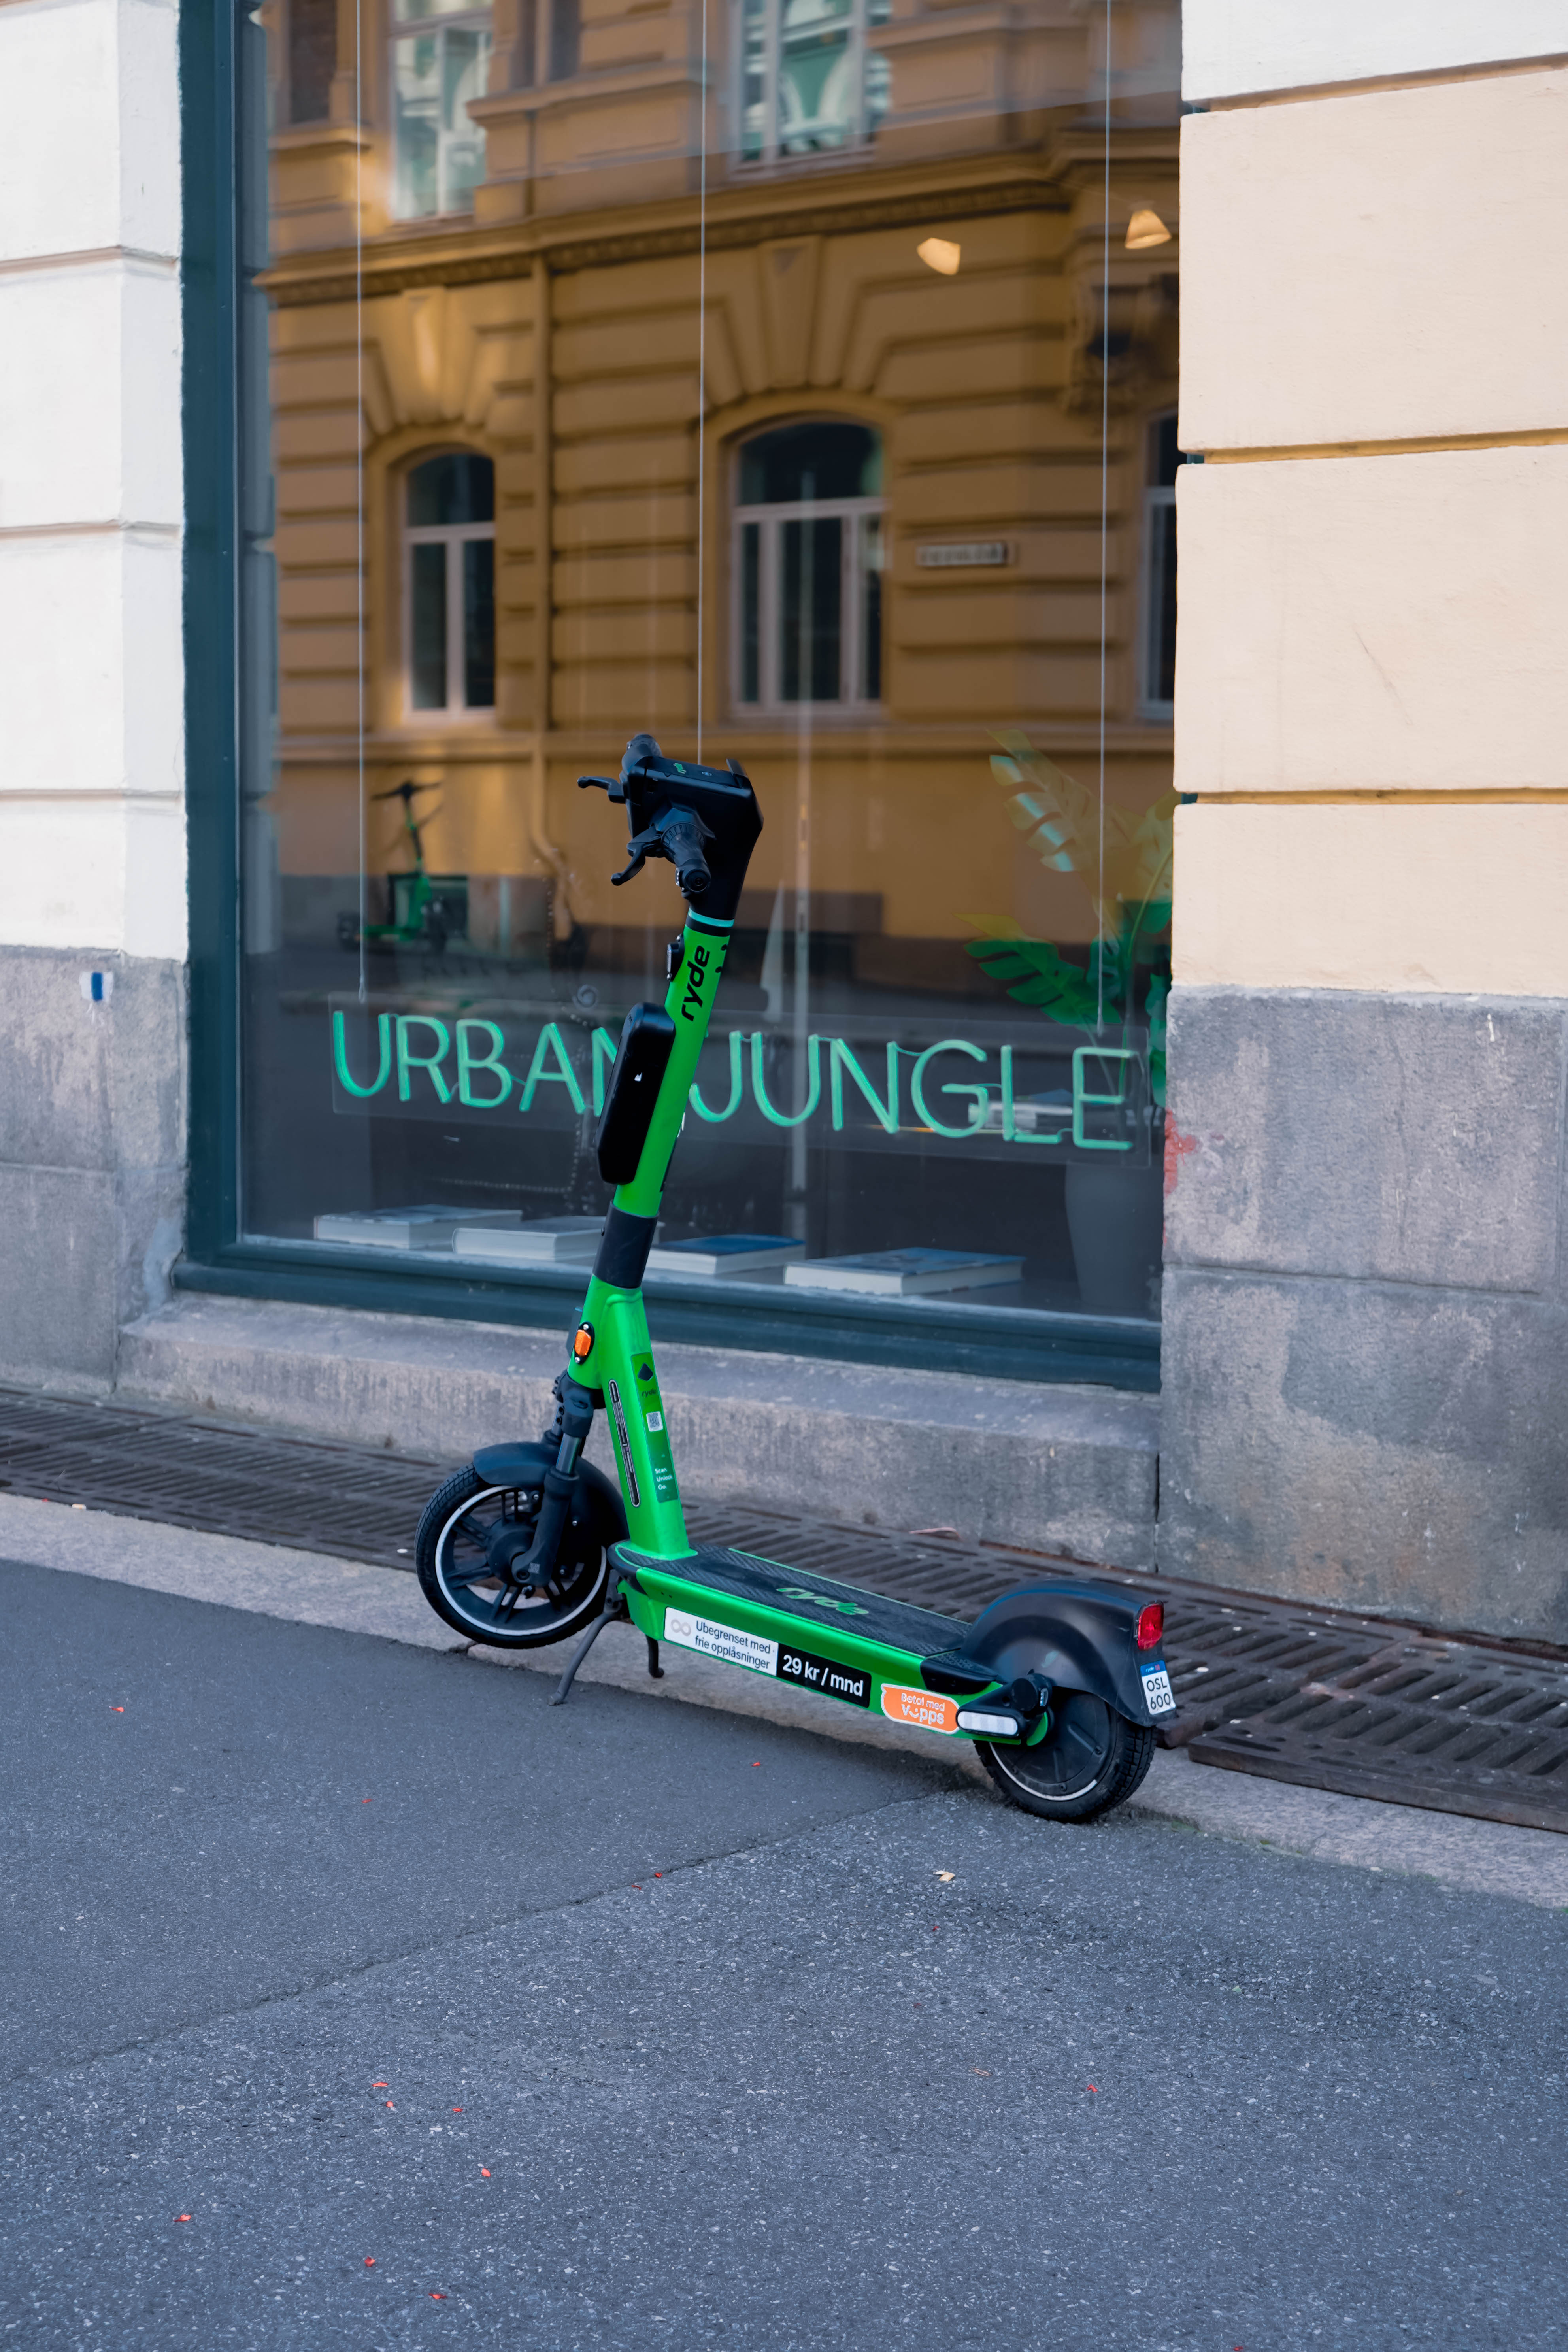
\includegraphics[width=\paperwidth,height=\paperheight]{src/Figures/Arriere_plan/Arriere_plan_Chap_4.jpg}
    }

% Rectangle
\AddToShipoutPictureBG*{
  \begin{tikzpicture}[remember picture,overlay]
    \node[fill=white, opacity=0.75, text width=\paperwidth, minimum height=11cm, anchor=north] 
    at ([yshift=-2cm]current page.north) {};
  \end{tikzpicture}
}

% Source
\AddToShipoutPictureFG*{
  \AtPageLowerRight{
    \raisebox{1cm}{
      \hspace{16cm}
      
\begin{tikzpicture}
        \node[fill=white, rounded corners=5pt, inner sep=5pt, align=center] {
          \tiny{Photography: \textcolor{blue}{Dylan Moinse (2023)}}
        };
      \end{tikzpicture}
    }
  }
}

    % ___________________________________________
    % Mini Table of Contents
    \cleardoublepage
    \setcounter{tocdepth}{2}
    % Redefine local table of contents title
    \renewcommand{\localcontentsname}{Table of Contents for Chapter~4}
\localtableofcontents

% Réinitialiser numérotation section
\setcounter{section}{0}

    % ___________________________________________
    % Graphical abstract
    \newpage
\section*{Key Points of Chapter~4
    \label{chap4:graphical-abstract}
    }
    \markright{Chapter Preambule}{}

\begin{figure}[h!]\vspace*{4pt}
        \caption*{}
        \label{graphical-abstract-chap4}
        \centerline{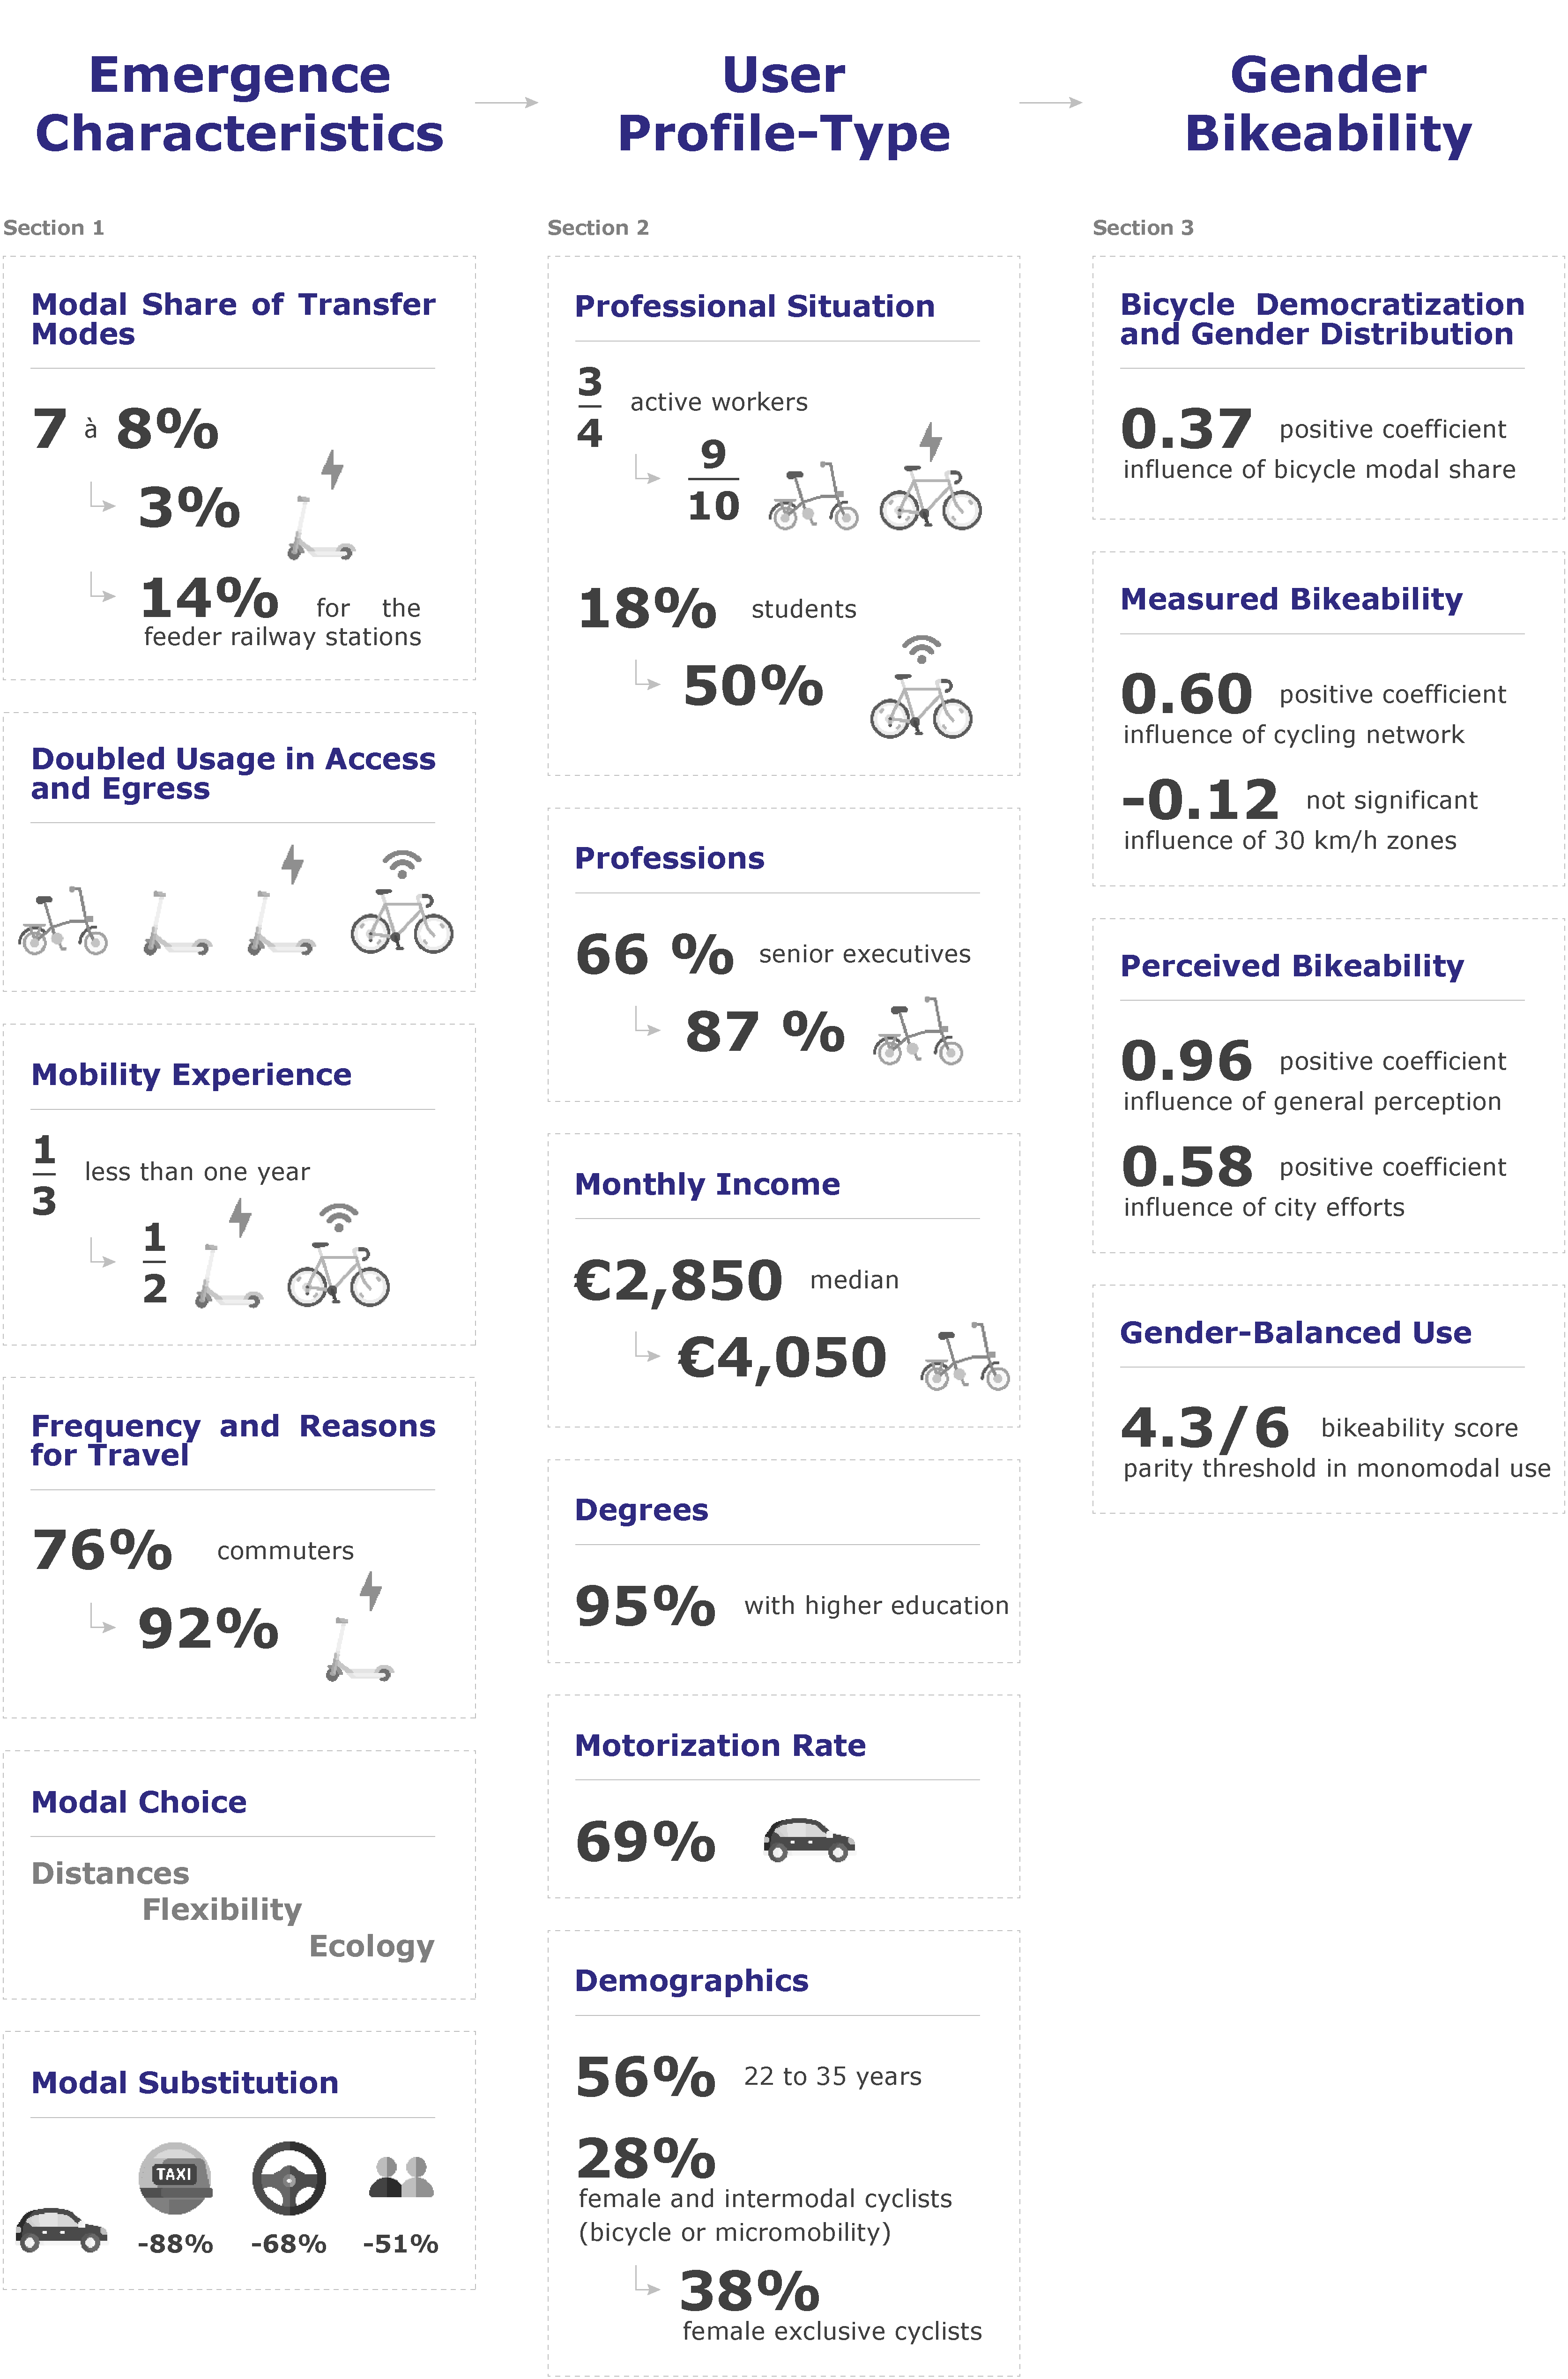
\includegraphics[width=1\columnwidth]{src/Figures/Graphical-abstract/EN_Graphical_abstract_chap4.pdf}}
        \vspace{5pt}
    \end{figure}

    % ___________________________________________
    % Preamble
    \newpage
    \begin{tcolorbox}[colback=white!5!white,
                      colframe=blue!75!blue,
                      title=
                      \bigskip
                      \center{\textbf{Preamble of Chapter~4}}
                      \\
                      \raggedright{\small{Chapter composed of \pagedifference{chap4:titre}{chap5:titre} pages, including \pagedifference{chap4:bibliographie}{chap5:titre} pages of bibliography}}
                      \bigskip]
\Large{\textcolor{blue}{\textbf{Abstract:}}}
    \\
\small{
This chapter explores the emergence and diversification of the integration of light individual mobility into public transport systems. The focus is on their modal synergy by examining the intermodal practices of users.%%Translated%%
    \\
The \hyperref[section-chap4:progression-velo-micromobilite-aubaine]{first section} (page~\pageref{section-chap4:progression-velo-micromobilite-aubaine}) aims to quantify the modal share of bicycles and micromobility in association with the rail system, analyzing adoption rates according to geographical contexts and transfer segments, before or after the main journey. The results show not only an underestimated modal share of these transfer modes with the rail system, estimated at 8\%, but also a trend towards growth in this usage. Contrary to popular belief, this modal share is higher in suburban areas than in urban centers. The adoption of these intermodal practices is recent for a significant proportion of users and tends to replace the use of transfer buses and cars, without substituting walking.%%Translated%%
    \\
However, these mobility practices remain unequal, attracting primarily adult men, highly skilled and with relatively high incomes. The \hyperref[section-chap4:profil-sociodemographique]{second section} (page~\pageref{section-chap4:profil-sociodemographique}) thus addresses the issue of the inclusivity of intermodal practices, providing a socio-demographic profile of intermodal cyclists and identifying the potential for modal shift to these mobility solutions.%%Translated%%
    \\
Finally, the \hyperref[section-chap4:cyclabilite-genre]{third section} (page~\pageref{section-chap4:cyclabilite-genre}) presents a case study on gender disparities in the monomodal and intermodal use of these vehicles, highlighting the importance of territorial design, the urban environment, and their perception in fostering more equitable access to these modes of transport. The statistical modeling identifies a positive association between perceived bikeability, objective bikeability, the modal share of bicycles, and the proportion of female cyclists, suggesting that improving the \textsl{bicycle system} and the \textsl{general perception} of \textsl{bike climate} is crucial to promoting a more inclusive use of bicycles and micromobility.%%Translated%%
    }
    \tcblower
\Large{\textcolor{blue}{\textbf{Keywords:}}}
    \\
    \small{
Modal choice;
Mobility behaviors;
Modal competitiveness;
Perceived bikeability;
Commuting trips;
Gender;
Socio-economic inequalities;
Inclusive mobility;
Modal share;
Emerging practices
    }
    \end{tcolorbox}

    % ___________________________________________
    % 4.*.
    \newpage
    \needspace{1\baselineskip} % Reserve space
    \addcontentsline{toc}{section}{Introduction of Chapter~4}
    \sectionheader{Introduction of Chapter~4}
\section*{Introduction of Chapter~4
    \label{chap4:introduction}
    }
    \markright{Introduction of Chapter~4}{} 

    % Citation
    \begin{displayquote}
\Commas{\textsl{The accessibility paradigm in transportation and land-use planning has become closely associated with both multimodalism and an equity-based view of transportation.} [\dots] \textsl{Accessibility is a resource that is the desired benefit provided by transportation; that resource can be distributed equitably or inequitably. All populations benefit when their accessibility increases, though some populations start from a position of greater accessibility deficit. Under the accessibility shift, transportation analysis focuses on system performance with respect to population rather than with respect to pieces of infrastructure.}}

\textcolor{blue}{Jonathan} \textcolor{blue}{\textcite[16-17]{levine_mobility_2019}}\index{Levine, Jonathan|pagebf}\index{Grengs, Joe|pagebf}\index{Merlin, Louis~A.|pagebf}. \foreignlanguage{english}{\textsl{From Mobility to Accessibility: Transforming Urban Transportation and Land-Use Planning}}, Cornell University Press, Ithaca, 240~p. ISBN: \href{https://search.worldcat.org/fr/title/1393973234}{978-1-5017-1608-9}
    \end{displayquote}

% Introduction
\lettrine[lines=3, findent=8pt, nindent=0pt]{\lettrinefont T}{his} first chapter dedicated to the empirical results of this doctoral research undertakes an investigation into \textsl{intermodal practices} as study objects, characterized by the integration of light individual mobility into public transport networks. This section examines the individual dimension of \gls{accessibility}, exploring the current developments of mobility systems as well as the behaviors and profiles of users adopting these modal combinations. The aim of this study is to demonstrate the relevance of this research topic within the French context, specifically in the Hauts-de-France region, highlighting the rise of these modes of transport and their interactions \textcolor{blue}{\autocites[77]{oostendorp_combining_2018}[56]{ensor_mode_2021}}\index{Oostendorp, Rebekka|pagebf}\index{Gebhardt, Laura|pagebf}\index{Ensor, Matt|pagebf}\index{Maxwell,~O.|pagebf}\index{Bruce, Oliver|pagebf} amidst ongoing \Commas{modal hybridization} \textcolor{blue}{\autocite[15]{amar_homo_2016}}\index{Amar, Georges|pagebf}.%%Translated%%

% Research Objectives
Given the general lack of knowledge about \gls{micromobility}, which is currently in the process of \Commas{emergence}, particularly regarding the ownership of personal vehicles \textcolor{blue}{\autocites{richer_dossier_2021}[19]{pages_nouveaux_2021}}\index{Pages, Thibaud|pagebf}\index{Lammoglia, Adrien|pagebf}\index{Josselin, Didier|pagebf}\index{Richer, Cyprien|pagebf} and their connections with public transport (see the gaps in the literature identified in \hyperref[chap2:titre]{Chapter~2}, page~\pageref{chap2:titre}), this chapter aims to clarify the role and contribution of these vehicles in relation to the definition of an \acrfull{M-TOD}, while providing an overview of users. This research work is thus based on train stations, locations where modal practices integrating \gls{bicycle} and micromobility are observed, with the aim of highlighting this mobility phenomenon, which is becoming increasingly visible in these strategic exchange locations. The central question of this empirical research is to explore and characterize the intermodal practices that include light individual mobility in various territorial contexts and at a regional or even national scale. Three objectives structure the present chapter:
\begin{customitemize}
    \item \textsl{Determine the modal share of light individual mobility integrated into the rail system, based on geographical contexts}. This analysis quantifies intermodal adoption from estimates of the modal share of bicycles and micromobility as transfer modes, addressing their emergence in various territorial configurations while distinguishing access and egress segments. The originality of this approach lies in its ability to compare various vehicles, a relatively rare approach in the literature;
    \item \textsl{Study the inclusive dimension of intermodal practices}. This section provides a portrait of intermodal travelers, based on a grid of capitals, to identify the potential for modal shift towards these mobility solutions;
    \item \textsl{Case study on the gender distribution of exclusive and intermodal use of bicycles and micromobility, linked to territorial design}. This investigation focuses on the inclusive dimension of accessibility connected to the quality of public space design, defining a statistical model that captures levers to reduce inequalities in access to these modes of transport. The approach of \Commas{territorial hospitality}, which has evolved and diversified over time, serves as a conceptual reference to assess territorial design as well as public policies in terms of welcoming cyclists and retaining users by meeting their needs \textcolor{blue}{\autocite[3]{talandier_lhospitalite_2023}}\index{Talandier, Magali|pagebf}.
\end{customitemize}%%Translated%%

% Plan Introduction 1
We will begin by quantifying and characterizing emerging intermodal practices to understand how they represent an opportunity for public transport services (\hyperref[section-chap4:progression-velo-micromobilite-aubaine]{Section~1}, page~\pageref{section-chap4:progression-velo-micromobilite-aubaine}). The first section will assess the modal share of each light individual mobility vehicle when integrated into the rail network, while contextualizing these measures based on the urban or \gls{peri-urban} nature of the territory and whether the journey by bicycle or micromobility falls within a \Commas{first} or \Commas{last mile} logic (\hyperref[chap4:proportion-croissante-voyageurs-intermodaux]{sub-section~1.1}, page~\pageref{chap4:proportion-croissante-voyageurs-intermodaux}). The second sub-section will explore the mobility behaviors of intermodal cyclists to better understand the impact of modal adoption on existing mobility systems, identifying motivations and substitution effects that arise from it (\hyperref[chap4:comportements-mobilite]{sub-section~1.2}, page~\pageref{chap4:comportements-mobilite}).

% Plan Introduction 2
The second section will provide a portrait of intermodal cyclists, comparing them to rail travelers in general and to the French population, in order to identify the specificities of this social group of mobile individuals (\hyperref[section-chap4:profil-sociodemographique]{Section~2}, page~\pageref{section-chap4:profil-sociodemographique}). We will begin by examining the economic resources, professional status, and level of qualification of these users, considering the economic and cultural capitals at their disposal (\hyperref[chap4:capital-economique-culturel]{sub-section~2.1}, page~\pageref{chap4:capital-economique-culturel}). Next, we will describe the material capitals and daily mobility practices, aiming to create a snapshot of these individuals (\hyperref[chap4:capital-mobilite]{sub-section~2.2}, page~\pageref{chap4:capital-mobilite}). Finally, we will address the demographic attributes of intermodal cyclists, considering criteria related to age and \gls{gender}, with an emphasis on inclusive mobility (\hyperref[chap4:demographie]{sub-section~2.3}, page~\pageref{chap4:demographie}). This analysis will set the stage for the final section of this chapter.

% Plan Introduction 3
The third part will explore the interactions between the gendered use of these mobility solutions and the moderating role of urban planning, through the lens of territorial hospitality. This section will investigate the relational dynamics between gender-related issues and urban design (\hyperref[section-chap4:cyclabilite-genre]{Section~3}, page~\pageref{section-chap4:cyclabilite-genre}). We will begin by describing the analytical framework, developed through the use of databases alongside our empirical material (\hyperref[chap4:materiau-empirique-genre]{Section~3.1}, page~\pageref{chap4:materiau-empirique-genre}), which will take the form of a statistical model (\hyperref[chap4:methodologie-modele-ols]{Section~3.2}, page~\pageref{chap4:methodologie-modele-ols}). Based on the explained approach, we will present the links between cycling accessibility, both objective and perceived, and the gendered practice of light individual mobility (\hyperref[section-chap4:cyclabilite-territoires-genre]{Section~3.3}, page~\pageref{section-chap4:cyclabilite-territoires-genre}).

% Plan Introduction 4
In conclusion, we will summarize the main contributions of this study, aiming to provide a general overview of cyclists and their mobility practices in an intermodal context, as well as to refocus the issues of social inclusivity from the perspective of territorial planning (\hyperref[chap4:conclusion]{Chapter~4 conclusion}, page~\pageref{chap4:conclusion}).

% ___________________________________________
% 4.1.
\newpage
\needspace{1\baselineskip} % Réserve de l'espace
\sectionheader{Growing Adoption of Light Individual Mobility}
\section{The Joint Progress of Bicycles and Micromobility: A Boon for Public Transport Networks
    \label{section-chap4:progression-velo-micromobilite-aubaine}
    }

% Introduction
Intermodal practices, which involve the modal synergy of public transport, bicycles, and micromobility, are expected to develop rapidly \textcolor{blue}{\autocite[4]{kostrzewska_towards_2017}}\index{Kostrzewska, Małgorzata|pagebf}\index{Macikowski, Bartosz|pagebf}, as they meet mobility needs related to the \Commas{first and last miles} \textcolor{blue}{\autocite[29]{holm_moller_micromobility_2020}}\index{Holm Møller, Thomas|pagebf}\index{Simlett, John|pagebf}\index{Mugnier, Eric|pagebf}. Based on this projection, our research aims to confirm the first hypothesis, which suggests that bicycles are experiencing a revival and simultaneous expansion alongside micromobility, and to test the second hypothesis, which posits that the renewed focus on proximity presents an opportunity for public transport systems. By utilizing data from quantitative observation and a survey distributed to users at train stations, we aim to provide a comprehensive picture of these mobility behaviors and examine their implications. This approach not only seeks to offer a detailed overview of intermodal practices but also aims to lay the groundwork for further discussions on their integration into the principles of \acrfull{TOD}.%%Translated%%

% Annonce du plan
This first section, dedicated to the evolution of the integration of light individual mobility, seen as a boon for public transport networks, is divided into two distinct phases. First, we will examine the relevance of the term \textsl{emergence} to describe the observed intermodal practices (see the \hyperref[chap4:proportion-croissante-voyageurs-intermodaux]{section on the growing proportion of intermodal travelers}, page~\pageref{chap4:proportion-croissante-voyageurs-intermodaux}). This exploration will include an assessment of the modal shares attributed to these transfer modes, cross-referenced with users' intermodal experiences, the \gls{cartography} of origin and destination flows, as well as the specifics of each segment of intermodal trips. Subsequently, our focus will shift to the mobility behaviors of intermodal cyclists (see the \hyperref[chap4:comportements-mobilite]{section on the characteristics of commuters}, page~\pageref{chap4:comportements-mobilite}), in order to better understand the contours of these intermodal practices and assess their impact on the coexistence of mobility systems. This will involve an analysis of usage frequency, related to the motivations for making a \gls{journey}, the reasons behind the adoption of these modes, the modal substitution effect, and the resulting changes in mobility.%%Translated%%

% 4.1.1.
\needspace{1\baselineskip} % Réserve de l'espace
\subsection{A Growing Proportion of Intermodal Cyclists, Driven by the Rise of Personal and Shared Micromobility
    \label{chap4:proportion-croissante-voyageurs-intermodaux}
    }

% Introduction
In this subsection, we explore the intermodal dimension of light individual mobility within the regional rail network, with a particular focus on how emerging transport modes, such as \acrfull{PeS}, contribute to enhancing the attractiveness and improving the accessibility of public transport systems \textcolor{blue}{\autocite[45]{corporate_partnership_board_good_2020}}\index{Corporate Partnership Board@\textsl{Corporate Partnership Board}|pagebf}, both in urban centers and in peri-urban areas \textcolor{blue}{\autocite[38]{stransky_periurbain_2019}}\index{Stransky, Vaclav|pagebf}. This analysis focuses on the train stations of the Hauts-de-France region, where we aim to quantify the modal share of bicycles and micromobility, in connection with transport hubs, in order to highlight their growing importance as objects of study. Our goal is also to place the estimated modal shares of these transfer modes in various urban contexts.%%Translated%%

% 4.1.1.1.
\needspace{1\baselineskip} % Réserve de l'espace
\subsubsection*{Modal Share of Light Individual Mobility in Association with the Rail Network
    \label{chap4:part-modale-velo-micromobilite}
    }

% Introduction
During this doctoral research, an investigation of nine train stations in the Hauts-de-France region first allowed for the implementation of quantitative observation, as outlined in the \hyperref[chap3:observation-quantitative-gares-examinees]{methodological section dedicated to the examined stations} (page~\pageref{chap3:observation-quantitative-gares-examinees}) in \hyperref[chap3:titre]{Chapter~3} (page~\pageref{chap3:titre}). This statistical analysis resulted in the creation of a descriptive sample consisting of 15,435 rail travelers. Among these users, 1,035 individuals, representing 6.71\% of the total sample, were identified as accompanied by a bicycle or a micromobility option on the platforms.%%Translated%%

% Part modale globale de l'embarquement (observation)
This observation suggests that, during peak periods typically associated with work and school commutes, as well as in the selected stations considered representative of the diversity of urban contexts in the region, fewer than 7\% of passengers on the \acrfull{HST}, \acrfull{TERGV}, and \acrfull{TER} carry a mode of transport falling under light individual mobility\footnote{~
    Note that this proportion excludes intermodal cyclists who parked their vehicle before boarding the train or who retrieve it upon alighting, as well as shared mobility services.
}.%%Translated%%

% Part modale détails de l'embarquement (observation)
As part of this study on the boarding modalities of light transport modes on trains, the observation sessions indicate a predominance of all types of scooters, representing 3.65\% (564 observations) of the total. This is closely followed by bicycles, across all categories, which account for 2.93\% (452 observations) of the cases observed. Other forms of \acrfull{PMD} devices constitute 0.12\% (19 observations). More specifically, the distribution of light individual mobility types on board is as follows (see \hyperref[fig-chap4:part-modale-detaillee-mobilite-individuelle-legere]{Figure \ref{fig-chap4:part-modale-detaillee-mobilite-individuelle-legere}}, page~\pageref{fig-chap4:part-modale-detaillee-mobilite-individuelle-legere}). The \acrshort{PeS} leads with 2.98\% (460 observations), demonstrating its rapid and widespread adoption, even surpassing conventional bicycles in the rail context. The latter holds a modal share of 2.13\% (329 observations) in transfer. Folding bicycles and mechanical scooters account for 0.80\% and 0.67\% (122 and 104 observations), respectively, while skateboards and unicycles are much less represented, with 0.07\% and 0.05\% (11 and 8 observations), respectively. These statistical results highlight that the \acrshort{PeS} proves to be a mode of transport particularly suited for train boarding, due to its lightness and compactness.%%Translated%%

% Figure part modale détaillée
\begin{figure}[h!]\vspace*{4pt}
    \caption{Estimation of the Modal Share of Light Individual Mobility Onboard and Integrated into the Train, in the Hauts-de-France Region.}
    \label{fig-chap4:part-modale-detaillee-mobilite-individuelle-legere}
    \centerline{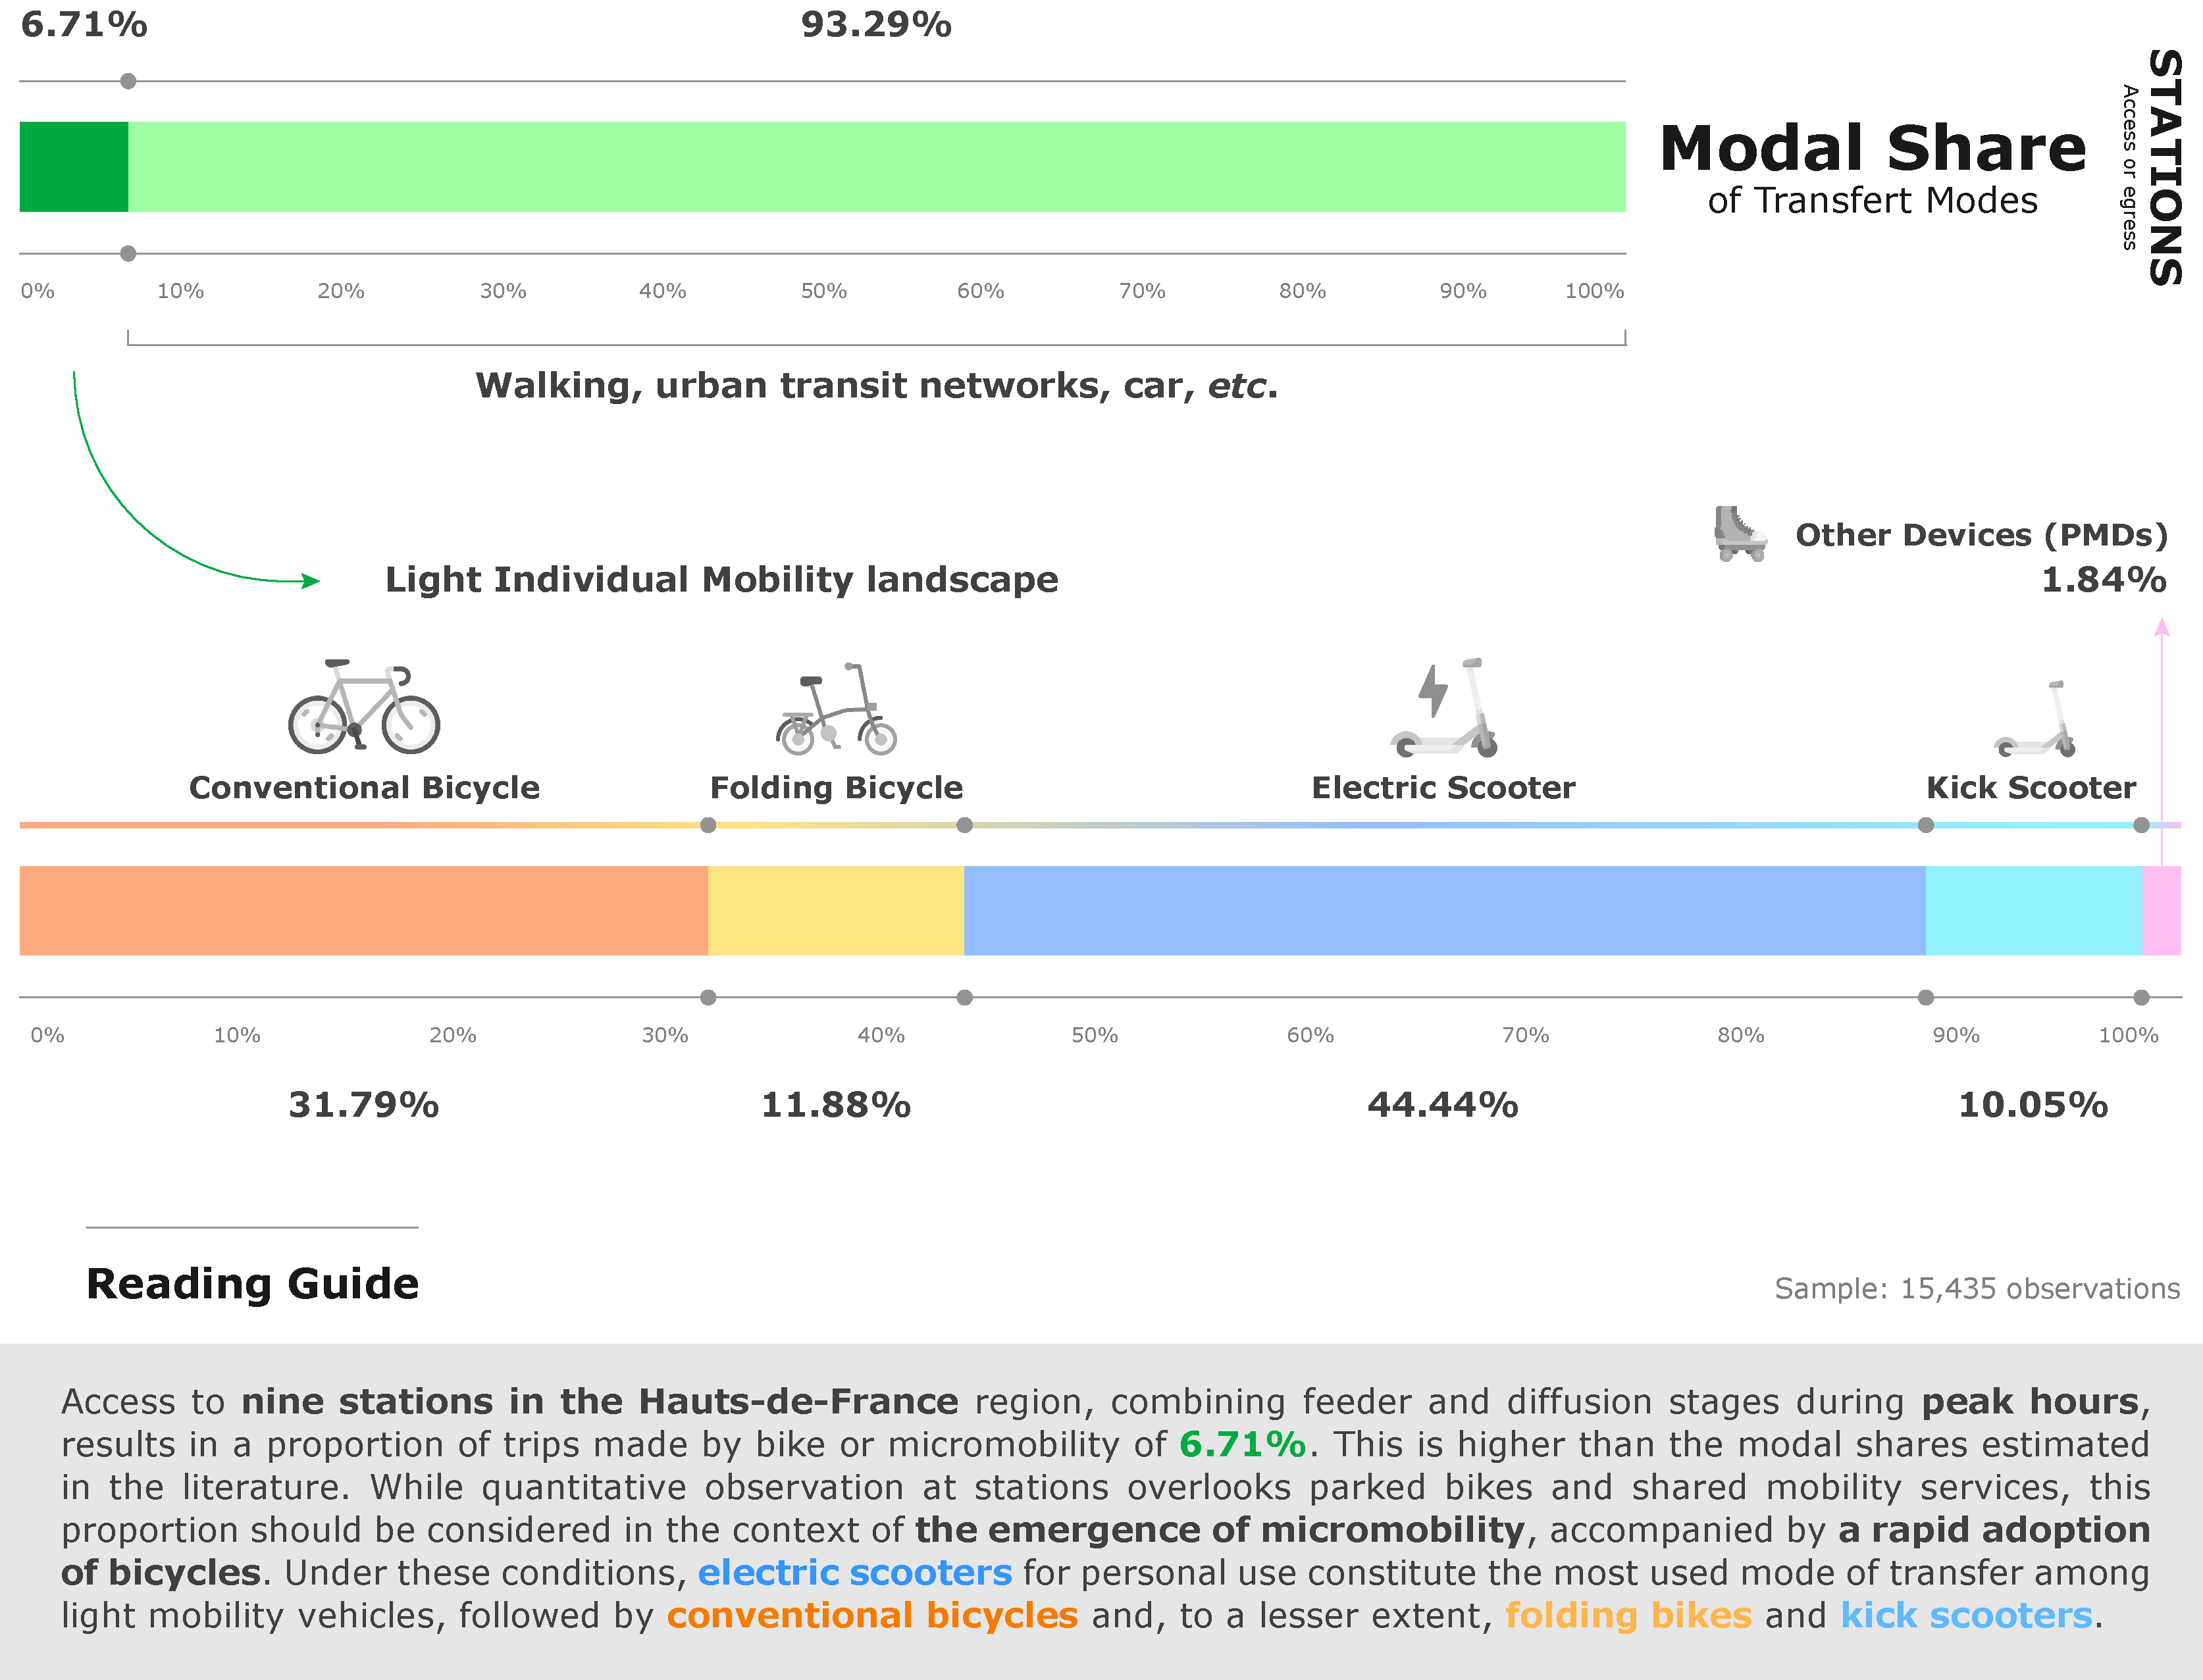
\includegraphics[width=1\columnwidth]{src/Figures/Chap-4/EN_Observation_quantitative_part_modale.pdf}}
    \vspace{5pt}
    \begin{flushright}\scriptsize{
    Author: \textcolor{blue}{Dylan Moinse (2022)}
    }\end{flushright}
\end{figure}

% Part modale globale intermodale (questionnaire)
The quantification of intermodal use of light individual mobility was enriched by data collected through the survey addressed to users\footnote{~
    It should be noted, however, that the contribution of the survey should be viewed in the context of direct observation, taking into account the smaller sample size and the national scale, which includes a broader diversity of public transport systems, even though the \acrshort{HST} and \acrshort{TER} remain predominant.
}. As shown in \hyperref[table-chap4:part-modale-vehicules-intermodalite]{Table~\ref{table-chap4:part-modale-vehicules-intermodalite}} (page~\pageref{table-chap4:part-modale-vehicules-intermodalite}), of 100 rail travelers involved in an intermodal trip integrating light individual mobility, 68 of them reported using a bicycle (147 responses), while 22 opted for a scooter (48 responses), 7 for a bike or micromobility service (16 responses), and 3 for another form of \acrshort{PMD} (6 responses). Among these intermodal travelers, 78\% brought their vehicle on the rail network (169 responses). 50\% of users opted for a conventional bicycle (110 responses), with a quarter of these cyclists choosing to park their bike. Regarding the use of the \acrshort{PeS}, it was adopted by 18\% of respondents (39 responses). 11\% of them traveled with a mechanical folding bicycle (24 responses). It is noteworthy that all respondents who used these two folding vehicles consistently brought them onboard mass transit services.%%Translated%%

    % Tableau Part modale intermodale - modes de transfert
% Table Modal Share of Intermodal Light Mobility - Transfer Modes
%%Rédigé%%
    \begin{table}[h!]
    \centering
    \renewcommand{\arraystretch}{1.5}
    \resizebox{\columnwidth}{!}{
    \begin{tabular}{p{0.50\columnwidth}p{0.15\columnwidth}p{0.17\columnwidth}p{0.18\columnwidth}}
        %\hline
    \rule{0pt}{15pt} \small{\textbf{\textcolor{blue}{Type of Vehicle}}} & \small{\textbf{\textcolor{blue}{Observation}}} & \small{\textbf{\textcolor{blue}{Survey}}} & \small{\textbf{\textcolor{blue}{Boarding}}}\\
        \hline
\small{\textbf{All types of light individual mobility combined}} & \multirow{1.5}{*}{\small{\textbf{100.00\%}}} & \multirow{1.5}{*}{\small{\textbf{100.00\%}}} & \multirow{1.5}{*}{\small{\textbf{77.88\%}}}\\
        \hdashline
\small{\textbf{All types of personal bicycles}} & \small{\textbf{43.67\%}} & \small{\textbf{67.74\%}} & \small{\textbf{78.91\%}}\\
\small{Conventional bicycle} & \small{31.79\%} & \small{49.77\%} & \small{75.93\%}\\
\small{Folding bicycle} & \small{11.88\%} & \small{11.06\%} & \small{100.00\%}\\
\small{Electric bicycle (\acrshort{e-Bike})} & \small{-} & \small{3.69\%} & \small{50.00\%}\\
\small{Electric folding bicycle} & \small{-} & \small{2.76\%} & \small{100.00\%}\\
\small{Cargo bicycle} & \small{-} & \small{0.46\%} & \small{0.00\%}\\
        \hdashline
\small{\textbf{All types of personal scooters}} & \small{\textbf{54.49\%}} & \small{\textbf{22.12\%}} & \small{\textbf{100.00\%}}\\
\small{Personal electric scooter (\acrshort{PeS})} & \small{44.44\%} & \small{17.97\%} & \small{100.00\%}\\
\small{Mechanical scooter} & \small{10.05\%} & \small{4.15\%} & \small{100.00\%}\\
        \hdashline
\small{\textbf{Other types of \acrfull{PMD}}} & \multirow{1.5}{*}{\small{\textbf{1.84\%}}} & \multirow{1.5}{*}{\small{\textbf{2.76\%}}} & \multirow{1.5}{*}{\small{\textbf{83.33\%}}}\\
\small{\textsl{Skateboard}} & \small{1.06\%} & \small{1.38\%} & \small{100.00\%}\\
\small{Monowheel} & \small{0.77\%} & \small{0.92\%} & \small{100.00\%}\\
\small{Gyropod} & \small{-} & \small{0.46\%} & \small{0.00\%}\\
        \hdashline
\small{\textbf{All types of shared vehicles}} & \small{\textbf{-}} & \small{\textbf{7.37\%}} & \small{\textbf{0.00\%}}\\
\small{Public bike-sharing (\acrshort{PBS})} & \small{-} & \small{6.45\%} & \small{0.00\%}\\
\small{Electric bike in free-floating (\acrshort{DBS})} & \small{-} & \small{0.46\%} & \small{0.00\%}\\
\small{Electric scooter in free-floating (\acrshort{DESS})} & \multirow{1.5}{*}{\small{-}} & \multirow{1.5}{*}{\small{0.46\%}} & \multirow{1.5}{*}{\small{0.00\%}}\\
        \hline
        \end{tabular}}
    \caption{Share of each transfer vehicle type within light individual mobility in France.}
    \label{table-chap4:part-modale-vehicules-intermodalite}
        \vspace{5pt}
        \begin{flushleft}\scriptsize{
        \textcolor{blue}{Note:} The \textsl{Observation} column refers to the subsample obtained from the quantitative observation of travelers (1,035 counts), while the \textsl{Survey} column refers to the intermodal trips declared by participants (217 responses), and the \textsl{Boarding} modality quantifies the share of vehicles carried onboard public transport.
        \\
        \textcolor{blue}{Reading Guide:} The modal share of cycles used for intermodal transfers shows that electric scooters and bicycles, particularly folding ones, for personal use have the largest shares. The electric vehicle and both conventional and electric folding bicycles, as well as light mobility devices such as skateboards and monowheels, all have a 100\% boarding rate.
        }\end{flushleft}
        \begin{flushright}\scriptsize
        Author: \textcolor{blue}{Dylan Moinse (2022)}
        \end{flushright}
        \end{table}%%Rédigé%%

% Confrontation questionnaire
The data extracted from the survey provide additional insights into the discrepancies observed in the combined use of light individual mobility with public transport. The analysis highlights the notable difference in modal shares for bicycles, compared to the results of the quantitative observation, which may be explained by the non-inclusion of parked bicycles during the observation sessions. Furthermore, the significant discrepancy regarding the \acrshort{PeS} suggests that the survey responses might not accurately reflect the intermodal practices as observed at the train stations. This distortion could stem from an overrepresentation of cyclists among the respondents, implying that members of this community were particularly inclined to participate in the survey. It is clear that the bicycle, in its various forms and with its different parking or boarding modalities, plays a dominant role in the intermodal use of light individual mobility. In this respect, the \Commas{little queen} contributes between 45\% and 70\% of these intermodal practices. On the other hand, the \acrshort{PeS} accounts for between 20\% and 45\% of the observed and reported behaviors.%%Translated%%

% Part modale déterminée
By integrating information from the survey and extrapolating the observed modal shares, we are able to establish a global estimate of the modal share of light individual mobility as transfer modes to and from the train stations in the Hauts-de-France region. According to the survey responses, approximately a quarter of commuters opt for parking their light vehicle, particularly among cyclists. As a result, the modal share of bicycles in \gls{intermodality} would be re-estimated at 2.64\% (408 users) among the total flow of travelers. In addition, we included a subgroup of users of \acrfull{PBS}, \acrfull{DBS}, and \acrfull{DESS} systems, accounting for 7.37\% (89 users). This brings the total to 1,202 intermodal cyclists, allowing us to conclude that the estimated modal share reaches 7.79\%. This analysis thus provides a more complete and adjusted view of the use of light individual mobility in the intermodal context.%%Translated%%

% Littérature part modale vélo
The scientific and technical literature related to the determination of train station usage by cyclists in feeder services is abundant and corroborates the results obtained, which allowed us to estimate the modal share for conventional bicycles at 2.64\% in the stations studied in France. Regarding the Hauts-de-France stations, a recent study by \textcolor{blue}{\textcite[20]{hasiak_estimation_2023}}\index{Hasiak, Fabrice|pagebf}\index{Verdier, Laurent|pagebf} reports a modal share for conventional bicycles of 2\% in \gls{access} and 1\% in \gls{egress}, based on the aggregation of various survey data. In the specific case study of the Amboise station (Centre-Val de Loire), 7\% of travelers access the station by bike, with half bringing their vehicles on board and the other half parking them \textcolor{blue}{\autocite[744]{midenet_modal_2018}}\index{Midenet, Sophie|pagebf}\index{Côme, Etienne|pagebf}\index{Papon, Francis|pagebf}. On a national level, the SNCF estimates that 6\% of \acrshort{TER} passengers travel by bike to reach a station \textcolor{blue}{\autocite[9]{coue_embarq_2021}}\index{Coué, Antoine|pagebf}. This proportion should be viewed in comparison with that observed in the Netherlands, where 30\% of access to regional hubs is by bike, compared to 25\% in Denmark, 16\% in Germany, and 3\% in the United Kingdom \textcolor{blue}{\autocite[285]{martens_bicycle_2004}}\index{Martens, Karel|pagebf}. Additionally, we were able to identify a boarding proportion for conventional bicycles reaching 76\%, indicating mobility behaviors that are much more pronounced than those reported by \textcolor{blue}{Christian} \textcolor{blue}{\textcite[5]{gioria_etude_2016}}\index{Gioria, Christian|pagebf}, who found that only 30\% to 50\% of intermodal bicycle trips involve boarding on certain \acrshort{TER} lines.%%Translated%%

% Littérature part modale mobilité individuelle légère
Regarding the integration of micromobility, the estimation of the distribution of transfer modes is also supported by secondary analysis of the survey we conducted in the Provence-Alpes-Côte d'Azur region, which highlights a modal share of 5\% for bicycles and 2\% for the \acrshort{PeS} \textcolor{blue}{\autocite[180]{moinse_intermodal_2022}}\index{Moinse, Dylan|pagebf}\index{Goudeau, Matthieu|pagebf}\index{L'Hostis, Alain|pagebf}\index{Leysens, Thomas|pagebf}. Correspondingly, 6\% of the flows to and from central train stations in France are made by bike or scooter, whether personal or self-service, according to the study conducted by the \textcolor{blue}{\textcite[18]{enov_enquete_2021}}\index{Enov@\textsl{Enov}|pagebf}. Furthermore, \textcolor{blue}{Christian} \textcolor{blue}{\textcite[5]{gioria_etude_2016}}\index{Gioria, Christian|pagebf} points out that, although station usage nationwide is around 2\% for light individual mobility, these figures vary significantly by region, with a 6\% share for stations directly connected to a heavy transport mode in urban areas.%%Translated%%

% Transition
The statistical results from this subsection highlight a relatively high modal share for light individual mobility, estimated at 8\%, which is higher than that typically reported in previous studies, around 2\% to 3\% in transfer. This finding can be explained by a better consideration of micromobility, particularly the \acrshort{PeS}, in the analysis of transfer modes. Shedding light on these often overlooked practices underscores the importance of integrating them into urban strategies such as \acrshort{TOD}. However, this recognition is not sufficient to confirm the novelty of these intermodal practices, as the mere identification of their prevalence does not necessarily demonstrate an \textsl{emergence}. In this regard, the following analysis is based on the responses to the survey distributed to intermodal users and aims to determine whether modal adoption is recent or, on the contrary, well established, depending on the different transport modes examined.%%Translated%%

% 4.1.1.2.
\needspace{1\baselineskip} % Réserve de l'espace
\subsubsection*{Emerging Nature of Intermodal Practices at Train Stations
    \label{chap4:emergence-pratiques-intermodales}
    }

% Introduction
In light of the discrepancies observed between the modal share of these transfer modes, determined by quantitative observation and survey responses, and the figures from the few studies addressing this topic, it is legitimate to question the identification of a trend in recent years. Can the mobility practices involving the integration of light individual mobility with public transport networks be considered \textsl{emerging}? To approach this reflection, we examined a specific question from the survey conducted, which asks participants about their intermodal experience: \Commas{How long have you been using this modal combination?} (see \hyperref[annexes:structure-questionnaire-usagers]{Annex~\ref{annexes:structure-questionnaire-usagers}}, page~\pageref{annexes:structure-questionnaire-usagers}). The aim is to determine whether the observed practices are a recent phenomenon, particularly driven by the diversification of light individual mobility and the development of electromobility.%%Translated%%

% Résultats globaux expérience intermodale
Starting from the observation of the growing prevalence of intermodal practices at train stations in recent years, mainly attributable to the rise of micromobility, particular attention was paid to the intermodal experience of these travelers (see \hyperref[fig-chap4:experience-intermodale]{Figure~\ref{fig-chap4:experience-intermodale}}, page~\pageref{fig-chap4:experience-intermodale}). The descriptive data drawn from the reported responses reveal that for 43\% of participants, encompassing all types of light individual mobility, these modal combinations with rail networks have been adopted for \Commas{several years} (94 responses). Furthermore, 21\% and 16\% of respondents reported having an intermodal experience dating back to approximately \Commas{one year} and \Commas{a few months}, respectively (45 and 35 responses). Additionally, 13\% of respondents tried this modal combination for the first time during the administration of the survey (29 responses).%%Translated%%

% Figure expérience intermodale
\begin{figure}[h!]\vspace*{4pt}
    \caption{Declared Intermodal Experience of Intermodal Cyclists.}
    \label{fig-chap4:experience-intermodale}
    \centerline{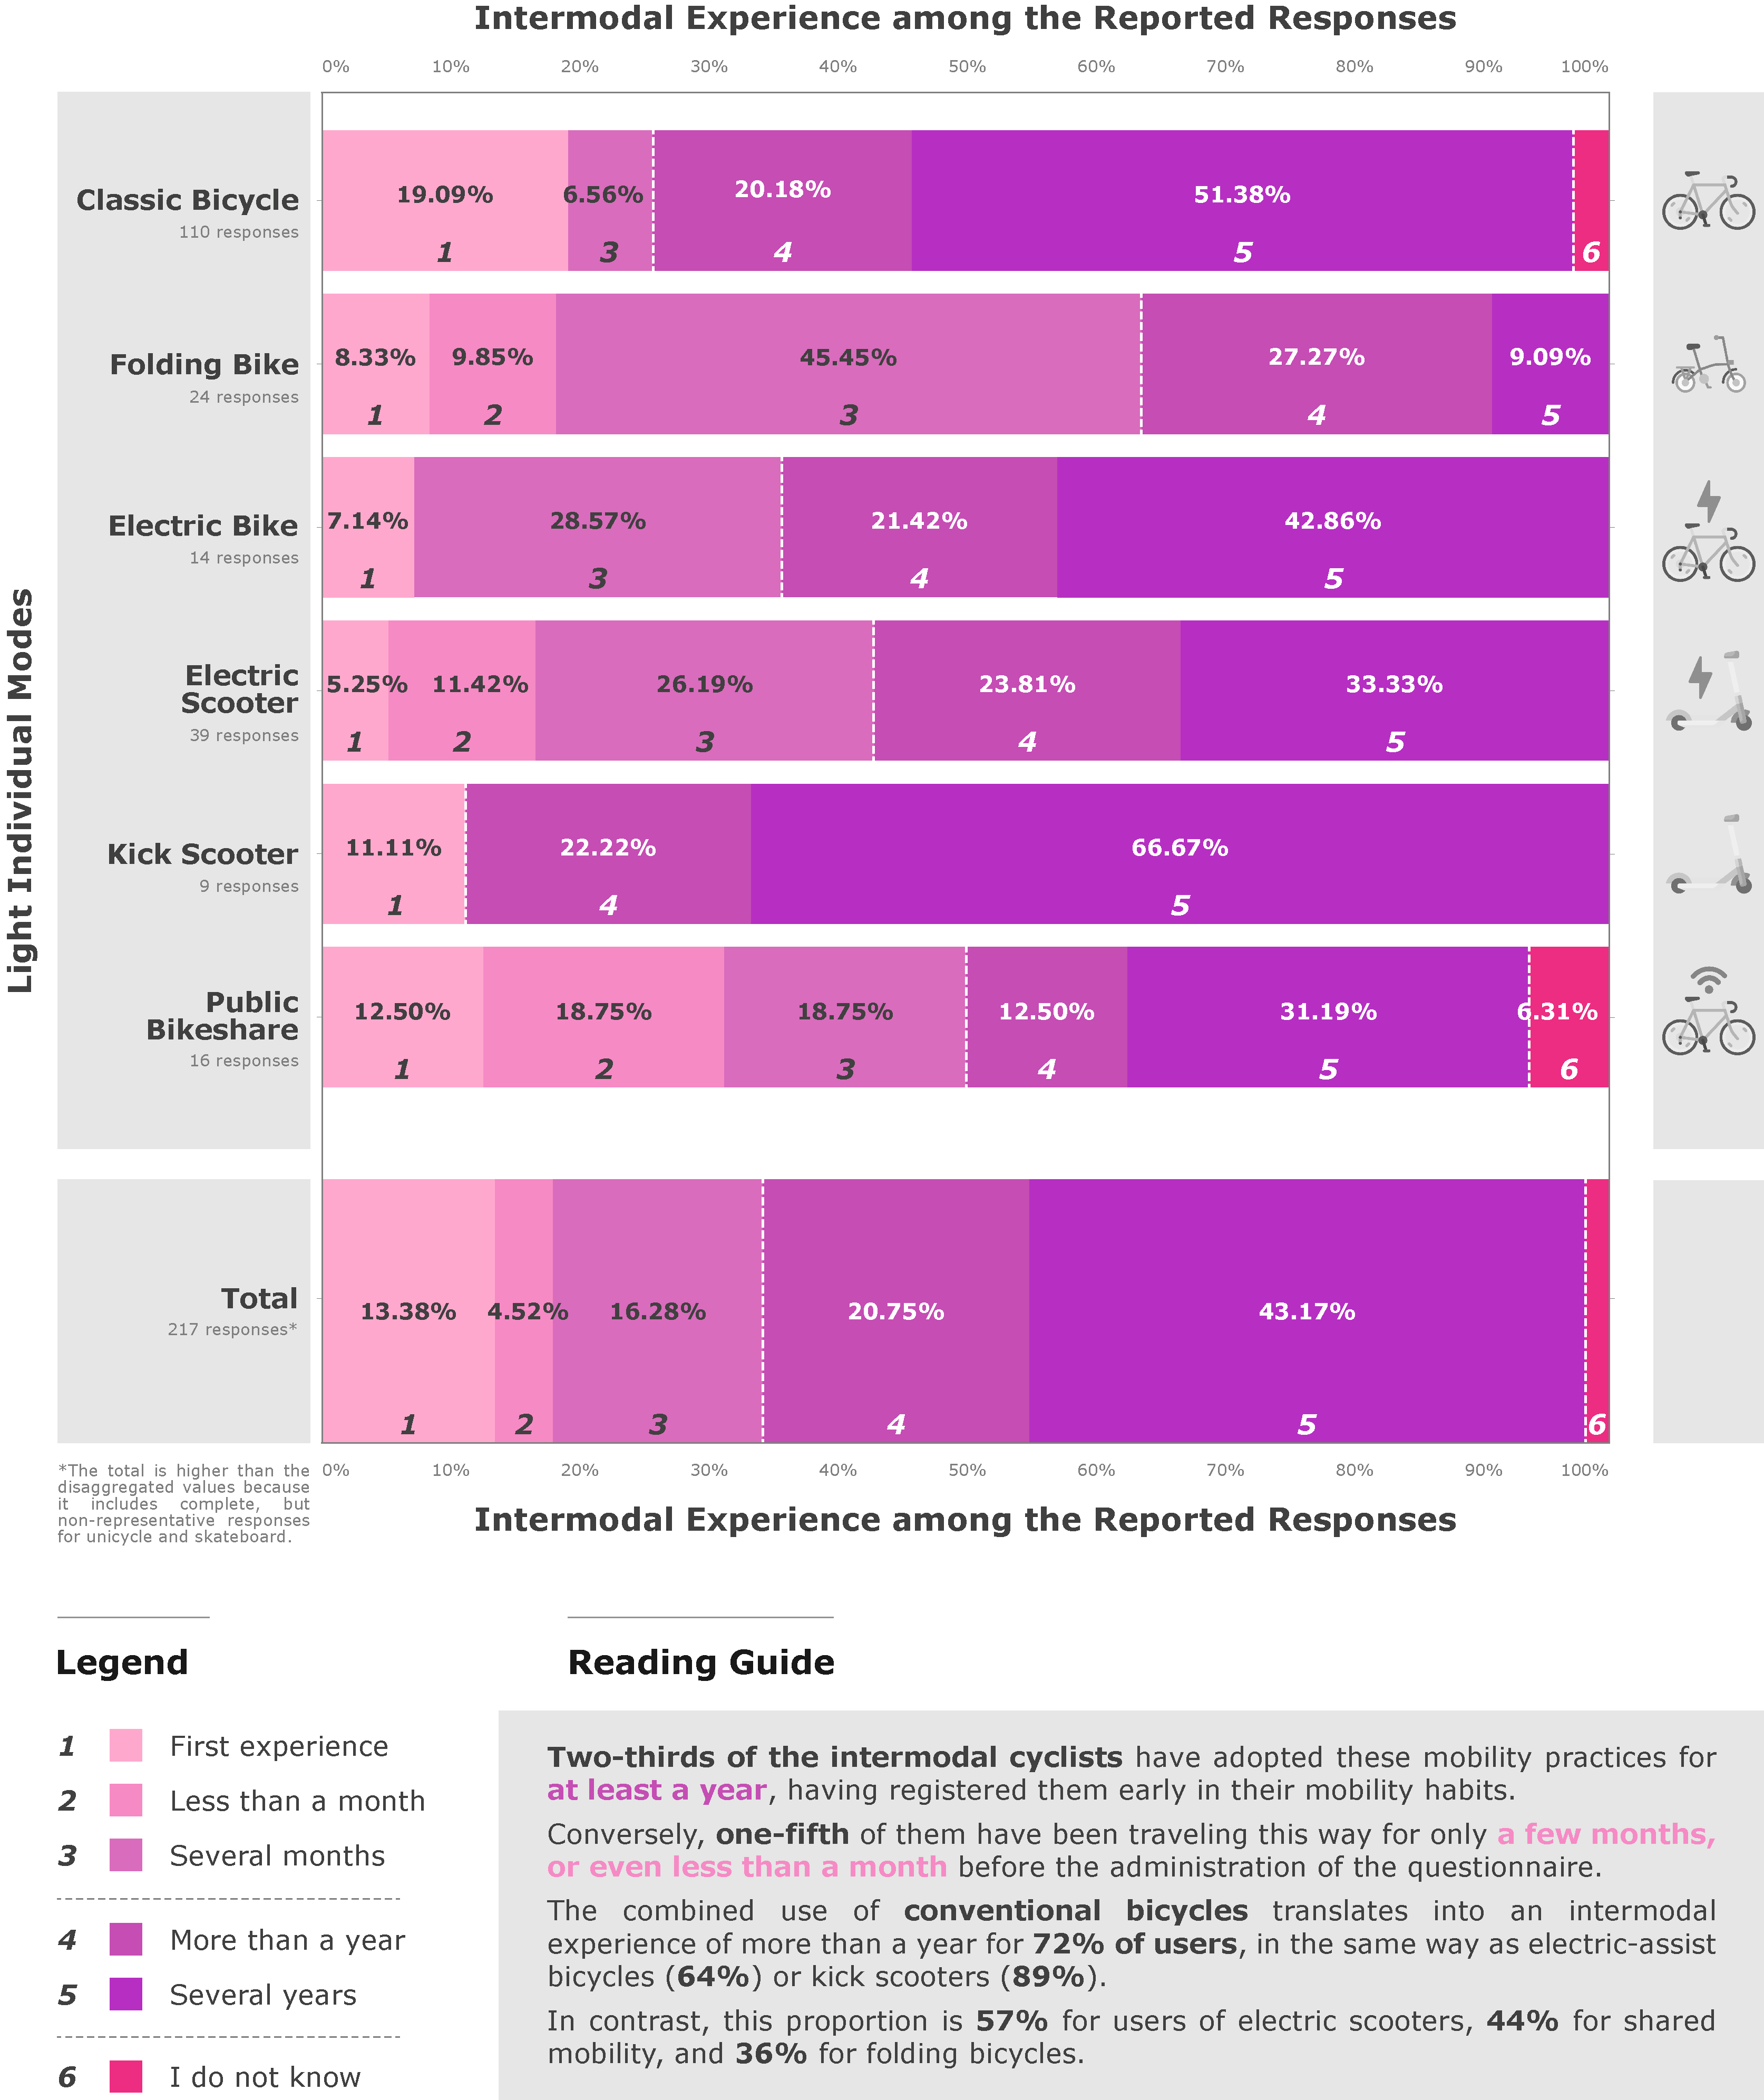
\includegraphics[width=1\columnwidth]{src/Figures/Chap-4/EN_Experience_intermodale.pdf}}
    \vspace{5pt}
    \begin{flushright}\scriptsize{
    Author: \textcolor{blue}{Dylan Moinse (2023)}
    }\end{flushright}
\end{figure}

% Résultats par mode expérience intermodale
By refining the analysis of the survey based on the different vehicles that make up the corpus of light individual mobility, it appears that mechanical scooters and conventional bicycles are integrated into established intermodal configurations, with more than three-quarters of users practicing them for at least one year. In contrast, the \acrfull{e-Bike}, \acrshort{PeS}, shared mobility systems, and folding bicycles show more recent adoption among users: a third, or even half, of them started using them only a few months ago. As a result, it is reasonable to deduce that conventional bicycles, on the one hand, represent a mode of transport deeply rooted in intermodal practices, traditionally associated with the bicycle and public transport combination. On the other hand, variations of the bicycle, such as folding and electric bicycles, reflect a recent resurgence, while the \acrshort{PeS}, \acrshort{PBS}, \acrshort{DBS}, and \acrshort{DESS} are in a growth phase.%%Translated%%

% Littérature expérience intermodale - vélo
The comparison with the current state of knowledge reveals that the combination of bicycles with public transport has generated significant interest, particularly between 2005 and 2015. These intermodal practices indeed present potential for modal share growth, associated with a high level of user retention over time. Regarding conventional bicycles, there has been a noticeable increase in their use as a transfer mode to and from Dutch train stations, rising from 35\% (access) and 10\% (egress) in 2000 \textcolor{blue}{\autocite[73]{rietveld_accessibility_2000}}\index{Rietveld, Piet|pagebf} to 43\% (access) and 14\% (egress) in 2016 \textcolor{blue}{\autocite[456-457]{jonkeren_bicycle-train_2021}}\index{Jonkeren, Olaf|pagebf}\index{Kager, Roland|pagebf}\index{Harms, Lucas|pagebf}\index{te Brömmelstroet, Marco|pagebf}. In the United States, the intermodal use of bicycles has increased from 0.0\% to 0.6\% \textcolor{blue}{\autocite[101]{wang_bicycle-transit_2013}}\index{Wang, Rui|pagebf}\index{Liu, Chen|pagebf}, particularly in densely populated regions \textcolor{blue}{\autocite[107]{wang_bicycle-transit_2013}}\index{Wang, Rui|pagebf}\index{Liu, Chen|pagebf}. These data highlight the upward trend in the modal share of bicycles, while also emphasizing the existence of a community of travelers who remain loyal to these intermodal practices. Indeed, according to \textcolor{blue}{Christian} \textcolor{blue}{\textcite[18]{gioria_etude_2016}}\index{Gioria, Christian|pagebf}, 68\% of bicycle locker users at train stations in France have been using this service for more than a year, and 44\% for more than two years.%%Translated%%

% Littérature expérience intermodale - micro-mobilité
The notion of emergence, as described by \textcolor{blue}{\textcite[4]{kostrzewska_towards_2017}}\index{Kostrzewska, Małgorzata|pagebf}\index{Macikowski, Bartosz|pagebf}, suggests that the integration of micromobility is particularly promising in terms of modal adoption growth. In France, the report from \textcolor{blue}{\textcite[10]{ademe_observatoire_2017}}\index{ADEME@\textsl{ADEME}|pagebf} indicates that the market for modes connecting to transport hubs is marked by significant penetration of \Commas{urban glide} devices, whose share doubled between 2014 and 2017, with a modal share of micromobility reaching 6\%. The FP2M Barometer confirms this trend, recording a 34\% increase in sales of \acrshort{PeS} between 2019 and 2020, representing 640,000 units sold, compared to only 100,000 in 2017 \textcolor{blue}{\autocite[2]{fp2m_barometre_2021}}\index{FP2M@\textsl{FP2M}|pagebf}\index{SML@\textsl{SML}|pagebf}. The study conducted by the \textcolor{blue}{\textcite[11]{smart_mobility_lab_usages_2020}}\index{Smart Mobility Lab@\textsl{Smart Mobility Lab}|pagebf} reports that 73\% of monomodal \acrshort{PeS} users started using them less than a year ago, with 43\% having adopted them less than six months ago. This evolution is even more notable as it was catalyzed by the COVID-19 health crisis, which prompted 27\% of mobile individuals surveyed to modify their travel habits, with 29\% adopting a bicycle or \acrshort{e-Bike}, and 16\% opting for a micromobility option \textcolor{blue}{\autocite[16]{smart_mobility_lab_usages_2020}}\index{Smart Mobility Lab@\textsl{Smart Mobility Lab}|pagebf}.%%Translated%%

% Transition
It is essential, when analyzing the modal shares of light individual mobility, to recognize the diverse urban contexts in which train stations are located. The following section demonstrates how the specific characteristics of urban and peri-urban areas influence intermodal practices, given that urban centers, often better equipped in terms of mobility services, may exhibit mobility dynamics distinct from those in peri-urban areas, where transport infrastructure may be less diversified and the distances to travel greater.%%Translated%%

% 4.1.1.3.
\needspace{1\baselineskip} % Réserve de l'espace
\subsubsection*{A Relevant Mode of Transport for Feeder Stations to Urban Hubs
    \label{chap4:part-modale-gares-centre-periurbain}
    }

% Introduction
An exercise in contextualizing the studied train stations was undertaken to examine the modal shares of light individual mobility within modal chains. This study highlights a characteristic spatial distribution of these intermodal practices, marked by a relative concentration depending on the territorial polarity in which the station is located. This subsection thus aims to capture the geographical variations of such intermodal trips, emphasizing the importance of urban contexts in the adoption and integration of light mobility within the rail network.%%Translated%%

    % Tableau Typologie des gares HdF
% Table Typology of Stations in Hauts-de-France  
%%Translated%%  
    \begin{table}[h!]  
    \centering  
    \renewcommand{\arraystretch}{1.5}  
    \resizebox{\columnwidth}{!}{  
    \begin{tabular}{p{0.27\columnwidth}p{0.13\columnwidth}p{0.60\columnwidth}}  
        %\hline  
    \rule{0pt}{15pt} \small{\textbf{\textcolor{blue}{Station or Halt}}} & \small{\textbf{\textcolor{blue}{\acrshort{DRG}}}} & \small{\textbf{\textcolor{blue}{Contextualization of the Class}}}\\  
        \hline  
\small{Creil} & \multirow{2}{*}{\small{Profile~\(a\)}} & \multirow{2}{*}{\small{\textsl{Stations of regional hubs}}}\\  
    \small{Lille Flandres} & & \\  
        \hdashline  
\small{Armentières} & \multirow{3}{*}{\small{Profile~\(b\)}} & \multirow{3}{*}{\small{\textsl{Stations of intermediate hubs}}}\\  
    \small{Béthune} & & \\  
    \small{Dunkerque} & & \\  
        \hdashline 
\small{Le Poirier Université} & \multirow{4}{*}{\small{Profile~\(c\)}} & \multirow{4}{*}{\small{\textsl{Stations feeding into urban centers}}}\\
\small{Lesquin} & & \\  
\small{Lille CHR} & & \\  
\small{Vis-à-Marles} & & \\  
        \hline  
        \end{tabular}}  
    \caption{Reuse of the \Commas{Segment DRG} reference applied to the nine stations explored in the Hauts-de-France region.}  
    \label{table-chap4:typologie-gares-hdf}  
        \vspace{5pt}  
        \begin{flushleft}\scriptsize{  
        \textcolor{blue}{Reading Guide~:} This table applies the segment typology to the nine stations in the Hauts-de-France region explored in our investigation, classifying them into three distinct profiles: profiles \(a\), \(b\), and \(c\).  
        }\end{flushleft}  
        \begin{flushright}\scriptsize  
        Datasets~: \textcolor{blue}{\textcite{sncf_gares__connexions_gares_2024}}\index{SNCF Gares \& Connexions@\textsl{SNCF Gares \& Connexions}|pagebf}  
        \\
        Author~: \textcolor{blue}{Dylan Moinse (2022)}  
        \end{flushright}  
        \end{table}%%Rédigé%%

% Méthodologie
Our analytical approach, based on the station typology established by \textcolor{blue}{\textcite{sncf_gares__connexions_gares_2024}}\index{SNCF Gares \& Connexions@\textsl{SNCF Gares \& Connexions}|pagebf}, allowed us to refine the characterization of the modal shares of light individual mobility for access to and from the various stations in the region. The data collected during the quantitative observation sessions were systematically cross-referenced with the station classification called \Commas{Segment \acrfull{DRG}}\footnote{~
    The \Commas{Segment \acrshort{DRG}} reference produced by the Strategy Directorate \textcolor{blue}{\textcite{sncf_gares__connexions_gares_2024}} defines three distinct categories of stations, each reflecting a scale of interest and annual traffic. This classification system, primarily based on station traffic volumes, evaluates 3,009 stations across France, including 265 in the Hauts-de-France region. These profiles are distributed as follows: 
    \begin{customitemize}
    \item Class~\(a\), referring to \Commas{national interest passenger stations}, includes stations with high traffic, having an annual traffic of more than 250,000 passengers. At the national level, 102 stations are classified in this category, with 8 located in the Hauts-de-France region;
    \item Class~\(b\), corresponding to \Commas{regional interest passenger stations}, includes stations with an annual traffic between 100,000 and 250,000 passengers. This category comprises 928 stations, with 62 in the Hauts-de-France region;
    \item Class~\(c\), including \Commas{local interest passenger stations}, consists of less frequented stations with an annual flow of fewer than 100,000 passengers. Nationally, 1,978 stations belong to this class, with 195 in the Hauts-de-France region.
    \end{customitemize}
} (see \hyperref[table-chap4:typologie-gares-hdf]{Table~\ref{table-chap4:typologie-gares-hdf}}, page~\pageref{table-chap4:typologie-gares-hdf}). The use of this framework led us to interpret the categories from the \Commas{Segment \acrshort{DRG}} reference in the context of the nine stations studied:
    \begin{customitemize}
\item Regional hub stations (\(a\)), located at the heart of urban centers, comprising two main stations;
\item Intermediate hub stations (\(b\)), located in medium-sized cities, comprising three stations;
\item Feeder stations to regional centers (\(c\)), located on the outskirts of urban centers, comprising four stations.
    \end{customitemize}%%Translated%%

% Observation répartition géographique
The analysis of the modal shares of light individual mobility onboard different stations, based on their profile, reveals a heterogeneous distribution corresponding to the various urban and peri-urban contexts of the examined stop points. While central stations such as Lille Flandres and Creil concentrate a significant number of intermodal cyclists, with 387 individuals observed, representing 37\% of the sub-sample, it is interesting to note that peri-urban areas served by some of the surveyed stations show a higher modal share of light individual mobility relative to their total traffic, provided there is an adequate level of service (see \hyperref[fig-chap4:part-modale-urbain-periurbain]{Figure~\ref{fig-chap4:part-modale-urbain-periurbain}}, page~\pageref{fig-chap4:part-modale-urbain-periurbain}). In detail, class~\(a\), which includes the two aforementioned stations, records a proportion of intermodal users of 5\% (out of 7,995 observations). In contrast, class~\(b\), which includes the stations of Armentières, Béthune, and Dunkirk, shows a modal share of 7\% (out of 5,826 observations). This trend is even more pronounced in class~\(c\), which includes the stations of Lille CHR, Le Poirier Université, Lesquin, and Vis-à-Marles, with a modal share of 14\% (out of 1,617 observations).%%Translated%%

% Observation répartition géographique détails modes 1
By refining this study to the different components of light individual mobility, we can observe a certain consistency in the geographical distribution of the observed modal shares. The \hyperref[fig-chap4:part-modale-urbain-periurbain]{Figure~\ref{fig-chap4:part-modale-urbain-periurbain}} (page~\pageref{fig-chap4:part-modale-urbain-periurbain}) highlights a steady increase in modal shares as we move towards the third class of the typology, except for the Vis-à-Marles stop. This phenomenon indicates a preferred adoption of light individual mobility as a transfer mode in peri-urban contexts:
    \begin{customitemize}
\item For conventional bicycles, a gradual increase in modal share is identified across the different classes, ranging from 1.55\% for class~\(a\) (124 observations), to 2.18\% for class~\(b\) (127 observations), and 4.83\% for class~\(c\) (78 observations);
\item For folding bicycles, the modal shares are 0.56\% for class~\(a\) (45 observations), 0.81\% for class~\(b\) (47 observations), and 1.92\% for class~\(c\) (31 observations);
\item For the \acrshort{PeS}, the shares reach 2.26\% for class~\(a\) (171 observations), 3.16\% for class~\(b\) (184 observations), and 5.89\% for class~\(c\) (95 observations);
\item Mechanical scooters show a distribution of 0.43\% for class~\(a\) (34 observations), 0.96\% for class~\(b\) (56 observations), and 0.87\% for class~\(c\) (14 observations);
\item For other forms of \acrshort{PMD}, the shares are 0.15\% for class~\(a\) (12 observations), 0.24\% for class~\(b\) (14 observations), and 0.12\% for class~\(c\) (2 observations).
    \end{customitemize}%%Translated%%

% Observation répartition géographique détails modes 2
However, some exceptions temper this general trend. For example, the Lille CHR stop shows a low modal share for mechanical scooters. This particularity can be explained by the urban forms of the surrounding area, characterized by low permeability in the urban fabric and the presence of large parcels such as the \acrfull{CHU} of Lille, which limits the effectiveness of this muscle-powered mode of transport. Similarly, the intermodal use of \acrshort{PMD}, excluding the \acrshort{PeS} and including modes such as the skateboard, unicycle, and segway, does not seem to align with the observed trend, likely due to a sample size that is too small to provide a reliable statistical representation.%%Translated%%

% Figure Part modale périurbain
\begin{figure}[h!]\vspace*{4pt}
    \caption{An Intermodal Use of Light Individual Mobility Stimulated in Peri-Urban Areas.}
    \label{fig-chap4:part-modale-urbain-periurbain}
    \centerline{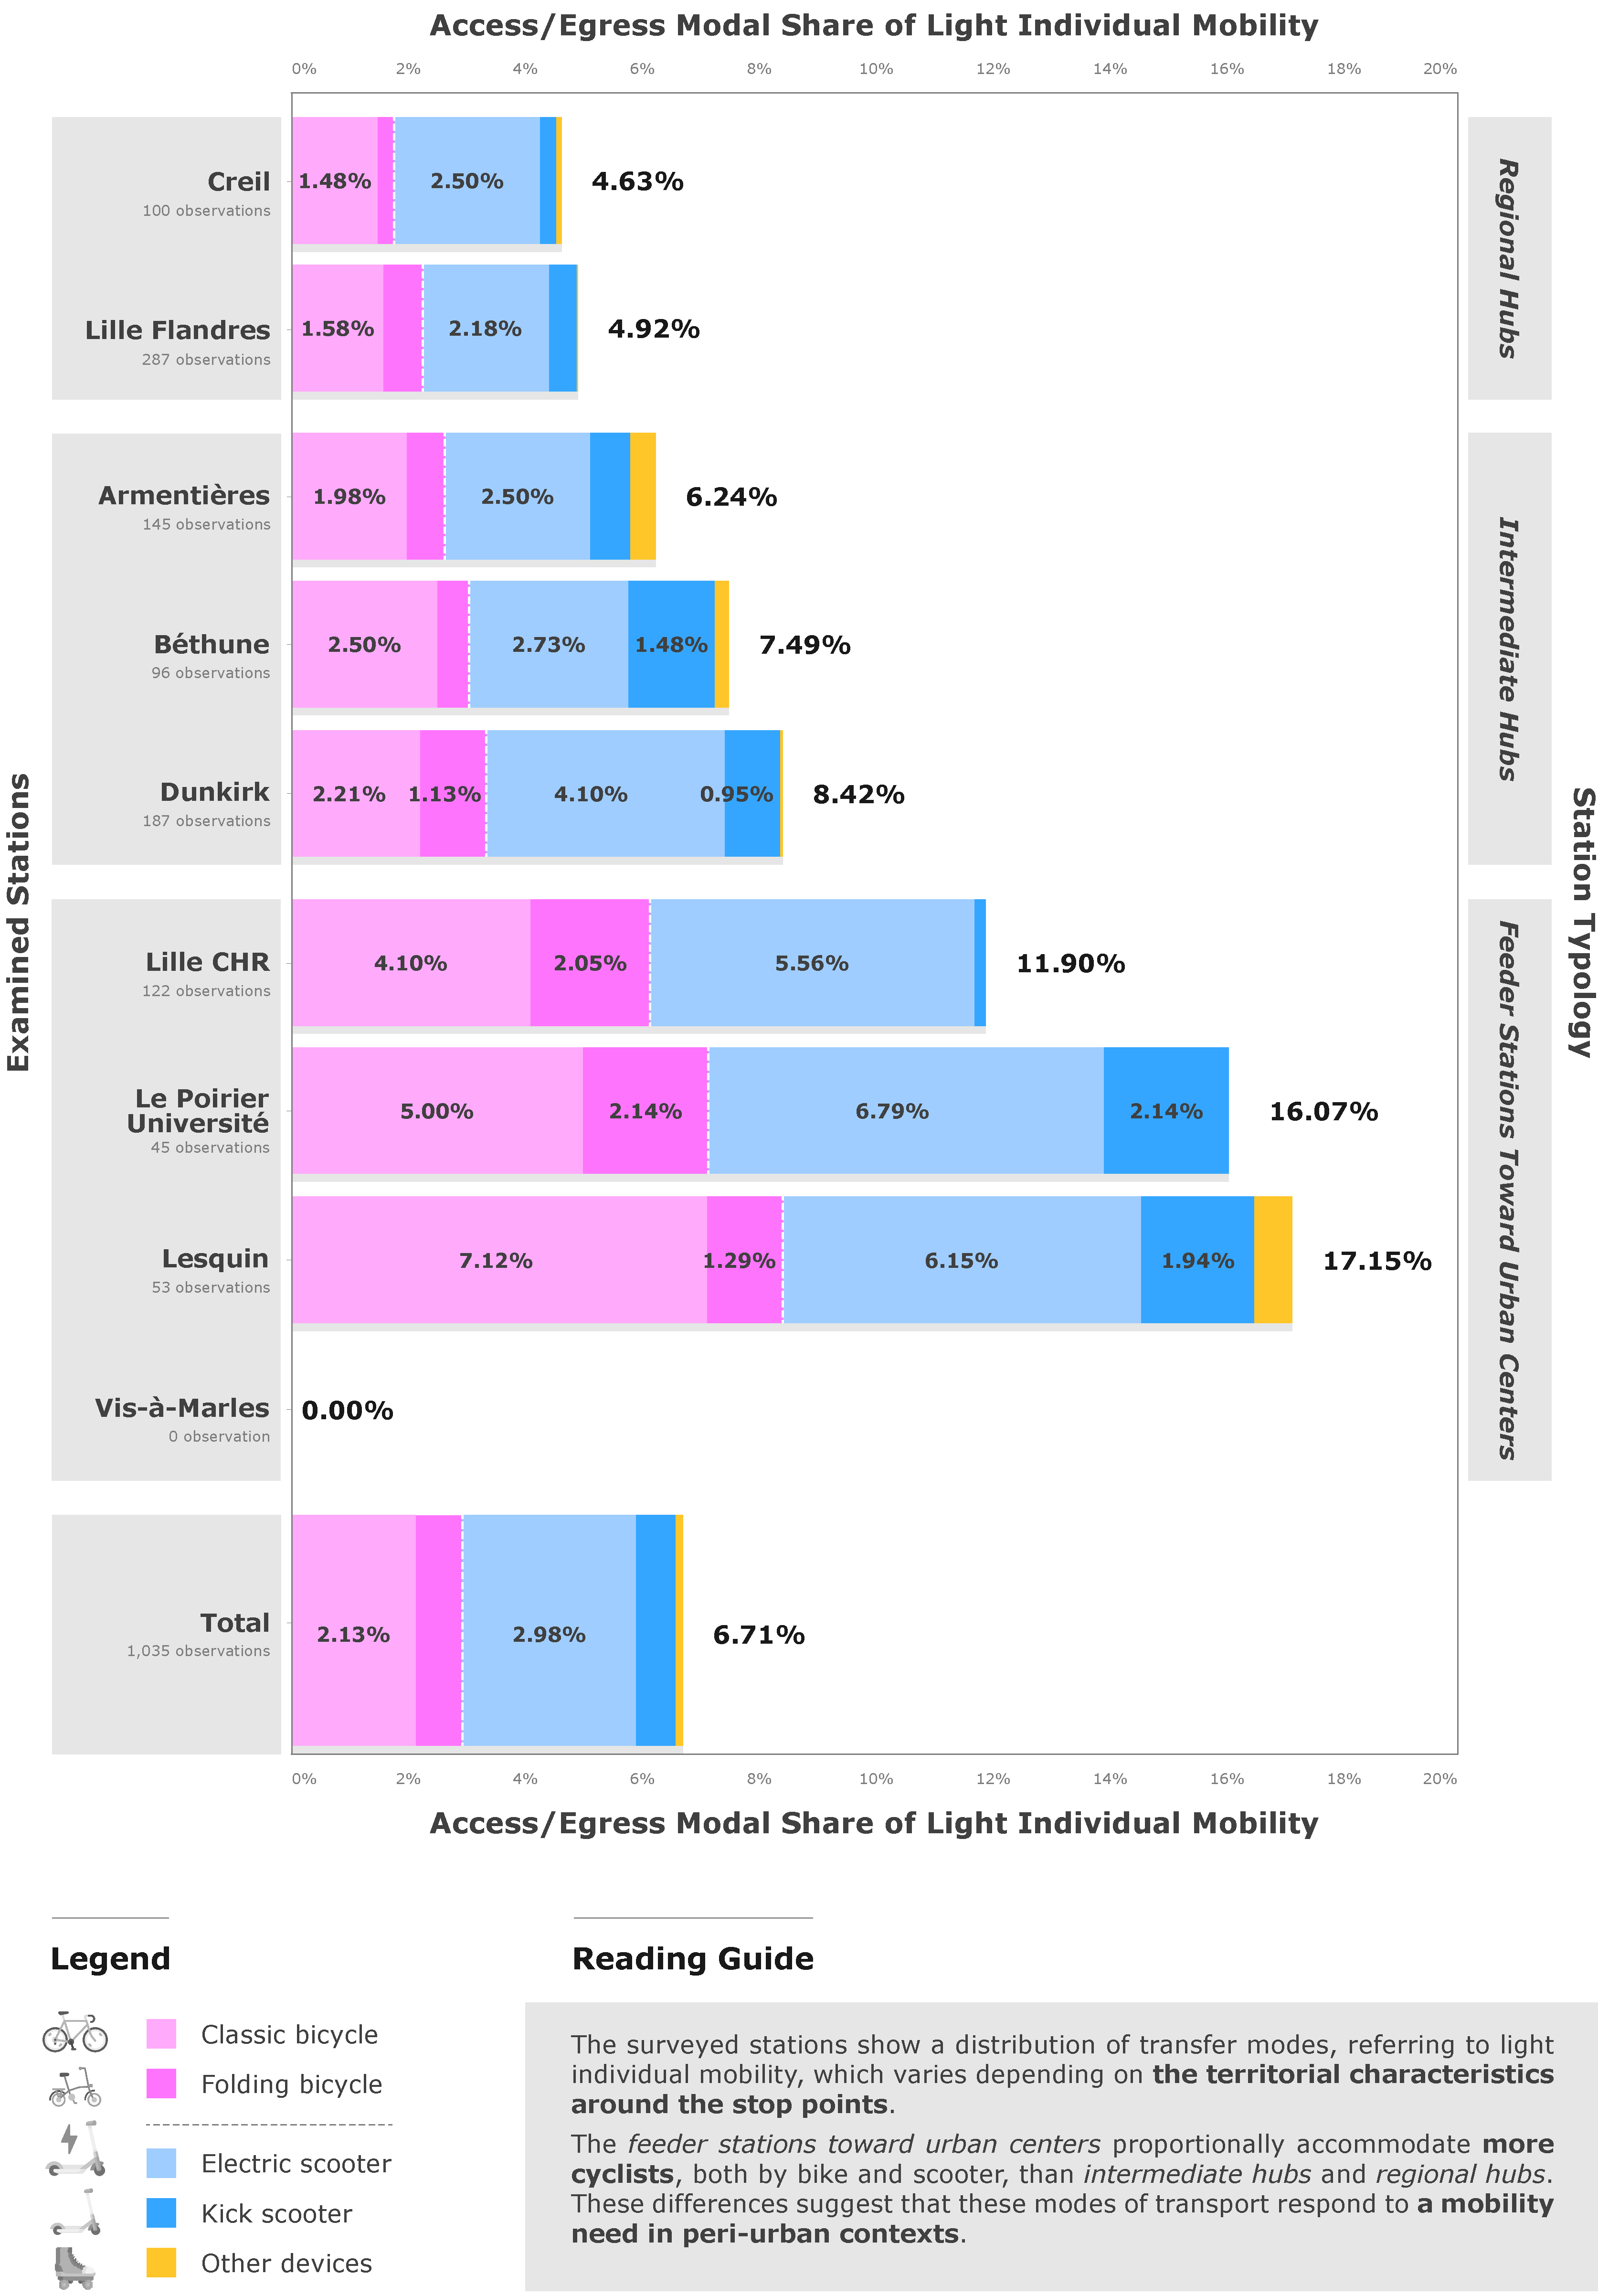
\includegraphics[width=1\columnwidth]{src/Figures/Chap-4/EN_Part_modale_MIL_gares.pdf}}
    \vspace{5pt}
    \begin{flushright}\scriptsize{
    Author: \textcolor{blue}{Dylan Moinse (2023)}
    }\end{flushright}
\end{figure}

% Complément questionnaire flux OD
By analyzing the origin and destination flows collected in the survey, this geostatistical analysis seeks to deepen the understanding of the types of territories that light individual mobility combined with public transport tends to connect. While the quantitative observation highlights the strategic role of second-tier stations in the regional rail network, the survey responses emphasize a high density of flows to the most frequented stations. The spatial evaluation of the 99 intermodal trips projected in the 9 studied stations reveals a majority of trips by bicycle or micromobility connecting a class~\(a\) station to a class~\(b\) station, and vice versa (60 flows). Next are the trips between stations of the same type, notably those of class~\(b\) (15 flows) and class~\(a\) (10 flows). Interactions involving a class~\(c\) station are less frequent, with few trips between class~\(a\) and class~\(c\) stations (8 flows), between class~\(b\) and class~\(c\) stations (5 flows), and between class~\(c\) stations (1 flow).%%Translated%%

% Aires attraction
However, by cross-referencing feeder and dispersal routes with the \acrfull{UAA} zoning produced by \textcolor{blue}{\textcite{insee_nouveau_2020}}\index{Insee@\textsl{Insee}|pagebf}\footnote{~
    The new \acrfull{UAA} zoning consists of its core, with its most populous municipality referred to as the \Commas{central municipality}, and its surrounding area, the crown \textcolor{blue}{\autocite{insee_nouveau_2020}}. The crowns group municipalities where at least 15\% of the active residents work within the cores or multi-core areas. 
    In the Hauts-de-France region, 65 urban attraction areas are recorded, 7 of which are in neighboring regions, and 2 others extend into Belgium, covering 83\% of the region's municipalities and 95\% of the population \textcolor{blue}{\autocite{insee_plus_2020}}.
}, we can deduce that, among the 78 intermodal trips associated with a class~\(a\) station, 42 of them involve an origin and/or destination located within a \Commas{large core crown} or \Commas{medium cores}. This finding suggests that, while the intermodal adoption of light individual mobility is focused on the most attractive stations, half of these trips occur, at the destination, in less densely populated areas.%%Translated%%

% Littérature urbain - périurbain
From the perspective of existing documentation on the topic, it is widely accepted in a significant portion of the literature that urban and central areas are particularly favorable to the intermodal adoption of light individual mobility. However, our research presents contrary results regarding the analyzed modal shares, offering new perspectives on the underexplored case of micromobility. A survey conducted by the consulting firm \textcolor{blue}{\textcite[18]{enov_enquete_2021}}\index{Enov@\textsl{Enov}|pagebf} in six major French train stations—Bercy, Gare de l'Est, Gare de Lyon, Lille Flandres, Lille Europe, and Rouen Rive Droite—attributes an average modal share of 2\% for bicycles and 2\% for micromobility, whether personal or shared. These results support the hypothesis of a less visible distribution of light individual mobility transfer modes in central stations. In a comparative study between the Netherlands, Germany, and the United Kingdom, \textcolor{blue}{\textcite[291]{martens_bicycle_2004}}\index{Martens, Karel|pagebf}, as well as \textcolor{blue}{\textcite[25]{halldorsdottir_home-end_2017}}\index{Halldórsdóttir, Katrín|pagebf}\index{Nielsen, Otto Anker|pagebf}\index{Prato, Carlo Giacomo|pagebf} in the case study of Copenhagen, demonstrated that the combination of bicycles and public transport is more frequent in peripheral areas. Bicycles are perceived as a strategic element for extending the reach of rail services in peri-urban and rural areas \textcolor{blue}{\autocite[86]{zuo_incorporating_2021}}\index{Zuo, Ting|pagebf}\index{Wei, Heng|pagebf}\index{Chen, Na|pagebf}. These observations suggest that the use of light individual mobility in possession is favored in a peri-urban context \textcolor{blue}{\autocite[38]{stransky_periurbain_2019}}\index{Stransky, Vaclav|pagebf}, and is therefore not reserved for the central areas of urban agglomerations as claimed by part of the literature.%%Translated%%

% Transition
Having examined the strategic role of bicycles and micromobility in stations acting as feeder points to urban centers, it is essential to recognize the extent of their modal adoption across the different observed modal chaining schemes, particularly in terms of vehicle boarding and parking. At this stage of the analysis, it is legitimate to question the role played by bicycles and micromobility in the modal chain. More specifically, we are led to determine whether these modes of transport are primarily used during the access or egress stages. The following section explores more specifically the feeder and dispersal stages of intermodal practices specific to each mode of transport.%%Translated%%

% 4.1.1.4.
\needspace{1\baselineskip} % Réserve de l'espace
\subsubsection*{A Clear Adoption in Both Access and Egress Stages
    \label{chap4:rabattement-diffusion}
    }

% Questionnaire access/egress modes
The survey provides an additional level of detail regarding the different phases of each trip that integrates light individual mobility and the public transport system. Generally, it appears that bicycles and micromobility, whether onboard or not, are used in almost identical proportions for the feeder and dispersal stages, reaching 78\% and 79\% respectively out of a total of 217 intermodal trips, although variations exist depending on the type of vehicle involved. The \hyperref[table-chap4:part-modale-acces-diffusion-urbain-periurbain]{Table~\ref{table-chap4:part-modale-acces-diffusion-urbain-periurbain}} (page~\pageref{table-chap4:part-modale-acces-diffusion-urbain-periurbain}) shows that users of conventional bicycles and \acrshort{e-Bike} particularly favor the access stage to public transport hubs (for 110 and 14 trips). In contrast, folding bicycles, \acrshort{PeS}, mechanical scooters, as well as shared bike and scooter systems tend to favor the egress stage from these hubs (for 24, 39, 9, and 16 trips). By comparison, combined walking is used much more frequently during the dispersal stage (for 47 trips).%%Translated%%

% Confrontation access/egress modes
Statistical analyses of user mobility behaviors depict bicycles, both muscle-powered and electric, as an appropriate mode of transport for the \Commas{first miles}, often combined with walking during the dispersal stage. In parallel, folding bicycles and micromobility, notably represented by scooters, redefine the challenge of the \Commas{first and last miles} by addressing the needs related to the \Commas{last miles}. These light vehicles tend to be frequently combined with car use, whether as a driver or passenger, as well as with urban public transport networks for the feeder stage. This diversity of intermodal practices between these two categories of vehicles is partly due to the comparative advantages offered by folding bicycles and scooters. Indeed, their compactness and lightness make it easier to board them onto other vehicles, a context in which the use of conventional or electric bicycles proves less practical.%%Translated%%

    % Tableau Part modale intermodale - modes de transfert
% Table Modal Share of Intermodal Light Individual Mobility - Transfer Modes
%%Rédigé%%
    \begin{table}[h!]
    \centering
    \renewcommand{\arraystretch}{1.5}
    \resizebox{\columnwidth}{!}{
    \begin{tabular}{p{0.4\columnwidth}p{0.18\columnwidth}p{0.14\columnwidth}p{0.14\columnwidth}p{0.14\columnwidth}}
        %\hline
    \rule{0pt}{15pt} \small{\textbf{\textcolor{blue}{Type of Vehicle}}} & \small{\textbf{\textcolor{blue}{Access}}} & \small{\textbf{\textcolor{blue}{Peri-urban}}} & \small{\textbf{\textcolor{blue}{Egress}}} & \small{\textbf{\textcolor{blue}{Peri-urban}}}\\
        \hline
\small{\textbf{All types of light individual mobility combined}} & \multirow{1.5}{*}{\small{\textbf{78.34\%}}} & \multirow{1.5}{*}{\small{\textbf{31.86\%}}} & \multirow{1.5}{*}{\small{\textbf{78.80\%}}} & \multirow{1.5}{*}{\small{\textbf{20.59\%}}}\\
        \hdashline
\small{Conventional bicycle} & \small{80.51\%} & \small{34.58\%} & \small{65.25\%} & \small{20.56\%}\\
\small{Electric bicycle (\acrshort{e-Bike})} & \small{76.92\%} & \small{60.00\%} & \small{61.54\%} & \small{20.00\%}\\
\small{Folding bicycle} & \small{80.95\%} & \small{21.74\%} & \small{100.00\%} & \small{26.09\%}\\
\small{Electric scooter (\acrshort{PeS})} & \small{80.43\%} & \small{38.46\%} & \small{100.00\%} & \small{25.64\%}\\
\small{Mechanical scooter} & \small{77.78\%} & \small{20.00\%} & \small{100.00\%} & \small{20.00\%}\\
\small{Shared mobility} & \small{40.00\%} & \small{0.00\%} & \small{70.00\%} & \small{0.00\%}\\
        \hdashline
\small{Combined walking} & \small{36.17\%} & \small{17.24\%} & \small{63.83\%} & \small{10.34\%}\\
        \hline
        \end{tabular}}
    \caption{Intermodal use of light individual mobility for pre-transport and post-transport towards and from suburban areas.}
    \label{table-chap4:part-modale-acces-diffusion-urbain-periurbain}
        \vspace{5pt}
        \begin{flushleft}\scriptsize{
        \textcolor{blue}{Reading Guide:} Among users combining light individual mobility with the public transport system and who reported their journey in the survey, 78\% travel with a light vehicle in access and 32\% originate from suburban areas, while 79\% use it in egress and 21\% have a destination in suburban areas.
        }\end{flushleft}
        \begin{flushright}\scriptsize
        Author: \textcolor{blue}{Dylan Moinse (2023)}
        \end{flushright}
        \end{table}%%Rédigé%%

% Access/egress et urbain/périurbain
Unlike the traditional triptych composed of bicycles, public transport, and combined walking, the \acrshort{PeS} and folding bicycles offer their users the ability to reach more distant destinations once they have exited the public transport station. This capability theoretically extends accessibility to certain peri-urban areas, as shown in the \hyperref[table-chap4:part-modale-acces-diffusion-urbain-periurbain]{Table~\ref{table-chap4:part-modale-acces-diffusion-urbain-periurbain}} (page~\pageref{table-chap4:part-modale-acces-diffusion-urbain-periurbain}). Indeed, 38\% of travelers using \acrshort{PeS} and 26\% of folding bicycle travelers start or end their trip in peri-urban areas. These proportions are comparable to those observed for conventional bicycles for the \Commas{first miles}, but exceed them during the dispersal phase.%%Translated%%

% Discussion
This subsection has demonstrated that light individual mobility is frequently used as a transfer mode, effectively complementing the public transport network. The rise of the \acrshort{PeS}, electric-assist folding bicycles, as well as shared bicycle and micromobility services, appears to have significantly boosted its modal share. The intermodal use of light individual mobility is employed both for the feeder and dispersal stages, with a growing adoption of folding vehicles. While the number of users is higher in urban centers, their presence is proportionally more marked in peri-urban areas served by stations offering a certain level of service. Furthermore, it was observed that these modes of transport are primarily concentrated in the most central stations, but then extend to more distant areas from the urban hubs. This observation suggests that intermodal cyclists are willing to prioritize connections to well-served stations and cover longer distances to reach peri-urban areas. This hypothesis will be explored in the \hyperref[chap5:detours-pauses-optimisation]{section on optimizing movement through detours} (page~\pageref{chap5:detours-pauses-optimisation}) in \hyperref[chap5:titre]{Chapter~5} (page~\pageref{chap5:titre}).%%Translated%%

% Transition
The emergence of new forms of mobility, combined with the return of bicycles as part of light individual mobility, seems to significantly increase the share of intermodal travelers at train stations, with an estimated increase ranging from a quarter to half of the initial proportion. However, this statistical interpretation needs to be verified, particularly by examining the potential modal substitution effect induced by these newly adopted vehicles. The underlying question is to determine to what extent micromobility simply substitutes for pre-existing intermodal practices, where bicycles were combined with rail, or if it truly leads to a net increase in the number of users opting for intermodal combinations. More broadly, the following subsection aims to better understand the mobility behaviors of intermodal cyclists.%%Translated%%

% 4.2.1.
\needspace{1\baselineskip} % Réserve de l'espace
\subsection{Mobility Behaviors
    \label{chap4:comportements-mobilite}
    }

% Introduction
After validating the first hypothesis that the integration of light individual mobility into public transport networks is in an emerging phase, we now turn to exploring the interactions with rail services. The focus is now on analyzing the impact and opportunities that these intermodal practices present for public transport systems. The use of data collected through the online-administered survey has provided an initial overall characterization of mobility behaviors in relation to intermodal practices at train stations. In this regard, a specific section of the survey was dedicated to examining respondents' habits regarding the combined use of these modes of transport, their travel motives, intermodal experience, and the underlying motivations for such mobility practices.%%Translated%%

% 4.2.1.1.
\needspace{1\baselineskip} % Réserve de l'espace
\subsubsection*{Intermodal Trips Embedded in Daily Mobility
    \label{chap4:frequence-motif-experience}
    }

% Fréquence - général
The intermodal use of light individual mobility appears to primarily serve frequent trips, typically commuting, as shown in the \hyperref[fig-chap4:frequence-modes]{Figure~\ref{fig-chap4:frequence-modes}} (page~\pageref{fig-chap4:frequence-modes}). Of 100 intermodal travelers using light individual mobility, 53 adopt this practice almost daily (\Commas{more than one trip per day} or \Commas{several trips per week}, 116 responses), and 8 on a regular basis (\Commas{one trip per week}, 17 responses). The other frequency segments are distributed as follows: 13 use it occasionally (\Commas{several times a month} or \Commas{at least once a month}, 28 responses), 12 maintain a rare frequency (\Commas{several times a year} or \Commas{at least once a year}, 26 responses), and 13 respondents report that their participation in the survey coincides with their first intermodal experience (\Commas{first use}, 28 responses).%%Translated%%

% Figure fréquence modes
\begin{figure}[h!]\vspace*{4pt}
    \caption{Frequency of Intermodal Use of Light Individual Mobility.}
    \label{fig-chap4:frequence-modes}
    \centerline{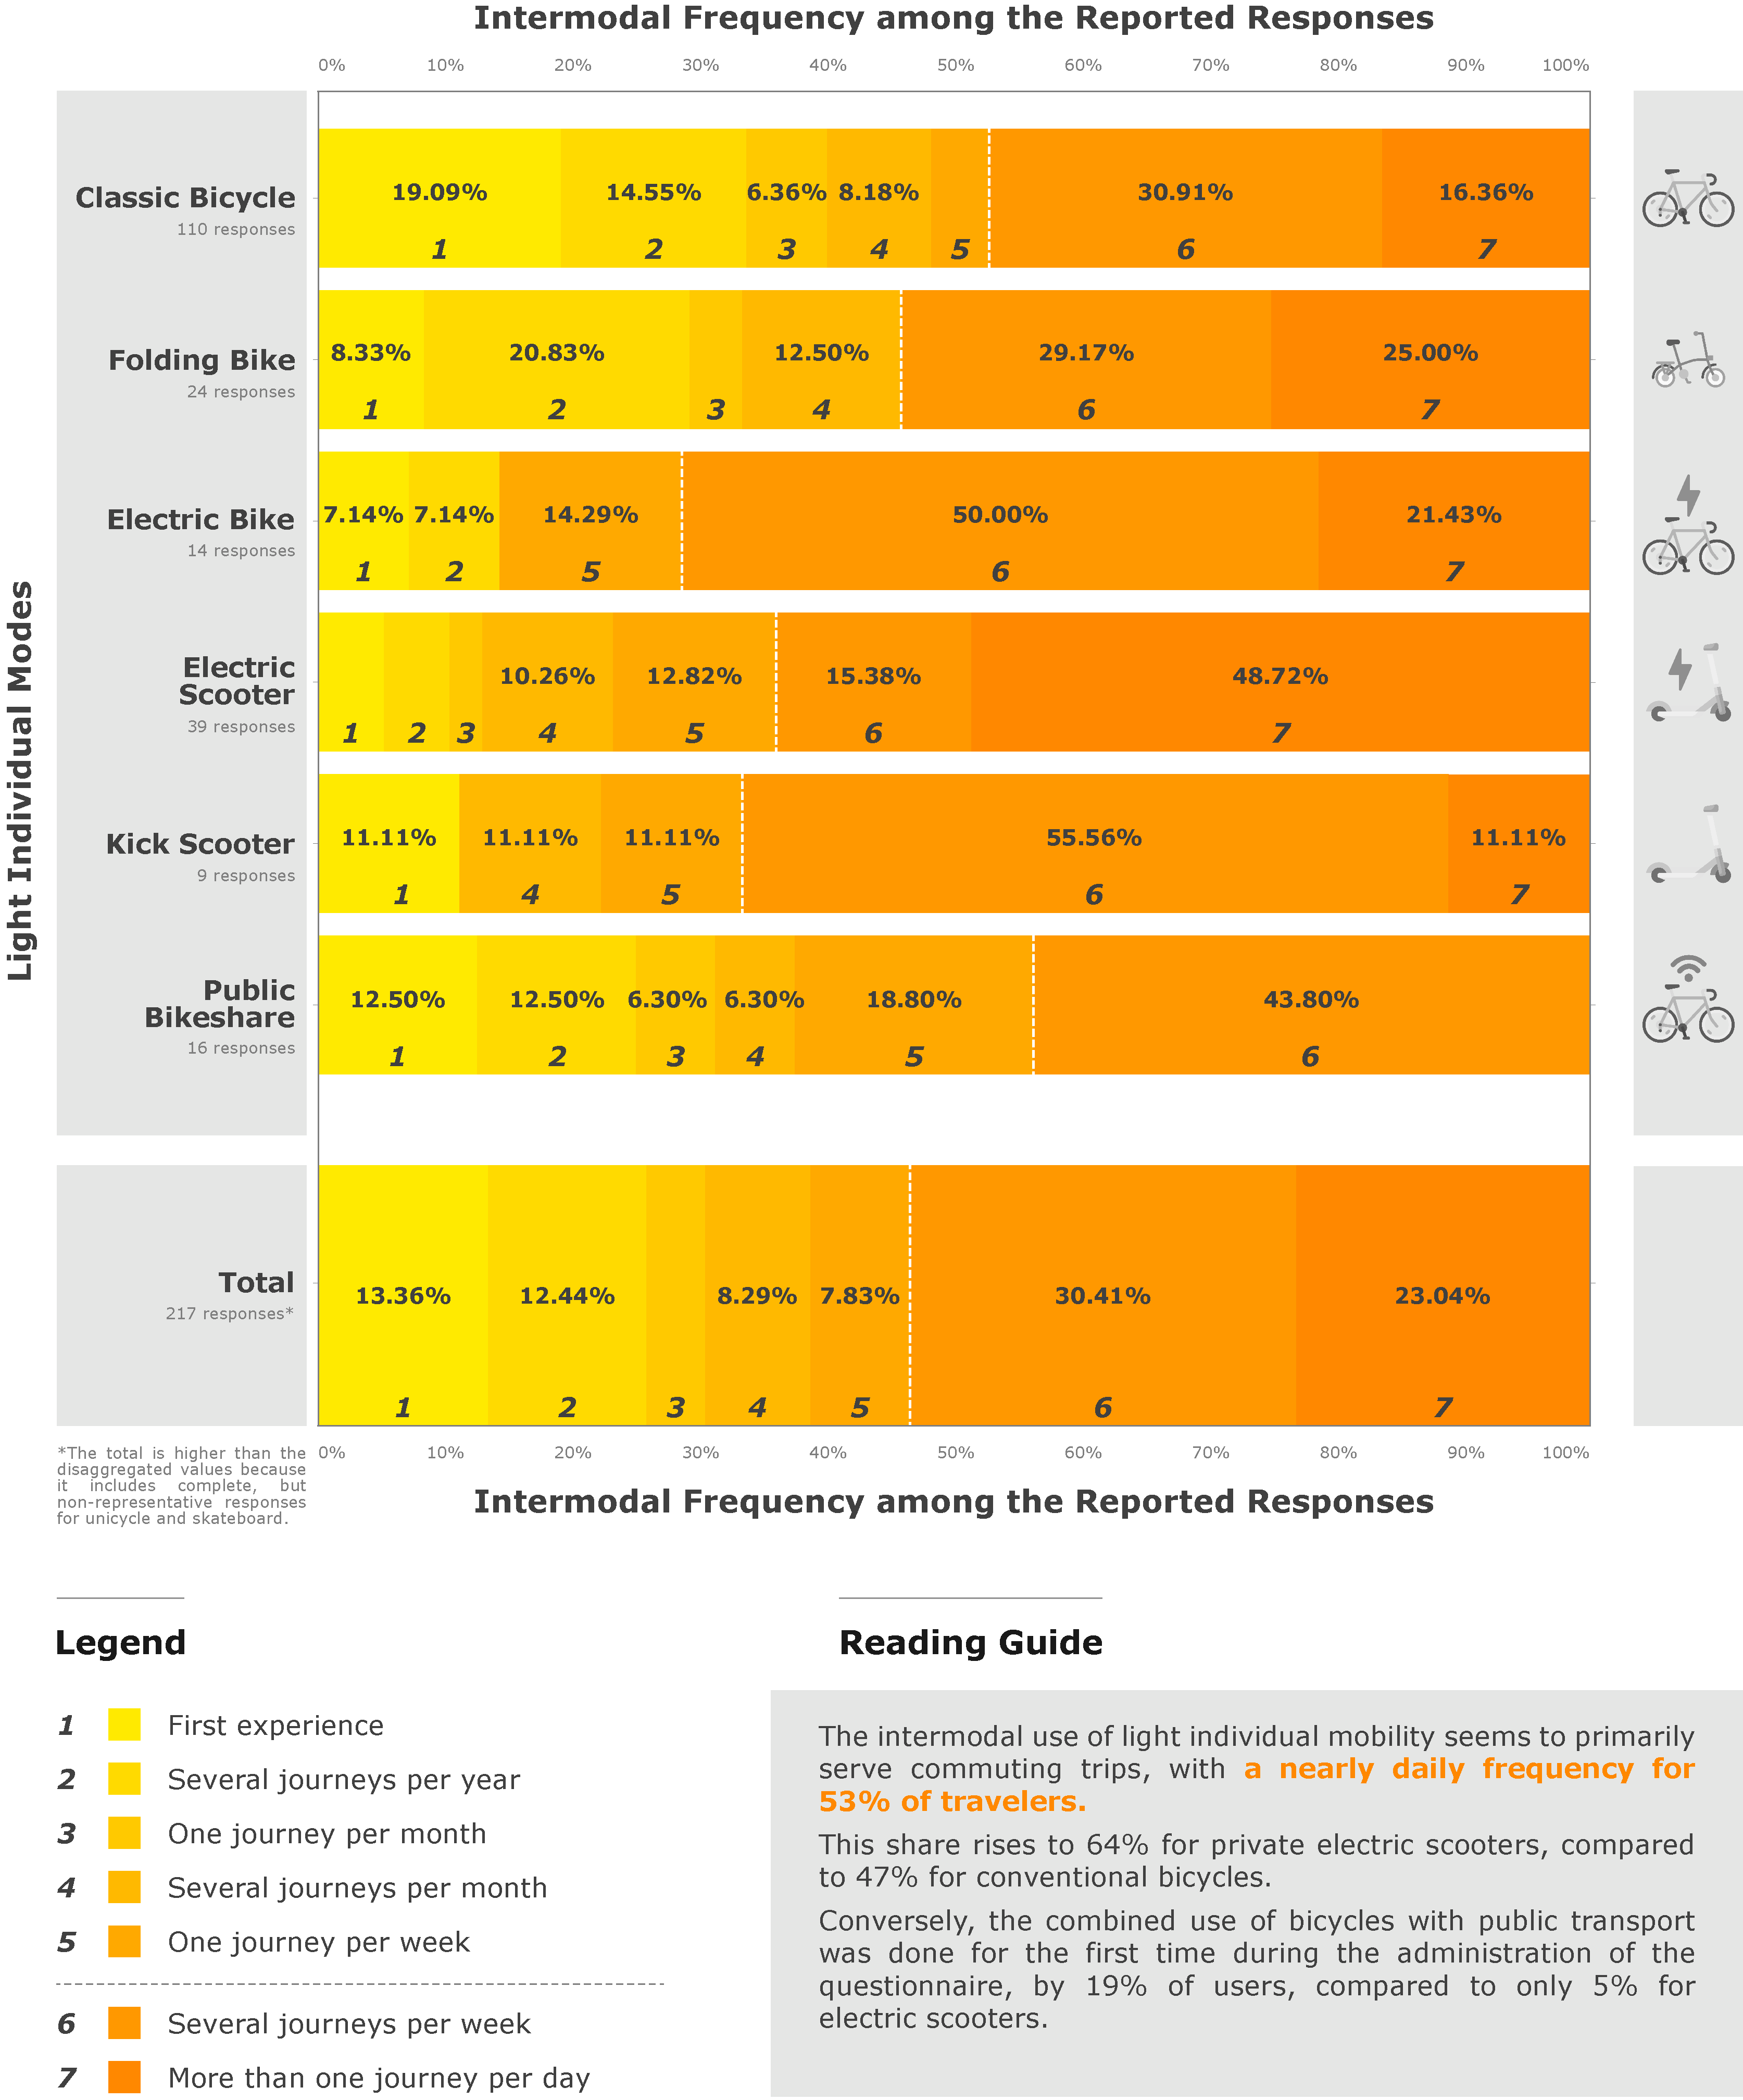
\includegraphics[width=1\columnwidth]{src/Figures/Chap-4/EN_Frequence.pdf}}
    \vspace{5pt}
    \begin{flushright}\scriptsize{
    Author: \textcolor{blue}{Dylan Moinse (2023)}
    }\end{flushright}
\end{figure}

% Fréquence - modes
The integration of light individual mobility into the public transport system is characterized by almost daily use for the majority of the transport modes studied (see \hyperref[fig-chap4:frequence-modes]{Figure~\ref{fig-chap4:frequence-modes}}, page~\pageref{fig-chap4:frequence-modes}), except for the \acrshort{PBS}, \acrshort{DBS}, and \acrshort{DESS}, for which the share is 44\% (7 responses), as well as for conventional bicycles, at 47\% (52 responses). \textsl{On the other hand}, the \acrshort{PeS} records a near-daily use frequency of 64\% (25 responses), mechanical scooters at 67\% (6 responses), and \acrshort{e-Bike} at 71\% (10 responses).%%Translated%%

% Motifs - général
This statistical observation regarding the intermodal use frequency of light individual mobility is complemented by an analysis of travel motives (see \hyperref[fig-chap4:motifs-modes]{Figure~\ref{fig-chap4:motifs-modes}}, page~\pageref{fig-chap4:motifs-modes}). This additional level of information provides key insights into the frequency of use of various modal combinations by users. In this regard, the results reveal that the vast majority of participants in the survey are regular commuters, engaged in daily mobility. Among 100 intermodal travelers, 76 primarily use it to get to their place of work or study (165 responses). Next are leisure activities and shopping, mentioned by 19 participants (41 responses), as well as walking or tourism, cited by 5 of them (11 responses).%%Translated%%

% Figure fréquence modes
\begin{figure}[h!]\vspace*{4pt}
    \caption{Distribution of the Primary Declared Travel Motives.}
    \label{fig-chap4:motifs-modes}
    \centerline{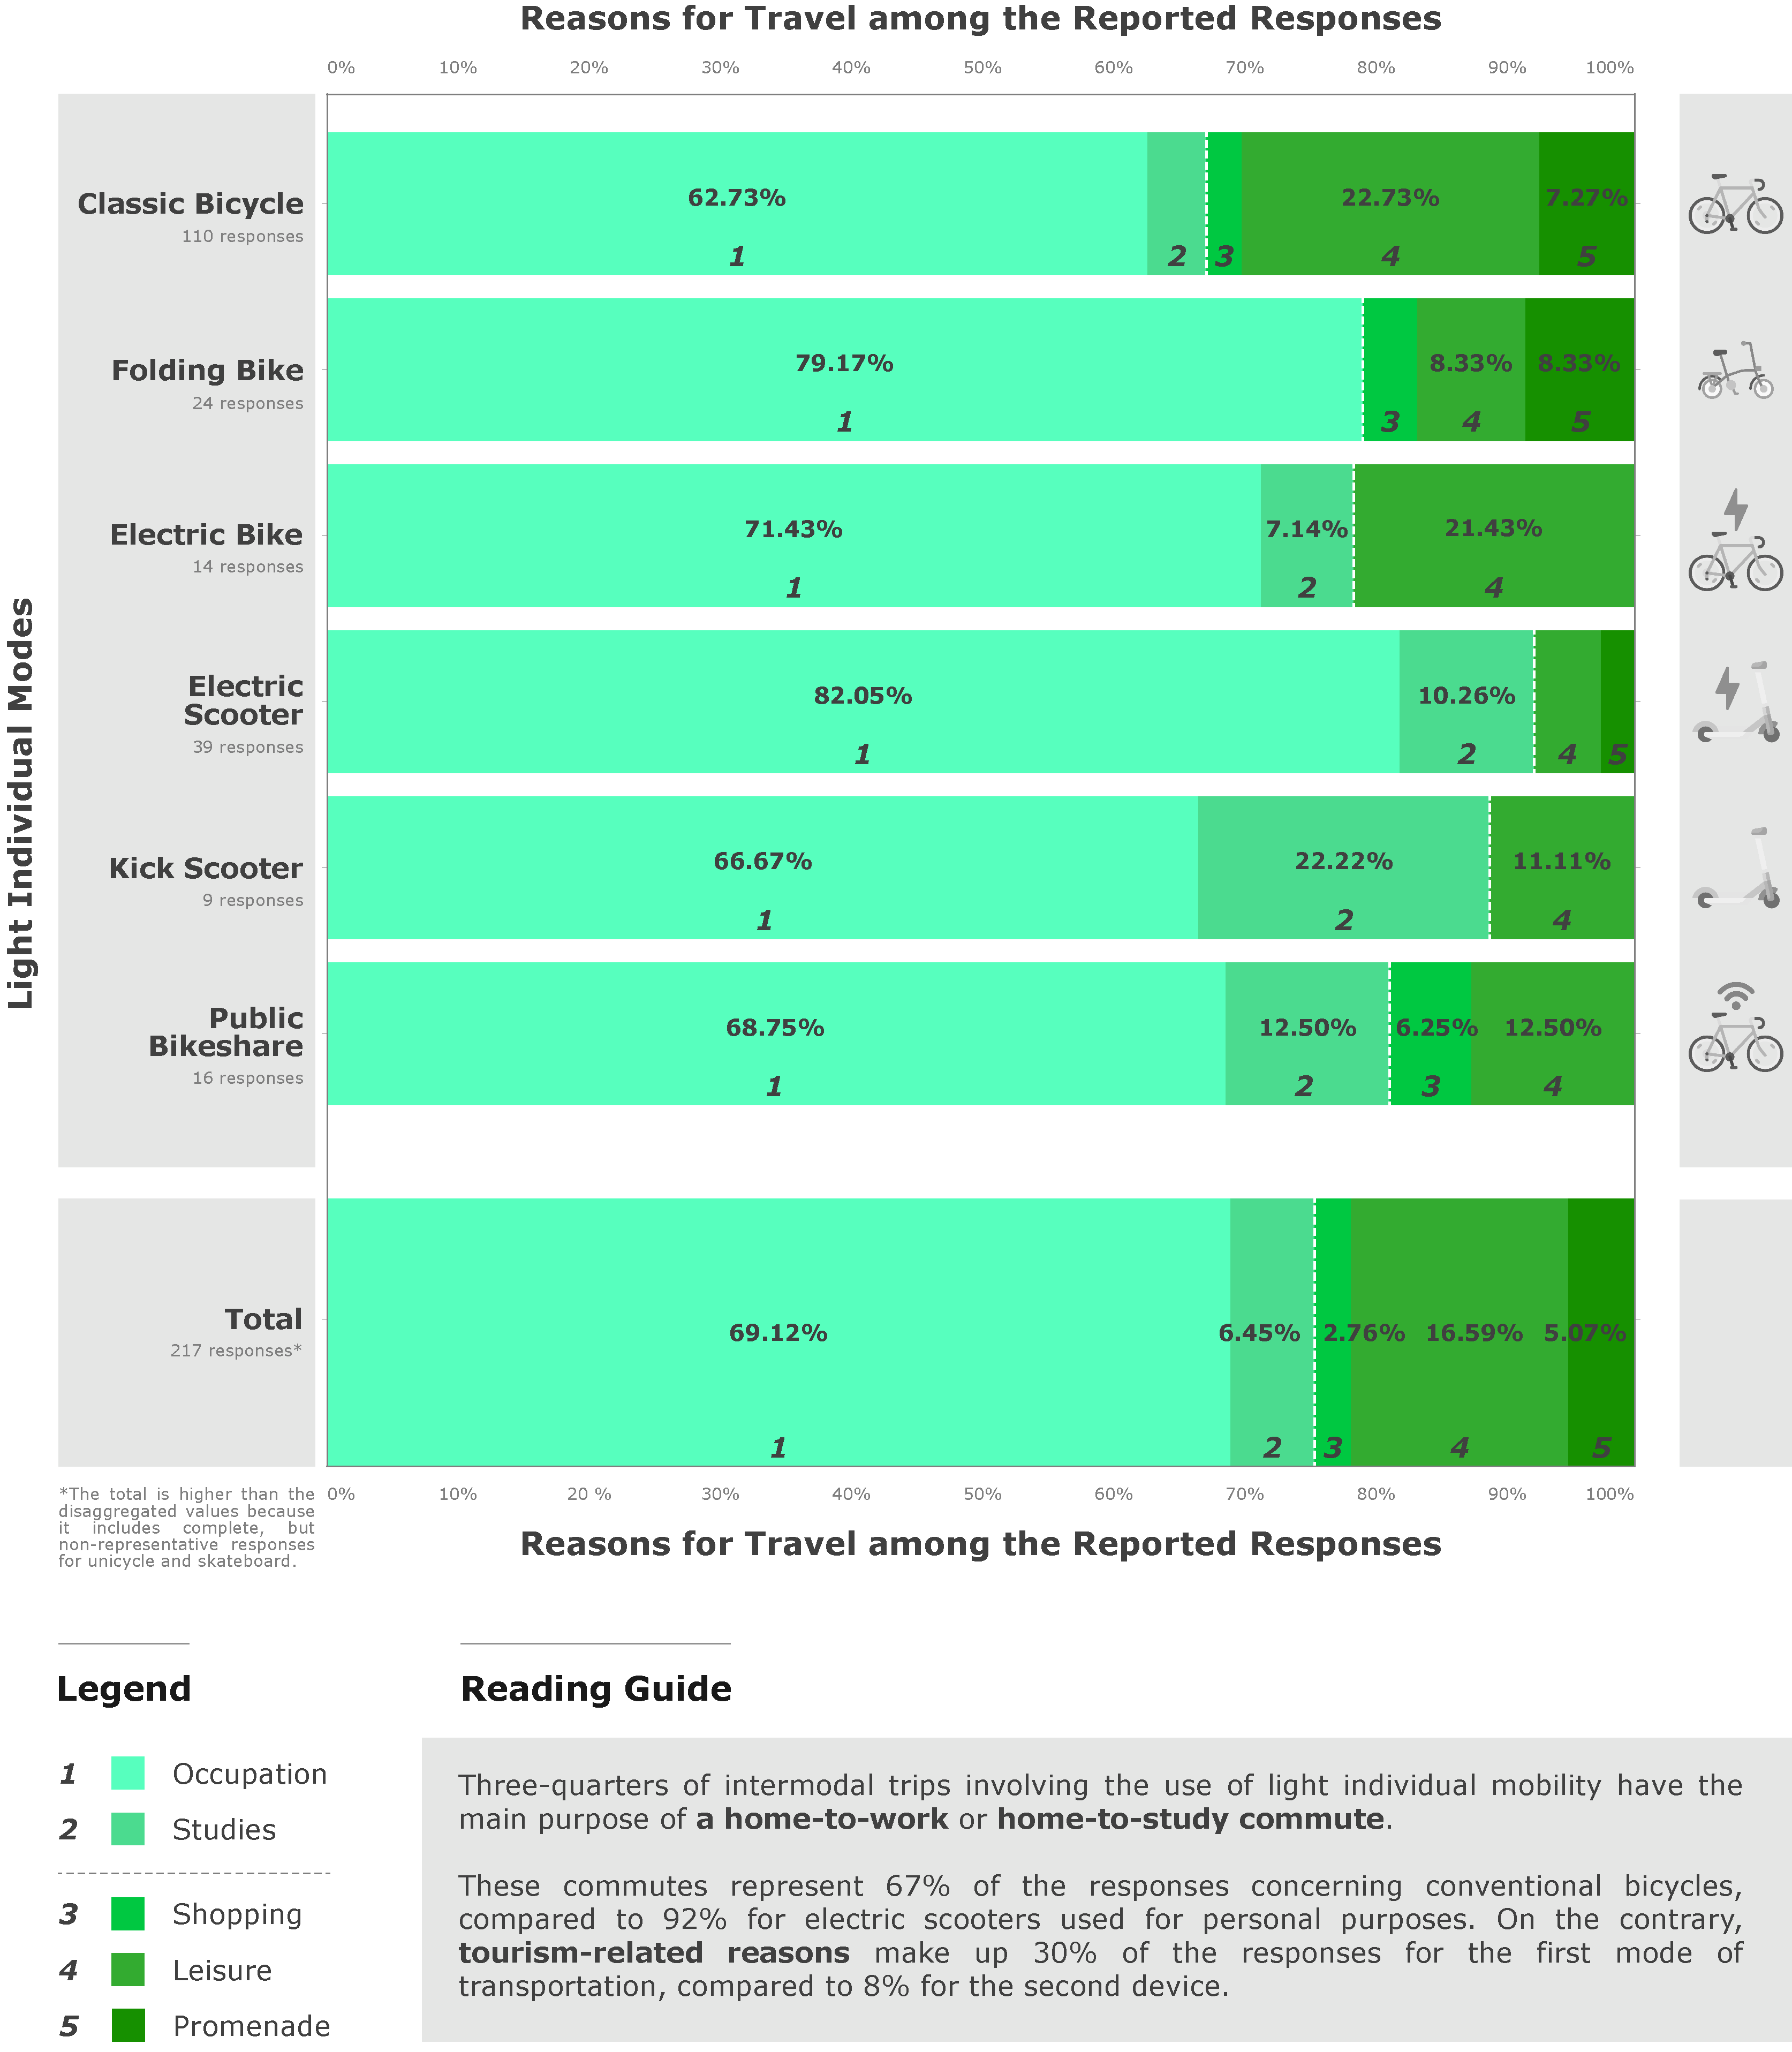
\includegraphics[width=1\columnwidth]{src/Figures/Chap-4/EN_Motifs.pdf}}
    \vspace{5pt}
    \begin{flushright}\scriptsize{
    Author: \textcolor{blue}{Dylan Moinse (2023)}
    }\end{flushright}
\end{figure}

% Fréquence + motifs - général
To better understand the interactions between usage frequency and travel motives, we made sure to cross these two variables. This analysis shows that 69\% of commuters are daily users. In contrast, among travelers whose trips are motivated by leisure or shopping, 52\% rarely engage in these intermodal practices, while 31\% of them made their trip in this way for the first time. This differentiation highlights a clear trend regarding the regularity of use based on the purpose of the trip.%%Translated%%

% Motifs - modes
A clear distinction is evident in the distribution of travel motives according to the type of vehicle chosen. Urban \Commas{glide} vehicles are proportionally more frequently used for commuting purposes than bicycles, particularly conventional bicycles, whose use is more diversified (see \hyperref[fig-chap4:motifs-modes]{Figure~\ref{fig-chap4:motifs-modes}}, page~\pageref{fig-chap4:motifs-modes}). Thus, 67\% of conventional bicycle users engage in these intermodal practices for commuting trips, while this share rises to 79\% for \acrshort{e-Bike}, 79\% for folding bicycles, 81\% for both \acrshort{PBS}, \acrshort{DBS}, and \acrshort{DESS}, 89\% for mechanical scooters, and 92\% for \acrshort{PeS}. This variation can be explained by the relatively higher use of bicycles by intermodal cyclists to complete their tourist trips. However, we observe that the daily frequency of use of these modal combinations does not exactly match the distribution of declared travel motives or the profiles of the users, who are almost all full-time workers. Even taking into account that teleworking can reduce the daily intermodal use of light individual mobility among individuals who can benefit from it, it seems that some of these users tend to alternate between the intermodal practices studied and other modes of transport during the same week.%%Translated%%

% Motifs par kilomètres parcourus
An additional step in the statistical analysis of the survey examines the distribution of intermodal trips according to different motives and their relative proportion in terms of spatial and temporal distances. Travel motives related to shopping, administrative tasks, social visits, and walks, although they represent a less significant share of intermodal uses associated with light individual mobility, stand out for having more extensive spatial and temporal distances compared to professional or educational activities. While intermodal trips for work account for 69\% of the declared motives, these commutes represent only 55\% of the miles traveled (\textsl{Vehicle Miles Traveled}, VMT) and 54\% of the total travel time. This gap is even more pronounced for home-to-school trips, which, representing 6\% of the responses, account for only 4\% of spatial distances and 4\% of time distances. In contrast, leisure activities, which make up 17\% of the survey responses, account for 38\% of the miles and 38\% of the declared time. These data support the importance of considering not only the purpose of trips associated with various activities but also their frequency, in relation to the spatial and temporal budgets allocated.%%Translated%%

% Littérature fréquence et motifs
Intermodal trips, combining the use of light individual mobility and trains, are predominantly characterized by their commuting nature. Our empirical observation aligns with current knowledge on trips combining public transport, bicycles, and micromobility. Scientific literature indicates that, generally, these commuters use these combined modes of transport more than four to five times a week \textcolor{blue}{\autocite[104]{flamm_public_2014}}\index{Flamm, Bradley~J.|pagebf}\index{Rivasplata, Charles~R.|pagebf} for professional or educational purposes, including both the use of personal bicycles \textcolor{blue}{\autocites[288]{martens_bicycle_2004}[16]{la_paix_puello_train_2016}[78]{oostendorp_combining_2018}[15]{shelat_analysing_2018}[8]{jonkeren_bicycle_2021}[184]{moinse_intermodal_2022}}\index{Shelat, Sanmay|pagebf}\index{Huisman, Raymond|pagebf}\index{Oort, Niels van|pagebf}\index{La Paix Puello, Lissy|pagebf}\index{Geurs, Karst~T.|pagebf}\index{Jonkeren, Olaf|pagebf}\index{Kager, Roland|pagebf}\index{Oostendorp, Rebekka|pagebf}\index{Gebhardt, Laura|pagebf}\index{Martens, Karel|pagebf}\index{Moinse, Dylan|pagebf}\index{Goudeau, Matthieu|pagebf}\index{L'Hostis, Alain|pagebf}\index{Leysens, Thomas|pagebf}, as well as \acrshort{PeS} \textcolor{blue}{\autocites[184]{moinse_intermodal_2022}[62]{rabaud_quand_2022}}\index{Moinse, Dylan|pagebf}\index{Goudeau, Matthieu|pagebf}\index{L'Hostis, Alain|pagebf}\index{Leysens, Thomas|pagebf}\index{Rabaud, Mathieu|pagebf}\index{Richer, Cyprien|pagebf}, and shared mobility services \textcolor{blue}{\autocites[68]{ma_understanding_2018}[10]{gu_measuring_2019}[18]{lin_analysis_2019}[394]{bocker_bike_2020}[10]{fan_dockless_2020}[11]{wang_spatiotemporal_2020}[10-11]{heumann_spatiotemporal_2021}[8]{kim_analysis_2021}[8]{qiu_interplay_2021}[8]{yu_understanding_2021}[8]{yu_policy_2021}}\index{Böcker, Lars|pagebf}\index{Anderson, Ellinor|pagebf}\index{Uteng, Tanu Priya|pagebf}\index{Throndsen, Torstein|pagebf}\index{Ma, Xinwei|pagebf}\index{Ji, Yanjie|pagebf}\index{Yang, Mingyuan|pagebf}\index{Jin, Yuchuan|pagebf}\index{Tan, Xu|pagebf}\index{Gu, Tianqi|pagebf}\index{Yu, Qing|pagebf}\index{Li, Weifeng|pagebf}\index{Yang, Dongyuan|pagebf}\index{Xie, Yingkun|pagebf}\index{Kim, Minjun|pagebf}\index{Cho, Gi-Hyoung|pagebf}\index{Yu, Senbin|pagebf}\index{Liu, Gehui|pagebf}\index{Yin, Congru|pagebf}\index{Lin, Diao|pagebf}\index{Zhang, Yongping|pagebf}\index{Zhu, Ruoxin|pagebf}\index{Meng, Liqiu|pagebf}\index{Qiu, Waishan|pagebf}\index{Chang, Hector|pagebf}\index{Heumann, Maximilian|pagebf}\index{Kraschewski, Tobias|pagebf}\index{Brauner, Tim|pagebf}\index{Tilch, Lukas|pagebf}\index{Breitner, Michael|pagebf}.%%Translated%%

% Transition
Having analyzed intermodal practices and identified the main trends related to the frequency and motives of travel, it is now necessary to focus on the underlying factors that drive these modal choices. The following section sheds light on the hierarchy of reasons motivating the adoption of these modal combinations.%%Translated%%

% 4.2.1.2.
\needspace{1\baselineskip} % Réserve de l'espace
\subsubsection*{Hierarchy of Reasons for Modal Adoption: \textsl{Reach}, \textsl{Flexibility}, and \textsl{Ecology}
    \label{chap4:raisons-adoption}
    }

% Raisons adoption - général
When asked about the main factors that motivated their choice to adopt these intermodal practices, participants ranked various dimensions. These aspects include certain comparative advantages of these modal chains, such as the spatio-temporal optimization of the \gls{itinerary}, the reduction of economic and environmental costs, the improvement of well-being, and the individual relationship to travel. The results of this survey highlight three predominant motives (see \hyperref[fig-chap4:classement-global-raisons]{Figure~\ref{fig-chap4:classement-global-raisons}}, page~\pageref{fig-chap4:classement-global-raisons}). At the forefront, \Commas{environmental sensitivity} is the most frequently cited reason (\(F\), 137 responses). It is followed by \Commas{excessive walking distance} (\(E\), 128 responses) and the search for \Commas{flexibility} (\(G\), 108 responses). Secondary reasons, but regularly selected, include the desire to \Commas{get some fresh air} (\(M\), 87 responses) and \Commas{freedom of movement} (\(H\), 83 responses). Finally, a third category of reasons emerges from the rankings, associated with \Commas{economic costs of car use} (\(C\), 56 responses), the \Commas{fun} aspect (\(I\), 50 responses), as well as the \Commas{door-to-door} properties of these modal combinations (\(L\), 49 responses), the gain in \Commas{comfort} (\(B\), 46 responses), and the presence of \Commas{cycling infrastructure} along the route (\(N\), 43 responses).%%Translated%%

% Raisons adoption - modes
However, disparities emerge at the detailed level of the different modes of transport that make up light individual mobility, such that the use of conventional bicycles primarily reflects environmental concerns, while the adoption of scooters is mainly driven by practical and economic considerations. Indeed, the primary motivation for modal adoption, related to \Commas{environmental sensitivity} (\(F\)), ranks first notably due to the responses from conventional bicycle users who predominantly rank it in first place (18\%), compared to second place for folding bicycles (13\%) and fourth for \acrshort{PeS} (11\%). In contrast, \Commas{excessive walking distance} (\(E\)) is the highest-rated criterion regardless of the type of vehicle (between 13\% and 18\%). As for the argument related to \Commas{flexibility} (\(G\)), it is relatively less valued by conventional bicycle users (10\%), compared to folding bicycles and \acrshort{PeS} (12\% and 15\%). More specifically, the adoption of conventional bicycles in intermodality is also marked by a stronger expression of the need for \Commas{freedom of movement} (\(H\), 11\%) and \Commas{getting fresh air} (\(M\), 10\%). Furthermore, \acrshort{PeS} stands out for its heightened sensitivity to the \Commas{economic costs of car use} (\(C\), 12\%). Among all the indicators studied, folding bicycles occupy an intermediate position between the mechanical vehicle and the electric vehicle.%%Translated%%

% Figure classement raisons adoption modale
\begin{figure}[h!]\vspace*{4pt}
    \caption{Ranking of the Reasons for the Intermodal Adoption of Light Individual Mobility.}
    \label{fig-chap4:classement-global-raisons}
    \centerline{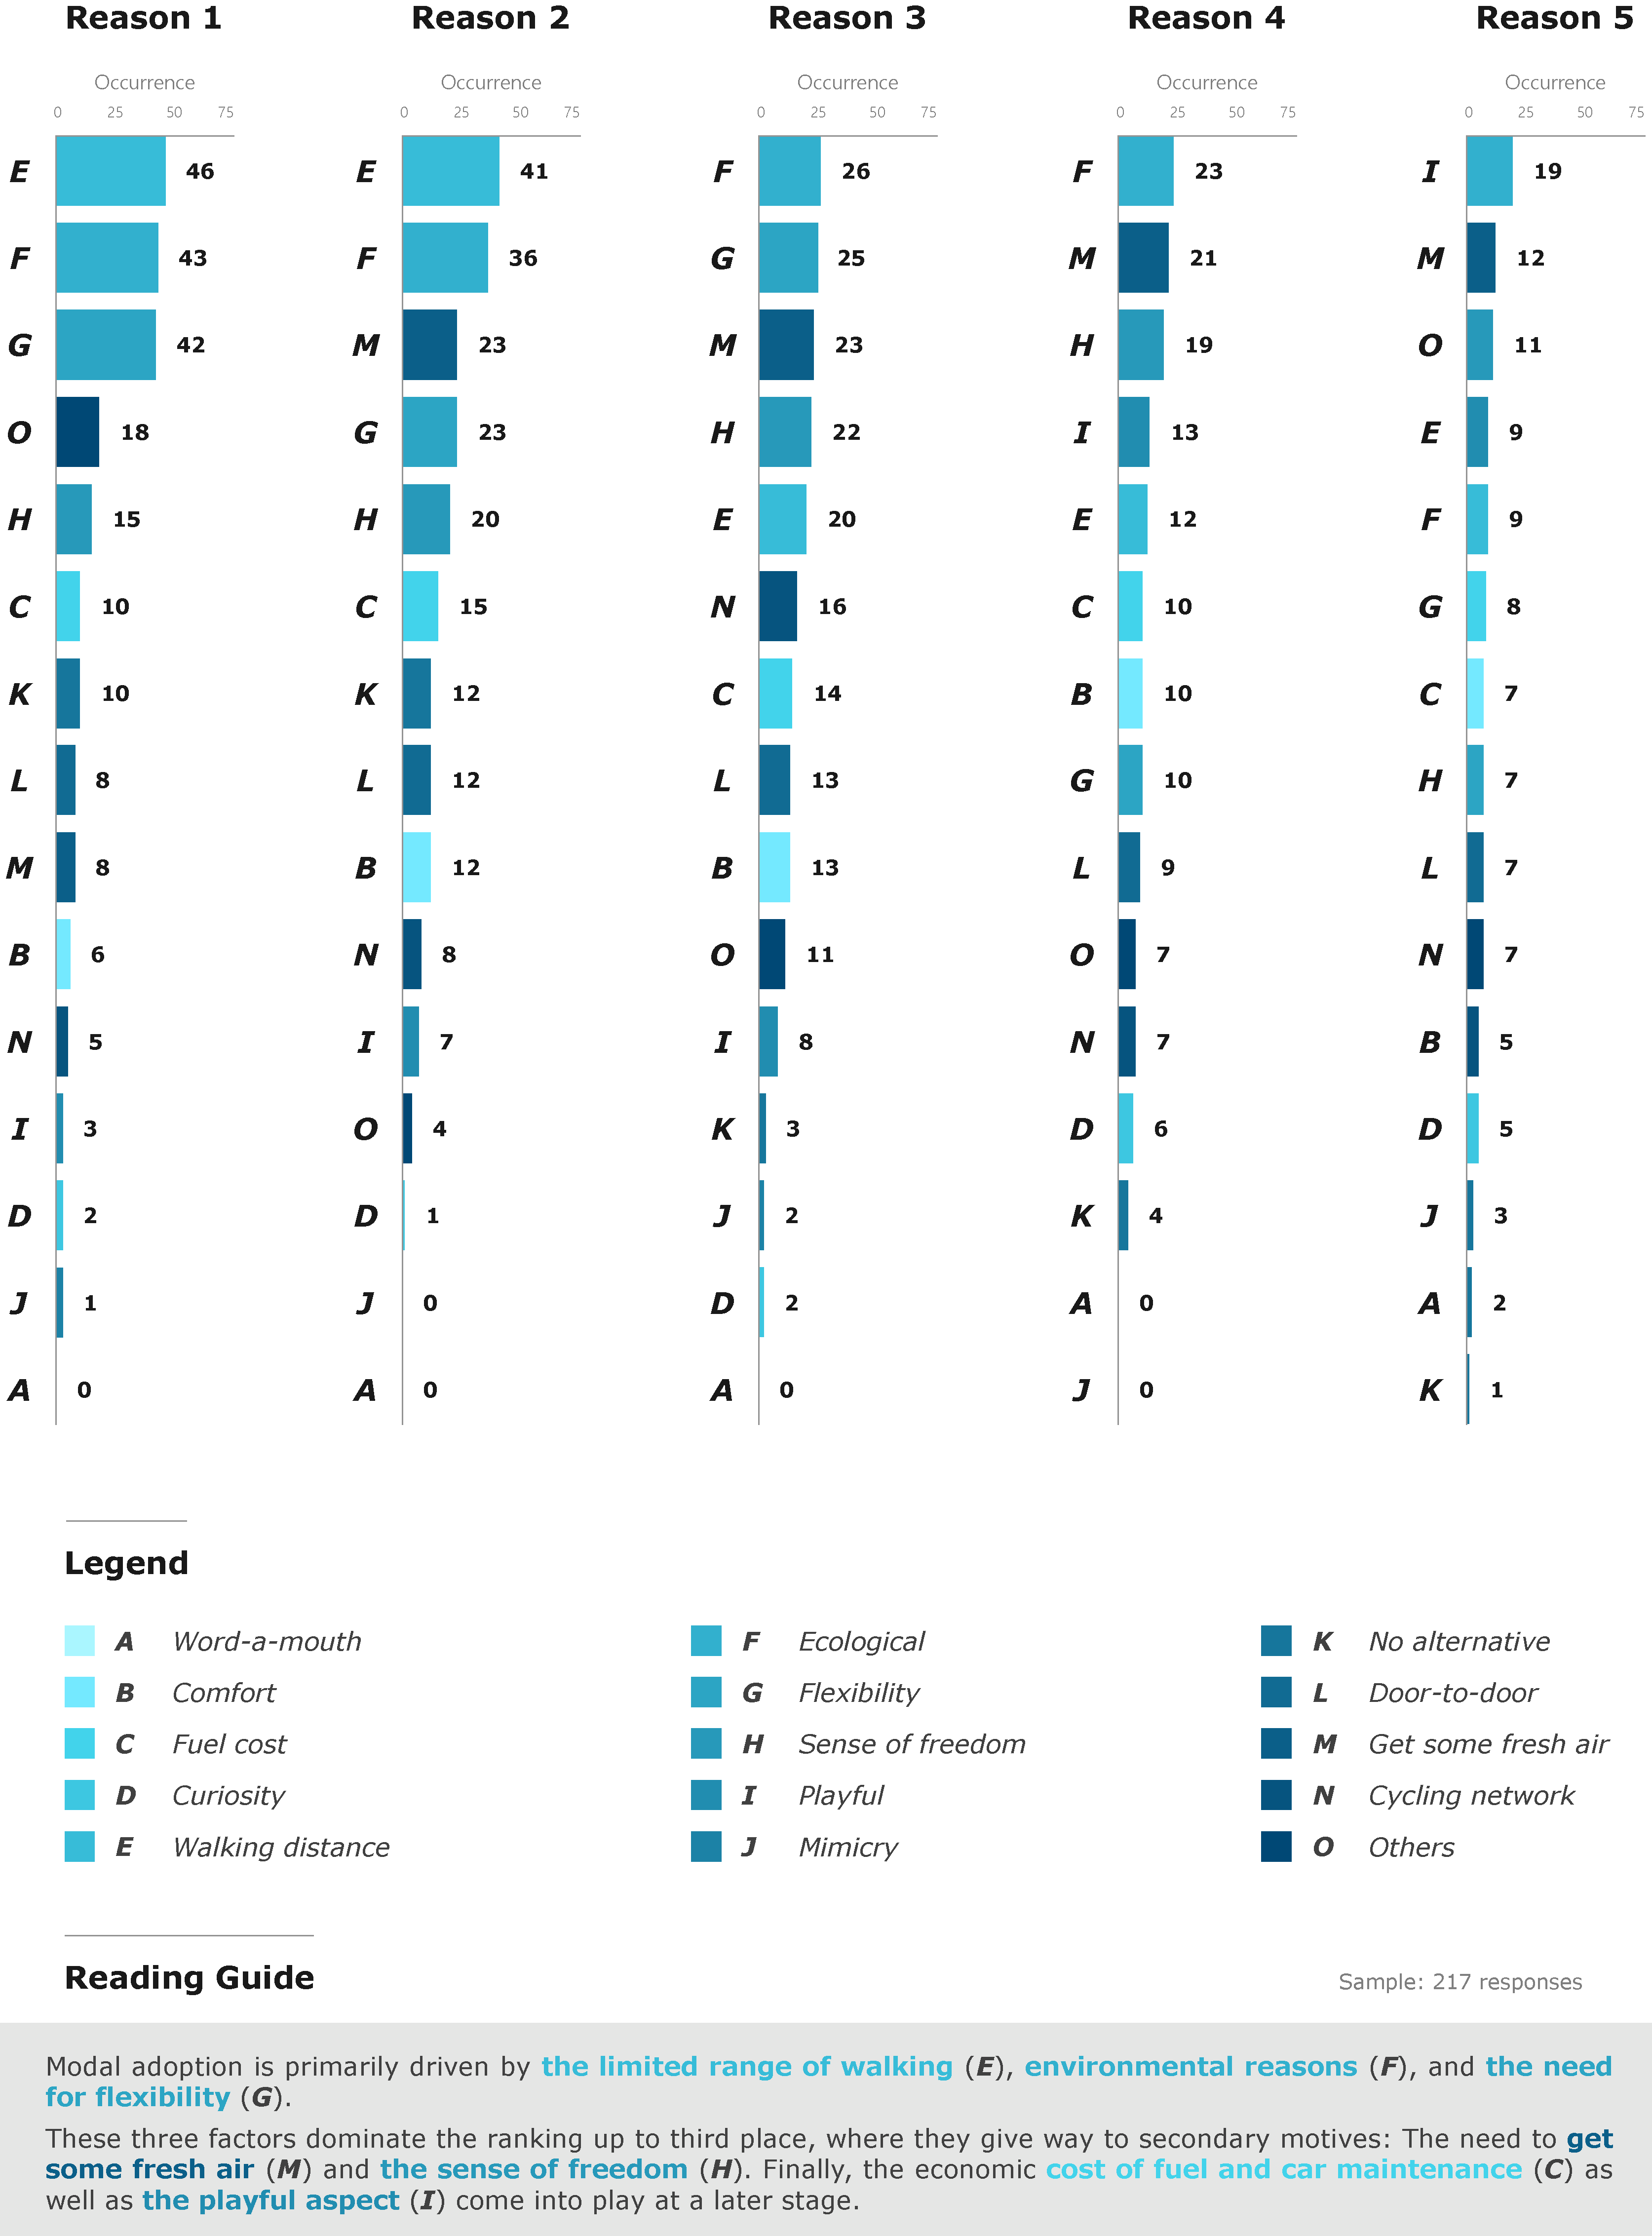
\includegraphics[width=1\columnwidth]{src/Figures/Chap-4/EN_Raisons_adoption.pdf}}
    \vspace{5pt}
    \begin{flushright}\scriptsize{
    Author: \textcolor{blue}{Dylan Moinse (2024)}
    }\end{flushright}
\end{figure}

% Approche raisons adoption - points
To consider the hierarchy of motives cited by participants to explain their modal choice, from the main reason to the fifth reason, we implemented a weighting system for the categorized criteria. This approach assigns points progressively based on the rank of each reason\footnote{~
    We used the Borda method (\textsl{Borda count method}) to assign points based on the preferences expressed by the voters, a system that has the advantage of not exclusively representing the top choices. The main reason grants five points to the ranked reason, with a decreasing system down to one point for the fifth reason. Variables that were not selected receive no points.
}. This technique, which goes beyond reasoning by occurrence, provides a differentiated distribution of modal choice motives (see \hyperref[table-chap4:raisons-adoption-modale-points]{Table~\ref{table-chap4:raisons-adoption-modale-points}}, page~\pageref{table-chap4:raisons-adoption-modale-points}).%%Translated%%

% Raisons adoption globale - points
Indeed, the three most frequently cited motivations—the \Commas{environmental sensitivity} (\(F\), 492 points), \Commas{excessive walking distance} (\(E\), 487 points), and \Commas{flexibility} (\(G\), 405 points) previously presented—retain their prominent positions. However, the \Commas{fun} (\(I\), 112 points) motivation has declined, while motivations associated with \Commas{freedom of movement} (\(H\), 266 points) and the desire to \Commas{get some fresh air} (\(M\), 255 points) remain steady. In contrast, some less frequently cited reasons are ranked higher, such as the \Commas{economic costs of car use} (\(C\), 179 points) and the \Commas{door-to-door} advantage (\(L\), 152 points).%%Translated%%

    % Tableau Raisons adoption par points
% Table Reasons for Adoption by Points
%%Rédigé%%
    \begin{table}[h!]
    \centering
    \renewcommand{\arraystretch}{1.5}
    \resizebox{\columnwidth}{!}{
    \begin{tabular}{p{0.07\columnwidth}p{0.06\columnwidth}p{0.4\columnwidth}p{0.1\columnwidth}p{0.1\columnwidth}p{0.1\columnwidth}}
        %\hline
    \rule{0pt}{15pt} \small{\textcolor{blue}{\textbf{Rank}}} & \small{\textcolor{blue}{\textbf{ID}}} & \small{\textcolor{blue}{\textbf{Ranked Reasons}}} & \small{\textcolor{blue}{\textbf{Points}}} & \small{\textcolor{blue}{\textbf{Top~3}}} & \small{\textcolor{blue}{\textbf{Sample Size}}}\\
        \hline
\small{1} & \small{\(F\)} & \small{Environmental awareness} & \small{\textbf{492}} & \small{105} & \small{137}\\
\small{2} & \small{\(E\)} & \small{Distances too long to walk} & \small{\textbf{487}} & \small{107} & \small{128}\\
\small{3} & \small{\(G\)} & \small{Flexibility gains} & \small{\textbf{405}} & \small{90} & \small{108}\\
        \hdashline
\small{4} & \small{\(H\)} & \small{Feeling of freedom} & \small{\textbf{266}} & \small{57} & \small{83}\\
\small{5} & \small{\(M\)} & \small{Getting fresh air} & \small{\textbf{255}} & \small{54} & \small{87}\\
\small{6} & \small{\(C\)} & \small{Economic costs of using a car} & \small{\textbf{179}} & \small{39} & \small{56}\\
\small{7} & \small{\(O\)} & \small{Other declared reasons} & \small{\textbf{164}} & \small{33} & \small{51}\\
\small{8} & \small{\(L\)} & \small{Door-to-door route} & \small{\textbf{152}} & \small{33} & \small{49}\\
\small{9} & \small{\(B\)} & \small{Comfort of the journey} & \small{\textbf{142}} & \small{31} & \small{46}\\
\small{10} & \small{\(N\)} & \small{Presence of a bike lane network} & \small{\textbf{126}} & \small{29} & \small{43}\\
\small{11} & \small{\(K\)} & \small{Lack of alternatives} & \small{\textbf{116}} & \small{25} & \small{30}\\
\small{12} & \small{\(I\)} & \small{Fun} & \small{\textbf{112}} & \small{18} & \small{50}\\
\small{13} & \small{\(D\)} & \small{Curiosity} & \small{\textbf{37}} & \small{5} & \small{16}\\
\small{14} & \small{\(J\)} & \small{Mimicry} & \small{\textbf{14}} & \small{3} & \small{6}\\
\small{15} & \small{\(A\)} & \small{Word-of-mouth} & \small{\textbf{2}} & \small{0} & \small{2}\\
    \hdashline
\multicolumn{3}{l}{\small{\textbf{General Average}}} & \small{\textbf{197}} & \small{\textbf{59}} & \small{\textbf{-}}\\
        \hline
        \end{tabular}}
    \caption{Distribution of points for reasons of intermodal adoption of light individual mobility.}
    \label{table-chap4:raisons-adoption-modale-points}
        \vspace{5pt}
        \begin{flushleft}\scriptsize{
        \textcolor{blue}{Note:} The \textsl{Points} column refers to the number of points assigned in a decreasing order to each reason, with the first position of the ranking receiving five points and the fifth position receiving one point. The \textsl{Top~3} column refers to the number of times the option was ranked in the top three choices among the responses provided.
        \\
        \textcolor{blue}{Reading Guide:} Based on the 217 responses analyzed, the results show that environmental awareness and the perception of distances being too long to walk are the two main reasons for adopting intermodal light individual mobility, followed by flexibility gains, which complete the top three reasons expressed.
        }\end{flushleft}
        \begin{flushright}\scriptsize{
        Author: \textcolor{blue}{Dylan Moinse (2024)}
        }\end{flushright}
        \end{table}%%Rédigé%%

% Raisons adoption par modes - points
In the same way, we chose to analyze in depth the similarities and disparities between the different modes of transport by employing this weighting system (see \hyperref[fig-chap4:raisons-adoption-modale-points-modes]{Figure~\ref{fig-chap4:raisons-adoption-modale-points-modes}}, page~\pageref{fig-chap4:raisons-adoption-modale-points-modes}). We observe a clear distinction between, on one hand, the intermodal adoption of human-powered modes, except for \acrshort{PBS}, primarily driven by ecological considerations and the freedom of movement, and, on the other hand, electric mobility users, who prioritize flexibility in relation to the financial burdens of car use. It appears that \Commas{environmental sensitivity} (\(F\)) accounts for 21\% of the total points for conventional bicycles and 23\% for mechanical scooters. This proportion decreases to 16\% for folding bicycles, 12\% for \acrshort{e-Bike}, and even to 10\% and 9\% respectively for mobility services and \acrshort{PeS}. Indeed, for electric and folding vehicles, \Commas{flexibility} (\(G\)) is more highly valued, representing 19\% of the points, as it is also for mechanical scooters and folding bicycles, which record 18\% and 17\%, respectively. \Commas{Economic costs of car use} (\(C\)) is another predominant criterion, rising to 13\% for \acrshort{PeS}. In contrast, the sense of \Commas{freedom of movement} (\(H\)) is much more emphasized by users who adopted bicycles of all types, compared to scooters of all types and shared mobility.%%Translated%%

% Figure treemap raisons adoption modale par modes et par points
\begin{figure}[h!]\vspace*{4pt}
    \caption{Treemap by Points of Reasons for Intermodal Adoption by Vehicle Type.}
    \label{fig-chap4:raisons-adoption-modale-points-modes}
    \centerline{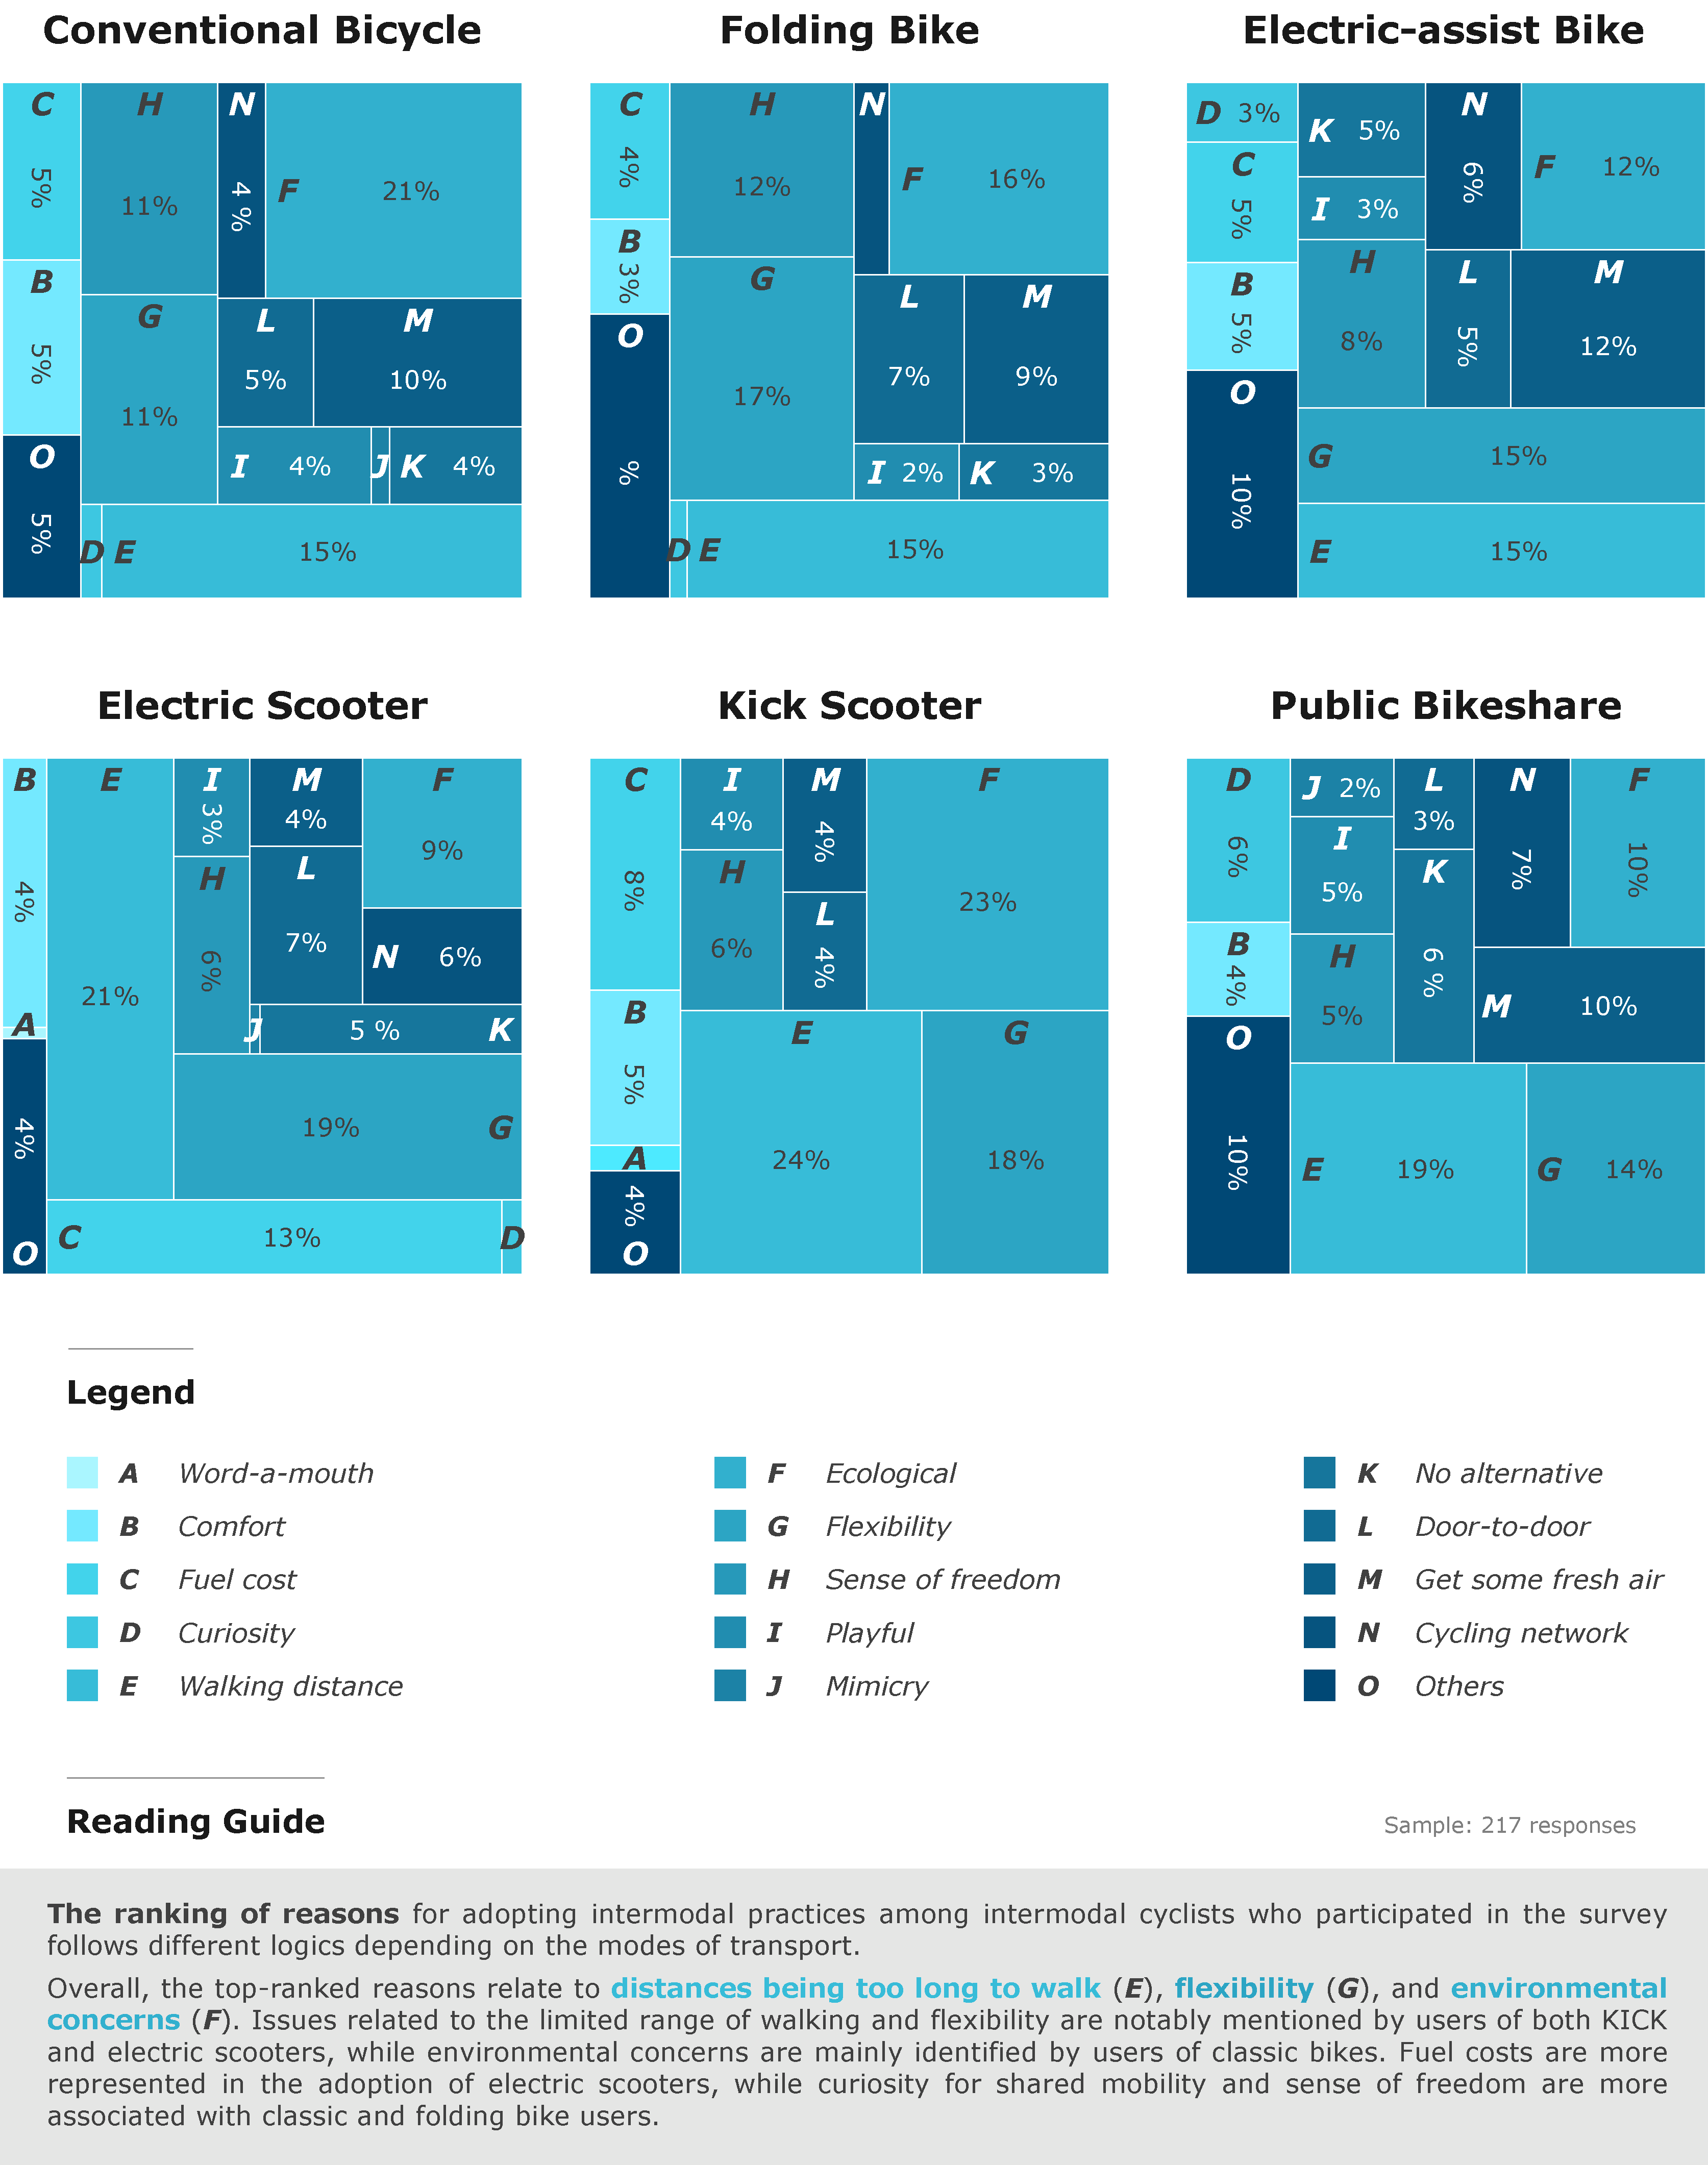
\includegraphics[width=1\columnwidth]{src/Figures/Chap-4/EN_Treemap_raisons_adoption.pdf}}
    \vspace{5pt}
    \begin{flushright}\scriptsize{
    Author: \textcolor{blue}{Dylan Moinse (2024)}
    }\end{flushright}
\end{figure}

% Raisons autres - global
A significant number of rankings, however, included responses of the \Commas{other} type, enriched with free-text answers. Among the 51 additional reasons mentioned and detailed by the respondents, the pursuit of \Commas{time-distance gains} (17 responses) emerges as the most frequently cited argument. This motivation is followed by the search for \Commas{benefits for physical condition} (9 responses), \Commas{cost savings on urban public transport subscriptions} (6 responses), and a solution to \Commas{automobile congestion parking problems} (6 responses). Other textual responses were grouped around \Commas{reducing waiting times at bus stops} (5 responses), \Commas{greater flexibility outside peak hours} (3 responses), a \Commas{substitute during strike periods} (3 responses), and in reaction to \Commas{incentive measures implemented by the employer} (2 responses).%%Translated%%

% Raisons autres - hiérarchie
In terms of the classification of motivations influencing modal choice, \Commas{time-distance gains} (72 points) remain predominant, frequently occupying the top position, along with \Commas{automobile congestion parking problems} (24 points). Some categorized reasons are considered secondary, such as \Commas{benefits for physical condition} (21 points), \Commas{reducing waiting times at bus stops} (17 points), and \Commas{greater flexibility outside peak hours} (10 points). In contrast, while \Commas{cost savings on urban public transport subscriptions} (9 points) are frequently mentioned, they are often relegated to the status of a minor motivation.%%Translated%%

% Littérature raisons adoption
Several studies have focused on the factors influencing the adoption of light individual mobility, when used exclusively. Our observations align with the general trends that identify the main motives for adopting these modes of transport: the search for time savings and a sense of freedom of movement, followed by environmental and economic motivations. \textcolor{blue}{\textcite[16-17]{pages_nouveaux_2021}}\index{Pages, Thibaud|pagebf}\index{Lammoglia, Adrien|pagebf}\index{Josselin, Didier|pagebf} looked into the attractive elements of \acrfull{NIEV} in France, primarily including monocycles, \acrshort{e-Bike}, and \acrshort{PeS}. Their results highlight, as the top choice, a desire to \Commas{change mode} (27\%), \Commas{save time} (18\%), \Commas{be outdoors} (17\%), \Commas{environmental reasons} (16\%), \Commas{save money} (13\%), and to enjoy greater \Commas{flexibility in route selection} (9\%). Furthermore, a similar classification from the study conducted by \textcolor{blue}{\textcite[15]{smart_mobility_lab_usages_2020}}\index{Smart Mobility Lab@\textsl{Smart Mobility Lab}|pagebf} indicates that users of a \acrfull{PMD} in a monomodal context particularly value \Commas{autonomy} and \Commas{reduced travel time}. These reasons are followed by \Commas{economic} and \Commas{fun} considerations, as well as \Commas{environmental} and \Commas{futuristic} aspects, while the emphasis on physical activity is marginal. Finally, a survey conducted among train travelers in France supports similar motivations behind their modal choice: practicality, speed, and the ecological and economic benefits of public transport services \textcolor{blue}{\autocite[24]{toluna_francais_2023}}\index{Toluna@\textsl{Toluna}|pagebf}\index{Harris Interactive@\textsl{Harris Interactive}|pagebf}.%%Translated%%

% Transition
This subsection supports the emerging nature of the integration of light individual mobility into the public transport network, particularly driven by the recent introduction of certain vehicles on the market. However, it remains uncertain whether this evolution represents a genuine advancement of the alternative mobility system, rather than a mere replacement of traditional modes of transport, typically bicycles, with the vehicles studied. In this context, we are led to investigate the modal substitution effect induced by the intermodal use of bicycles and micromobility.%%Translated%%

% 4.2.1.3.
\needspace{1\baselineskip} % Reserve space
\subsubsection*{A Double-Edged Modal Substitution Effect
    \label{chap4:substitution-modale-double-tranchant}
    }

% Modal Substitution - Global
To address the issue of the modal substitution effect of the interaction between light individual mobility and public transport, we included a specific question on modal competition in the survey for cycle commuters. We asked the following question: \Commas{If you had not been able to use your bicycle or personal transport device, what other mode would you have used to reach your departure station or destination from the arrival station?} (see \hyperref[annexes:structure-questionnaire-usagers]{Annex~\ref{annexes:structure-questionnaire-usagers}}, page~\pageref{annexes:structure-questionnaire-usagers}). The analysis of the responses reveals that the majority of participants would be able to adapt by replacing their vehicle with other modes of transport. Specifically, in the case of unavailability of their bicycle or micromobility for access or egress, 78\% of respondents would opt for another mode of transport either for a feeder or distribution service (169 responses), while 13\% would consider completely altering their modal choice for the entire intermodal journey (29 responses). Finally, 9\% of respondents would forgo the trip altogether (19 responses). %%Translated%%

% Modal Substitution - Feeder and Distribution
The collected data illustrate the marked tendency of respondents to favor certain modes of transport in the absence of their first choice for transfers to and from public transport hubs. In particular, urban public transport systems and combined walking emerge as preferred alternatives, with notable variations between the stages of their reference intermodal journey. For both feeder and distribution, 43\% of participants would switch to urban public transport to access the origin station (72 responses), compared to 38\% when leaving the destination station (64 responses). Combined walking is preferred by 37\% of respondents for the feeder stage (63 responses), compared to 54\% for the distribution stage (91 responses). Only 8\% of travelers would turn to car use for access (13 responses), either as a driver or passenger, while this modal shift drops to 1\% and 6\% respectively for egress (12 responses). Shared mobility is chosen by 3\% of respondents, exclusively for the feeder stage (5 responses). Finally, the option of taxi and \acrfull{RHS} represents 2\% for the \Commas{first kilometers} and 1\% for the \Commas{last kilometers} of the reported responses (5 responses). %%Translated%%

% Total Substitution
Among those who completely forgo the collective mode during the projected journey (13\%, 29 responses), the collected data show a strong inclination among respondents to opt for private car use, unlike the previously mentioned transfer modes. 76\% of them would prefer to use the car exclusively as a driver (22 responses). Carpooling, representing 14\% of the choices (4 responses), and car use as a passenger, at 7\% (2 responses), remain marginal, as does the scooter, which attracts only 3\% of respondents (1 response). %%Translated%%

% Synthesis
In all the scenarios considered, modal shift primarily favors walking and urban public transport, with 42\% and 37\% (154 and 136 responses) of the expressed preferences, respectively. Car driving follows with 10\% (37 responses), while the role of passenger, also known as \textsl{kiss-and-ride}, is chosen by 7\% of participants (25 responses). Can we therefore infer that the intermodal use of light individual mobility primarily replaces combined walking? In this regard, statistical analysis indicates that the choice of walking is often associated, at the ends of the intermodal journey, with car use: travelers who reported walking from the station are frequently drivers using a feeder mode. This phenomenon reveals an underlying complexity in the configuration of intermodal journeys, where combined walking is the mode most vulnerable to modal substitution. However, at the same time, car use is also replaced by the intermodal practices studied. This duality suggests that, although walking may be frequently replaced, it remains closely linked, within the mobility behaviors specific to cycle commuters, to car use. %%Translated%%

% Figure Modal Substitution Distances - Walking
\begin{figure}[h!]\vspace*{4pt}
    \caption{Estimation of modal shift from combined walking based on the spatial distances covered in transfer, by bicycle, and micromobility.}
    \label{fig-chap4:distances-substitution-modale}
    \centerline{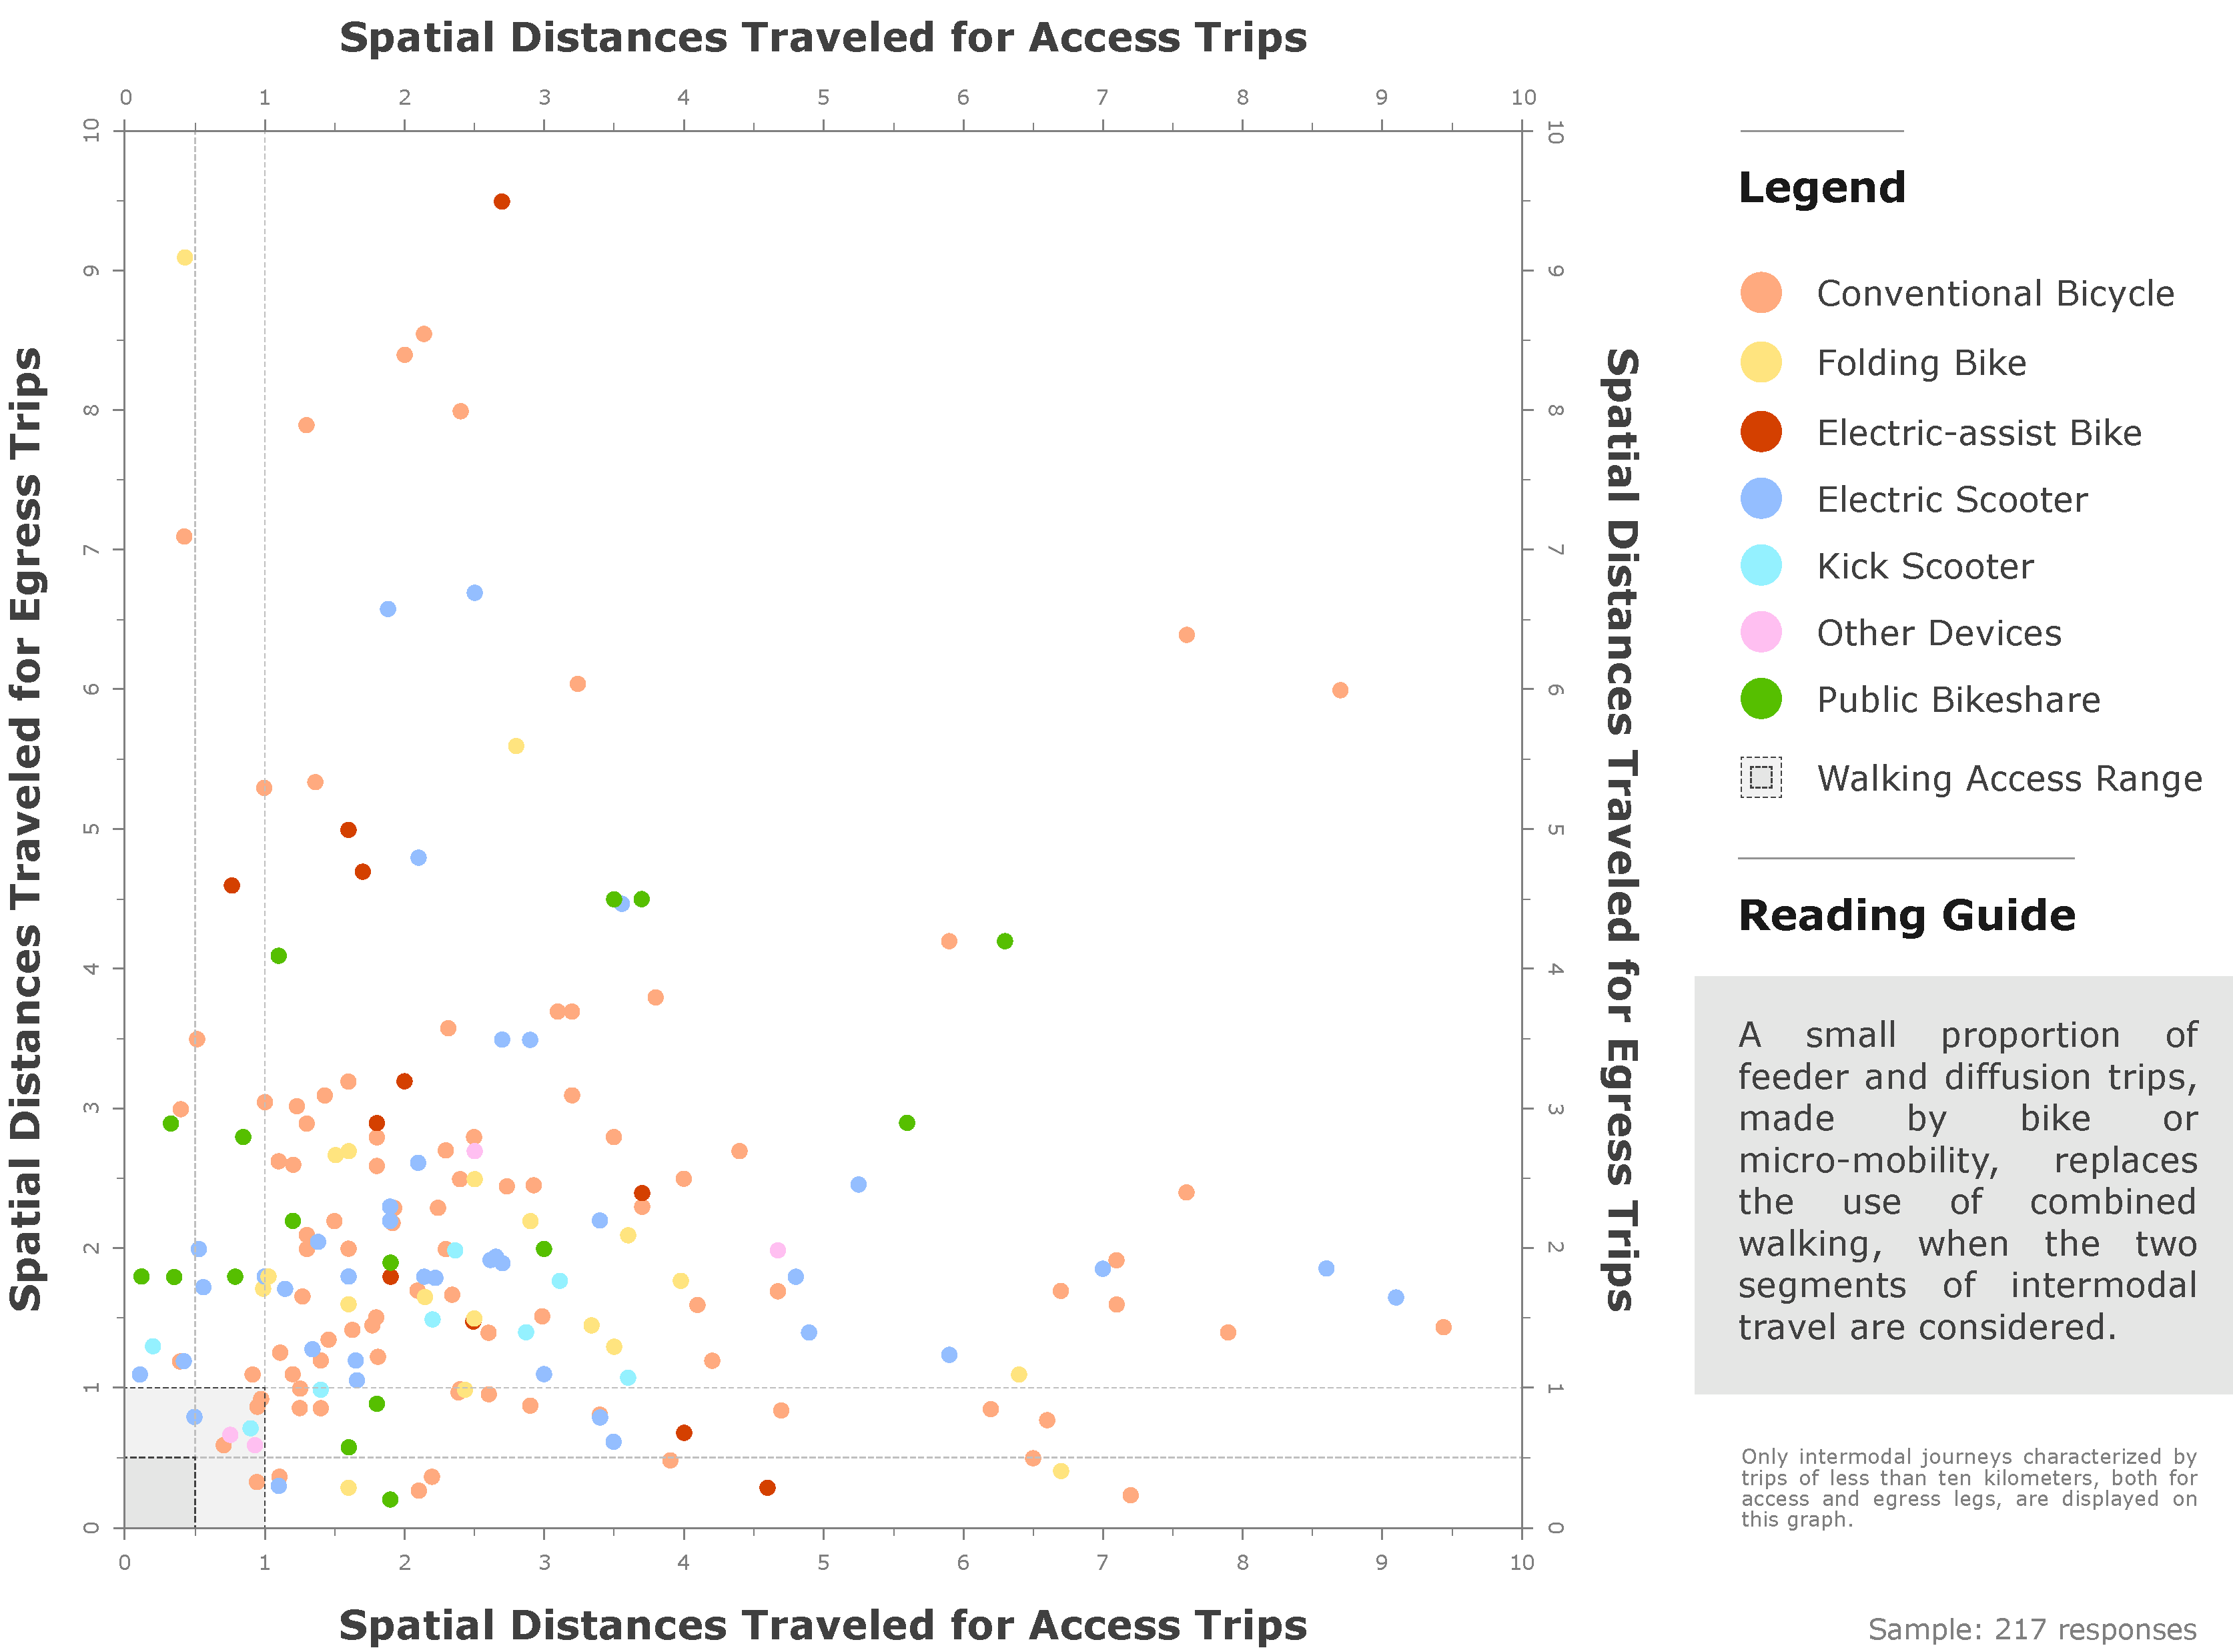
\includegraphics[width=1\columnwidth]{src/Figures/Chap-4/EN_Distances_substitution_modale.pdf}}
    \vspace{5pt}
    \begin{flushright}\scriptsize{
    Author: \textcolor{blue}{Dylan Moinse (2023)}
    }\end{flushright}
\end{figure}

% Distance reduction and diffusion
The argument that the substitution of combined walking reflects a double-edged impact on modal choices can be supported by a detailed analysis of the spatial distances covered by intermodal travelers. The aim is to go beyond the declared nature of responses to determine to what extent certain trips, both in access and egress, could have been made on foot given the distance traveled. Of the 358 trips made by bicycle or micromobility, only 12 routes are shorter than 0.50 kilometers and 38 remain under 1 kilometer. This represents 11\% of segments that could have been made on foot, assuming an extended scope for combined walking, of about 1 kilometer \textcolor{blue}{\autocite[34]{canepa_bursting_2007}}\index{Canepa, Brian|pagebf}. Among these 38 trips of less than 1 kilometer, 18 were made by regular bicycle, 8 by \acrshort{PeS}, 5 by folding bike, 4 by mechanical scooter, 2 by skateboard, and 1 by \acrshort{e-Bike}. Taking a relative perspective on the observed modal shares, the mechanical scooter and skateboard are the forms of micromobility that tend to replace combined walking the most.%%Translated%%

% Discussion on distance reduction and diffusion
However, a simultaneous analysis of the spatial distances covered in both access and egress segments shows that none of the trips display a distance of less than 0.50 kilometers for each segment of the intermodal journey. Furthermore, only 8 trips display distances of less than 1 kilometer on both sides of the trip (see \hyperref[fig-chap4:distances-substitution-modale]{Figure~\ref{fig-chap4:distances-substitution-modale}}, page~\pageref{fig-chap4:distances-substitution-modale}). This result suggests that only 2\% of trips made by bicycle or micromobility, as part of a modal chain, actually substitute combined walking. Responses based on a modal shift from walking then raise questions, as they indicate that, although walking was conceivable, it would not have been feasible over the entire \Commas{first and last mile}. In this respect, there seems to be a notable discrepancy between the walking modal substitution effect deduced from the route analysis and the one estimated by declared responses. This gap could then be explained by users' choice to opt for longer trips to or from public transport hubs that are not necessarily the closest to their departure or destination points, thanks to the use of light individual mobility, while pedestrian alternatives to closer stops might have been possible. This hypothesis will be further explored in the \hyperref[chap5:discussion-detours-pauses-optimisation]{section dedicated to the study of detours~\ref{chap5:discussion-detours-pauses-optimisation}} (page~\pageref{chap5:discussion-detours-pauses-optimisation}), in \hyperref[chap5:titre]{Chapter~5} (page~\pageref{chap5:titre}).%%Translated%%

% Real Modal Substitution
It is clear that the modal substitution effect in favor of light individual mobility coupled with public transport primarily comes at the expense of urban public transport networks, particularly bus services. This modal shift can be attributed to a certain distrust of the urban bus offer, which is seen as insufficiently competitive in the face of the growing demand for flexibility \textcolor{blue}{\autocite[19-24]{bauman_liquid_2000}}\index{Bauman, Zygmunt|pagebf}, which is better satisfied by light individual mobility. The participant in the commented journey, referred to as \(PCTE_{1}\), illustrates this situation by recounting her decision not to take the bus after arriving at Maubeuge station, due to the perceived excessive waiting time. She states that she would have traveled entirely by car if her \acrshort{PeS} had not been available, highlighting the loss of competitiveness of the train compared to the car in this context: \Commas{\textsl{The advantage too is being able to leave the station directly and arrive at the destination, without having to wait for the bus. I think the waiting time for the bus would have made me stop taking the train.} [\dots] \textsl{because I find myself having to take the bus in Maubeuge. And therefore having to buy a subscription, wait for the bus\dots~And in the evening, I'm not necessarily confident about waiting\dots}} [12:18 and 17:14, \(PCTE^{TC}_{1}\)]. Furthermore, this study also shows that intermodal practices can effectively replace the use of the car, enhancing the competitiveness of public transport when neither walking nor the bus provides a sufficiently agile alternative. The user \(PCTE_{2}\) explains that, although he is capable of walking to the République~-~Beaux-Arts metro stop, he prefers to travel by \acrshort{PeS} because his vehicle is essential for the egress segment, where walking would be too time-consuming. He then acknowledges that without his scooter, he would resort to using the car for the entire journey [08:20, \(PCTE^{TC}_{E}\)].%%Translated%%

% Mobility Change 1
Based on the analysis of the question regarding the mobility habits of the respondents in the questionnaire: \Commas{How often do you use these different modes of transportation?}, cross-referenced with the following question: \Commas{Do you use these different modes of transportation more or less frequently since you adopted these modal combinations?} (see \hyperref[annexes:structure-questionnaire-usagers]{Annex~\ref{annexes:structure-questionnaire-usagers}}, page~\pageref{annexes:structure-questionnaire-usagers}), we were able to determine the effects of these intermodal practices on competing mobility systems at the individual level. To this end, each traveler who regularly uses one of the concerned modes of transportation was automatically redirected to the next question, asking whether their frequency of use had changed, ranging from \Commas{much less frequent}, \Commas{less frequent}, \Commas{stable}, \Commas{more frequent} to \Commas{much more frequent}.%%Translated%%

% Mobility Change 2
The survey revealed a marked trend towards reducing the use of taxis, \acrshort{RHS}, and cars, both as drivers and passengers, since the adoption of intermodal strategies (see \hyperref[fig-chap4:impacts-adoption-autres-modes]{Figure~\ref{fig-chap4:impacts-adoption-autres-modes}}, page~\pageref{fig-chap4:impacts-adoption-autres-modes}). Passenger car transportation experienced a decline in the use of these services, with 88\% of the responses indicating so (50 out of 57 responses). More specifically, 75\% reported a significant reduction (43 out of 57 responses). At the same time, the car, whether as a driver or passenger, tends to be less favored. For drivers, 68\% decreased their frequency of use (102 out of 151 responses), with 38\% mentioning a substantial reduction (57 out of 151 responses). As for passengers, 51\% reported a decrease (76 out of 150 responses), with 28\% mentioning a pronounced reduction (42 out of 150 responses). Conversely, the exclusive use of light individual mobility increased for nearly half of the respondents (48\%, 96 out of 201 responses), including 27\% who now use it \Commas{much more frequently} (54 out of 201 responses). Urban public transport presents a more nuanced picture: although 28\% of users reduced their usage (56 out of 203 responses), almost an equivalent proportion increased it (29\%, 58 out of 203 responses). The frequency of walking remains largely unchanged for the majority of respondents (58\%, 118 out of 209 responses), while 30\% walk less frequently (63 out of 209 responses), with 22\% doing so moderately (45 out of 209 responses).%%Translated%%

% Figure Impacts on Mobility Systems
\begin{figure}[h!]\vspace*{4pt}
    \caption{Impacts of intermodal practices on users' mobility habits.}
    \label{fig-chap4:impacts-adoption-autres-modes}
    \centerline{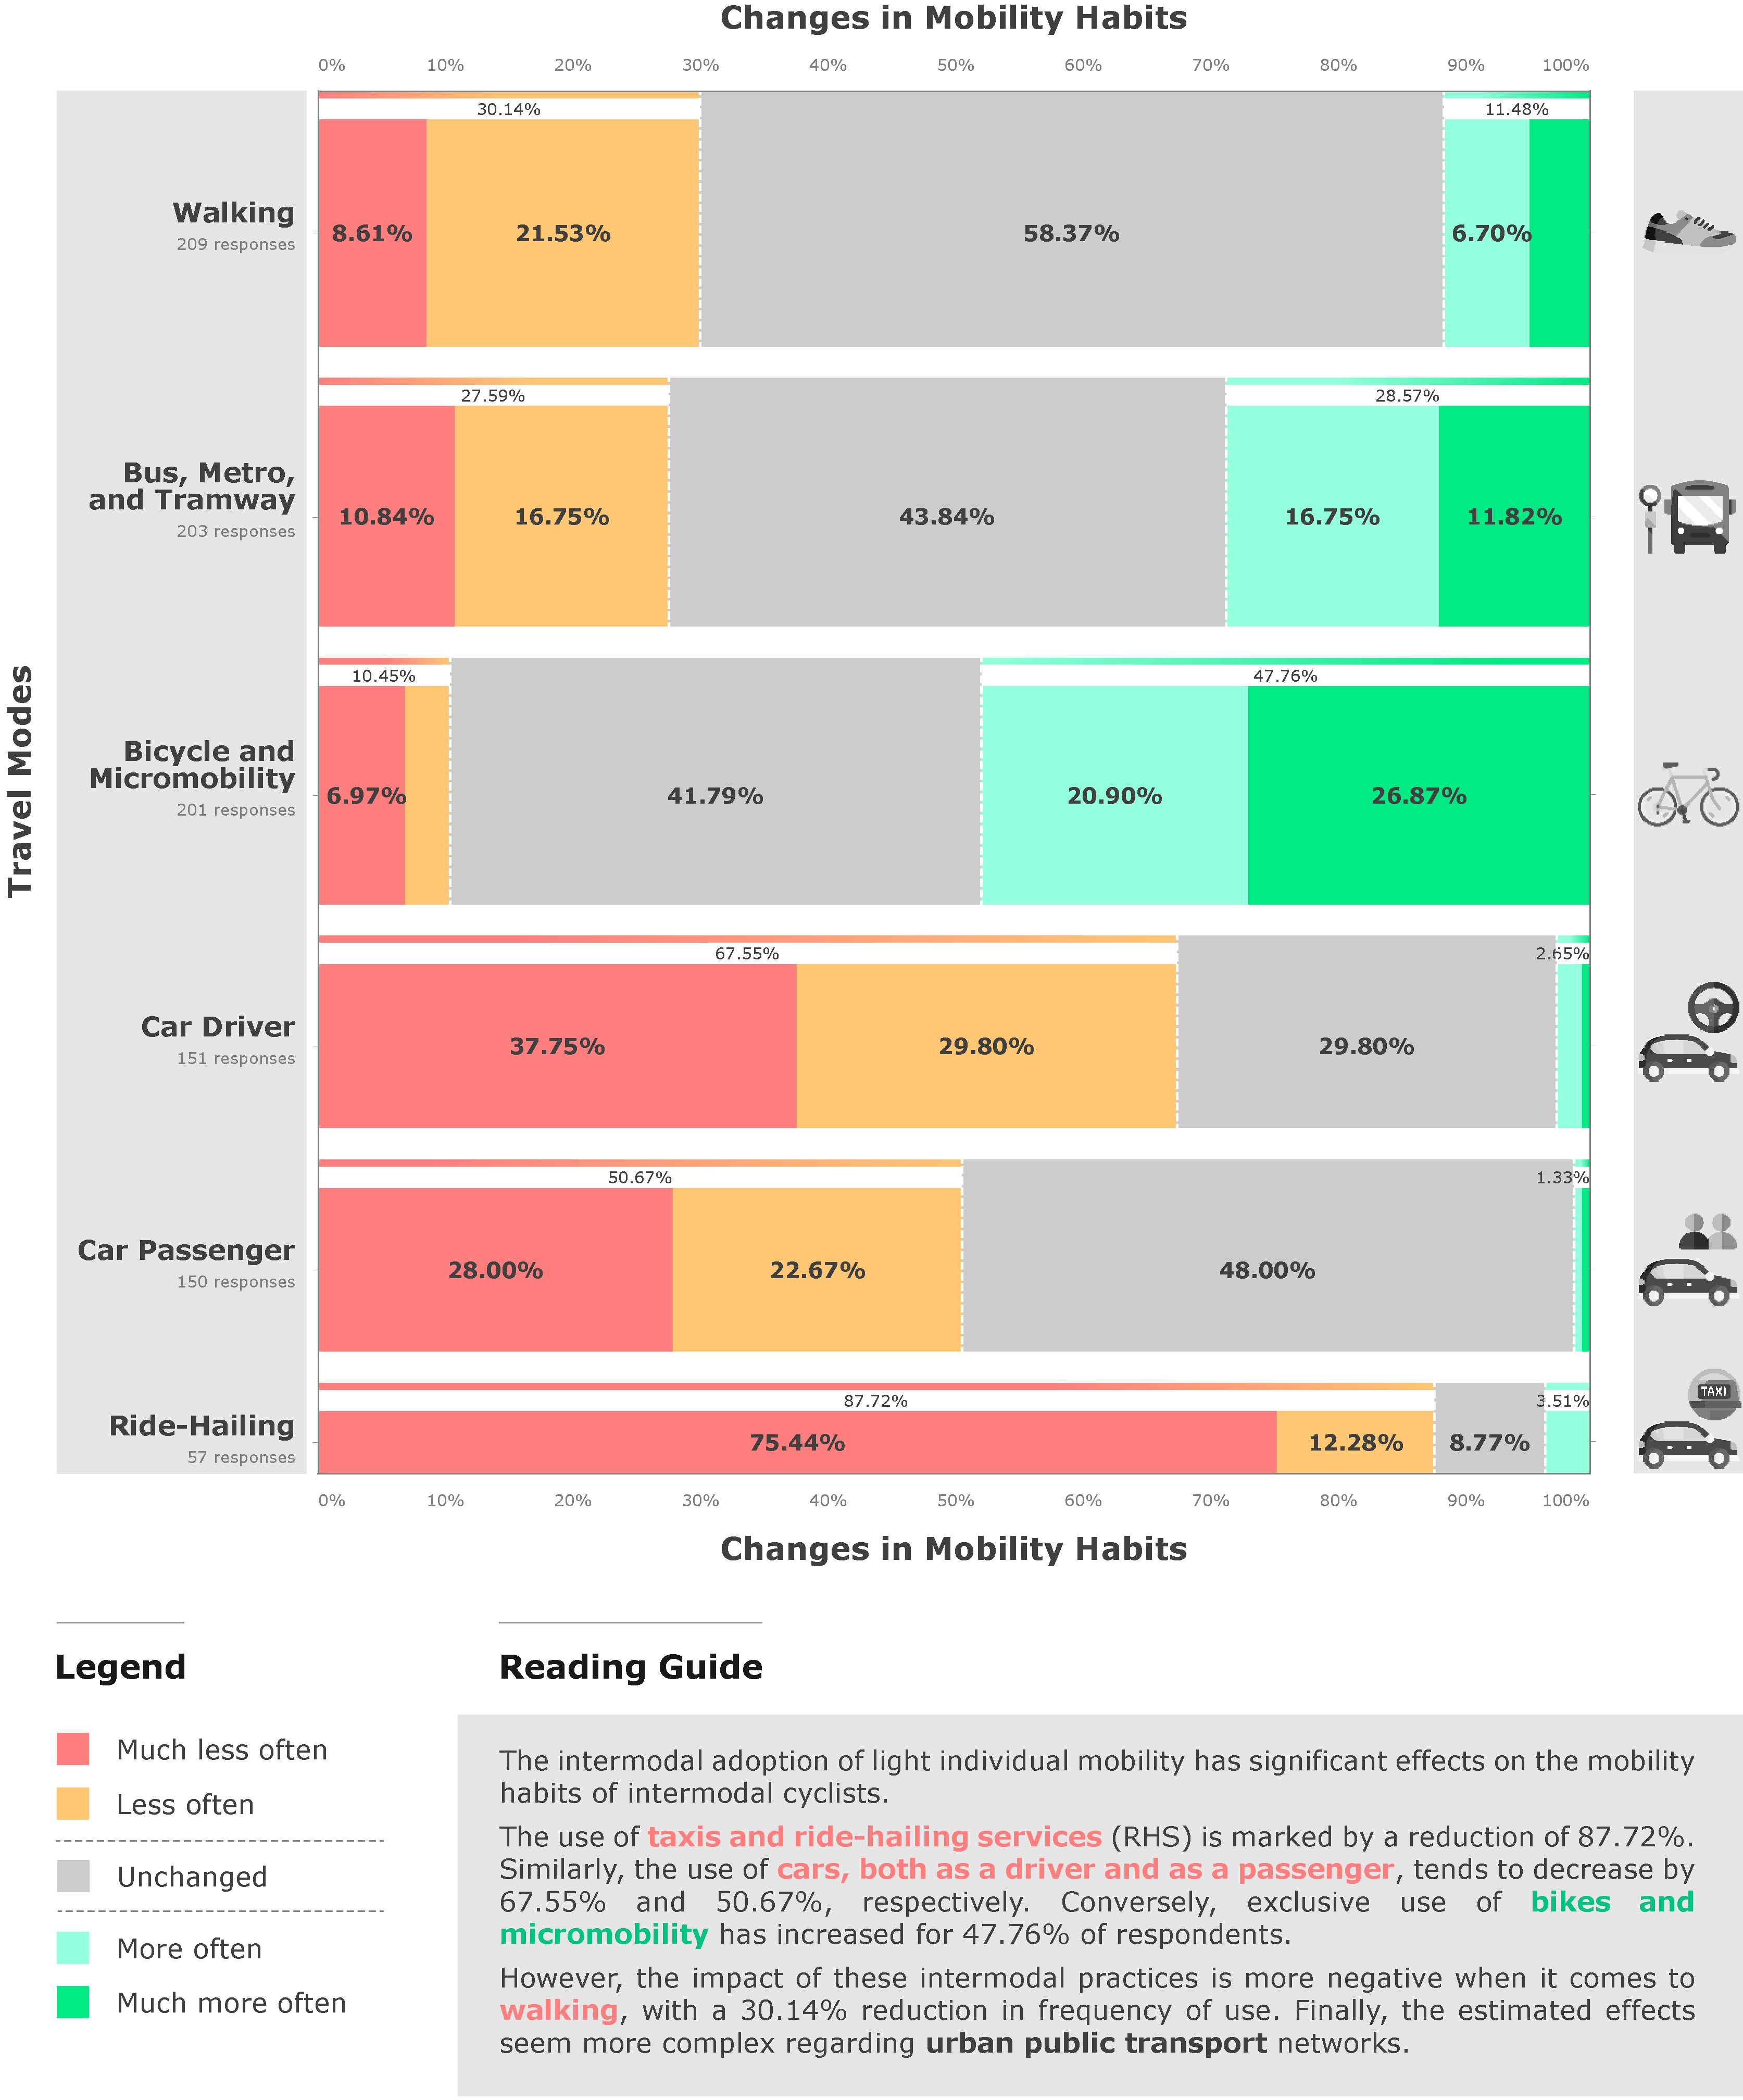
\includegraphics[width=1\columnwidth]{src/Figures/Chap-4/EN_Substitution_modale.pdf}}
    \vspace{5pt}
    \begin{flushright}\scriptsize{
    Author: \textcolor{blue}{Dylan Moinse (2023)}
    }\end{flushright}
\end{figure}

% Literature on Mobility Change - Car
Academic research partially supports the hypothesis that integrating light individual mobility into public transport systems contributes to a significant reduction in car use. In France, it was observed that 26\% of monomodal users of \acrshort{NIEV} switched from cars to these alternative modes of transport \textcolor{blue}{\autocite[14]{pages_nouveaux_2021}}\index{Pages, Thibaud|pagebf}\index{Lammoglia, Adrien|pagebf}\index{Josselin, Didier|pagebf}. These researchers also highlighted that the use of cars, as well as motorcycles and scooters, declined, reported by 70\% of \acrshort{NIEV} users \textcolor{blue}{\autocite[13]{pages_nouveaux_2021}}\index{Pages, Thibaud|pagebf}\index{Lammoglia, Adrien|pagebf}\index{Josselin, Didier|pagebf}. As for intermodal use of \acrshort{PBS}, the modal shift from cars to bikes in Montreal is estimated at 25\%, with a 40\% transition observed among residents of suburban areas \textcolor{blue}{\autocite[114]{bachand-marleau_much-anticipated_2011}}\index{Bachand-Marleau, Julie|pagebf}\index{Larsen, Jacob|pagebf}\index{El-Geneidy, Ahmed~M.|pagebf}. In Boston, \textcolor{blue}{\textcite[14]{basu_planning_2021}}\index{Basu, Rounaq|pagebf}\index{Ferreira, Joseph|pagebf} report a reduction in car ownership and solo driving, reflected by a 10\% decrease in miles traveled around transit stations three months after the introduction of a \acrshort{PBS} system. In New York City, intermodal use of the \acrshort{DESS} showed that the most significant substitution effects concerned carpooling, taxis, and \acrshort{RHS}, reaching 32\% \textcolor{blue}{\autocite[25]{lee_forecasting_2021}}\index{Lee, Mina|pagebf}\index{Chow, Joseph|pagebf}\index{Yoon, Gyugeun|pagebf}\index{He, Brian|pagebf}. However, some studies report that the impact of light individual mobility as a catalyst for modal shifts from cars remains limited in an intermodal context, as demonstrated by \textcolor{blue}{\textcite[12]{fan_how_2019}}\index{Fan, Aihua|pagebf}\index{Chen, Xumei|pagebf}\index{Wan, Tao|pagebf} in Beijing, with a modal shift rate of only 6\%, suggesting instead a reduction in walking and bus use.%%Translated%%

% Literature on Mobility Change - Walking and Bus
This section highlights a less favorable aspect of modal substitution attributable to light individual mobility, due to its negative impact on combined walking and particularly on bus networks. Indeed, in Taipei, intermodal travelers using \acrshort{PBS} prefer this service over walking, even for similar distances to public transport nodes \textcolor{blue}{\autocite[8]{yen_how_2023}}\index{Yen, Barbara~T.H.|pagebf}\index{Mulley, Corinne|pagebf}\index{Yeh, Chia-Jung|pagebf}. However, the bus remains the mode most directly challenged by the adoption of \acrshort{PBS}, \acrshort{DBS}, and \acrshort{DESS}, as observed in Tucson \textcolor{blue}{\autocite[16]{li_investigating_2022}}\index{Li, Xiaofeng|pagebf}\index{Wu, Yao-Jan|pagebf}\index{Khani, Alireza|pagebf}, Nanjing \textcolor{blue}{\autocite[12]{chen_what_2022}}\index{Chen, Wendong|pagebf}\index{Chen, Xuewu|pagebf}\index{Chen, Jingxu|pagebf}\index{Cheng, Long|pagebf}, Chengdu \textcolor{blue}{\autocite[107]{ma_impacts_2019}}\index{Ma, Xiaolei|pagebf}\index{Zhang, Xian|pagebf}\index{Li, Xin|pagebf}\index{Wang, Xingju|pagebf}\index{Zhao, Xu|pagebf} and Portland \textcolor{blue}{\autocite[411]{mcqueen_assessing_2022}}\index{McQueen, Michael|pagebf}\index{Clifton, Kelly~J.|pagebf}. In Indianapolis, this modal shift from bus to \acrshort{DESS} even reaches 29\% of users \textcolor{blue}{\autocite[10]{luo_are_2021}}\index{Luo, Hao|pagebf}\index{Zhang, Zimo|pagebf}\index{Gkritza, Konstantina|pagebf}\index{Cai, Hua|pagebf}.%%Translated%%

%% Transition
This section has highlighted the growing interest in integrating light individual mobility into public transport systems in terms of usage. Based on these observations, we were able to outline an overview of the emergence of these intermodal practices in the Hauts-de-France region and at the national level. However, this growth cannot be sustainably integrated without reflection on the inclusive dimension of these mobility systems. Equitable access to these modes of transport is indeed essential to ensure an ecological transition that does not lead to socio-spatial injustice. It is crucial to ensure that sustainable mobility is not reserved for a specific category of the population, but is a universal right, accessible to everyone, regardless of socio-economic status. In this context, it is essential to focus on the socio-demographic profiles of users, a topic that will be the core of the next section. This analysis aims to determine to what extent various social categories actually benefit from these mobility options. The goal is to highlight any access disparities that could contribute to the exclusion of certain social groups. By exploring the individual characteristics of users, we seek to identify and understand how demographic and economic factors influence the adoption of these intermodal practices and how accessible they are to the entire population.%%Translated%%

    % ___________________________________________
    % 4.2.
    \newpage
    \needspace{1\baselineskip} % Space reservation
    \sectionheader{Socio-demographic Characteristics}
\section{A Synergy providing a \textsl{Door-to-Door} Mobility Solution, but Asymmetric
    \label{section-chap4:profil-sociodemographique}
    }

    % Introduction
In order for such intermodal practices to effectively contribute to sustainable mobility and adhere to the three pillars of \gls{sustainable} development, it is imperative that they are not only environmentally viable and resource-efficient, but also socially inclusive. This research focuses on the socio-demographic characteristics of cycle travelers by exploring the principle of the \Commas{5As} \textcolor{blue}{\autocite[347]{shrestha_review_2017}}\index{Shrestha, Birendra~P.|pagebf}\index{Millonig, Alexandra|pagebf}\index{Hounsell, Nick~B.|pagebf}\index{McDonald, Mike|pagebf}: \Commas{availability}, \Commas{social acceptability}, \Commas{accessibility}, \Commas{ability} (or \textsl{adaptability}), and \Commas{affordability}. These are fundamental criteria for assessing the social inclusivity of these mobility systems. In reality, these dimensions span the entire doctoral journey. In this section, we have opted for a simplification of this analytical framework aiming to understand inclusive mobility, drawing on the sociological concept of \Commas{capital}\footnote{~
    In \textsl{Distinction: A Social Critique of the Judgement of Taste}, \textcolor{blue}{Pierre Bourdieu} conceptualizes four main forms of capital: economic, cultural, social, and symbolic capital. \Commas{\textsl{Economic capital is immediately and directly convertible into money and can be institutionalized in the form of property rights; cultural capital is convertible, under certain conditions, into economic capital and can be institutionalized in the form of educational qualifications; social capital consists of current or potential resources linked to the possession of a durable network of more or less institutionalized relationships of mutual acquaintance and recognition.}} \textcolor{blue}{\autocite[2]{bourdieu_distinction_1979}}\index{Bourdieu, Pierre|pagebf}. Symbolic capital, for its part, represents \Commas{\textsl{the set of perceived social properties recognized as legitimate.}} \textcolor{blue}{\autocite[178]{bourdieu_sens_1980}}\index{Bourdieu, Pierre|pagebf}. These interconnected forms of capital determine individuals' positions in the social space and influence their cultural practices and tastes.
}, dear to \textcolor{blue}{Pierre} \textcolor{blue}{\textcite[2]{bourdieu_distinction_1979}}\index{Bourdieu, Pierre|pagebf}.%%Translated%%

    % Annonce de plan
Considering accessibility as a \Commas{capital effect} involves applying this theory of social fields through several forms of capital. First, we will examine economic capital, which refers to the socio-economic status of households and the resources they possess, directly influencing their access to different mobility options. At the same time, we will analyze cultural capital, related to the educational qualifications and diplomas of users (see the \hyperref[chap4:capital-economique-culturel]{section on economic and cultural capitals}, page~\pageref{chap4:capital-economique-culturel}). Next, our attention will turn to mobility capital, defined by the possession of various transport equipment and by the travel habits specific to households\footnote{~
    Recent work on tourism or migration experiences has led to the identification of a \Commas{mobility capital} \textcolor{blue}{\autocite[22]{murphy-lejeune_mobilite_2000}}\index{Murphy-Lejeune, Elizabeth|pagebf}, initially limited to travel abroad. This initial definition has since been expanded, now understood as \Commas{\textsl{the accumulation of social or spatial mobilities, facilitating the future accumulation of other mobilities or other types of capital} [\dots] \textsl{not only in the sense that mobility experiences are accumulable, mobilizable, convertible, depreciable, or transmissible, but more broadly in the sense that they are \Commas{[productive] of a power effect}}} \textcolor{blue}{\autocite[116]{joxe_capital_2022}}\index{Joxe, Ludovic|pagebf}. However, the relevance of this concept is questioned in terms of whether it can be considered a Bourdieusian capital \textcolor{blue}{\autocite{borja_mobilite_2012}}\index{Borja, Simon|pagebf}\index{Courty, Guillaume|pagebf}\index{Ramadier, Guillaume|pagebf}.
} (see the \hyperref[chap4:capital-mobilite]{section on mobility capital}, page~\pageref{chap4:capital-mobilite}). Finally, we will address the demographic profile of individuals as \Commas{structuring factors}\footnote{~
    The concept of \Commas{structuring factor} is mainly rooted in structuralist thought, which emphasizes the idea that individual and collective behaviors are largely determined by underlying social structures. These structures organize not only systems of power and norms but also social relations and cultural phenomena \textcolor{blue}{\autocites{saussure_cours_1995}{levi-strauss_anthropologie_1958}}\index{Levi-Strauss, Claude|pagebf}\index{Saussure, Ferdinand de|pagebf}. From this perspective, human behaviors, social positions, and more broadly the entire social space are shaped by interacting social forces such as gender and age, which influence life trajectories and the distribution of opportunities \textcolor{blue}{\autocites{humphrey_gender_1992}{lynch_love_2007}}\index{Humphrey, Robin|pagebf}\index{Lynch, Kathleen|pagebf}.
} of mobility inequalities, focusing on the effects of age and gender (see the \hyperref[chap4:demographie]{section on the dual effect of age and gender}, page~\pageref{chap4:demographie}).%%Translated%%

    % 4.2.1.
    \needspace{1\baselineskip} % Space reservation
\subsection{An Imbalance in Favor of Highly Qualified Senior Executives
    \label{chap4:capital-economique-culturel}
    }

    % Introduction
This first subsection is dedicated to the cross-analysis of the economic and cultural capitals held by the respondents of the questionnaire, with the aim of depicting the profile of cycle travelers from the perspective of accumulated resources. We discuss the professional status and the \acrfull{PCS} of the participants, before determining the disposable income within each household, and concluding with the highest levels of qualifications held.%%Translated%%

    % 4.2.1.1.
    \needspace{1\baselineskip} % Space reservation
\subsubsection*{A Predominance of Employed Individuals and Upper-Middle Categories
    \label{chap4:capital-economique-statut-pcs}
    }

    % Statut professionnel - général
To the question \Commas{What is your current status?} (see \hyperref[annexes:structure-questionnaire-usagers]{Appendix~\ref{annexes:structure-questionnaire-usagers}}, page~\pageref{annexes:structure-questionnaire-usagers}), the distribution of professional status among intermodal users, linking the use of bicycles or micromobility with the public transport system, reveals a marked predominance of full-time employed individuals, who represent 68\% of all respondents (147 responses). Part-time workers make up 8\% of the collected responses (18 responses), illustrating the ability of these modal synergies to adapt to more flexible and variable work schedules. On the other hand, employed students constitute 14\% of this population (31 responses). Additionally, 4\% of the study participants are students in training (8 responses). Job seekers and retirees, each representing 3\% of the sample (7 and 6 responses), complete the profile spectrum. The data presented in \hyperref[table-chap4:capital-economique]{Table~\ref{table-chap4:capital-economique}} (page~\pageref{table-chap4:capital-economique}) show an overrepresentation of active individuals within the cycle travelers' population, in contrast to the near absence of retirees, particularly when compared to users of the rail network and the French population demographics.%%Translated%%

    % Tableau Capital économique PCS
% Table Economic Capital PCS
%%Rédigé%%
    \begin{table}[h!]
    \centering
    \renewcommand{\arraystretch}{1.5}
    \resizebox{\columnwidth}{!}{
    \begin{tabular}{p{0.61\columnwidth}p{0.15\columnwidth}p{0.12\columnwidth}p{0.12\columnwidth}}
        %\hline
    \rule{0pt}{15pt} \small{\textcolor{blue}{\textbf{Professional Status}}} & \small{\textcolor{blue}{\textbf{Survey}}} & \small{\textcolor{blue}{\textbf{Train}}} & \small{\textcolor{blue}{\textbf{France}}}\\
        \hline
    \multicolumn{4}{l}{\textbf{\textcolor{blue}{\small{Status}}}}\\
\small{Full-time employed} & \textbf{\small{67.74\%}}& \multirow{2}{*}{\small{47.80\%}} & \small{41.30\%}\\
\small{Part-time employed} & \textbf{\small{8.29\%}}& & \small{8.70\%}\\
\small{Inactive employed} & \textbf{\small{3.23\%}}& \small{4.40\%} & \small{7.30\%}\\
\small{Student in training} & \textbf{\small{3.69\%}}& \multirow{2}{*}{\small{23.00\%}} & \small{6.30\%}\\
\small{Employed student} & \textbf{\small{14.29\%}}& & \small{2.70\%}\\
\small{Retired} & \textbf{\small{2.76\%}}& \small{11.00\%} & \small{20.00\%}\\
\small{Other inactive} & \textbf{\small{0.00\%}} & \small{1.70\%} & \small{6.00\%}\\
        \hdashline
    \multicolumn{4}{l}{\textbf{\textcolor{blue}{\small{\acrfull{PCS}}}}}\\
\small{Farmers} & \textbf{\small{0.00\%}} & \small{0.93\%} & \small{1.60\%}\\
\small{Artisans, merchants, and business owners} & \textbf{\small{3.64\%}} & \small{6.96\%} & \small{6.80\%}\\
\small{Executives and intellectual professions} & \textbf{\small{66.06\%}} & \small{41.07\%} & \small{21.70\%}\\
\small{Intermediate professions} & \textbf{\small{9.09\%}}& \small{7.66\%} & \small{24.60\%}\\
\small{Employees} & \textbf{\small{17.58\%}}& \multirow{2}{*}{\small{43.39\%}} & \small{26.00\%}\\
\small{Workers} & \textbf{\small{3.64\%}} & & \small{18.90\%}\\
        \hdashline
    \multicolumn{4}{l}{\textbf{\textcolor{blue}{\small{Gross monthly disposable income}}}}\\
\small{Average} & \textbf{\small{3,058 \euro}} & \small{-} & \small{3,250 \euro}\\
\small{Median} & \textbf{\small{2,850 \euro}} & \small{-} & \small{2,250 \euro}\\
        \hline
        \end{tabular}}
    \caption{Overrepresentation of intermodal commuters with high economic, cultural, and symbolic capital.}
    \label{table-chap4:capital-economique}
        \vspace{5pt}
        \begin{flushleft}\scriptsize
        \textcolor{blue}{Reading Guide:} This table shows an overrepresentation of full-time workers, executives, and high incomes among intermodal users, compared to the national average.
        \end{flushleft}
        \begin{flushright}\scriptsize{
        Datasets: \textcolor{blue}{\textcite{sncf_repartition_2017}}\index{SNCF@\textsl{SNCF}|pagebf}, \textcolor{blue}{\textcite{insee_categorie_2024}}\index{Insee@\textsl{Insee}|pagebf}, \textcolor{blue}{\textcite{insee_evolution_2023}}\index{Insee@\textsl{Insee}|pagebf} and \textcolor{blue}{\textcite{insee_niveau_2024}}\index{Insee@\textsl{Insee}|pagebf}
        \\
        Author: \textcolor{blue}{Dylan Moinse (2024)}
        }\end{flushright}
        \end{table}%%Rédigé%%

    % Statut professionnel - modes
The distribution of professional status among travelers using light individual mobility offers interesting insights into how the studied modes of transportation are adopted by various professional groups, compared to the general distribution of users (see \hyperref[fig-chap4:statut-social]{Figure~\ref{fig-chap4:statut-social}}, page~\pageref{fig-chap4:statut-social}). This observation clearly highlights the interest full-time commuters have in these modal combinations, with proportions ranging from 44\% for the \acrshort{PBS}, \acrshort{DBS}, and \acrshort{DESS} systems (7 responses) to 88\% for folding bicycles, both mechanical and electric, and for personal use (20 responses). Furthermore, employed students particularly favor shared mobility systems (50\%, 8 responses). These services seem to appeal to this social group, likely due to their flexibility. Similarly, the \acrshort{PeS} is favored by this social status, at 13\% (5 responses).%%Translated%%

    % Figure Statuts
    \begin{figure}[h!]\vspace*{4pt}
        \caption{Professional status of intermodal cyclists by type of vehicle.}
        \label{fig-chap4:statut-social}
        \centerline{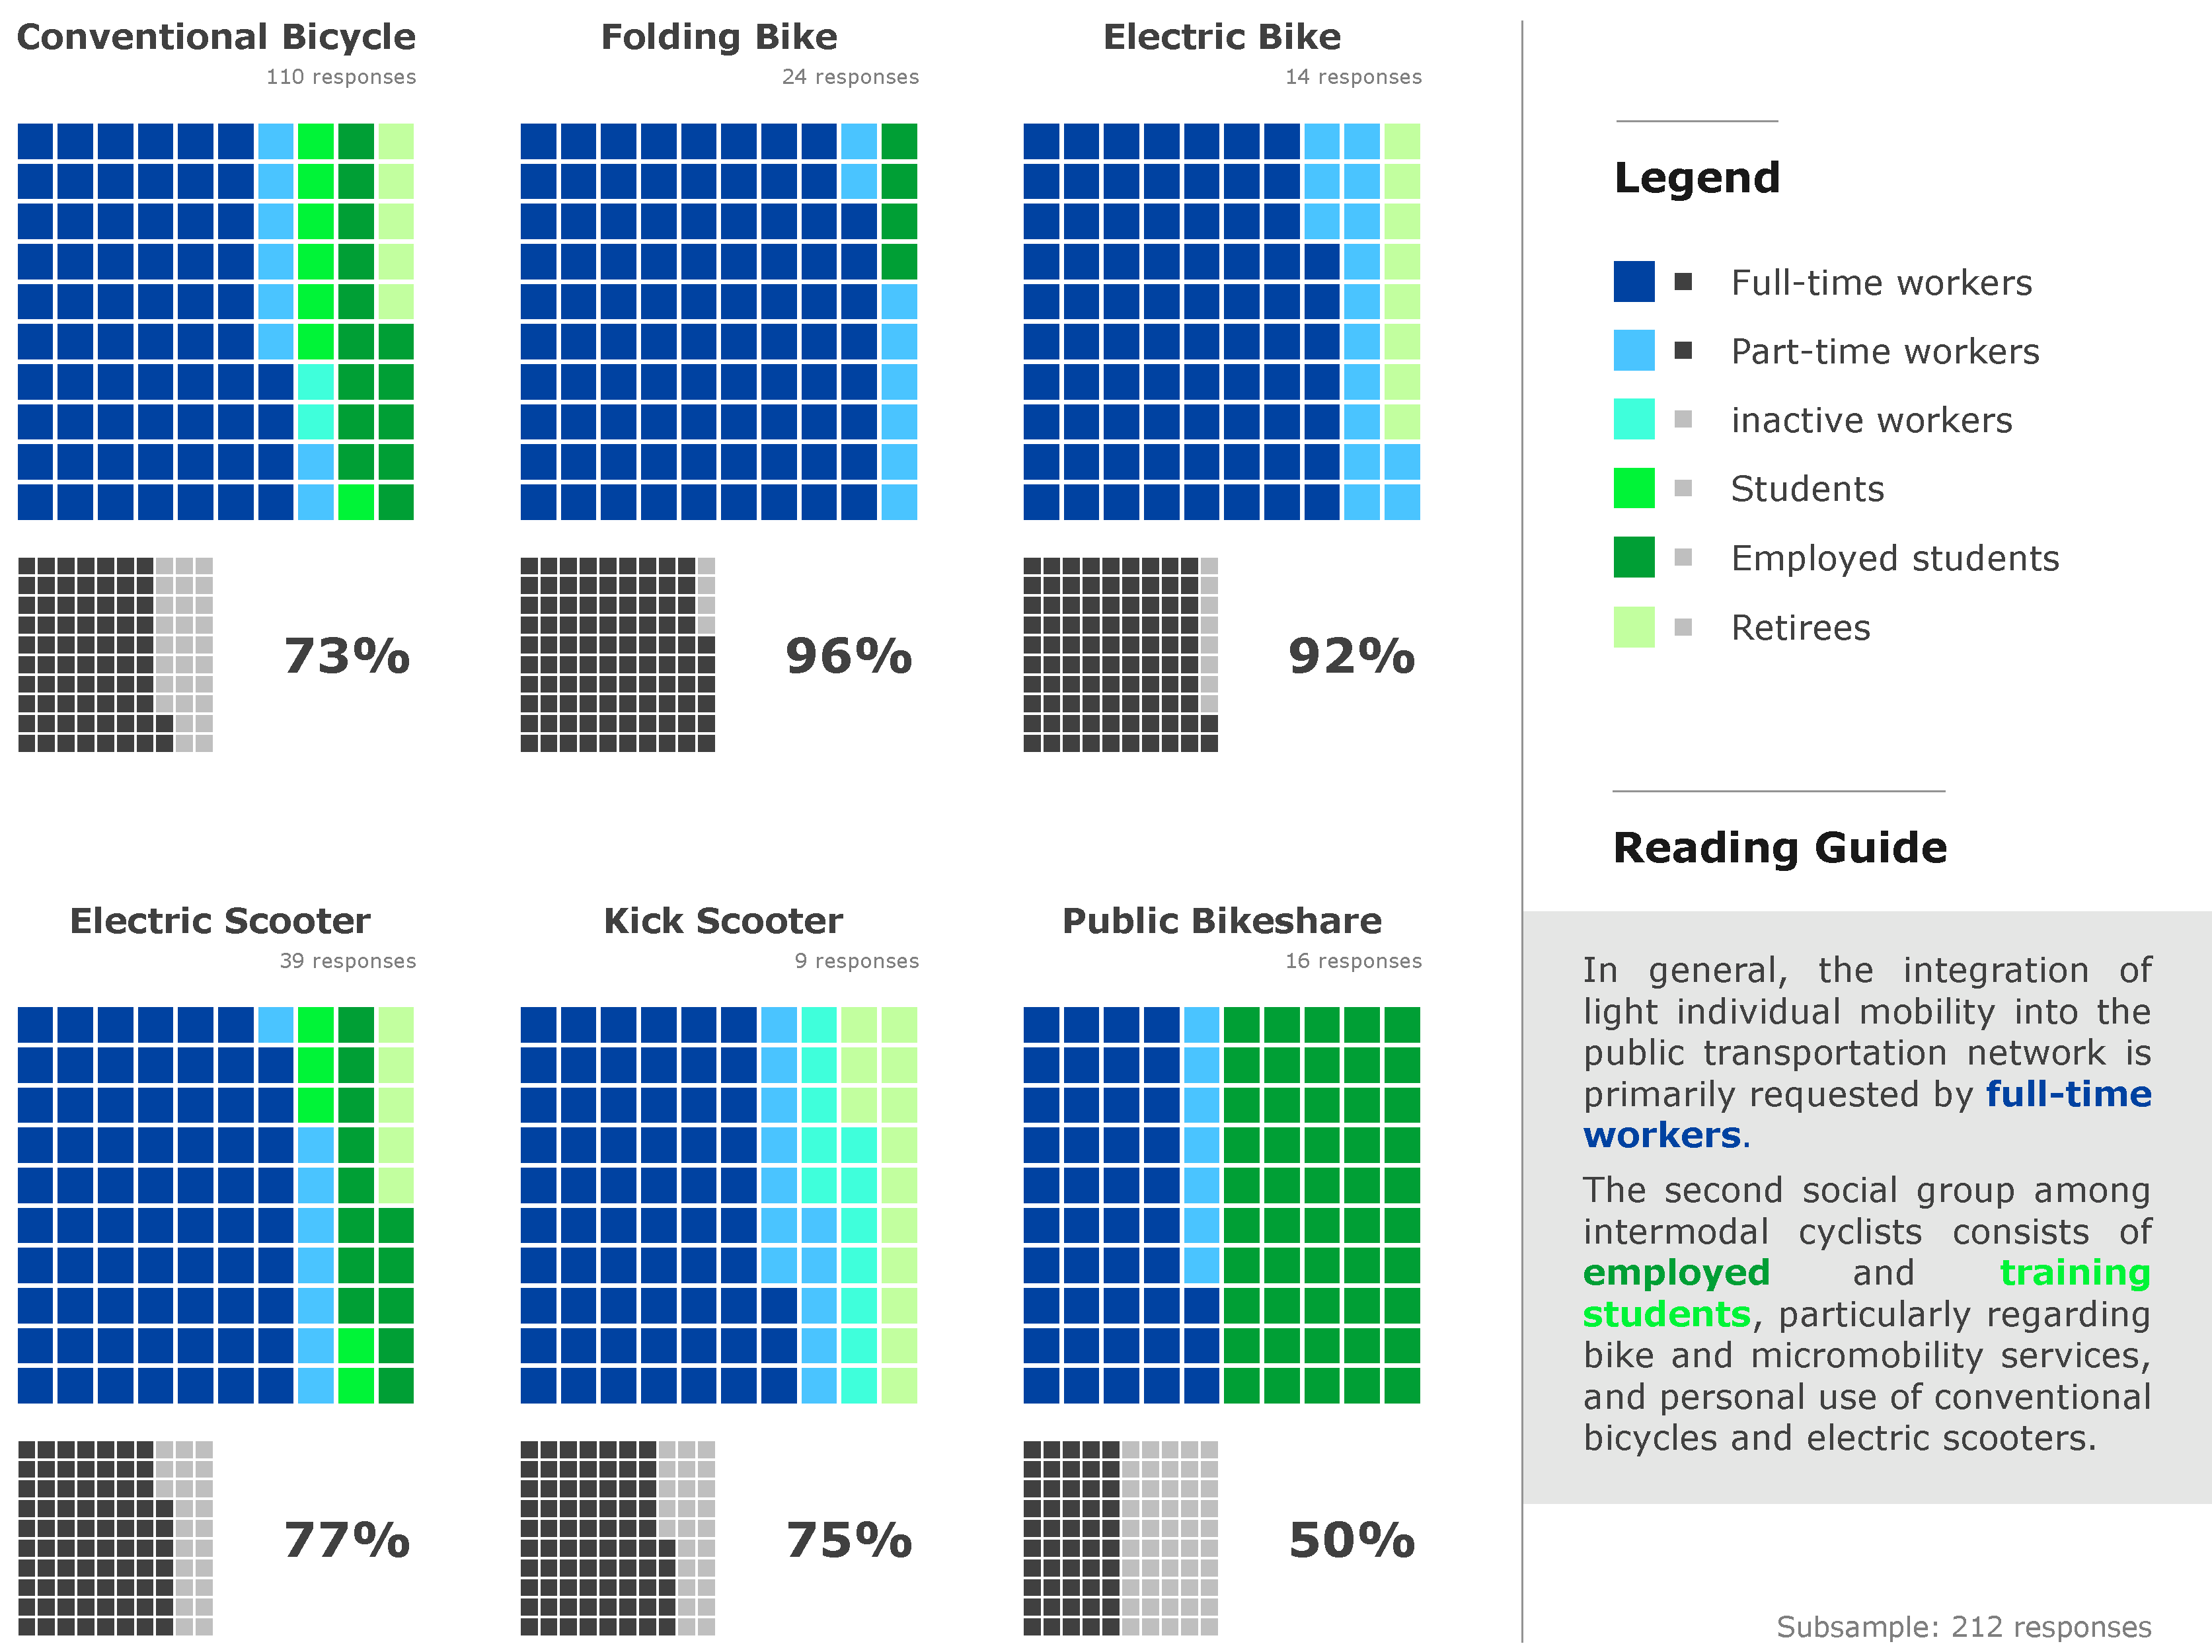
\includegraphics[width=1\columnwidth]{src/Figures/Chap-4/EN_Statut.pdf}}
        \vspace{5pt}
        \begin{flushleft}\scriptsize{
        Note: one \Commas{pixel} corresponds to 1\% of the analyzed subsample.
        }\end{flushleft}
        \begin{flushright}\scriptsize{
        Author: \textcolor{blue}{Dylan Moinse (2024)}
        }\end{flushright}
    \end{figure}

    % PCS - général
To explore in more detail the socio-professional dimension of cycle travelers, we included an additional question related to the \Commas{profession and socio-professional category [to which they currently belong or have recently belonged]} (see \hyperref[annexes:structure-questionnaire-usagers]{Appendix~\ref{annexes:structure-questionnaire-usagers}}, page~\pageref{annexes:structure-questionnaire-usagers}). Indeed, the notable presence of full-time employed individuals among these intermodal practices leads us to closely examine the social stratification within this population. The analysis of the \acrshort{PCS} shows a significant concentration of executives and higher intellectual professions, which represent 66\% of the active individuals in the questionnaire (109 responses). Employees form the second most represented group with 18\% (29 responses), while intermediate professions account for 9\% (15 responses). In contrast, craftsmen, traders, business owners, and workers each represent 4\% (6 responses), indicating a lower representation of these categories in the intermodal use of light mobility. In fact, the proportion of senior executives, already high among rail users, is even more significant in our survey of intermodal travelers. Conversely, professional categories such as workers and craftsmen are noticeably underrepresented (see \hyperref[table-chap4:capital-economique]{Table \ref{table-chap4:capital-economique}}, page~\pageref{table-chap4:capital-economique}).%%Translated%%

    % PCS - modes et transition
The targeted consideration of the proportion of executives and higher intellectual professions supports the hypothesis of their significant role in the intermodal use of light individual mobility (see \hyperref[fig-chap4:pcs]{Figure~\ref{fig-chap4:pcs}}, page~\pageref{fig-chap4:pcs}), and more particularly of folding bicycles (87\%, 19 responses). This trend continues with the \acrshort{e-Bike}, where 69\% of users belong to this category (9 responses), closely followed by traditional bicycles (69\%, 55 responses). In contrast, the proportion of these professions among \acrshort{PeS} users is less central, standing at 49\% (14 responses). It is noteworthy that the proportion of employees using \acrshort{PeS} is higher, reaching 31\% (9 responses). The clear presence of senior executives raises a broader question about household income, prompting us to adopt a perspective that goes beyond job classifications, in order to better understand the economic capital of intermodal users.%%Translated%%

    % Figure PCS
    \begin{figure}[h!]\vspace*{4pt}
        \caption{Professions and Socio-professional Categories of intermodal cyclists by type of vehicle.}
        \label{fig-chap4:pcs}
        \centerline{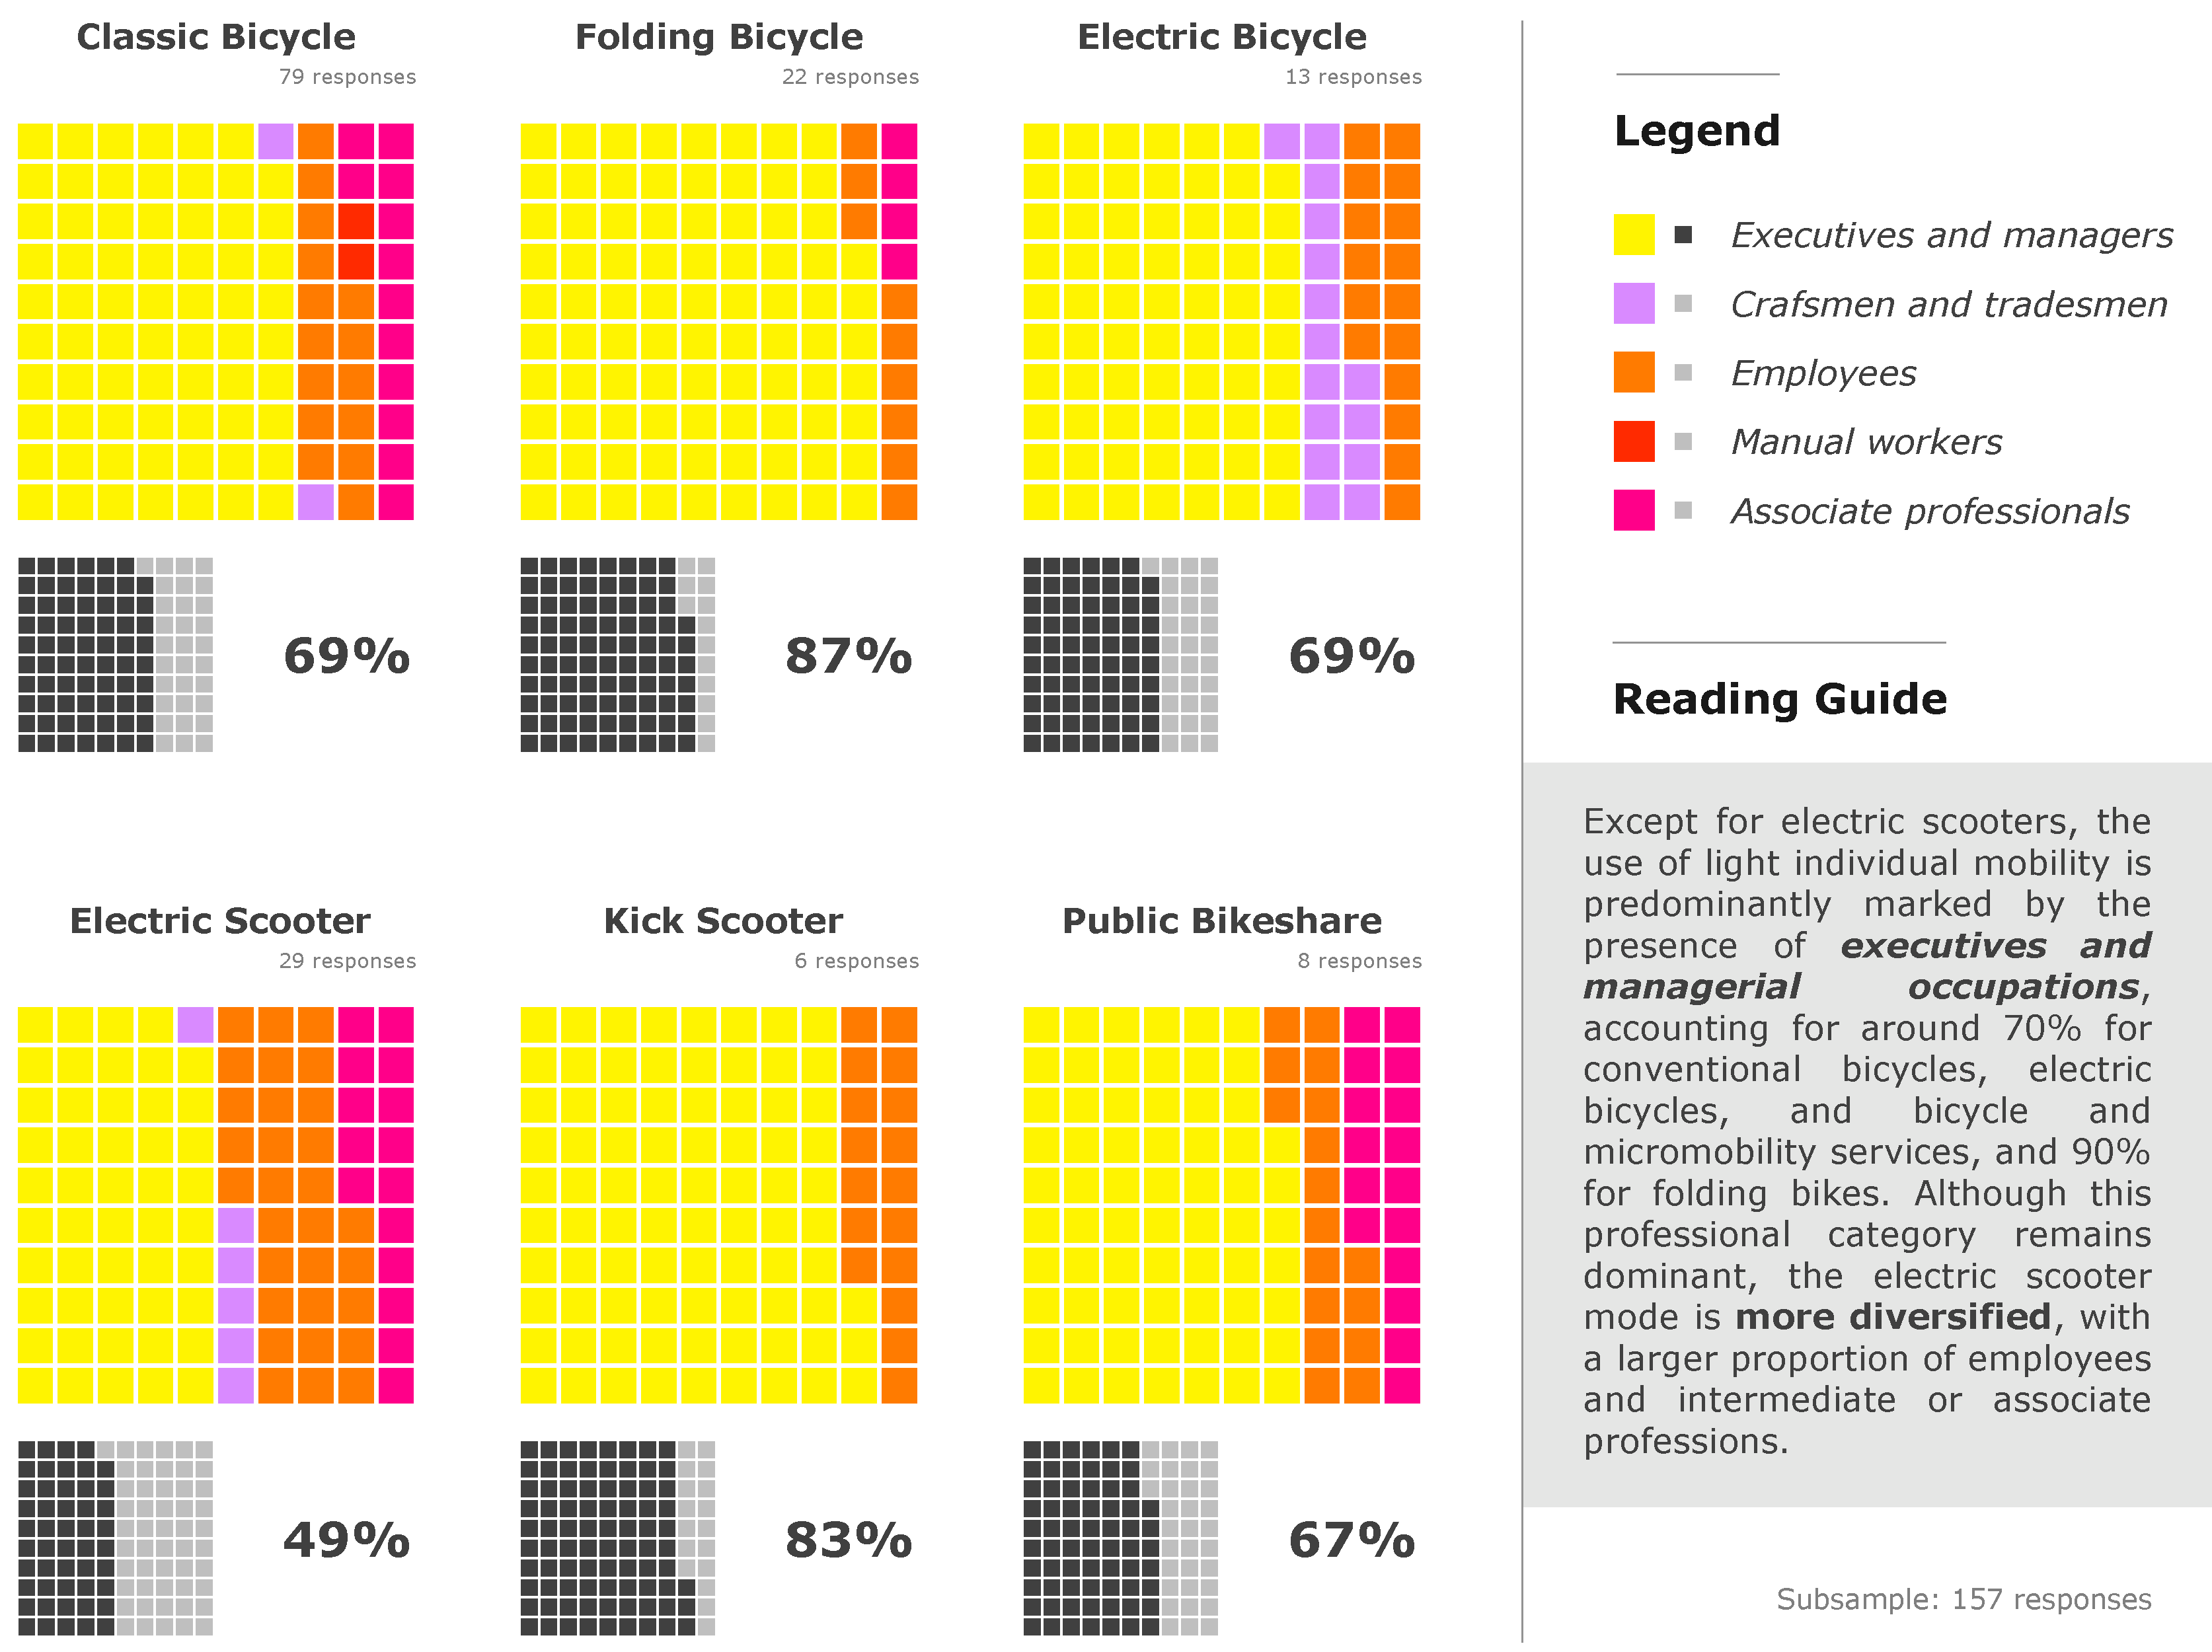
\includegraphics[width=1\columnwidth]{src/Figures/Chap-4/EN_PCS.pdf}}
        \vspace{5pt}
        \begin{flushleft}\scriptsize{
        Note: one \Commas{pixel} corresponds to 1\% of the analyzed subsample.
        }\end{flushleft}
        \begin{flushright}\scriptsize{
        Author: \textcolor{blue}{Dylan Moinse (2024)}
        }\end{flushright}
    \end{figure}

    % Littérature situation professionnelle + PCS + Transition
Particular attention has been paid to the professional situation of users of combined light individual mobility, showing a major influence of full-time employed individuals and students, while retirees are significantly underrepresented. This distribution, which is not representative of the French population, supports a body of international research that has highlighted a similarly unequal distribution \textcolor{blue}{\autocites[112]{quarshie_integrating_2007}[192]{sherwin_practices_2011}[21]{halldorsdottir_home-end_2017}{cervero_bike-and-ride_2013}[9]{jonkeren_bicycle-train_2021}[12]{pages_nouveaux_2021}}\index{Sherwin, Henrietta|pagebf}\index{Parkhurst, Graham|pagebf}\index{Robbins, Derek|pagebf}\index{Walker, Ian|pagebf}\index{Halldórsdóttir, Katrín|pagebf}\index{Nielsen, Otto Anker|pagebf}\index{Prato, Carlo Giacomo|pagebf}\index{Jonkeren, Olaf|pagebf}\index{Kager, Roland|pagebf}\index{Harms, Lucas|pagebf}\index{te Brömmelstroet, Marco|pagebf}\index{Quarshie, Magnus|pagebf}\index{Morrison, Gregory~M.|pagebf}\index{Rauch, Sébastien|pagebf}\index{Cervero, Robert|pagebf}\index{Caldwell, Benjamin|pagebf}\index{Cuellar, Jesus|pagebf}\index{Pages, Thibaud|pagebf}\index{Lammoglia, Adrien|pagebf}\index{Josselin, Didier|pagebf}. The preferred use of mobility services by students is also documented \textcolor{blue}{\autocites[215]{lin_built_2018}[8]{adnan_last-mile_2019}[3-4]{fearnley_patterns_2020}[12]{hu_examining_2022}[5]{cheng_comparison_2023}}\index{Lin, Jen-Jia|pagebf}\index{Zhao, Pengjun|pagebf}\index{Takada, Kazuyuki|pagebf}\index{Li, Shengxiao|pagebf}\index{Yai, Tetsuo|pagebf}\index{Chen, Chi-Hao|pagebf}\index{Adnan, Muhammad|pagebf}\index{Altaf, Shahbaz|pagebf}\index{Bellemans, Tom|pagebf}\index{Yasar, Ansar-ul-Haque|pagebf}\index{Shakshuki, Elhadi~M.|pagebf}\index{Hu, Songhua|pagebf}\index{Chen, Mingyang|pagebf}\index{Jiang, Yuan|pagebf}\index{Sun, Wei|pagebf}\index{Xiong, Chenfeng|pagebf}\index{Cheng, Long|pagebf}\index{Huang, Jie|pagebf}\index{Jin, Tanhua|pagebf}\index{Chen, Wendong|pagebf}\index{Li, Aoyong|pagebf}\index{Witlox, Frank|pagebf}\index{Fearnley, Nils|pagebf}\index{Johnsson, Espen|pagebf}\index{Berge, Siri Hegna|pagebf}.%%Translated%%

    % 4.2.1.2.
    \needspace{1\baselineskip} % Space reservation
\subsubsection*{Asymmetrically Distributed Incomes
    \label{chap4:capital-economique-revenu}
    }

    % Revenu brut - général
The question regarding the evaluation of monthly gross household income was asked. The \acrfull{GDI}\footnote{~
    The \acrfull{GDI} is an economic indicator reflecting the financial capacity of a household after direct taxes are paid and various public allowances and subsidies are integrated. This parameter includes not only the net monthly income from professional activity and owned assets, but also social benefits received. The \acrshort{GDI} thus provides a comprehensive view of the resources available to an individual or household, intended for consumption, investment, or savings.
} average for the respondents is~\euro3,058, while the median is~\euro2,850. This gap indicates the presence of relatively high incomes among the participants, contributing to an increase in the average. In comparison, this average salary is lower than the national average gross income of~\euro3,250; however, it exceeds the national median, which stands at~\euro2,250, as shown in the \hyperref[table-chap4:capital-economique]{Table~\ref{table-chap4:capital-economique}} (page~\pageref{table-chap4:capital-economique}). In the distributive analysis of incomes based on a cumulative series ranked by decile, it appears that the first quartile (\(Q1\)) places the income threshold for three-quarters of the respondents above~\euro1,750, while the third quartile (\(Q3\)) shows that a quarter of individuals earn more than~\euro4,050. This segmentation of the \acrshort{GDI} highlights a distribution unevenly weighted towards higher income brackets.%%Translated%%

    % Revenu brut - modes
The analysis of median incomes associated with the integration of light individual mobility reveals an overall median of~\euro2,850. However, marked disparities appear when we examine the data by mode of transport (see \hyperref[fig-chap4:revenus]{Figure~\ref{fig-chap4:revenus}}, page~\pageref{fig-chap4:revenus}). For example, folding bicycle users report a significantly higher median \acrshort{GDI}, reaching~\euro4,050 (24 responses), while \acrshort{e-Bike} users report~\euro3,400 (14 responses). In contrast, users of mechanical scooters and shared mobility systems have more modest median incomes, at~\euro2,625 (9 responses) and~\euro2,400 (16 responses), respectively. Traditional bicycles and \acrshort{PeS} fall into an intermediate range, with incomes aligned with the declared median. More broadly, the analysis of income distribution reveals a considerable gap between the lowest and highest income brackets, particularly for bike-sharing and traditional cycling.%%Translated%%

    % Figure Revenus
    \begin{figure}[h!]\vspace*{4pt}
        \caption{Boxplots of gross disposable income of intermodal cyclists by type of vehicle.}
        \label{fig-chap4:revenus}
        \centerline{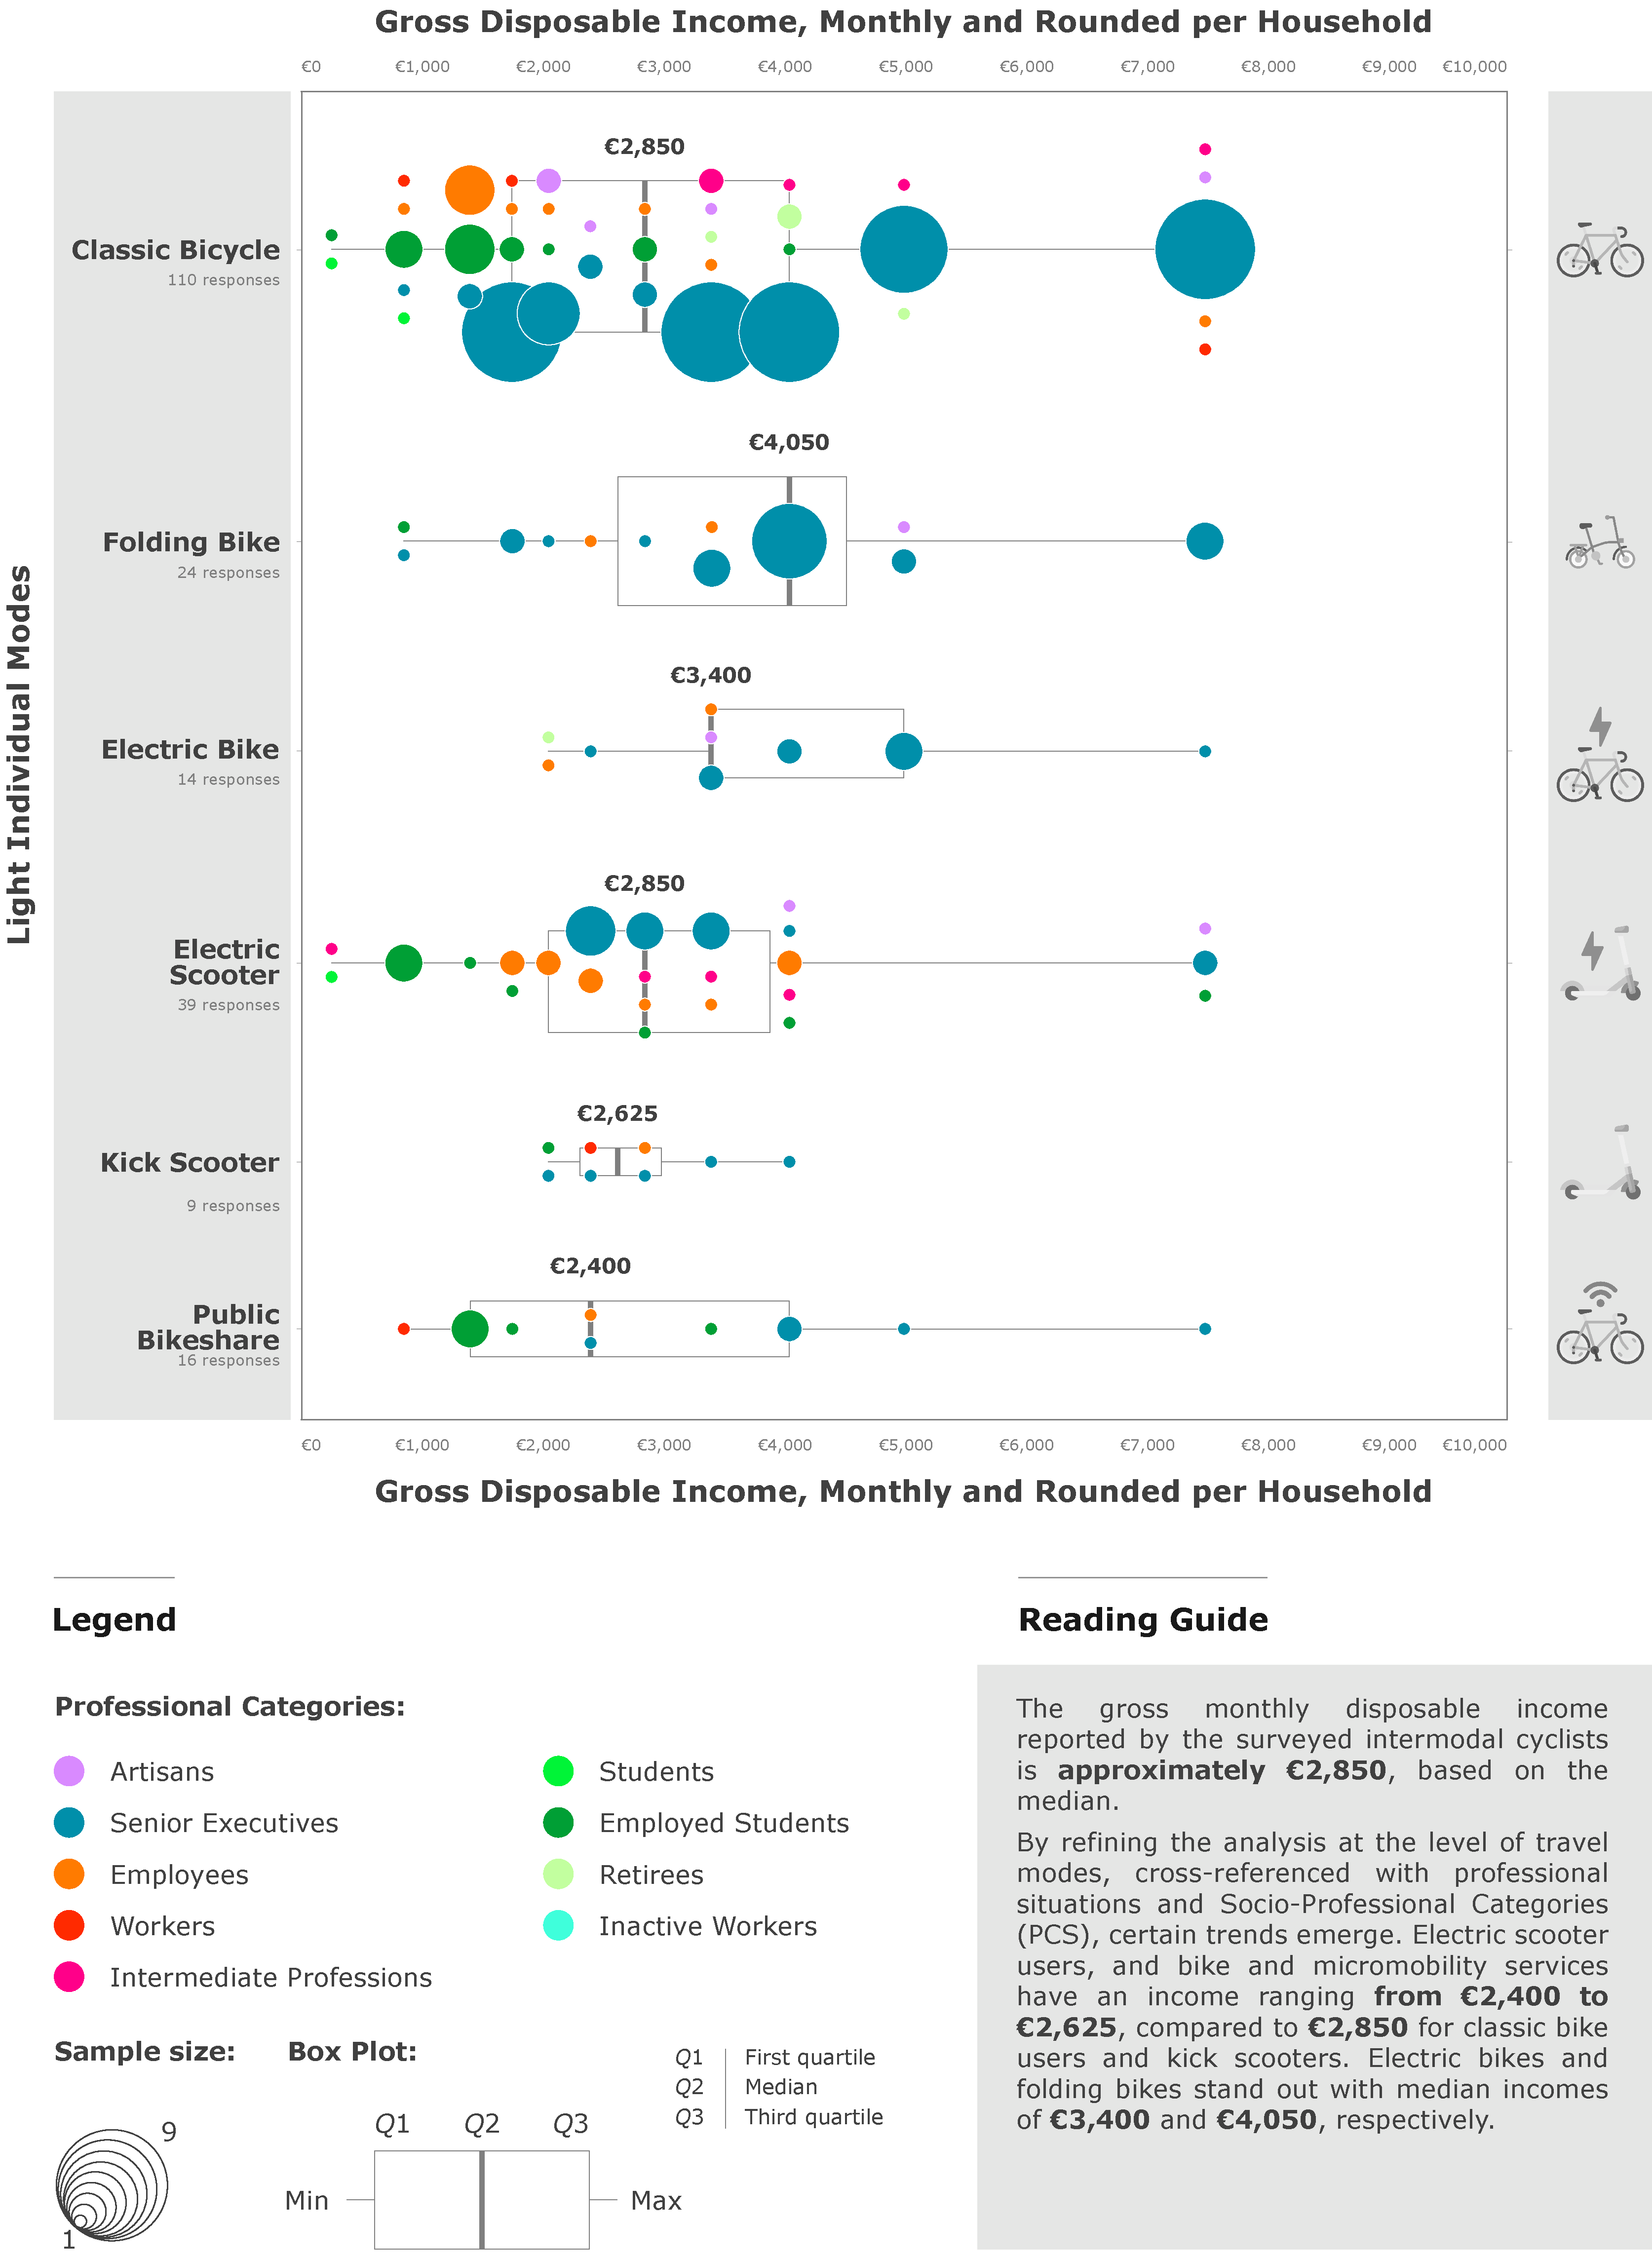
\includegraphics[width=1\columnwidth]{src/Figures/Chap-4/EN_Revenus.pdf}}
        \vspace{5pt}
        \begin{flushright}\scriptsize{
        Author: \textcolor{blue}{Dylan Moinse (2024)}
        }\end{flushright}
    \end{figure}

    % Littérature situation revenus + Transition
Particular attention has been given to the professional situation of users of combined light individual mobility, showing a major influence of full-time employed individuals and students, while retirees are significantly underrepresented. This distribution, which is not representative of the French population, supports a body of international research that has highlighted a similarly unequal distribution \textcolor{blue}{\autocites[112]{quarshie_integrating_2007}[192]{sherwin_practices_2011}[21]{halldorsdottir_home-end_2017}{cervero_bike-and-ride_2013}[9]{jonkeren_bicycle-train_2021}[12]{pages_nouveaux_2021}}\index{Sherwin, Henrietta|pagebf}\index{Parkhurst, Graham|pagebf}\index{Robbins, Derek|pagebf}\index{Walker, Ian|pagebf}\index{Halldórsdóttir, Katrín|pagebf}\index{Nielsen, Otto Anker|pagebf}\index{Prato, Carlo Giacomo|pagebf}\index{Jonkeren, Olaf|pagebf}\index{Kager, Roland|pagebf}\index{Harms, Lucas|pagebf}\index{te Brömmelstroet, Marco|pagebf}\index{Quarshie, Magnus|pagebf}\index{Morrison, Gregory~M.|pagebf}\index{Rauch, Sébastien|pagebf}\index{Cervero, Robert|pagebf}\index{Caldwell, Benjamin|pagebf}\index{Cuellar, Jesus|pagebf}\index{Pages, Thibaud|pagebf}\index{Lammoglia, Adrien|pagebf}\index{Josselin, Didier|pagebf}. The preferred use of mobility services by students is also documented \textcolor{blue}{\autocites[215]{lin_built_2018}[8]{adnan_last-mile_2019}[3-4]{fearnley_patterns_2020}[12]{hu_examining_2022}[5]{cheng_comparison_2023}}\index{Lin, Jen-Jia|pagebf}\index{Zhao, Pengjun|pagebf}\index{Takada, Kazuyuki|pagebf}\index{Li, Shengxiao|pagebf}\index{Yai, Tetsuo|pagebf}\index{Chen, Chi-Hao|pagebf}\index{Adnan, Muhammad|pagebf}\index{Altaf, Shahbaz|pagebf}\index{Bellemans, Tom|pagebf}\index{Yasar, Ansar-ul-Haque|pagebf}\index{Shakshuki, Elhadi~M.|pagebf}\index{Hu, Songhua|pagebf}\index{Chen, Mingyang|pagebf}\index{Jiang, Yuan|pagebf}\index{Sun, Wei|pagebf}\index{Xiong, Chenfeng|pagebf}\index{Cheng, Long|pagebf}\index{Huang, Jie|pagebf}\index{Jin, Tanhua|pagebf}\index{Chen, Wendong|pagebf}\index{Li, Aoyong|pagebf}\index{Witlox, Frank|pagebf}\index{Fearnley, Nils|pagebf}\index{Johnsson, Espen|pagebf}\index{Berge, Siri Hegna|pagebf}. Moreover, a notable positive association between travelers' income and their inclination to opt for light intermodal mobility has been highlighted, as shown by various studies \textcolor{blue}{\autocites[321]{martin_evaluating_2014}[172]{yang_bike-and-ride_2014}[8]{ma_bicycle_2015}[7]{yang_empirical_2016}[55]{zhao_bicycle-metro_2017}[216]{lin_built_2018}[378]{ravensbergen_biking_2018}[15]{shelat_analysing_2018}[399]{bocker_bike_2020}[2171]{chan_factors_2020}[184]{cao_e-scooter_2021}}\index{Shelat, Sanmay|pagebf}\index{Huisman, Raymond|pagebf}\index{Oort, Niels van|pagebf}\index{Chan, Kevin|pagebf}\index{Farber, Steven|pagebf}\index{Ravensbergen, Léa|pagebf}\index{Buliung, Ron|pagebf}\index{Mendonca, Meaghan|pagebf}\index{Garg, Naren|pagebf}\index{Yang, Liu|pagebf}\index{Chao, Li|pagebf}\index{Wang, Yuanqing|pagebf}\index{Martin, Elliot~W.|pagebf}\index{Shaheen, Susan~A.|pagebf}\index{Zhao, Pengjun|pagebf}\index{Li, Shengxiao|pagebf}\index{Yang, Min|pagebf}\index{Liu, Xinlu|pagebf}\index{Wang, Wei|pagebf}\index{Li, Zhibin|pagebf}\index{Zhao, Jingyao|pagebf}\index{Lin, Jen-Jia|pagebf}\index{Zhao, Pengjun|pagebf}\index{Takada, Kazuyuki|pagebf}\index{Li, Shengxiao|pagebf}\index{Yai, Tetsuo|pagebf}\index{Chen, Chi-Hao|pagebf}\index{Böcker, Lars|pagebf}\index{Anderson, Ellinor|pagebf}\index{Uteng, Tanu Priya|pagebf}\index{Throndsen, Torstein|pagebf}\index{Cao, Zhejing|pagebf}\index{Zhang, Xiaohu|pagebf}\index{Chua, Kelman|pagebf}\index{Yu, Honghai|pagebf}\index{Zhao, Jinhua|pagebf}\index{Ma, Ting|pagebf}\index{Liu, Chao|pagebf}\index{Erdoğan, Sevgi|pagebf}. More broadly, the overrepresentation of the aforementioned social groups is corroborated by \textcolor{blue}{\textcite[101]{dobruszkes_is_2022}}\index{Dobruszkes, Frédéric|pagebf}\index{Chen, Chia-Lin|pagebf}\index{Moyano, Amparo|pagebf}\index{Pagliara, Francesca|pagebf}\index{Endemann, Peter|pagebf}, who found that, for the \acrshort{HST} in France, a significant majority of users are senior executives and high-income individuals, particularly on the Northern segment connecting the Hauts-de-France. Additionally, a high level of education among \acrshort{HST} travelers suggests a strong association between profession type, income, and education level among cycle travelers, as highlighted by \textcolor{blue}{\textcite[86]{zuo_incorporating_2021}}\index{Zuo, Ting|pagebf}\index{Wei, Heng|pagebf}\index{Chen, Na|pagebf}. Thus, this section dealing with economic capital invites us to consider the cultural capital of these individuals, in order to refine the determination of the socio-demographic profile of the intermodal users surveyed.%%Translated%%

    % 4.2.1.3.
    \needspace{1\baselineskip} % Space reservation
\subsubsection*{A Highly Qualified Social Group
    \label{chap4:capital-culturel}
    }

    % Niveau de diplômes - général
Based on the question regarding the highest degree obtained, we can estimate the cultural capital of travelers using bicycles or micromobility. According to the survey, more than 95\% of respondents hold a higher education degree, which is significantly above the national average of 43\% (see \hyperref[table-chap4:capital-culturel]{Table~\ref{table-chap4:capital-culturel}}, page~\pageref{table-chap4:capital-culturel}). About 49\% of respondents have at least a Master's degree, levels $7$ and $8$ according to the \acrfull{RNCP}\footnote{~
    The \acrfull{RNCP} is an official register listing qualifications and certifications, accessible through vocational training, that are recognized by the state. These qualifications are classified by level, ranging from level $3$ for \acrshort{CAP} or \acrshort{BEP} to level $8$ for a PhD and \acrshort{HDR}.
}, compared to only 9.40\% on average for the entire French population. Furthermore, while 13\% of the French population has no diploma or primary school certificate, this proportion drops to 1\% among the intermodal travelers concerned, highlighting their strong educational capital.%%Translated%%

    % Niveau de diplômes - modes
The profile of users is marked by different education levels across the vehicles studied. While 86\% of respondents hold a bachelor's, master's, or doctoral degree (levels $6$ to $8$, 180 responses), 96\% of folding bicycle users have one of these degrees (23 responses), compared to 89\% for traditional bicycles (93 responses) and 74\% for \acrshort{PeS} (29 responses). The electric vehicle category indeed has a higher proportion of users with a \acrshort{BTS}, \acrshort{DEUG}, \acrshort{DEUST}, \acrshort{DUT}, or high school diploma as their highest level of education.%%Translated%%

    % Tableau Capital culturel
% Table Cultural Capital
%%Rédigé%%
    \begin{table}[h!]
    \centering
    \renewcommand{\arraystretch}{1.5}
    \resizebox{\columnwidth}{!}{
    \begin{tabular}{p{0.13\columnwidth}p{0.61\columnwidth}p{0.13\columnwidth}p{0.13\columnwidth}}
        %\hline
    \rule{0pt}{15pt} \small{\textcolor{blue}{{\textbf{Level}}}} & \small{\textcolor{blue}{{\textbf{Degree}}}} & \small{\textcolor{blue}{{\textbf{Survey}}}} & \small{\textcolor{blue}{{\textbf{France}}}}\\
        \hline
\small{-} & \small{No degree or primary school certificate} & \small{\textbf{0.96\%}} & \small{12.50\%}\\
\small{-} & \small{Diploma of the French middle school (Brevet des collèges)} & \small{\textbf{0.48\%}} & \small{3.80\%}\\
\small{$3$} & \small{\acrshort{CAP} or \acrshort{BEP}} & \small{\textbf{0.48\%}} & \small{22.40\%}\\
\small{$4$} & \small{Baccalaureate} & \small{\textbf{3.35\%}} & \small{18.80\%}\\
\small{$5$} & \small{\acrshort{BTS}, \acrshort{DEUG}, \acrshort{DEUST}, or \acrshort{DUT}} & \small{\textbf{8.61\%}} & \small{14.30\%}\\
\small{$6$} & \small{Bachelor's, professional bachelor's, \acrshort{BUT}, or Master's degree} & \small{\textbf{36.84\%}} & \small{18.80\%}\\
\multirow{1.5}{*}{\small{$7$}} & \small{Master's, advanced studies diploma, specialized studies diploma, or engineering degree} & \multirow{1.5}{*}{\small{\textbf{47.85\%}}} & \multirow{1.5}{*}{\small{8.30\%}}\\
\small{$8$} & \small{Doctorate or \acrshort{HDR}} & \small{\textbf{1.44\%}} & \small{1.10\%}\\
        \hline
        \end{tabular}}
    \caption{Qualification level of intermodal cyclists.}
    \label{table-chap4:capital-culturel}
        \vspace{5pt}
        \begin{flushleft}\scriptsize
        \textcolor{blue}{Reading Guide:} Compared to the national average, users are much more highly educated, with a predominance of those holding a Bachelor's or Master's degree.
        \end{flushleft}
        \begin{flushright}\scriptsize{
        Datasets: \textcolor{blue}{\textcite{insee_niveau_2021}}\index{Insee@\textsl{Insee}|pagebf}
        \\
        Author: \textcolor{blue}{Dylan Moinse (2024)}
        }\end{flushright}
        \end{table}%%Rédigé%%

    % Littérature diplômes + transition
The predominance of graduates among users of light individual mobility in intermodality is confirmed by existing literature, which frequently associates a high level of education with the adoption of these intermodal practices. Nearly 86\% of the participants in our study hold a higher education degree, a figure that aligns with the 85\% measured by \textcolor{blue}{\textcite[15]{shelat_analysing_2018}}\index{Shelat, Sanmay|pagebf}\index{Huisman, Raymond|pagebf}\index{Oort, Niels van|pagebf}, \textcolor{blue}{\textcite[113]{heinen_multimodal_2014}}\index{Heinen, Eva|pagebf}\index{Bohte, Wendy|pagebf}, and \textcolor{blue}{\textcite[11]{jonkeren_bicycle-train_2021}}\index{Jonkeren, Olaf|pagebf}\index{Kager, Roland|pagebf}\index{Harms, Lucas|pagebf}\index{te Brömmelstroet, Marco|pagebf} in the Netherlands, as well as the 75\% and 74\% reported respectively by \textcolor{blue}{\textcite[6, 8]{adnan_last-mile_2019}}\index{Adnan, Muhammad|pagebf}\index{Altaf, Shahbaz|pagebf}\index{Bellemans, Tom|pagebf}\index{Yasar, Ansar-ul-Haque|pagebf}\index{Shakshuki, Elhadi~M.|pagebf} in Belgium and by \textcolor{blue}{\textcite[103]{flamm_public_2014}}\index{Flamm, Bradley~J.|pagebf}\index{Rivasplata, Charles~R.|pagebf} in the United States. In comparison with rail travelers in France, where 63\% of individuals hold an education level higher than the baccalaureate, it is clear that the educational capital of intermodal cyclists is significantly higher, even surpassing that of \acrshort{HST} users in France, where the rate is 70\%.%%Translated%%

    % Transition
The entry through economic capital highlights a clear overrepresentation of full-time employed individuals, particularly senior executives with relatively high incomes, among cycle travelers. This observation aligns with the social representations conveyed: that of the cyclist taking the train and coming from a privileged socio-professional category. Beyond the cycling and rail accessibility offered by the examined modal combinations, it is also important to investigate the mobility capabilities of these users, namely the possession of mobility equipment and their travel habits.%%Translated%%

    % 4.2.3.
    \needspace{1\baselineskip} % Space reservation
\subsection{Multimodal Profile: Between Two-Wheels and Four-Wheels
    \label{chap4:capital-mobilite}
    }

    % Introduction
The analysis of the mobility profile of cycle travelers aims to support the diversity of their mobility capital, that is, the material resources and mobility practices they have on a daily basis. This section first focuses on the possession of vehicles within the households of these users to determine whether they benefit from mobility flexibility, beyond intermodal alternatives. In addition, we will explore their travel habits to see if they lean towards multimodal practices or if they restrict themselves to the intermodal use of mobility in their daily and occasional travels.%%Translated%%

    % 4.2.3.1.
    \needspace{1\baselineskip} % Space reservation
\subsubsection*{An Overrepresentation of Motorized Households
    \label{chap4:capital-mobilite-equipement}
    }

    % Equipement en vélo
Among the survey respondents, 73\% own at least one bicycle. Excluding those who use a personal bicycle for the questionnaire, we observe that 47\% of users report owning one (50 responses). To put this in context, in 2019, about 32\% of French households had at least one adult bicycle used in the past year, according to data from \textcolor{blue}{\textcite{commissariat_general_au_developpement_durable_combien_2022}}\index{Commissariat général au développement durable@\textsl{Commissariat général au développement durable}|pagebf}. Thus, intermodal cyclists tend to be more frequently equipped with a bicycle. For example, among \acrshort{PeS} users, 46\% also own a bicycle (18 responses). This suggests that, even when owning a bicycle, these individuals prefer using \acrshort{PMD} for their intermodal trips. Furthermore, half of the users of a shared bicycle or scooter also own one (7 responses), suggesting that they opt for this sharing system to facilitate their connection to public transport hubs (see \hyperref[fig-chap4:equipement]{Figure~\ref{fig-chap4:equipement}}, page~\pageref{fig-chap4:equipement}).%%Translated%%

    % Taux de motorisation
The examination of mobility equipment among respondents reveals a motorization rate of 69\% (149 responses), a level similar to that observed in France, estimated at about 600 vehicles per 1,000 inhabitants \textcolor{blue}{\autocite{insee_equipement_2020}}\index{Insee@\textsl{Insee}|pagebf}. This rate varies depending on the mode of transport used (see \hyperref[fig-chap4:equipement]{Figure~\ref{fig-chap4:equipement}}, page~\pageref{fig-chap4:equipement}). Shared mobility users exhibit the lowest motorization rate, at 60\% (9 responses), followed by traditional bicycles at 65\% and folding bicycles at 71\% (72 and 17 responses). In contrast, users of \acrshort{PeS} and \acrshort{e-Bike}, whether folding or not, show some of the highest motorization rates, reaching 77\% for each of these modes (30 and 10 responses). These figures are still higher than those observed by \textcolor{blue}{\textcite[362]{givoni_access_2007}}\index{Givoni, Moshe|pagebf}\index{Rietveld, Piet|pagebf} and \textcolor{blue}{\textcite[7]{yang_empirical_2016}}\index{Yang, Min|pagebf}\index{Liu, Xinlu|pagebf}\index{Wang, Wei|pagebf}\index{Li, Zhibin|pagebf}\index{Zhao, Jingyao|pagebf}, at 49\%.%%Translated%%

    % Figure Equipement
    \begin{figure}[h!]\vspace*{4pt}
        \caption{Equipment of intermodal cyclists, in bicycles and cars, by type of vehicle.}
        \label{fig-chap4:equipement}
        \centerline{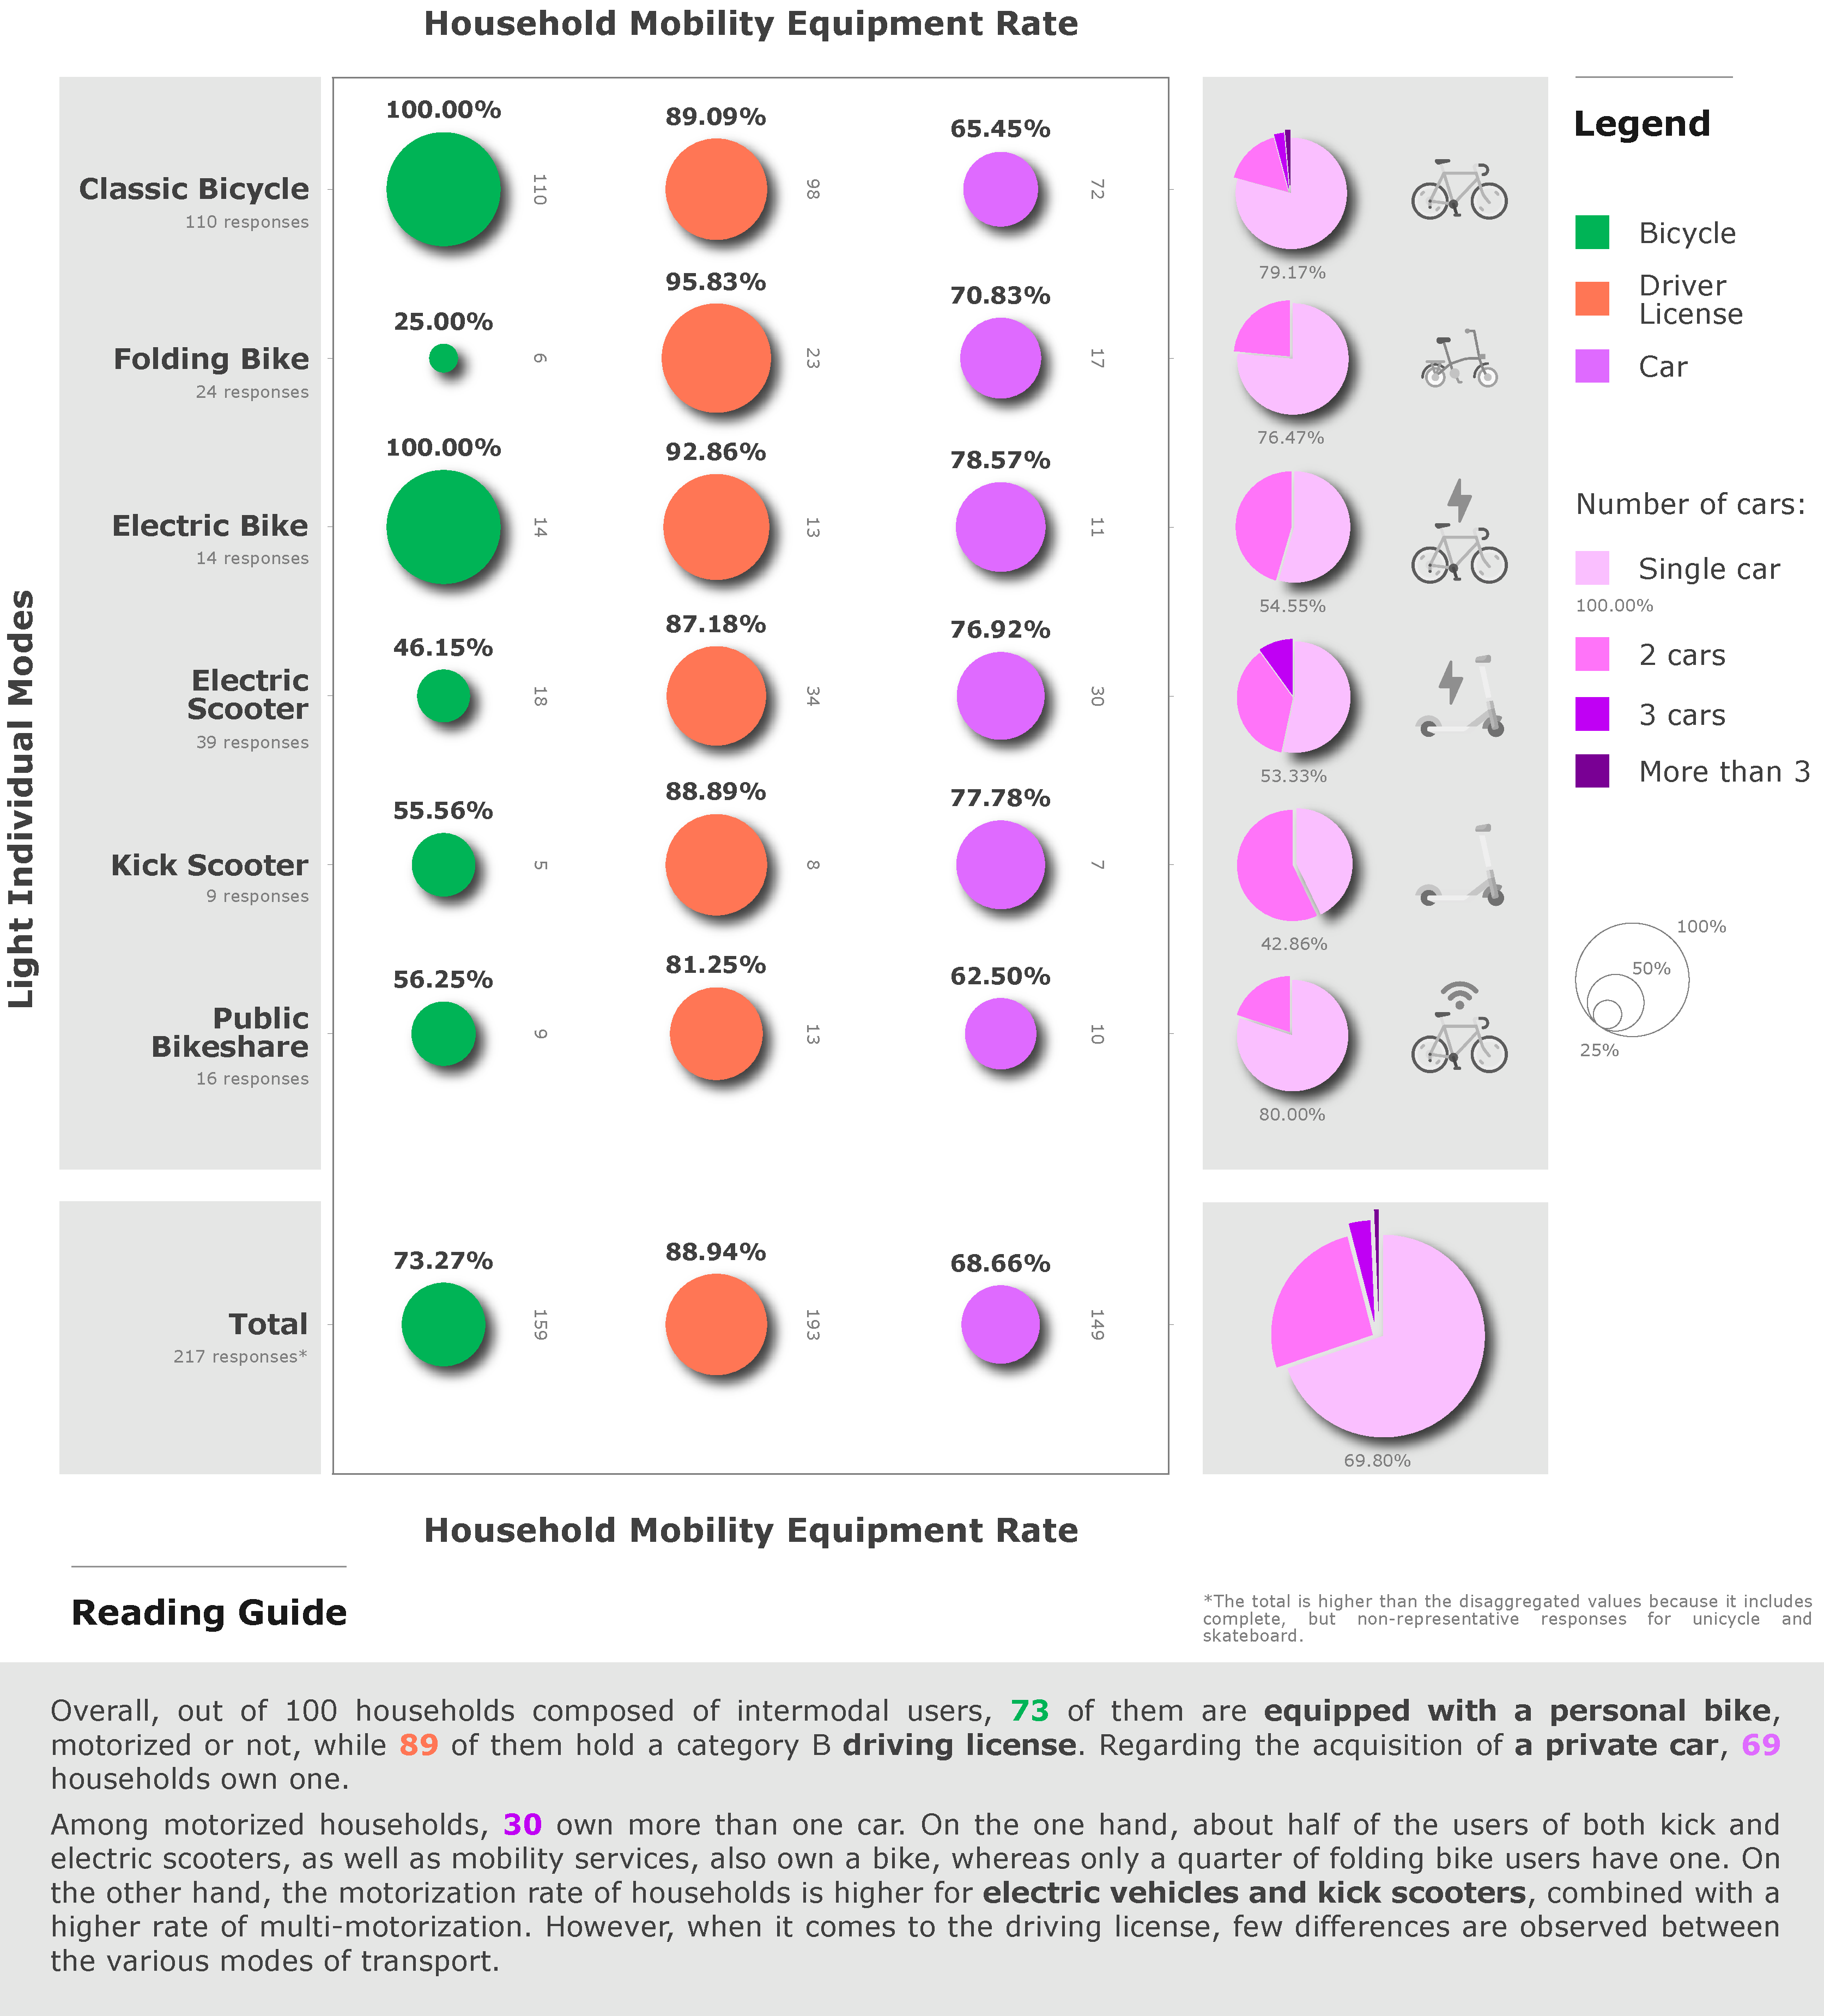
\includegraphics[width=1\columnwidth]{src/Figures/Chap-4/EN_Taux_motorisation.pdf}}
        \vspace{5pt}
        \begin{flushright}\scriptsize{
        Author: \textcolor{blue}{Dylan Moinse (2024)}
        }\end{flushright}
    \end{figure}

    % Nombre de voitures
In a more detailed exploration of the data, it appears that, for all cycle travelers, the average number of cars per household is 0.93, while those who are motorized own an average of 1.35 vehicles (see \hyperref[fig-chap4:equipement]{Figure~\ref{fig-chap4:equipement}}, page~\pageref{fig-chap4:equipement}). Among these motorized individuals, 30\% own more than one car (45 responses), and 4\% own three or more cars (6 responses). Thus, the proportion of 34\% of survey participants owning multiple vehicles is quite close to the equipment rate of the French population in 2018, which stands at 36\% for multi-motorized households \textcolor{blue}{\autocite{insee_equipement_2020}}\index{Insee@\textsl{Insee}|pagebf}. In this regard, \textcolor{blue}{\textcite[22]{cheng_expanding_2018}}\index{Cheng, Yung-Hsiang|pagebf}\index{Li, Yi-Chun|pagebf} distinguish between owners of a single car, who tend to be more regular users of \acrshort{PBS}, and those with multiple vehicles who are less likely to adopt these intermodal practices. Among the motorized cyclists surveyed, 21\% of traditional bike users and 24\% of folding bike users are equipped with at least two motorized vehicles (15 and 4 responses). However, the situation differs for electric mobility: 47\% of users with a \acrshort{PeS} and 50\% with a \acrshort{e-Bike} are multi-equipped (14 and 5 responses). This gap could indicate that electric light individual mobility is favored by motorized households, willing to travel on the road network and sharing common values\footnote{~
    Some studies show that bicycles and scooters share several values associated with \Commas{automobility} \textcolor{blue}{\autocites[57-58]{urry_sociology_2000}[28]{urry_system_2004}}\index{Urry, John|pagebf}, including the sense of freedom, flexibility, and independence, as well as technical elements such as infrastructure, which characterize car driving. These material and symbolic resources particularly appeal to car owners who wish to maintain these advantages. Light individual mobility thus ensures an excellent potential for modal shift by guaranteeing a transition towards a \Commas{velomobility} system \textcolor{blue}{\autocite[492]{watson_how_2012}}\index{Watson, Matt|pagebf}.
}, either to replace the car in intermodal uses or because electric vehicles fail to discourage these households from retaining access to a private car.%%Translated%%

    % Permis de conduire
To explore this hypothesis, our survey included a question about the possession of a driving license, cross-referenced with the motorization rate, to identify the profiles of drivers, whether they are regular, occasional, or potential drivers (see \hyperref[fig-chap4:equipement]{Figure~\ref{fig-chap4:equipement}}, page~\pageref{fig-chap4:equipement}). Overall, a large majority of respondents, 89\%, hold a valid category B driving license\footnote{~
    The category B driving license is the most common license, allowing the holder to drive private cars and other light vehicles weighing no more than 3.5 tons and carrying up to 8 passengers.
} (193 responses). The proportion of driving license holders among rail travelers who use bicycles and micromobility is significantly higher than within the French population of driving age, standing at about 76\%. This finding aligns with the tendency observed in other regions for driving license holders to shift more towards intermodal bicycle use, both for owned and shared bikes \textcolor{blue}{\autocites[111]{bachand-marleau_much-anticipated_2011}[215]{lin_built_2018}[7]{hamidi_shaping_2020}}\index{Hamidi, Zahra|pagebf}\index{Zhao, Chunli|pagebf}\index{Lin, Jen-Jia|pagebf}\index{Zhao, Pengjun|pagebf}\index{Takada, Kazuyuki|pagebf}\index{Li, Shengxiao|pagebf}\index{Yai, Tetsuo|pagebf}\index{Chen, Chi-Hao|pagebf}\index{Bachand-Marleau, Julie|pagebf}\index{Larsen, Jacob|pagebf}\index{El-Geneidy, Ahmed~M.|pagebf}. Among the 68 non-motorized participants, 52 still hold this license. Conversely, among the 149 individuals who own a motorized vehicle, 8 do not have a license, which may indicate the use of the vehicle by other household members or potential automobile use as a passenger (\textsl{kiss-and-ride}). We must remain cautious with this assumption, as our questionnaire did not ask whether respondents had access to a car. Given the links between intermodal use of light individual mobility and car ownership, we will further investigate the mobility practices of cycle travelers to assess the extent to which these users adopt multimodal behavior or whether they exclusively engage in intermodal use of light individual mobility for both their daily and occasional trips.%%Translated%%

    % 4.2.3.2.
    \needspace{1\baselineskip} % Space reservation
\subsubsection*{\textsl{Pedaling}, \textsl{Walking}, and \textsl{Driving}
    \label{chap4:capital-mobilite-habitudes}
    }

    % Habitudes de mobilité
By examining the mobility habits of participants using a scale ranging from \Commas{daily} to \Commas{never} for each mode of transport, we find that most adopt a multimodal approach. Thus, in their daily mobility, 83\% of respondents regularly walk (180 responses), 21\% drive a car (46 responses), and 4\% are passengers in a car (8 responses). For occasional trips, 12\% of respondents walk (25 responses), while car use reaches 27\% as drivers (59 responses) and 25\% in \textsl{kiss-and-ride} mode (55 responses). Scooters and motorcycles, like taxis and \acrshort{RHS}, are used by 3\% of individuals each, totaling 12 responses. Focusing on the specific habits of motorized cycle travelers, we observe that 7\% use their car \Commas{daily} (11 responses), 22\% \Commas{regularly} (34 responses), 37\% \Commas{occasionally} (57 responses), 22\% \Commas{rarely} (34 responses), and 11\% \Commas{never} (17 responses).%%Translated%%

    % Discussion
This distribution in the frequency of use of different modes of transport, coexisting with light individual mobility and public transport, demonstrates how intermodal users do not observe these mobility practices exclusively, but tend to regularly prioritize walking and occasionally use a car. This portrait of users combining light individual mobility and public transport, while also cultivating other mobility practices, may allude to the thesis of \Commas{multimodalization} of behaviors developed by \textcolor{blue}{Anaïs} \textcolor{blue}{\textcite[16]{rocci_automobilite_2007}}\index{Rocci, Anaïs|pagebf}. This approach has the merit of going beyond the simple notion of modal shift, which is difficult to apply to cycle travelers who are also occasional car users. It echoes the prospective exercise of \textcolor{blue}{Zygmunt} \textcolor{blue}{\textcite[7-28]{bauman_liquid_2000}}\index{Bauman, Zygmunt|pagebf}, who compares contemporary societies to the image of \Commas{liquid life} (\textsl{liquid modernity}), characterized by life rhythms marked by perpetual motion and flexibility, symbols of individual freedom, and opposed to the idea of rigid services. In this regard, it is less about a transition to a system of \Commas{velomobility} \textcolor{blue}{\autocite[492]{watson_how_2012}}\index{Watson, Matt|pagebf} than a shift from a system of \Commas{automobility} \textcolor{blue}{\autocites[57-58]{urry_sociology_2000}[28]{urry_system_2004}}\index{Urry, John|pagebf} to one of \Commas{multimobility}\footnote{~
    Multimobility refers to the use of various modes of transport to move around \textcolor{blue}{\autocite[10]{rocci_automobilite_2007}}\index{Rocci, Anaïs|pagebf}, a concept similar to comodality, introduced by the \textcolor{blue}{\textcite[6]{parlement_europeen_pour_2007}}\index{Parlement européen@\textsl{Parlement européen}|pagebf} in its transport policies, to be distinguished from intermodality. Multimobility emphasizes the flexibility and adaptability of individuals who opt for various mobility solutions to optimize their journeys.
}.%%Translated%%

    % Transition
The analysis revealed that cycle travelers not only benefit from high economic capital and a privileged social status, but also possess a certain adaptability in their mobility choices, partly enabled by owning motor vehicles. However, the integration of light individual mobility is also influenced by demographic factors such as age and gender, which limit the range of possibilities in terms of mobility. By studying accessibility through the lens of social inclusivity as an analytical framework, we will now examine disparities in mobility access for this social group through the prism of its demographics.%%Translated%%

    % 4.2.3.
    \needspace{1\baselineskip} % Space reservation
\subsection{The Intermodal Traveler, a Typical Portrait of the \textsl{Young Adult Man}
    \label{chap4:demographie}
    }

    % Amorce
The commercialization of kick scooters, followed by the advent of electric models, led to the development of sales strategies targeting an adult and female clientele. In this regard, advertising campaigns from the early 20\textsuperscript{st} century worked to transform the representation of the scooter as a leisure object, primarily intended for children, into a tool for women's emancipation, contributing to their daily mobility \textcolor{blue}{\autocite{hemmings_look_2011}}\index{Hemmings@\textsl{Hemmings}|pagebf}. This evolution echoes the movements for individual freedoms that, at the turn of the century, used the bicycle as a symbol of women's empowerment \textcolor{blue}{\autocite[187]{heran_retour_2015}}\index{Héran, Frédéric|pagebf}. It is now recognized that the use of electric scooters, like bicycles, is characterized by a dual effect of age and gender. At the same time, some studies raise the question of the exacerbation of socio-demographic inequalities with the development of \acrshort{PeS}, although \textcolor{blue}{\textcite[12]{curl_same_2020}}\index{Curl, Angela|pagebf}\index{Fitt, Helen|pagebf} bring nuance to the analysis, showing that micromobility manages to attract a demographically more diverse audience than that of bicycles.%%Translated%%

    % Introduction
Scientific and technical literature widely recognizes an unequal distribution of the monomodal use of light individual mobility, particularly in terms of the demographic characteristics of users in Europe and North America \textcolor{blue}{\autocites[101]{handy_factors_2011}[8]{codina_built_2022}}\index{Handy, Susan~L.|pagebf}\index{Xing, Yan|pagebf}\index{Codina, Oriol|pagebf}\index{Maciejewska, Monika|pagebf}\index{Nadal, Jordi|pagebf}\index{Marquet, Oriol|pagebf}. Studies indicate that the distribution by age and gender in bicycle use is significantly imbalanced, reflecting marked disparities, unlike walking and public transport usage where women are more represented \textcolor{blue}{\autocite[5-7]{pollard_gender_2017}}\index{Pollard, Tessa~M.|pagebf}\index{Wagnild, Janelle~M.|pagebf}. However, these social inequalities are less pronounced in some Nordic countries such as the Netherlands, Denmark, and Germany, where a well-established cycling culture has allowed for greater parity \textcolor{blue}{\autocites[81]{nelson_if_1997}[505]{pucher_making_2008}}\index{Nelson, Arthur~C.|pagebf}\index{Allen, David|pagebf}. Japan also constitutes an exception, with a wider adoption of cycling by women, reflecting specific socio-cultural norms \textcolor{blue}{\autocite[21-22]{lagadic_cycling_2022}}\index{Lagadic, Marion|pagebf}.%%Translated%%

    % Objectifs
However, in regions where bicycle use is lower, young men tend to use it more frequently than women, as seen in Barcelona \textcolor{blue}{\autocite[7]{codina_built_2022}}\index{Codina, Oriol|pagebf}\index{Maciejewska, Monika|pagebf}\index{Nadal, Jordi|pagebf}\index{Marquet, Oriol|pagebf}, in New Zealand \textcolor{blue}{\autocite[6]{shaw_beyond_2020}}\index{Shaw, Caroline|pagebf}\index{Russell, Marie|pagebf}\index{Keall, Michael|pagebf}\index{MacBride-Stewart, Sara|pagebf}\index{Wild, Kirsty|pagebf}\index{Reeves, Dory|pagebf}\index{Bentley, Rebecca|pagebf}\index{Woodward, Alistair|pagebf}, or in the United States \textcolor{blue}{\autocite[513]{garrard_women_2012}}\index{Garrard, Jan|pagebf}\index{Handy, Susan~L.|pagebf}\index{Dill, Jennifer|pagebf}. These gender inequalities in bicycle use cannot be attributed solely to cultural differences, but must also be understood through the lens of social norms related to mobility and the \gls{public space}, which appear to have a disproportionate impact on individuals identifying as women. From this perspective, this subsection aims to further study intermodal practices, particularly the role of micromobility, which has recently emerged as a potentially less unequal mode of transport.%%Translated%%

    % 4.2.3.1.
    \needspace{1\baselineskip} % Space reservation
\subsubsection*{Of (\textsl{Young}) \textsl{Adults} Who Are Enthusiasts of These Modal Combinations
    \label{chap4:demographie-age}
    }

    % Âge observation - général
According to the data collected at the nine surveyed train stations, the average age of the users is relatively similar to that of rail travelers in general. Statistical analysis shows that 71\% of the observed users of light individual mobility are classified as \Commas{adults} (733 observations), compared to 63\% (9,772 observations) in the general group. \Commas{Young adults} represent the second largest age group in the studied population, with 23\% (242 observations), compared to 30\% for the entire sample (4,641 observations). \Commas{Older adults} make up 6\% of the individuals surveyed, in both the sub-sample and the entire population (60 and 962 observations). Finally, no \Commas{children} were observed using a bicycle or a micromobility option during the observation sessions, whereas this category is close to 0\% among rail travelers (60 observations). However, these results are likely biased, as the sample composition depends on the timing of the observation sessions, conducted during peak hours, primarily capturing commuting mobility.%%Translated%%

    % Âge questionnaire - général
The questionnaire used for this study corrects this methodological bias—this survey \textsl{a priori} includes a greater diversity of \Commas{invisible} cycle travelers, either outside peak hours or among those who park their vehicles—while providing enriching details on the mobility practices of cycle travelers according to their age (see \hyperref[fig-chap4:pyramide-age]{Figure~\ref{fig-chap4:pyramide-age}}, page~\pageref{fig-chap4:pyramide-age}). Overall, the average age of participants is 36 years, with a median of 33 years (209 responses). The age distribution shows that only 1\% of respondents are under 18 years old (3 responses), 40\% are under 30 years old (84 responses), and 6\% are over 60 years old (12 responses).%%Translated%%

    % Âge observation - modes
Age groups are not equally represented across this range of vehicles, particularly regarding the \acrshort{PeS}, which attracts more young users, and the bicycle—whether traditional, folding, or electric—which is more favored by older individuals. While \Commas{adults} make up 71\% of the sub-sample of observed intermodal cyclists, this proportion rises to 85\% for bicycle users in all its forms (68 observations) and drops to 58\% for the monocycle and skateboard, benefiting \Commas{young adults} (7 observations). In more detail, bicycles are characterized by an overrepresentation of \Commas{older adults}, ranging from 9\% to 10\% (23 and 9 observations). In contrast, \acrshort{PeS} and other forms of electric micromobility make significantly more space for \Commas{young adults}, representing between 30\% and 42\% of users (99 and 7 observations).%%Translated%%

    % Âge questionnaire - modes
These findings are supported by the data collected via the questionnaire, which provide greater precision according to the type of vehicle and the reported age of the respondents. Similarly, users of traditional and folding bicycles belong to older age groups, with a median age of 42 and 44 years (105 and 24 responses). Following these are electric vehicles, including monocycle, skateboard, \acrshort{e-Bike}, and \acrshort{PeS}, where the median age of users ranges from 36 to 39 years (4, 12, and 39 responses). Lastly, mechanical scooters, as well as bike and micromobility services, appeal to a younger audience, with median ages of 29 and 32 years (9 and 16 responses).%%Translated%%

    % Figure Pyramide âges
    \begin{figure}[h!]\vspace*{4pt}
        \caption{Age pyramid of intermodal cyclists, cross-referenced with vehicle type.}
        \label{fig-chap4:pyramide-age}
        \centerline{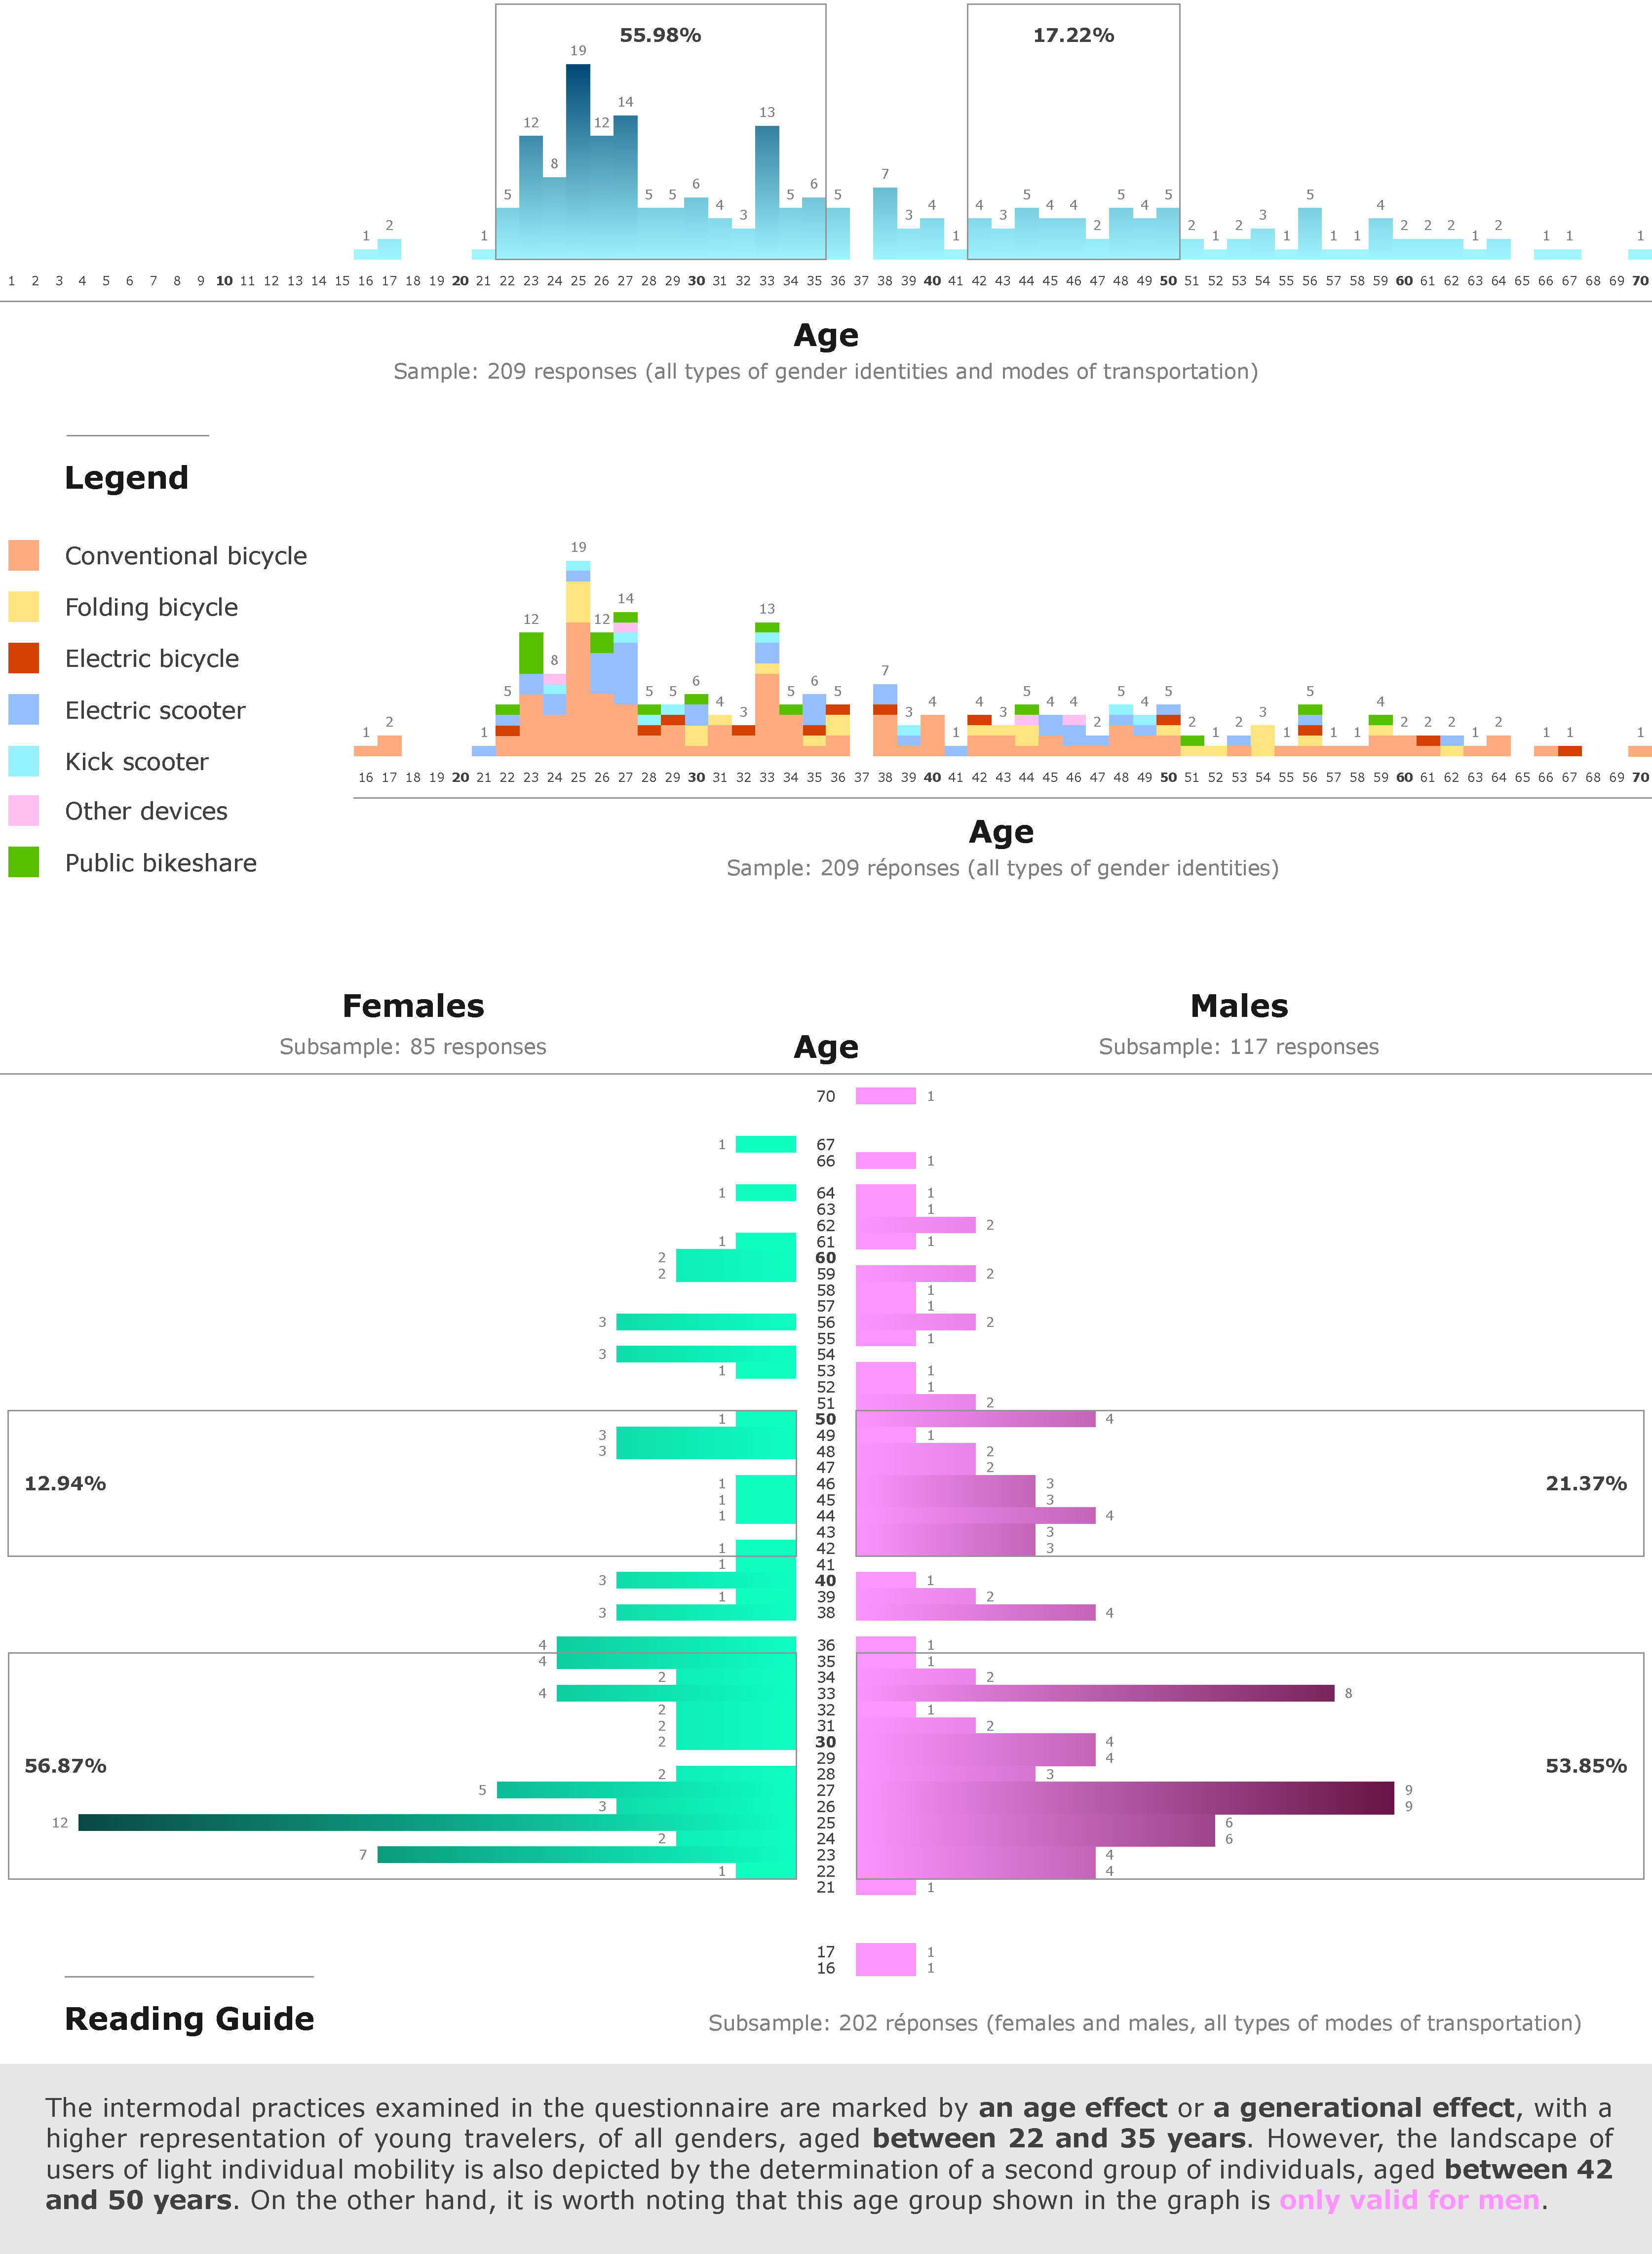
\includegraphics[width=1\columnwidth]{src/Figures/Chap-4/EN_Pyramide_age.pdf}}
        \vspace{5pt}
        \begin{flushright}\scriptsize{
        Author: \textcolor{blue}{Dylan Moinse (2024)}
        }\end{flushright}
    \end{figure}

    % Second pic
Overall, the age segment from 22 to 35 years comprises the majority of intermodal users of light individual mobility (56\%, 117 responses). However, it is worth noting a secondary peak among cycle travelers aged 42 to 50 years (17\%, 36 responses). This observation aligns with the segmentation of \acrshort{DESS} users in Germany, as described by \textcolor{blue}{\textcite[4]{degele_identifying_2018}}\index{Degele, Jutta|pagebf}\index{Gorr, Anna|pagebf}\index{Haas, Katja|pagebf}\index{Kormann, Dimitri|pagebf}\index{Krauss, Sascha|pagebf}\index{Lipinski, Paulina|pagebf}\index{Tenbih, Muhammet|pagebf}\index{Koppenhoefer, Christine|pagebf}\index{Fauser, Jan|pagebf}\index{Hertweck, Dieter|pagebf}, which shows a second peak of users aged 45 to 50 years who travel longer distances on average. It appears that the age groups corresponding to the youngest and the senior users are primarily underrepresented compared to rail travelers and the general French population demographics.%%Translated%%

    % Littérature technique
Referring to the age groups of travelers at train stations \textcolor{blue}{\autocite{sncf_repartition_2017}}\index{SNCF@\textsl{SNCF}|pagebf}, we can indeed observe that the least represented age groups within our subpopulation are those under 19 years old (1\% vs. 14\%), as well as those over 60 years old (6\% vs. 15\%), while the share of 20 to 39-year-olds is significant (64\% vs. 40\%). In comparison to the entire population \textcolor{blue}{\autocite{insee_age_2022}}\index{Insee@\textsl{Insee}|pagebf}, those under 19 years old (1\% vs. 23\%) and those over 65 years old (1\% vs. 22\%) remain marginalized. On the other hand, the most represented intervals are 20 to 34 years old (54\% vs. 17\%) and, to a lesser extent, 35 to 49 years old (25\% vs. 19\%).%%Translated%%

    % Littérature scientifique
In light of the knowledge accumulated in the scientific literature, we have shown that while bicycles and, even more so, micromobility are frequently favored by young users in monomodal use \textcolor{blue}{\autocites[3]{winters_who_2019}[6]{bielinski_electric_2020}[4, 11]{gioldasis_risk-taking_2021}[13]{speak_scooter_2023}[200]{yang_shared_2024}}\index{Bieliński, Tomasz|pagebf}\index{Ważna, Agnieszka|pagebf}\index{Yang, Wencui|pagebf}\index{Jafarzadehfadaki, Mostafa|pagebf}\index{Yan, Xiang|pagebf}\index{Zhao, Xilei|pagebf}\index{Jin, Xia|pagebf}\index{Frolich, Daniel|pagebf}\index{Sisiopiku, Virginia~P.|pagebf}\index{|pagebf}\index{Speak, Anna|pagebf}\index{Taratula-Lyons, Monique|pagebf}\index{Clayton, William|pagebf}\index{Shergold, Ian|pagebf}\index{Gioldasis, Christos|pagebf}\index{Christoforou, Zoi|pagebf}\index{Seidowsky, Régine|pagebf}\index{Winters, Meghan|pagebf}\index{Hosford, Kate|pagebf}\index{Javaheri, Sana|pagebf}, their use as a chaining solution is nuanced by a broadening of the demographic spectrum to include adults. Based on our questionnaire survey conducted in Provence-Alpes-Côte d'Azur, we were able to identify an overrepresentation of 25 to 34-year-olds among \acrshort{PeS} users, reaching 28\% compared to 16\% for the general passengers of \acrshort{TER}, with a second peak for 45 to 54-year-olds \textcolor{blue}{\autocite[183]{moinse_intermodal_2022}}\index{Moinse, Dylan|pagebf}\index{Goudeau, Matthieu|pagebf}\index{L'Hostis, Alain|pagebf}\index{Leysens, Thomas|pagebf}. Moreover, those under 17 years old and over 55 are less represented, while intermodal use of traditional bicycles is more frequent among 35 to 44-year-olds. The identification of a profile of cycle travelers predominantly in their thirties thus fits with various studies on the integration of light individual mobility \textcolor{blue}{\autocites[7]{rastogi_willingness_2010}[192]{sherwin_practices_2011}[321]{martin_evaluating_2014}[216]{lin_built_2018}[403]{weliwitiya_bicycle_2019}[184]{cao_e-scooter_2021}[8]{zhao_public_2022}}\index{Sherwin, Henrietta|pagebf}\index{Parkhurst, Graham|pagebf}\index{Robbins, Derek|pagebf}\index{Walker, Ian|pagebf}\index{Rastogi, Rajat|pagebf}\index{Krishna Rao,~K.~V.|pagebf}
\acrshort{PBS} \textcolor{blue}{\autocite[55]{zhao_bicycle-metro_2017}}\index{Zhao, Pengjun|pagebf}\index{Li, Shengxiao|pagebf}\index{Cao, Zhejing|pagebf}\index{Zhang, Xiaohu|pagebf}\index{Chua, Kelman|pagebf}\index{Yu, Honghai|pagebf}\index{Zhao, Jinhua|pagebf}\index{Weliwitiya, Hesara|pagebf}\index{Rose, Geoff|pagebf}\index{Johnson, Marilyn|pagebf}\index{Martin, Elliot~W.|pagebf}\index{Shaheen, Susan~A.|pagebf}\index{Zhao, Pengjun|pagebf}\index{Zhao, Pengjun|pagebf}\index{Takada, Kazuyuki|pagebf}\index{Li, Shengxiao|pagebf}\index{Yai, Tetsuo|pagebf}\index{Chen, Chi-Hao|pagebf}\index{Yuan, Dandan|pagebf}\index{Zhang, Yixue|pagebf}.%%Translated%%

    % Transition
This subsection highlighted the strong interest of young adults and adults, covering a wide spectrum from 25 to 50 years old, in light individual mobility coupled with the public transport network. However, the second demographic peak, detailed in the \hyperref[fig-chap4:pyramide-age]{Figure~\ref{fig-chap4:pyramide-age}} (page~\pageref{fig-chap4:pyramide-age}), is specifically observed among male users, where the age group of 42 to 50 years represents 21\% of respondents (25 responses), indicating that age-related disparities manifest differently depending on gender. This observed fact thus leads us to investigate the gender differences associated with these intermodal practices.%%Translated%%

    % 4.2.3.2.
    \needspace{1\baselineskip} % Space reservation
\subsubsection*{A Dual Effect of Age and Gender?
    \label{chap4:demographie-genre}
    }

% Introduction
In France, environmental convictions and lifestyle choices vary according to gender. Women generally show more ecological preferences across different social groups and geographical contexts \textcolor{blue}{\autocite[29]{pech_femmes_2021}}\index{Pech, Thierry|pagebf}\index{Witkowski, Didier|pagebf}. However, in terms of mobility, they are more reluctant to adopt modal shifts, such as reducing car usage or opting for cycling \textcolor{blue}{\autocite[25]{pech_femmes_2021}}\index{Pech, Thierry|pagebf}\index{Witkowski, Didier|pagebf}. Although women undertake a larger share of their daily trips by car, they maintain a lower carbon footprint than men, as their trips are generally 12\% to 17\% shorter due to the unequal distribution of family responsibilities. They also prefer walking and public transportation \textcolor{blue}{\autocite[6]{shaw_beyond_2020}}\index{Shaw, Caroline|pagebf}\index{Russell, Marie|pagebf}\index{Keall, Michael|pagebf}\index{MacBride-Stewart, Sara|pagebf}\index{Wild, Kirsty|pagebf}\index{Reeves, Dory|pagebf}\index{Bentley, Rebecca|pagebf}\index{Woodward, Alistair|pagebf}. The purpose of this subsection is to highlight the gender inequalities underlying multimodal practices and to analyze them in relation to various variables, in order to better understand the issues related to this social phenomenon. This knowledge production objective echoes \textsl{Objective 11.2} of the \textsl{2030 Agenda}, adopted in 2015 as part of the 17 \acrfull{SDGs}, which aims to promote more gender-equitable mobility systems \textcolor{blue}{\autocite{united_nations_transforming_2015}}\index{ONU@\textsl{ONU}|pagebf}. %%Translated%%

% Observation - general and modes
The observational study conducted in the Hauts-de-France region highlights the significant gender disparity in the multimodal use of light individual mobility, with this difference being even more pronounced than in the monomodal use of these same means. Thus, the combination of cycling and micromobility with public transport is particularly gendered, with an imbalance in favor of men. Female users account for only a quarter of the observed multimodal travelers (28\%, out of 1,035 observations), while they represent half of the counted railway travelers (49\%, out of 15,435 observations), thus highlighting this disparity (see \hyperref[fig-chap4:genre-age]{Figure~\ref{fig-chap4:genre-age}}, page~\pageref{fig-chap4:genre-age}). Moreover, significant variations emerge when considering the different vehicles involved. The most marked gender inequalities are observed for conventional bicycles (24\%, out of 329 observations), \acrshort{PeS} (25\%, out of 460 observations), and other types of micromobility such as skateboards or unicycles (26\%, out of 19 observations). Meanwhile, a more balanced gender distribution is observed in the case of folding bicycles (35\%, out of 123 observations) and mechanical scooters (49\%, out of 104 observations). %%Translated%%

% Figure Overview genre âge
\begin{figure}[h!]\vspace*{4pt}
    \caption{Sankey diagram representing the flows of multimodal cyclists, according to the surveyed station, vehicle type, age category, and gender.}
    \label{fig-chap4:genre-age}
    \centerline{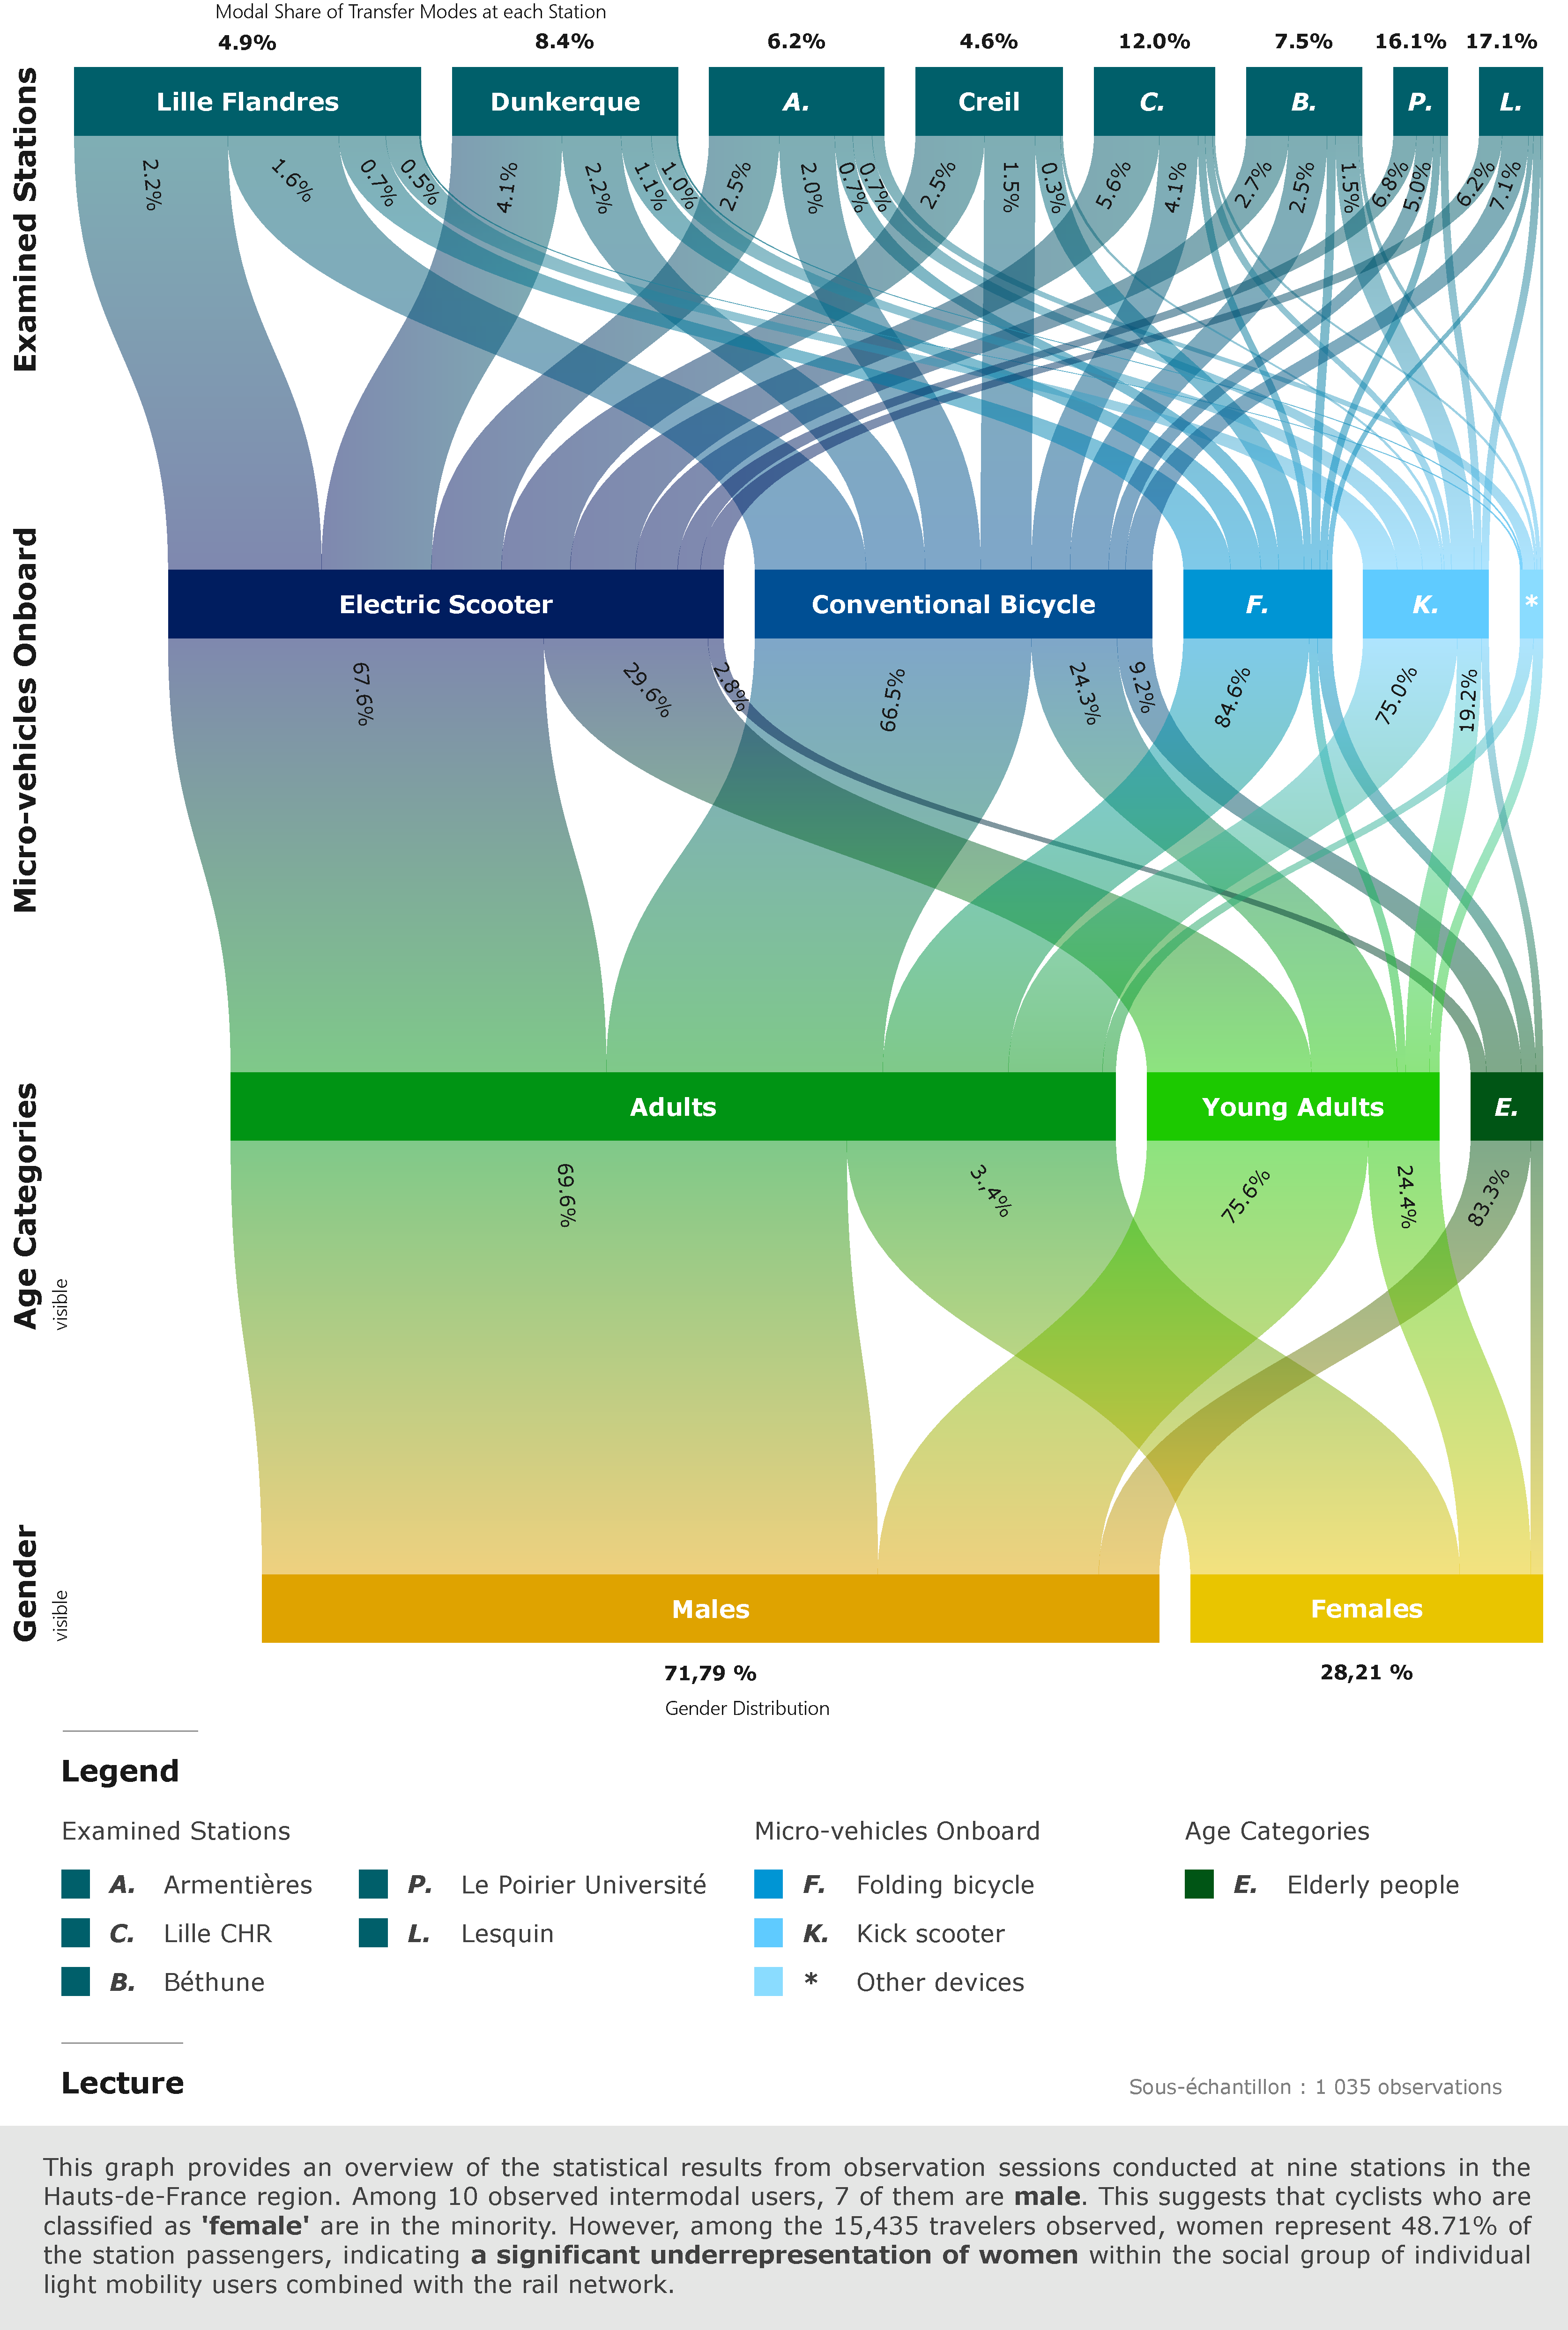
\includegraphics[width=1\columnwidth]{src/Figures/Chap-4/EN_Genre_Age.pdf}}
    \vspace{5pt}
    \begin{flushright}\scriptsize{
    Author: \textcolor{blue}{Dylan Moinse (2024)}
    }\end{flushright}
\end{figure}

% Questionnaire - general and modes
The questionnaire, whose result representativeness is limited—this technique relies on the voluntary participation of respondents, which may introduce selection bias—indicates that 43\% of intermodal cyclists are women (90 responses). This proportion varies from 40\% to 47\% for unicycles, skateboards, folding bicycles, mechanical scooters, conventional bicycles, and shared mobility (with 2, 10, 4, 47, and 7 responses, respectively). Gender parity is even exceeded for \acrshort{e-Bike}, where female users represent 69\% of participants (9 responses). \textsl{In contrast}, \acrshort{PeS} shows a considerable imbalance, with only 28\% female responses (11 responses). %%Translated%%

% Observation - cross-referenced with age
When jointly exploring the variables of gender and age, the analysis seems to indicate an exacerbation of gender inequalities with age progression, without being able to determine whether this is due to an age effect or a generational effect\footnote{~
    On one hand, the age effect refers to practices and preferences that naturally and socially change with an individual's age, regardless of their generation. Thus, it is possible that younger women show a more pronounced preference for the multimodal use of light individual mobility, or that men continue to use these modes of transportation longer than women, all other things being equal. On the other hand, the generational effect, or cohort effect, refers to the attitudes and values shared by individuals of the same generation. In this sense, women from the Alpha and Z generations (between 1997 and today) might be more inclined to use these vehicles than those from previous generations.
}. According to the established age categories, the imbalance in favor of male travelers using \acrshort{PeS} gradually strengthens: the male-to-female ratio is 2.7 among the \Commas{young adults}, increases to 3.1 among the \Commas{adults}, and reaches 12 among the \Commas{elderly}. %%Translated%%

% Literature - cycling
Echoing previous research, these descriptive statistics align with the admittedly limited body of scientific literature on the relationship between cycling use and gender in France \textcolor{blue}{\autocite[1]{gaudron-arlon_gender_2022}}\index{Gaudron-Arlon, Léa|pagebf}. Across all age groups, men cycle nearly three times more frequently than women, while women tend to walk more than men \textcolor{blue}{\autocite[2]{rossignol_femmes_2023}}\index{Rossignol, Françoise|pagebf}\index{Faucheux, Valérie|pagebf}\index{Revel-Fourcade, Armelle|pagebf}\index{Delli, Karima|pagebf}. In the context of both personal and shared cycling use, an analysis conducted by \textcolor{blue}{Matthieu} \textcolor{blue}{\textcite{adam_quart_2018}}\index{Adam, Matthieu|pagebf} on manual counts conducted by the Metropolis of Lyon highlights the clear predominance of male cyclists, who represent 59\% of the total. The report published by \textcolor{blue}{\textcite[27]{6t-bureau_de_recherche_etude_2018}}\index{Bureau de recherche 6t@\textsl{Bureau de recherche 6t}|pagebf}, focusing on the profile of \acrshort{DBS} users in Paris, corroborates this general observation, with men accounting for 68\%. The typology of users of Lyon's \acrshort{PBS} system, \textsl{Vélo'v}, carried out by \textcolor{blue}{\textcite[289]{vogel_bicycle_2014}}\index{Vogel, Marie|pagebf}\index{Hamon, Ronan|pagebf}\index{Lozenguez, Guillaume|pagebf}\index{Merchez, Luc|pagebf}\index{Abry, Patrice|pagebf}\index{Barnier, Julien|pagebf}\index{Borgnat, Pierre|pagebf}\index{Flandrin, Patrick|pagebf}\index{Mallon, Isabelle|pagebf}\index{Robardet, Céline|pagebf}, reveals an unequal gender distribution that varies across four identified categories: the \Commas{regular users} and the \Commas{frequent users} are predominantly male, while the categories related to \Commas{multimodal users} and \Commas{occasional users} show a more balanced gender distribution. However, in the context of our survey, the gender distribution of light individual mobility associated with the rail network does not appear to be linked to the frequency of use of these modal combinations. %%Translated%%

% Literature - scooter
A similar pattern emerges in the context of the recent rise of \acrshort{PeS}, with men representing around 60\% of users of this \acrshort{PMD} in France, as evidenced by the study of \textcolor{blue}{Cyprien} \textcolor{blue}{\textcite{richer_dossier_2021}}\index{Richer, Cyprien|pagebf} which consolidates approximately 40 certified mobility surveys by \acrfull{Cerema}. The prevalence of male users, ranging between 68\% and 75\%, is also found in the \acrshort{DESS} market. These gender inequalities in emerging mobility are observed not only in Paris \textcolor{blue}{\autocites[46]{apur_mobilites_2020}[14]{6t-bureau_de_recherche_comprendre_2019}[annexes]{bortoli_consequential_2020}}\index{Bureau de recherche 6t@\textsl{Bureau de recherche 6t}|pagebf}\index{Apur@\textsl{Apur}|pagebf}\index{Bortoli, Anne de|pagebf}\index{Christoforou, Zoi|pagebf}, but also in Lyon and Marseille \textcolor{blue}{\autocite[50]{6t-bureau_de_recherche_usages_2019}}\index{Bureau de recherche 6t@\textsl{Bureau de recherche 6t}|pagebf}. Similar to cycling, it has been found that the most frequent users of electric scooter services are predominantly men (68\%) compared to occasional users (58\%) in these three French metropolitan areas \textcolor{blue}{\autocite[65]{6t-bureau_de_recherche_usages_2019}}\index{Bureau de recherche 6t@\textsl{Bureau de recherche 6t}|pagebf}. In the context of the rail network in the Provence-Alpes-Côte d'Azur region, we identified a modal share of cycling and \acrshort{PeS} that is largely appropriated by men, with respective shares of 79\% and 83\%, while the overall distribution of railway travelers is gender-balanced and those connecting to stations by car are predominantly women \textcolor{blue}{\autocite[183]{moinse_intermodal_2022}}\index{Moinse, Dylan|pagebf}\index{Goudeau, Matthieu|pagebf}\index{L'Hostis, Alain|pagebf}\index{Leysens, Thomas|pagebf}. %%Translated%%

% Conclusion
This analysis has allowed for the definition of the socio-economic and demographic profile of multimodal users of light individual mobility, in order to examine these modal synergies as vectors of imbalances in terms of age and gender distribution. Within this subsection, focused on the categories of age and gender, as perceived and reported by travelers, three main trends emerge: (i) the statistical representation of a mobility practice predominantly engaged by adults, (ii) by men, while (iii) the gender distribution continues to become more unequal as the age of users increases. Thus, the combination of cycling and micromobility with public transport systems is not exclusive to younger people and is distinctly gendered. %%Translated%%

% Transition
At a time when light individual mobility, particularly the vehicles and services recently integrated into the mobility ecosystem, is predominantly adopted by male users, our empirical research has highlighted that the multimodal use of these vehicles, marked by a male overrepresentation, follows the same pattern. The use of motorized scooters, often favored in combination with trains, thus represents a new socio-cultural phenomenon in that the \acrshort{ePMD} is a gendered design object, just like bicycles \textcolor{blue}{\autocites[16]{clewlow_micromobility_2018}[17]{sayagh_adolescentes_2018}[2]{abord_dechatillon_velo_2021}}\index{Abord de Chatillon, Margot|pagebf}\index{Ortar, Nathalie|pagebf}\index{Sayagh, David|pagebf}\index{Sayagh, David|pagebf}\index{Clewlow, Regina|pagebf}. However, some of the literature suggests that the profile of cyclists tends to diversify when cycling practices are developed within territories. The more a territory is frequented by cyclists or the more cycle-friendly it is, the higher the number of women using bicycles would be \textcolor{blue}{\autocite{lardellier_cadres_2021}}\index{Lardellier, Rémi|pagebf}. This hypothesis invites us to question how to pave the way for more inclusive multimodal practices, particularly by considering the improvement of cycling infrastructure as a potential lever. We intend to further explore this hypothesis by examining the role of factors related to cycling practices, urban environment, and the perceived quality of public spaces on the gender distribution of these mobility practices. %%Translated%%

% ___________________________________________
% 4.3.
\newpage
\needspace{1\baselineskip} % Reserve space
\sectionheader{Gender Inequalities, Urban Planning as a Leverage for Action}
\section{Disparities in the Mobility Practices of Intermodal Cyclists and the Moderating Role of Urban Planning Action
    \label{section-chap4:cyclabilite-genre}
    }
%% Introduction
Based on recent scientific literature on the complex links between cycling and gender, this section aims to explore the interrelations between the modal share of cycling, the urban environment conducive to cycling, and female participation in this mode of transportation, within the framework of an empirical and comparative approach. In line with the recommendations made by \textcolor{blue}{\textcite[78]{goel_cycling_2022}}\index{Goel, Rahul|pagebf}\index{Goodman, Anna|pagebf}\index{Aldred, Rachel|pagebf}\index{Nakamura, Ryota|pagebf}\index{Tatah, Lambed|pagebf}\index{Garcia, Leandro Martin Totaro|pagebf}\index{Zapata-Diomedi, Belen|pagebf}\index{Sa, Thiago Herick de|pagebf}\index{Tiwari, Geetam|pagebf}\index{Nazelles, Audrey de|pagebf}\index{Tainio, Marko|pagebf}\index{Buehler, Ralph|pagebf}\index{Götschi, Thomas|pagebf}\index{Woodcock, James|pagebf}, this research seeks to examine the multiple parameters underlying these three variables by questioning the role of urban planning in different territories. However, it should be noted that this investigation aims to go beyond the reductive view of merely the geographic presence of cycling routes as an explanation for mobility and gender-related issues. To achieve this, we have chosen to embrace the concept of \Commas{bikeability}, focusing on cyclists' perceptions and experiences regarding the quality of the urban environment they frequent, in response to the main individual barriers hindering women's engagement with light individual mobility. %%Translated%%

%% Definition of bikeability
Just as \gls{walkability} is related to walking, \Commas{bikeability} refers to the degree of friendliness of a territory for cycling, promoting both safety, connectivity, comfort, and the pleasure of cycling. The evaluation of bikeability is expressed through an analysis of the level of service offered to cyclists, whether from an objective or subjective perspective, taking into account components such as accessibility \textcolor{blue}{\autocite[43]{lowry_assessment_2012}}\index{Lowry, Michael~B.|pagebf}\index{Callister, Daniel|pagebf}\index{Gresham, Maureen|pagebf}\index{Moore, Brandon|pagebf}. Despite its predominant role, and partly due to the difficulty of measuring it, the subjective assessment of bikeability is often overlooked, leading to the relegation of critical factors such as safety, comfort, and attractiveness related to cycling \textcolor{blue}{\autocite[173]{gan_associations_2021}}\index{Gan, Zuoxian|pagebf}\index{Yang, Min|pagebf}\index{Zeng, Qingcheng|pagebf}\index{Timmermans, Harry~J.~P.|pagebf}. Bikeability measurement can be undertaken at various scales, including through the evaluation of specific cycling routes \textcolor{blue}{\autocites[5]{hardinghaus_more_2021}[44]{lowry_assessment_2012}[454]{krenn_development_2015}[55]{mcneil_bikeability_2011}[5]{wysling_where_2022}[6]{schmid-querg_munich_2021}}\index{Hardinghaus, Michael|pagebf}\index{Nieland, Simon|pagebf}\index{Lehne, Marius|pagebf}\index{Weschke, Jan|pagebf}\index{Lowry, Michael~B.|pagebf}\index{Callister, Daniel|pagebf}\index{Gresham, Maureen|pagebf}\index{Moore, Brandon|pagebf}\index{Krenn, Patricia Jasmin|pagebf}\index{Oja, Pekka|pagebf}\index{Titze, Sylvia|pagebf}\index{McNeil, Nathan|pagebf}\index{Wysling, Laura|pagebf}\index{Purves, Ross~S.|pagebf}\index{Schmid-Querg, Jonas|pagebf}\index{Keler, Andreas|pagebf}\index{Grigoropoulos, Georgios|pagebf} or at a higher geographic level \textcolor{blue}{\autocites[4]{winters_bike_2016}[68]{gu_using_2018}[38]{nielsen_bikeability_2018}}\index{Winters, Meghan|pagebf}\index{Teschke, Kay|pagebf}\index{Brauer, Michael|pagebf}\index{Fuller, Daniel|pagebf}\index{Gu, Peiqin|pagebf}\index{Han, Zhiyuan|pagebf}\index{Cao, Zhejing|pagebf}\index{Chen, Yulin|pagebf}\index{Jiang, Yang|pagebf}\index{Nielsen, Thomas Alexander Sick|pagebf}\index{Skov-Petersen, Hans|pagebf}. %%Translated%%

% 4.3.1.
\needspace{1\baselineskip} % Reserve space
\subsection{Mobilization of Demographic Variables Integrated into the Mixed Methods Implemented
    \label{chap4:materiau-empirique-genre}
    }

%% Introduction
This subsection details the various databases used in the development of a statistical regression model. The analysis is designed to study the influence of factors related to the urban environment, both measured and perceived, on the differentiated practices of cycling and micromobility according to gender. The identified dependent variables include the rate of female participation in exclusive bicycle use as well as the gendered use of light individual mobility in an intermodal context. The independent variables, on the other hand, include factors such as the modal share of cycling, population density, the cycling network, and the bikeability score as perceived by users. This data structuring underlying the model aims to provide relevant insights into gender dynamics in urban space. %%Translated%%

%% Definition of bikeability
In this context, the framework built by the independent indicators focuses on several dimensions: the modal share of cycling, population density, objective bikeability, and perceived bikeability. For the latter two dimensions, we integrate aspects related to the urban environment into the measured bikeability, notably the proportion of cycling infrastructure and the proportion of 30 km/h zones relative to the road network in each municipality. Individual and perceived bikeability, on the other hand, is assessed at aggregated levels for each municipality, based on the responses collected from the analyzed questionnaire, which includes 5 dimensions and 26 underlying thematic questions, ranging from \(Q_{14}\) to \(Q_{39}\) (see \hyperref[annexes:structure-questionnaire-fub-questions]{Appendix~\ref{annexes:structure-questionnaire-fub-questions}}, page~\pageref{annexes:structure-questionnaire-fub-questions}). This method allows us to propose an analysis based on the mobility system (use of light individual mobility), the urban system (population density), the design of public spaces (cycling infrastructure), and the individual experience of transport modes in the studied cities. %%Translated%%

% 4.3.1.1.
\needspace{1\baselineskip} % Reserve space
\subsubsection*{Secondary Analysis of the \textsl{MOBPro} File from the Population Census
    \label{source-mobpro}
    }

%% \textsl{MOBPro} 2019 Description 1
This empirical research is based, firstly, on the data from the 2019 periodic population census conducted by \textcolor{blue}{\textcite{insee_documentation_2023}}\index{Insee@\textsl{Insee}|pagebf}, which is carried out every four years. More specifically, the data examined comes from the file titled \Commas{\textsl{Mobilités Professionnelles}} (\textsl{MOBPro}), which focuses exclusively on the study of daily travel made by individuals living in France. It should be noted that, in response to this survey, households had the option to provide individual responses either electronically or by mail. The database from this census provides an accurate representation of travel between home and the workplace, based on a comprehensive sample that includes active individuals aged 15 and over, residing in both metropolitan France and the \acrfull{DROM-COM}\footnote{~
    The \acrfull{DROM} have both departmental and regional status, and are integrated into the French Republic just like the previously mentioned metropolitan regions. The \acrshort{DROM} are part of the French overseas territories \acrshort{DROM-COM}, along with the \acrfull{COM} which have a different status and greater autonomy from metropolitan France.
}, excluding Mayotte. %%Translated%%

%% \textsl{MOBPro} 2019 Description 2
The questions formulated and used within the \textsl{MOBPro} dataset mainly focus on two variables: the workplace locations at the municipal level (\(Q^{Insee}_{20}\)) and the primary mode of transportation (\(Q^{Insee}_{22}\)). Each individual is anonymized and is described by their commuting patterns, socio-demographic characteristics, as well as residential and professional locations at the municipal scale. Taking into account the weighting factors specific to each individual allows these data to be used to form a representative sample when there are at least 200 responses per municipality \textcolor{blue}{\autocite{insee_documentation_2023}}\index{Insee@\textsl{Insee}|pagebf}. Furthermore, it should be noted that a modification was made to the questionnaire starting in 2015, which resulted in a clear distinction between \Commas{bicycles} and \Commas{motorized two-wheeled vehicles} \textcolor{blue}{\autocite{razemon_pour_2013}}\index{Razemon, Olivier|pagebf}. This change was implemented in question \(Q^{Insee}_{22}\), which now explicitly includes \Commas{bicycles (including electric bicycles)}. %%Translated%%

%% \textsl{MOBPro} 2019 Sampling 1
The 2019 \textsl{MOBPro} database, encompassing a total of 7,932,895 individuals, contains a set of filtered variables, including individual weight (\Commas{\(IPONDI\)}), the primary mode of transportation used for home-to-work trips (\Commas{\(TRANS\)}), the place of residence (\Commas{\(COMMUNE\)}), and gender (\Commas{\(SEXE\)}). The first inclusion criterion, applied using a series of \textsl{Python} codes, focuses on the primary mode of transportation associated with cycling (\Commas{\(TRANS~=~3\)}), thus excluding other mobility modalities, as carried out by \textcolor{blue}{\textcite[7]{raux_does_2021}}\index{Raux, Charles|pagebf}\index{Lamatkhanova, Ayana|pagebf}\index{Grassot, Lény|pagebf}. This approach excludes intermodal trips where cycling is used as a secondary mode of transport, due to the statistical parameters applied\footnote{~
    In most mobility surveys in France, the hierarchy of transportation modes is generally established based on the primary mode used for intermodal trips. The \textsl{Enquêtes Mobilité Certifiées \acrshort{Cerema}} adhere to the convention established by \textcolor{blue}{\textcite[32]{cerema_enquetes_2020}} which gives priority to so-called \Commas{structuring} modes.
} \textcolor{blue}{\autocite[32]{cerema_enquetes_2020}}. This procedure resulted in a sub-sample of 409,326 individuals, consisting of 253,464 male cyclists and 155,862 female cyclists. The descriptive statistical analysis reveals that only 1.5\% of women reported using a bicycle for their home-to-work trips, compared to 3.7\% of men. %%Translated%%

%% \textsl{MOBPro} 2019 Sampling 2
The second phase of exclusion applied to the \textsl{MOBPro} database involved aggregating commuters within similar municipalities \textcolor{blue}{\autocite{insee_documentation_2023}}\index{Insee@\textsl{Insee}|pagebf}, following the approach adopted by \textcolor{blue}{\textcite[259]{papaix_potential_2022}}\index{Papaix, Claire|pagebf}\index{Dupont-Kieffer, Ariane|pagebf}\index{Palmier, Patrick|pagebf}. Responses that were grouped and did not meet the significance threshold of 200 cyclists were excluded in order to maintain a representative diversity of territories\footnote{~
    In the documentation of the \textcolor{blue}{\textcite{insee_documentation_2023}}, regarding the \Commas{MOBPro} file, it is stated that \Commas{sample sizes greater than 500 can normally be used with confidence. Sample sizes smaller than 200 should be handled with caution as, due to the sampling imprecision, they may not be significant. Thus, comparisons between small territories should be avoided. For areas with fewer than 2,000 inhabitants, it is recommended not to use data from supplementary analysis.}.
}. Following the implementation of this selective filter, among the 10,520 municipalities with at least one cyclist in the database, 144 municipalities were retained, comprising 128,492 cyclists, of whom 76,773 were men and 51,719 were women. Of the 144 selected municipalities, 65 are central cities, while the remaining 79 are peripheral municipalities. %%Translated%%

% 4.3.1.2.
\needspace{1\baselineskip} % Reserve space
\subsubsection*{Mobilization of Quantitative Observation
    \label{chap4:variables-age-genre-observation-quantitative}
    }

%% Justification of Quantitative Observation
In addition to the secondary analysis of the aforementioned databases, this empirical research relies on the implementation of quantitative observation in order to capture the demographic profiles of micromobility users within our case study, focused on the Hauts-de-France region. Since these secondary data are limited to bicycle use, it seems essential to include modes of transportation associated with emerging micromobility, such as \acrshort{PeS}. This data collection method also aims to obtain a representative sample of multimodal travelers, thus combining light individual mobility with public transportation networks. %%Translated%%

% 4.3.1.3.
\needspace{1\baselineskip} % Reserve space
\subsubsection*{Use of the \textsl{Cyclable Cities Barometer}
    \label{chap4:source-barometre-fub}
    }

%% FUB Barometer Description
The second data source used to collect attributes related to the cycling environment is based on the exploitation of the biennial questionnaire from the \Commas{\textsl{Cyclable Cities Barometer}} of 2021, developed by \textcolor{blue}{\textcite{fub_barometre_2021}}\index{FUB@\textsl{FUB}|pagebf} in France. Deployed since 2017, this barometer aims to assess the bikeability of French municipalities through the compilation of cyclists' feedback regarding the quality of cycling infrastructure, implemented cycling policies, and the overall experience of users. The objective of this online questionnaire is to understand the general \gls{perception} of cyclists in France and to rank municipalities based on their perceived bike-friendliness. Today, this barometer serves as a reference point for local authorities, associations, researchers, and the general public. This subsection dedicated to the study of gender in mobility incorporates the concept of \Commas{subjective bikeability} in its analysis, recognizing that safety is both a collective and individual dimension, shaped by cyclists' experiences \textcolor{blue}{\autocite[57]{garrard_promoting_2008}}\index{Garrard, Jan|pagebf}\index{Rose, Geoffrey|pagebf}\index{Lo, Sing Kai|pagebf}\index{Rose, Geoffrey|pagebf}\index{Lo, Sing Kai|pagebf}. Furthermore, in line with the observations of \textcolor{blue}{\textcite[303]{ma_peoples_2017}}\index{Ma, Liang|pagebf}\index{Dill, Jennifer|pagebf}, a gap has been observed between the objective environment and the perceived environment in terms of bike-friendliness, particularly regarding its utilitarian use and partly attributed to the varying tolerance of risk depending on gender. %%Translated%%

%% FUB Barometer Questions
The questionnaire related to bikeability was administered online, providing both cyclists and non-cyclists the opportunity to evaluate their experiences or perceptions and to express their opinions regarding conditions related to cycling. The evaluations were conducted on a rating scale ranging from 1—indicating a \textsl{very unsatisfactory} level of satisfaction—to 6—\textsl{very satisfactory}. The various assessments made by participants were then compared to give an overall evaluation of the bikeability of each concerned municipality (see \hyperref[annexes:structure-questionnaire-fub-questions]{Appendix~\ref{annexes:structure-questionnaire-fub-questions}}, page~\pageref{annexes:structure-questionnaire-fub-questions}). This publicly accessible questionnaire consists of a set of twenty-six questions related to the respondents' cycling experiences, organized into five distinct themes: (i) \Commas{overall feeling}, (ii) \Commas{safety}, (iii) \Commas{comfort}, (iv) \Commas{city efforts}, and (v) \Commas{services and parking}. Using an overall score, municipalities are assigned a position on a scale from \(A+\) (scoring higher than 4.6 out of 6) to \(G\) (scoring below 2.3 out of 6), corresponding to a rating of the \Commas{cycling climate} of the territories, ranging from \Commas{excellent conditions} to \Commas{very unfavorable conditions} \textcolor{blue}{\autocite{fub_barometre_2021}}\index{FUB@\textsl{FUB}|pagebf}. It should be noted that the average score obtained by each French municipality reaches a general bikeability level of 2.98 out of 6 \textcolor{blue}{\autocite[17]{vermeulen_barometre_2022}}\index{Vermeulen, Thibault|pagebf}\index{Kaouane, Carole|pagebf}. A detailed statement of each question included in the rating for this barometer is presented in the \hyperref[annexes:structure-questionnaire-fub-tableau]{Appendix~\ref{annexes:structure-questionnaire-fub-tableau}} (page~\pageref{annexes:structure-questionnaire-fub-tableau}). %%Translated%%

    % Tableau Liste communes
% Table List of Municipalities
%%Rédigé%%
    \begin{table}[h!]
    \centering
    \renewcommand{\arraystretch}{1.5}
    \resizebox{\columnwidth}{!}{
    \begin{tabular}{p{0.34\columnwidth}p{0.56\columnwidth}p{0.1\columnwidth}}
        %\hline
    \rule{0pt}{15pt} \small{\textcolor{blue}{{\textbf{Region}}}} & \small{\textcolor{blue}{{\textbf{Central Cities}}}} & \small{\textcolor{blue}{{\textbf{Number of Cities}}}}\\
        \hline
\multirow{1.5}{*}{\small{Auvergne-Rhône-Alpes}} & \small{Annecy, Chambéry, Clermont-Ferrand, Grenoble, Lyon, Saint-Étienne, and Valence} & \multirow{1.5}{*}{\small{7}}\\
\small{Bourgogne-Franche-Comté} & \small{Besançon and Dijon} & \small{2}\\
\small{Bretagne} & \small{Brest, Lorient, Rennes, and Saint-Nazaire} & \small{4}\\
\small{Centre-Val de Loire} & \small{Orléans and Tours} & \small{2}\\
\multirow{1.5}{*}{\small{Grand Est}} & \small{Metz, Mulhouse, Nancy, Reims, Strasbourg, and Troyes} & \multirow{1.5}{*}{\small{6}}\\
\multirow{1.5}{*}{\small{Hauts-de-France}} & \small{Amiens, Arras, Beauvais, Douai, Dunkerque, Lille, and Valenciennes} & \multirow{1.5}{*}{\small{7}}\\
\small{Île-de-France} & \small{Paris} & \small{1}\\
\small{Normandie} & \small{Caen, Le Havre, and Rouen} & \small{3}\\
\multirow{1.5}{*}{\small{Nouvelle-Aquitaine}} & \small{Angoulême, Bayonne, Bordeaux, La Rochelle, Limoges, and Poitiers} & \multirow{1.5}{*}{\small{6}}\\
\small{Occitanie} & \small{Montpellier, Nîmes, Perpignan, and Toulouse} & \small{4}\\
\small{Pays de la Loire} & \small{Angers, Le Mans, and Nantes} & \small{3}\\
\multirow{1.5}{*}{\small{Provence-Alpes-Côte d'Azur}} & \small{Aix-en-Provence, Avignon, Marseille, Nice, and Toulon} & \multirow{1.5}{*}{\small{5}}\\
\small{La Réunion} & \small{Saint-Denis, Saint-Paul, and Saint-Pierre} & \small{3}\\
        \hline
        \end{tabular}}
    \caption{List of the 53 French municipalities examined in the study on bikeability in relation to gendered bicycle and micromobility practices.}
    \label{table-chap4:communes-fub-insee}
        \vspace{5pt}
        \begin{flushleft}\scriptsize
        \textcolor{blue}{Reading Guide:} This table lists the 53 French municipalities distributed across 13 regions, including large cities and medium-sized towns, to study the links between their bikeability and gendered bicycle practices.
        \end{flushleft}
        \begin{flushright}\scriptsize{
        Datasets: \textsl{MOBPro} \textcolor{blue}{\autocite{insee_documentation_2023}} and \textsl{Baromètre des Villes Cyclables} \textcolor{blue}{\autocite{fub_barometre_2021}}
        \\
        Author: \textcolor{blue}{Dylan Moinse (2023)}
        }\end{flushright}
        \end{table}%%Rédigé%%

%% FUB Barometer Sampling
The survey conducted by \textcolor{blue}{\textcite{fub_barometre_2021}}\index{FUB@\textsl{FUB}|pagebf} took place from September 14 to November 30, 2021, gathering a total of 277,384 responses, of which 250,228 came from cyclists. Only municipalities that received at least 50 responses from cyclists were included in the barometer ranking. Thus, 1,625 municipalities are represented in this third edition, divided into various categories: 38 large cities, 218 medium-sized cities, 353 small municipalities, 292 villages, 719 suburban municipalities, and 5 islands \textcolor{blue}{\autocite[7]{vermeulen_barometre_2022}}\index{Vermeulen, Thibault|pagebf}\index{Kaouane, Carole|pagebf}. Among the cyclists who participated in the 2021 \textsl{Cyclable Cities Barometer} survey, 46\% identified as women, excluding those respondents who did not specify their gender identity. This response rate reflects a four-point increase in female participation compared to the 2019 edition \textcolor{blue}{\autocite[10]{vermeulen_barometre_2022}}\index{Vermeulen, Thibault|pagebf}\index{Kaouane, Carole|pagebf}. By performing an attribute join between the 144 cities with more than 200 cyclists who responded to the \textsl{MOBPro} database and the cities included in the \textsl{Cyclable Cities Barometer} that received at least 100 individual ratings, the sampling process retained a sample of 64 French municipalities. We then chose to keep only the central cities of French urban areas in the sample, resulting in a final sample of 53 cities. The list of these 53 municipalities, classified by their respective regions, is presented in the \hyperref[table-chap4:communes-fub-insee]{Table~\ref{table-chap4:communes-fub-insee}} (page~\pageref{table-chap4:communes-fub-insee}). %%Translated%%

% 4.3.1.4.
\needspace{1\baselineskip} % Reserve space
\subsubsection*{Sources of Cartographic Data
    \label{chap4:source-cartographique}
    }

%% OpenStreetMap
Through the sampling based on these two databases, we were able to characterize the fifty-three French urban areas in terms of the modal share and gendered use of bicycles, as well as the subjective bikeability of the territory. Subsequently, in order to quantify the infrastructural dimension, these variables were significantly enriched with secondary data drawn from \textcolor{blue}{\textcite{openstreetmap_openstreetmap_2023}}\index{OpenStreetMap@\textsl{OpenStreetMap}|pagebf} and extracted on August 21, 2023. These cartographic data provide access to geographical information concerning cycling infrastructure in a given city. Moreover, this research on mobility and gender integrated data from the \Commas{\textsl{National Database of Cycling Infrastructure}} created by \textcolor{blue}{\textcite{velo__territoires_atlas_2023}}\index{Vélo \& Territoires@\textsl{Vélo \& Territoires}|pagebf} and the \Commas{\textsl{Municipal Density Grid}} from \textcolor{blue}{\textcite{insee_grille_2021}}\index{Insee@\textsl{Insee}|pagebf}. The contribution of this cartographic data allows the evaluation of the objective bikeability of each municipality based on the proportion of cycling infrastructure in the road network and the population density in the compared municipalities. %%Translated%%

% 4.3.2.
\needspace{1\baselineskip} % Reserve space
\subsection{Development of a Statistical Analysis Framework
    \label{chap4:methodologie-modele-ols}
    }

%% Introduction
The regression model implemented in this section aims to investigate the influence of factors on the use of bicycles and micromobility, specific to each gender, in both monomodal and intermodal contexts. The \hyperref[fig-chap4:schema-methodologie-ols]{diagram~\ref{fig-chap4:schema-methodologie-ols}} (page~\pageref{fig-chap4:schema-methodologie-ols}) presents the methodological framework used to carry out an \acrfull{OLS}, or ordinary least squares regression, including the preliminary steps required to evaluate the model's hypotheses and its validation. The steps and equations used have been detailed in the \hyperref[annexes:methodologie-ols-etapes]{Appendix~\ref{annexes:methodologie-ols-etapes}} (page~\pageref{annexes:methodologie-ols-etapes}). %%Translated%%

%% Figure OLS Methodological Diagram
\begin{figure}[h!]\vspace*{4pt}
    \caption{Diagram of the ordinary least squares modeling process examining the interactions between bikeability and the gendered use of bicycles and micromobility.}
    \label{fig-chap4:schema-methodologie-ols}
    \centerline{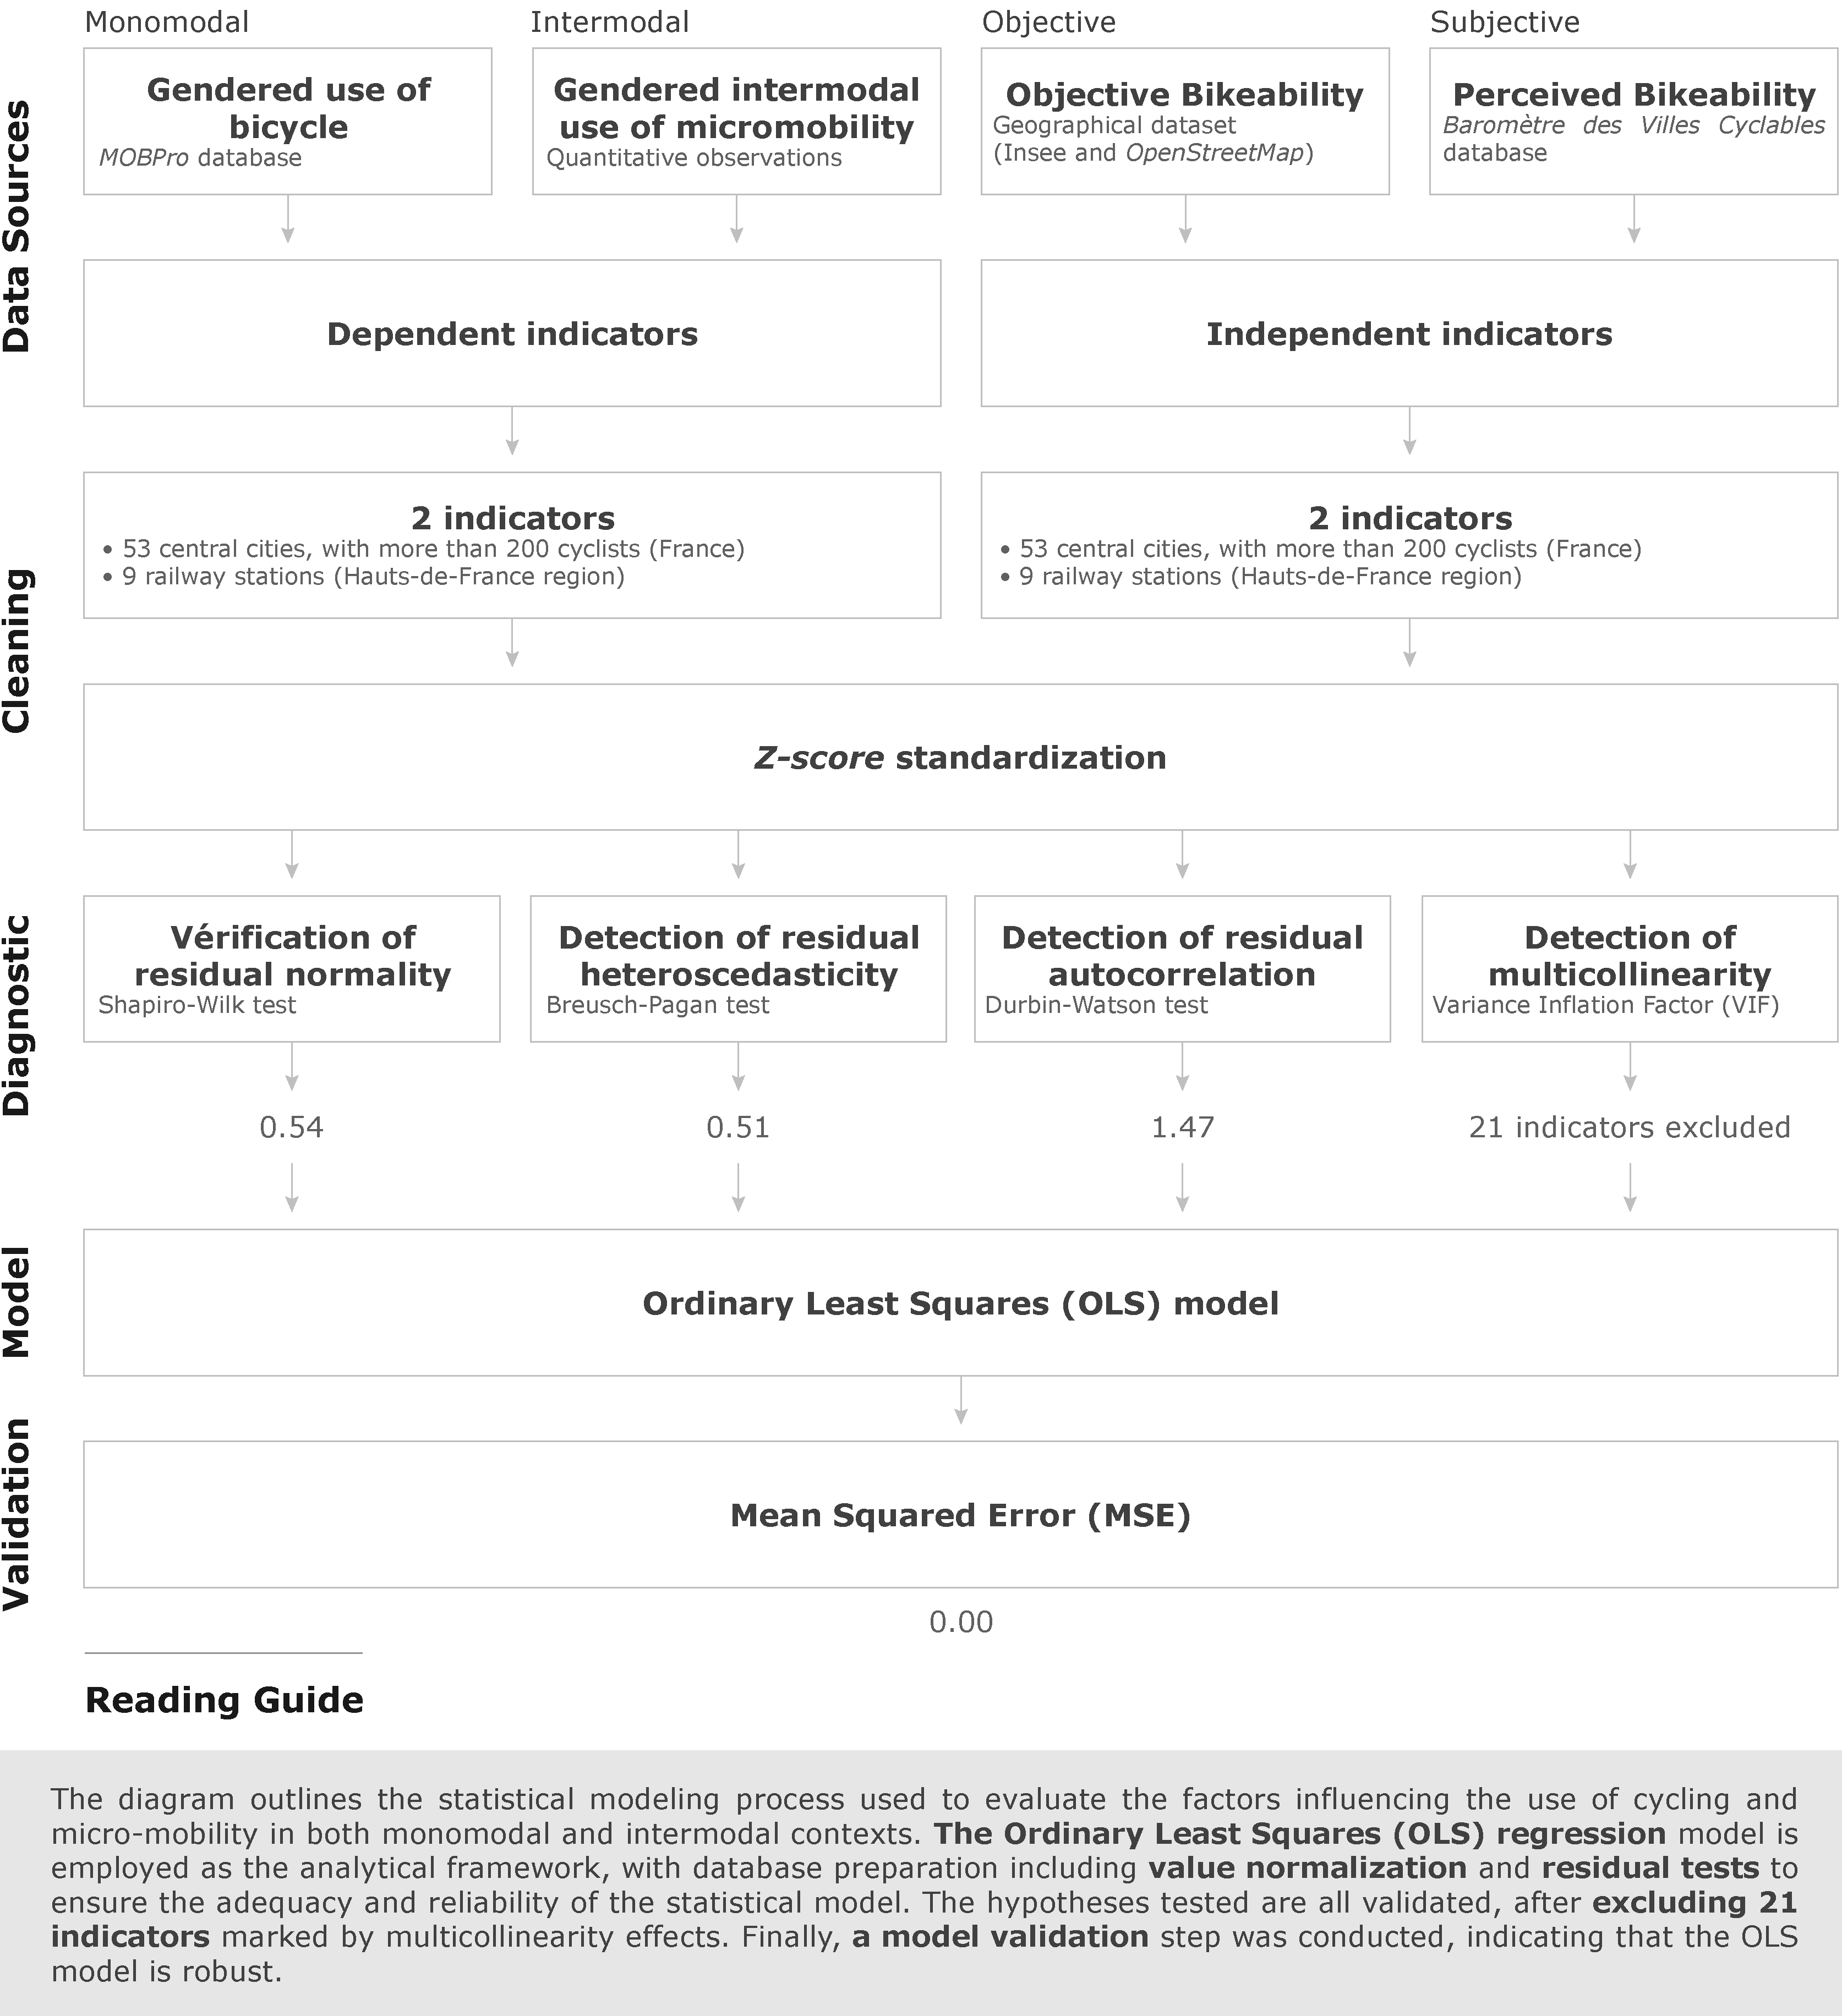
\includegraphics[width=1\columnwidth]{src/Figures/Chap-4/EN_Schema_Methodologie_OLS.pdf}}
    \vspace{5pt}
    \begin{flushright}\scriptsize{
    Author: \textcolor{blue}{Dylan Moinse (2023)}
    }\end{flushright}
\end{figure}

%% OLS Model
The secondary analysis is based on two databases used to support our approach, namely the 2019 \textsl{MOBPro} database \textcolor{blue}{\autocite{insee_documentation_2023}}\index{Insee@\textsl{Insee}|pagebf} and the 2021 \textsl{Cyclable Cities Barometer} \textcolor{blue}{\autocite{fub_barometre_2021}}\index{FUB@\textsl{FUB}|pagebf}. This analysis also relies on the quantitative observation from our case study. The use of descriptive statistical methods combined with the development of a linear regression model constitutes the methodological approach employed in this subsection. In this context, \acrshort{OLS} regression was chosen for this research due to its robustness in estimating linear relationships between a dependent variable and several independent variables. The main objective of this research is to clarify how various factors influence the modal share of women using bicycles in different French cities. \acrshort{OLS} regression is particularly suited for this objective as it allows for unbiased and efficient estimation of regression coefficients, provided that certain assumptions are met. Moreover, it enables quantifying the impact of each explanatory variable while controlling for the effects of other variables in the model. Furthermore, the selection of this statistical method is inspired by previous academic research that employed similar techniques to explore the relationships between the socio-demographic characteristics of a population and its urban environment. This research is thus inspired by the investigation conducted by \textcolor{blue}{\textcite[64]{goel_cycling_2022}}\index{Goel, Rahul|pagebf}\index{Goodman, Anna|pagebf}\index{Aldred, Rachel|pagebf}\index{Nakamura, Ryota|pagebf}\index{Tatah, Lambed|pagebf}\index{Garcia, Leandro Martin Totaro|pagebf}\index{Zapata-Diomedi, Belen|pagebf}\index{Sa, Thiago Herick de|pagebf}\index{Tiwari, Geetam|pagebf}\index{Nazelles, Audrey de|pagebf}\index{Tainio, Marko|pagebf}\index{Buehler, Ralph|pagebf}\index{Götschi, Thomas|pagebf}\index{Woodcock, James|pagebf}, which used these correlations to identify the links between the socio-demographic characteristics of cyclists and the urban environment in seventeen different countries. %%Translated%%

%% Formula
In this statistical analysis, the dependent variable is the proportion of light individual mobility use by women, while all other indicators analyzed serve as independent variables. These indicators include the overall modal share of cycling, the rate of cycling infrastructure and 30 km/h zones compared to the road network, population density, as well as the sub-questions establishing the perceived bikeability score derived from the questionnaire, totaling the integration of 35 variables. The multivariate analysis was conducted using \acrshort{OLS} regression, allowing us to assess the combined effect of all independent variables on the dependent variable. The \hyperref[equation:ols]{regression formula~\ref{equation:ols}} (page~\pageref{equation:ols}) is applied to estimate the linear relationship between the dependent variables and all the independent variables\footnote{~
    In this context, the intercept represents the estimated value of the dependent variable \(Y\) (the gendered modal share of cycling) when all the independent variables \(X_i\) are equal to zero. This is the point where the estimated regression line intersects the y-axis. In other words, \(\hat{\beta}_0\) is the value of \(Y\) predicted by the model when the contributions of all independent variables are null. This provides a baseline for interpreting the effects of independent indicators on the gendered modal share of cycling.
} \textcolor{blue}{\autocite{strang_introduction_1986}}\index{Strang, Gilbert|pagebf}. However, modeling requires verifying that the assumptions of linearity, independence, homoscedasticity, and normality of errors are met. The next step is to test the model's assumptions to refine and improve the statistical model. %%Translated%%

%% OLS Equation
\begin{equation}
\label{equation:ols}
\begin{aligned}
Y = \hat{\beta}_0 + \sum_{i=1}^{n} \hat{\beta}_i X_i + \epsilon
\end{aligned}
\end{equation}
\begin{align*}
    &\text{where:} \\
    &Y \text{ represents the gendered modal share of cycling;} \\
    &\hat{\beta}_0 \text{ is the estimated intercept;} \\
    &\hat{\beta}_i \text{ is the estimated coefficient for each independent variable } i\text{;}\\
    &X_i \text{ represents the independent variables } i\text{;}\\
    &\epsilon \text{ is the error term;} \\
    &n \text{ is the total number of independent indicators.}
\end{align*} %%Translated%%

% 4.3.2.1.
\needspace{1\baselineskip} % Reserve space
\subsubsection*{Verification of the Model Assumptions
    \label{chap4:methodologie-hypotheses}
    }

%% Z-score
The first step in cleaning merged databases is to standardize the explanatory variables before proceeding with the specific steps of the regression model. When characteristics have different scales, it can be difficult to directly compare the regression coefficients. Standardization places all variables on the same scale, making it easier to compare the relative effects of the explanatory variables. Before training the model, the data distribution is adjusted to have a mean of 0 and a standard deviation of 1 through normalization by the \(Z\)-score. This method, commonly used in linear regression \textcolor{blue}{\autocite{pearson_lines_1901}}\index{Pearson, Karl|pagebf}, is less sensitive to outliers because it relies on the standard deviation ($\sigma$), which is influenced but not dominated by extreme values. %%Translated%%

%% Shapiro-Wilk Test
Subsequently, the regression assumptions, including linearity, independence of errors, homoscedasticity, and normality of residuals, can be verified and diagnosed using statistical tests, ensuring the robustness and reliability of the statistical results. The normality of the residuals was tested using two methods: (i) normality and (ii) homoscedasticity of the residuals. It is important to first test the normality assumption for the significance tests of the regression coefficients. If the residuals do not follow a normal distribution, confidence intervals and hypothesis tests may be invalid. The Shapiro-Wilk test (\(W\)) gave a \(p\)-value of 0.542, indicating that the residuals follow a normal distribution \textcolor{blue}{\autocite{shapiro_analysis_1965}}\index{Shapiro, Samuel Sanfort|pagebf}\index{Wilk, Martin|pagebf}. %%Translated%%

%% Breusch-Pagan Test
Homoscedasticity implies that the errors have a constant variance across all levels of the dependent variable. This assumption is crucial because heteroscedasticity, meaning the non-constant variance of residuals, can lead to inefficient estimates of regression coefficients and biased standard errors, thereby affecting significance tests. The Breusch-Pagan Lagrange multiplier test statistic for homoscedasticity produced a \(p\)-value of 0.514, indicating that the homoscedasticity assumption cannot be rejected \textcolor{blue}{\autocite{breusch_simple_1979}}\index{Breusch, Trevor|pagebf}\index{Pagan, Adrian|pagebf}. %%Translated%%

%% Residual Autocorrelation
Residual autocorrelation occurs when the regression errors are correlated with each other, thus violating the assumption of independence of errors. This can lead to biased estimates of the coefficients and incorrect standard errors. To detect autocorrelation, we used the Durbin-Watson test. The Durbin-Watson statistic (\(DW\)) ranges from 0 to 4, with a value close to 2 indicating the absence of autocorrelation \textcolor{blue}{\autocite{durbin_testing_1950}}\index{Durbin, James|pagebf}\index{Watson, Geoffrey|pagebf}. Values close to 0 suggest positive autocorrelation, while values close to 4 indicate negative autocorrelation. Our test produced a statistic of 1.466, indicating the absence of significant autocorrelation. %%Translated%%

%% VIF
Next, we conducted an analysis using the variance inflation factor (\(VIF\)) for each variable to examine the multicollinearity of the model. Including multiple independent variables in the model allows us to see how each affects the dependent variable while controlling for the effects of the others. Multivariate analysis can reveal interactions between variables and highlight multicollinearity issues, where the explanatory variables are highly correlated with each other. High multicollinearity increases the standard errors of the coefficients, making them less reliable and complicating the determination of each predictor's effect. Our goal is to identify and address variables that lead to unstable coefficient estimates. The \(VIF\) values indicate the degree of multicollinearity among the independent variables \textcolor{blue}{\autocites{akinwande_variance_2015}{tamura_mixed_2019}}\index{Akinwande, Michael Olusegun|pagebf}\index{Dikko, Hussaini Garba|pagebf}\index{Samson, Agboola|pagebf}\index{Tamura, Ryuta|pagebf}\index{Kobayashi, Ken|pagebf}\index{Takano, Yuichi|pagebf}\index{Miyashiro, Ryuhei|pagebf}\index{Nakata, Kazuhide|pagebf}\index{Matsui, Tomomi|pagebf}. %%Translated%%

%% Autocorrelation
\hyperref[fig-chap4:matrice-autocorrelation]{Figure~\ref{fig-chap4:matrice-autocorrelation}} (page~\pageref{fig-chap4:matrice-autocorrelation}) presents the correlation matrix encompassing all the indicators included in the regression model. This matrix, which shows the relationships between the explanatory indicators, is an essential tool for understanding the interactions between these variables, thus helping to identify potential multicollinearity issues and discerning how different factors jointly influence the gendered modal share of cycling. This approach ensures unbiased and efficient estimates of the regression coefficients. %%Translated%%

%% Figure Correlation Matrix
\begin{figure}[h!]\vspace*{4pt}
    \caption{Correlation matrix of the indicators included in the regression model.}
    \label{fig-chap4:matrice-autocorrelation}
    \centerline{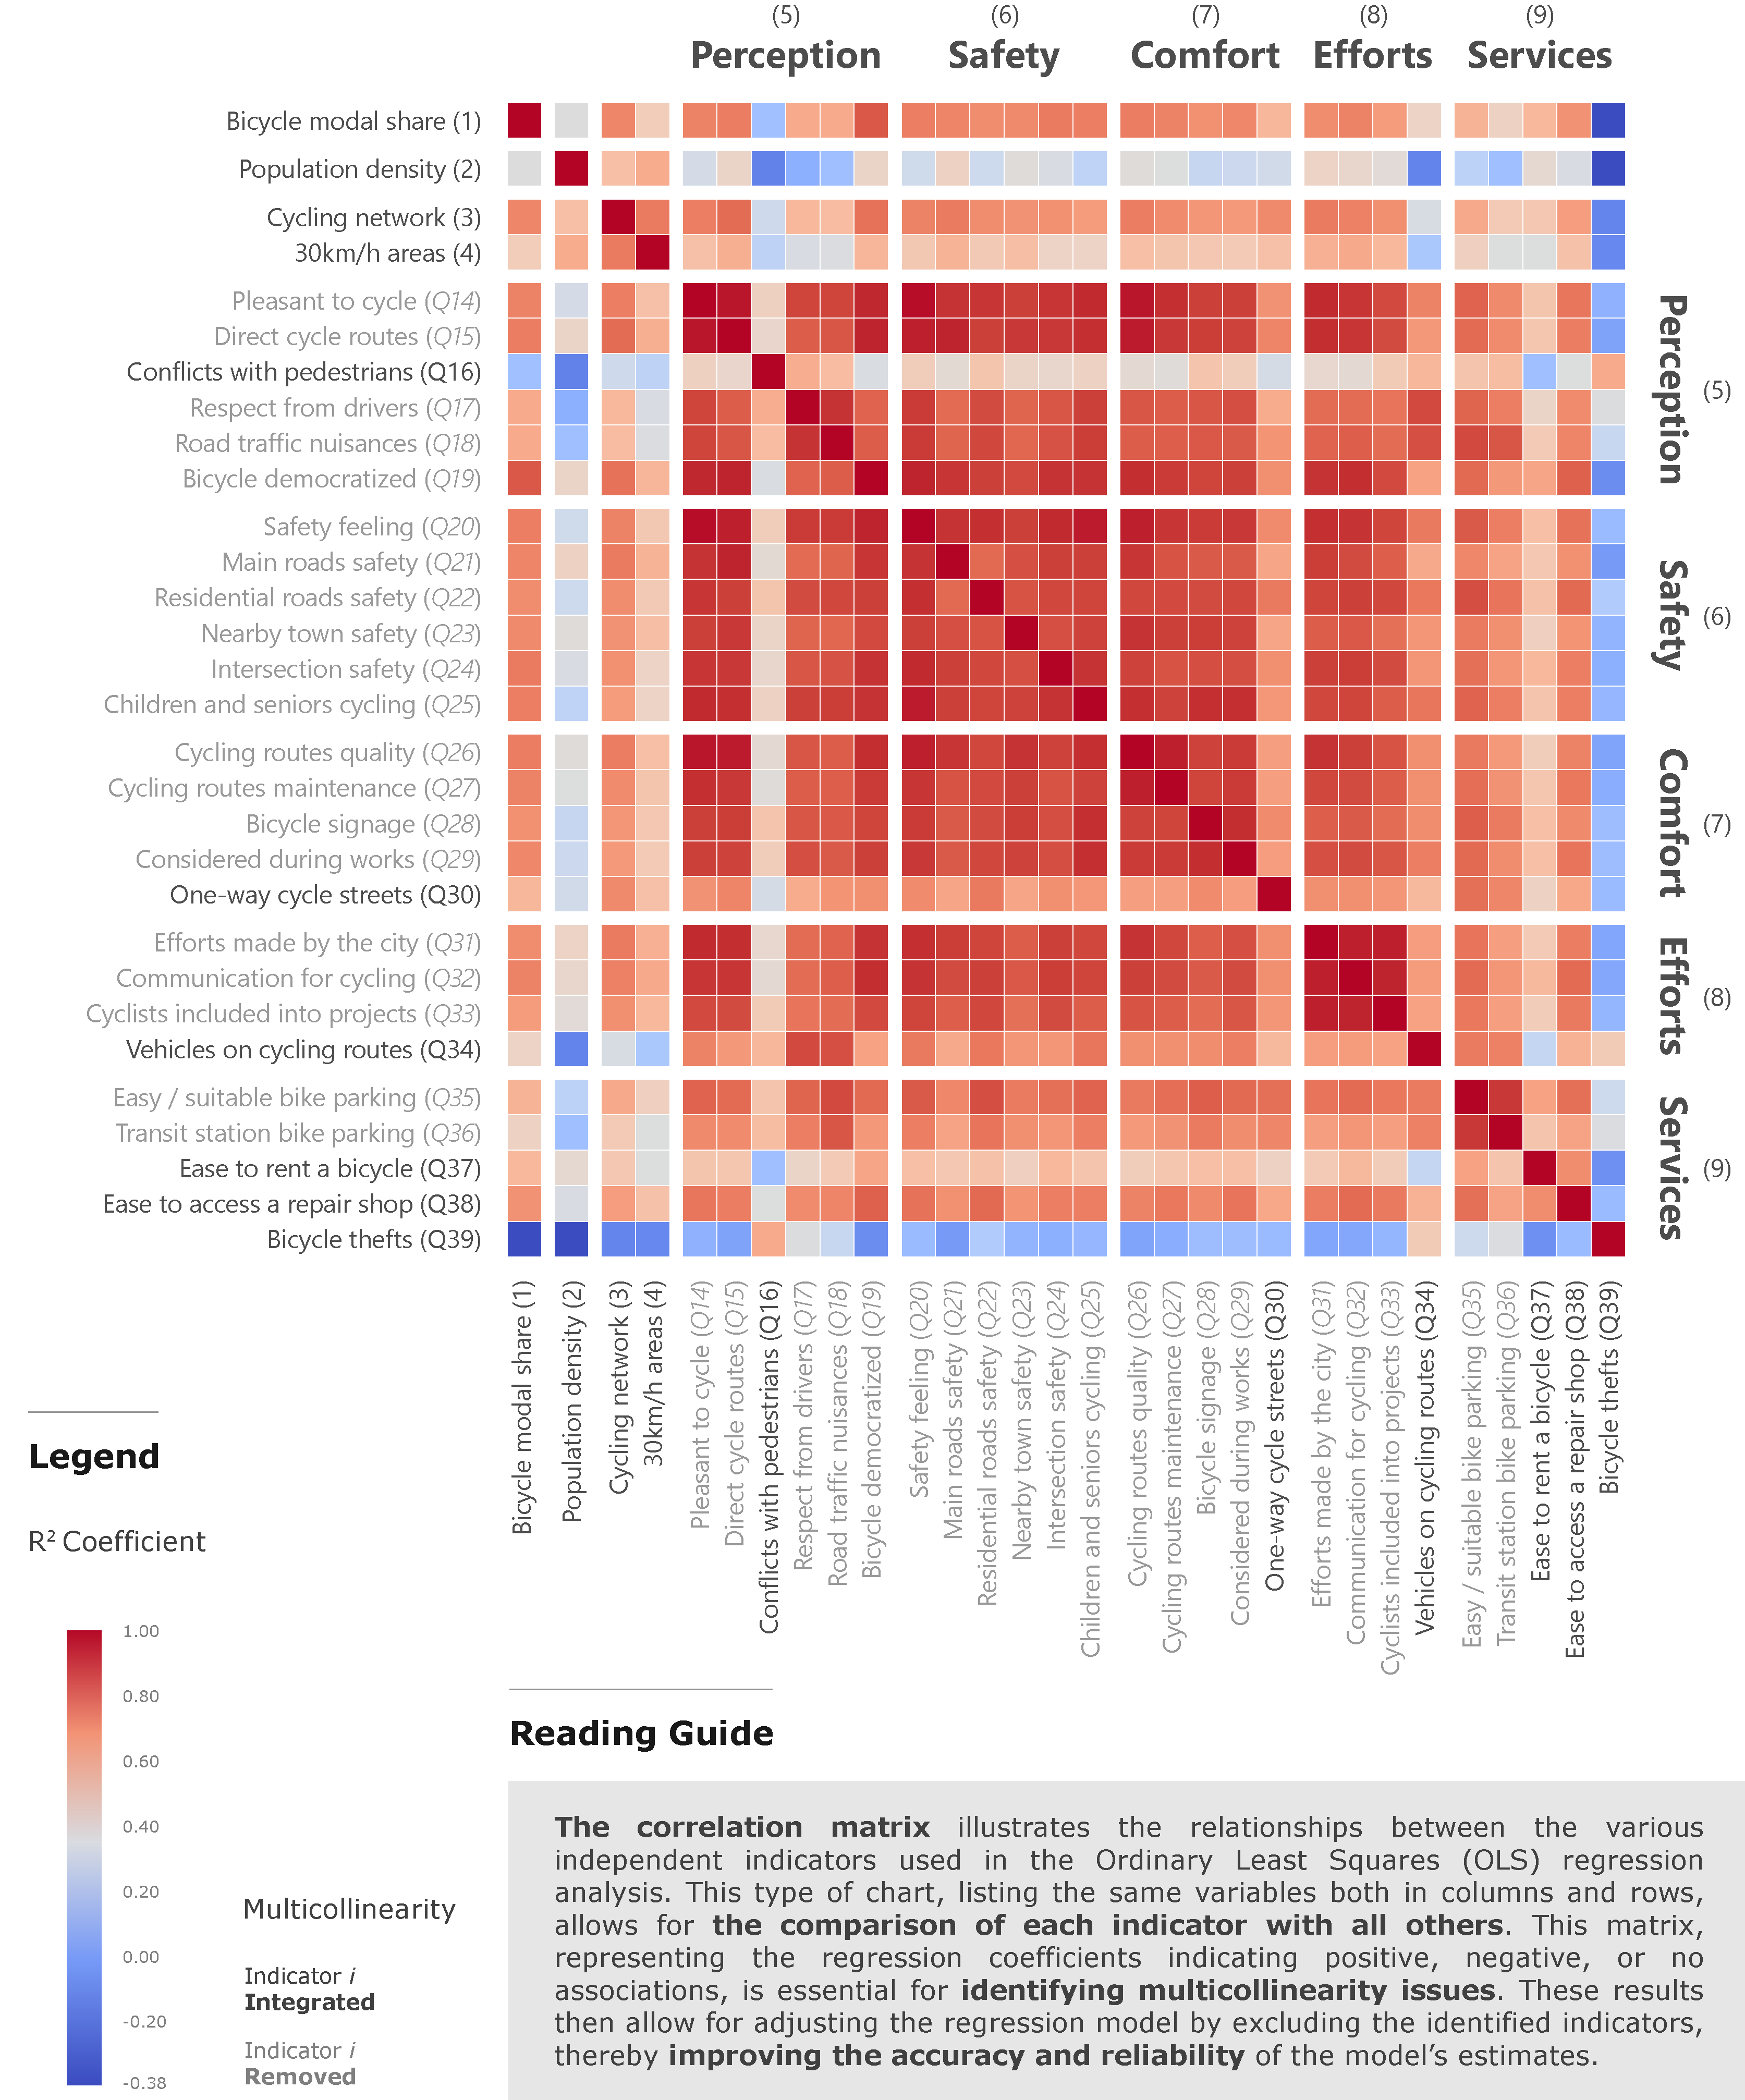
\includegraphics[width=1\columnwidth]{src/Figures/Chap-4/EN_Matrice_Autocorrelation_OLS.pdf}}
    \vspace{5pt}
    \begin{flushright}\scriptsize{
    Author: \textcolor{blue}{Dylan Moinse (2023)}
    }\end{flushright}
\end{figure}

%% Exclusion of Columns
The database used contains several pairs of highly correlated variables (\(VIF\)\textless10). We then chose to exclude 21 indicators from the model, as they were highly correlated with several other variables (see \hyperref[fig-chap4:matrice-autocorrelation]{Figure~\ref{fig-chap4:matrice-autocorrelation}}, page~\pageref{fig-chap4:matrice-autocorrelation}). In this context, we retained independent columns such as the \Commas{modal share of cycling} (\(T_{1}\)), the \Commas{average population density} (\(T_{2}\)), the \Commas{proportion of cycling routes} (\(T_{3}\)), the \Commas{proportion of areas where motorized speed is limited to 30 km/h} (\(T_{4}\)), as well as the scores for \Commas{general feeling} (\(T_{5}\)), \Commas{safety} (\(T_{6}\)), \Commas{comfort} (\(T_{7}\)), related to \Commas{city efforts} (\(T_{8}\)), \Commas{services and parking} (\(T_{9}\)), \Commas{conflicts with pedestrians} (\(Q_{16}\)), \Commas{one-way cycling streets} (\(Q_{30}\)), \Commas{vehicles on bike lanes} (\(Q_{34}\)), \Commas{ease of bike rental} (\(Q_{37}\)), \Commas{ease of access to a repair workshop} (\(Q_{38}\)), and \Commas{bike thefts} (\(Q_{39}\)). %%Translated%%

%% Transition
In this section dedicated to regression modeling, we systematically prepared the data and validated the key regression assumptions. Our analysis confirms that the regression model meets the assumptions of normality of residuals, homoscedasticity, and the absence of autocorrelation. By addressing these fundamental elements in statistics, we improve the overall interpretability of our results. %%Translated%%

% 4.3.2.2.
\needspace{1\baselineskip} % Reserve space
\subsubsection*{Model Validation
    \label{chap4:methodologie-validation}
    }

%% Introduction
To assess the predictive performance of our \acrshort{OLS} regression model, we calculated the \acrfull{MSE}. The \acrshort{MSE} is a \gls{metric} commonly used to evaluate the performance of regression models \textcolor{blue}{\autocite{cochran_sampling_1963}}\index{Cochran, William~G.|pagebf}. It is determined as the average of the squared differences between the predicted values and the actual values. %%Translated%%

%% Validation
The \acrshort{MSE} factor obtained is an extremely low value of 0.00127. This indicates that the model's predictions are very close to the actual values. A low \acrshort{MSE} is indeed desirable, as it signifies minimal forecasting errors, thus reflecting a high level of model accuracy. %%Translated%%

%% Coefficient
The multivariate \acrshort{OLS} regression model results in a regression coefficient ($R^2$) of 0.765 and an adjusted regression coefficient ($\bar{R}^2$) of 0.670, suggesting a good model fit. This means that 76.5\% of the variance in the dependent variable, namely the feminization rate of cycling practice, is explained by the independent variables included in the model. %%Translated%%

% 4.3.3.
\needspace{1\baselineskip} % Reserve space
\subsection{Bikeability in Relation to the Gendered Practice of Light Individual Mobility
    \label{section-chap4:cyclabilite-territoires-genre}
    }

%% Objectives
This section dedicated to mobility and gender aims to explore the existing relationships between the use of bicycles and micromobility, the urban environment, and gender, based on bikeability as perceived by cyclists. To this end, a series of predefined objectives guide this statistical investigation, as follows:
\begin{enumerate}
    \item First, this study focuses on quantifying gender inequalities concerning the use of light individual mobility from the perspective of daily mobility. This study seeks to rely on a large sample of individuals across a defined geographic area;
    \item Once the picture is drawn, the analysis questions the actual role played by \Commas{safety in numbers}\footnote{~
In the context of active mobility, \Commas{safety in numbers} is a concept suggesting that the more cyclists there are, the safer this mobility practice becomes for each user. This phenomenon can partly be explained by increased visibility on the road, prompting motorists to adopt safer driving behaviors, but also by better integration into planning policies and a snowball effect, where a certain critical mass encourages new people to adopt cycling, thereby improving safety in numbers retrospectively.
} in understanding the unequal distribution of micromobility usage;
    \item Following this statistical exploration, the evaluation of perceived bikeability as a parameter influencing the modal choice of light individual mobility helps shed light on mobility choices through the lens of gender;
    \item Through a comparative approach, this subsection seeks to characterize and classify the studied territories, in order to better contextualize the stated results;
    \item The final objective aims to develop an indicator capable of capturing the main interactions between the examined variables and the differentiated use of bicycles and micromobility. This index serves as an analytical tool, revealing the mechanisms underlying the gendered distribution in the use of light individual mobility.
\end{enumerate} %%Translated%%

%% Introduction
This section aims to present the results that emerge from this statistical analysis, highlighting the factors contributing to greater equity in the use of bicycles and micromobility. First and foremost, this research focuses on the gender disparities prevalent in France, as well as in our regional study, regarding the adoption of light individual mobility, whether it be cycling or emerging micromobility, both in monomodal and intermodal contexts. From this observation, we will attempt to demonstrate how the concept of \Commas{safety in numbers} is linked to understanding this social phenomenon, though without claiming it to be the direct factor. Indeed, this statistical analysis will emphasize the importance of the perceived bikeability by users, starting with the role of cycling infrastructure and safety, elements that depend on a set forming what can be called the \Commas{cycling system}. %%Translated%%

% 4.3.3.1.
\needspace{1\baselineskip} % Reserve space
\subsubsection*{A Clear Gender Gap in the Use of Bicycles and Micromobility in France
    \label{chap4:ecart-genre}
    }

%% Gendered Monomodal Use
The central focus of this subsection is the measurement of the gendered distribution of bicycle and micromobility use in France. Not surprisingly, the secondary analysis of the \textsl{MOBPro} file highlights a significant demographic imbalance regarding bicycle use. This national mobility database reveals that female participation in cycling accounts for only 38.08\% of users for home-to-work trips in the country, as shown in the \hyperref[fig-chap4:part-modale-genree-mobilite-individuelle-legere]{Figure~\ref{fig-chap4:part-modale-genree-mobilite-individuelle-legere}} (page~\pageref{fig-chap4:part-modale-genree-mobilite-individuelle-legere}), even though women make up 51.60\% of the French population \textcolor{blue}{\autocite{insee_documentation_2023}}\index{Insee@\textsl{Insee}|pagebf} and 58\% of rail passengers \textcolor{blue}{\autocite{enov_enquete_2021}}\index{Enov@\textsl{Enov}|pagebf}. %%Translated%%

%% Figure Gender and Types of Micromobility
\begin{figure}[h!]\vspace*{4pt}
    \caption{Distribution of bicycle and micromobility use by declared and observed gender.}
    \label{fig-chap4:part-modale-genree-mobilite-individuelle-legere}
    \centerline{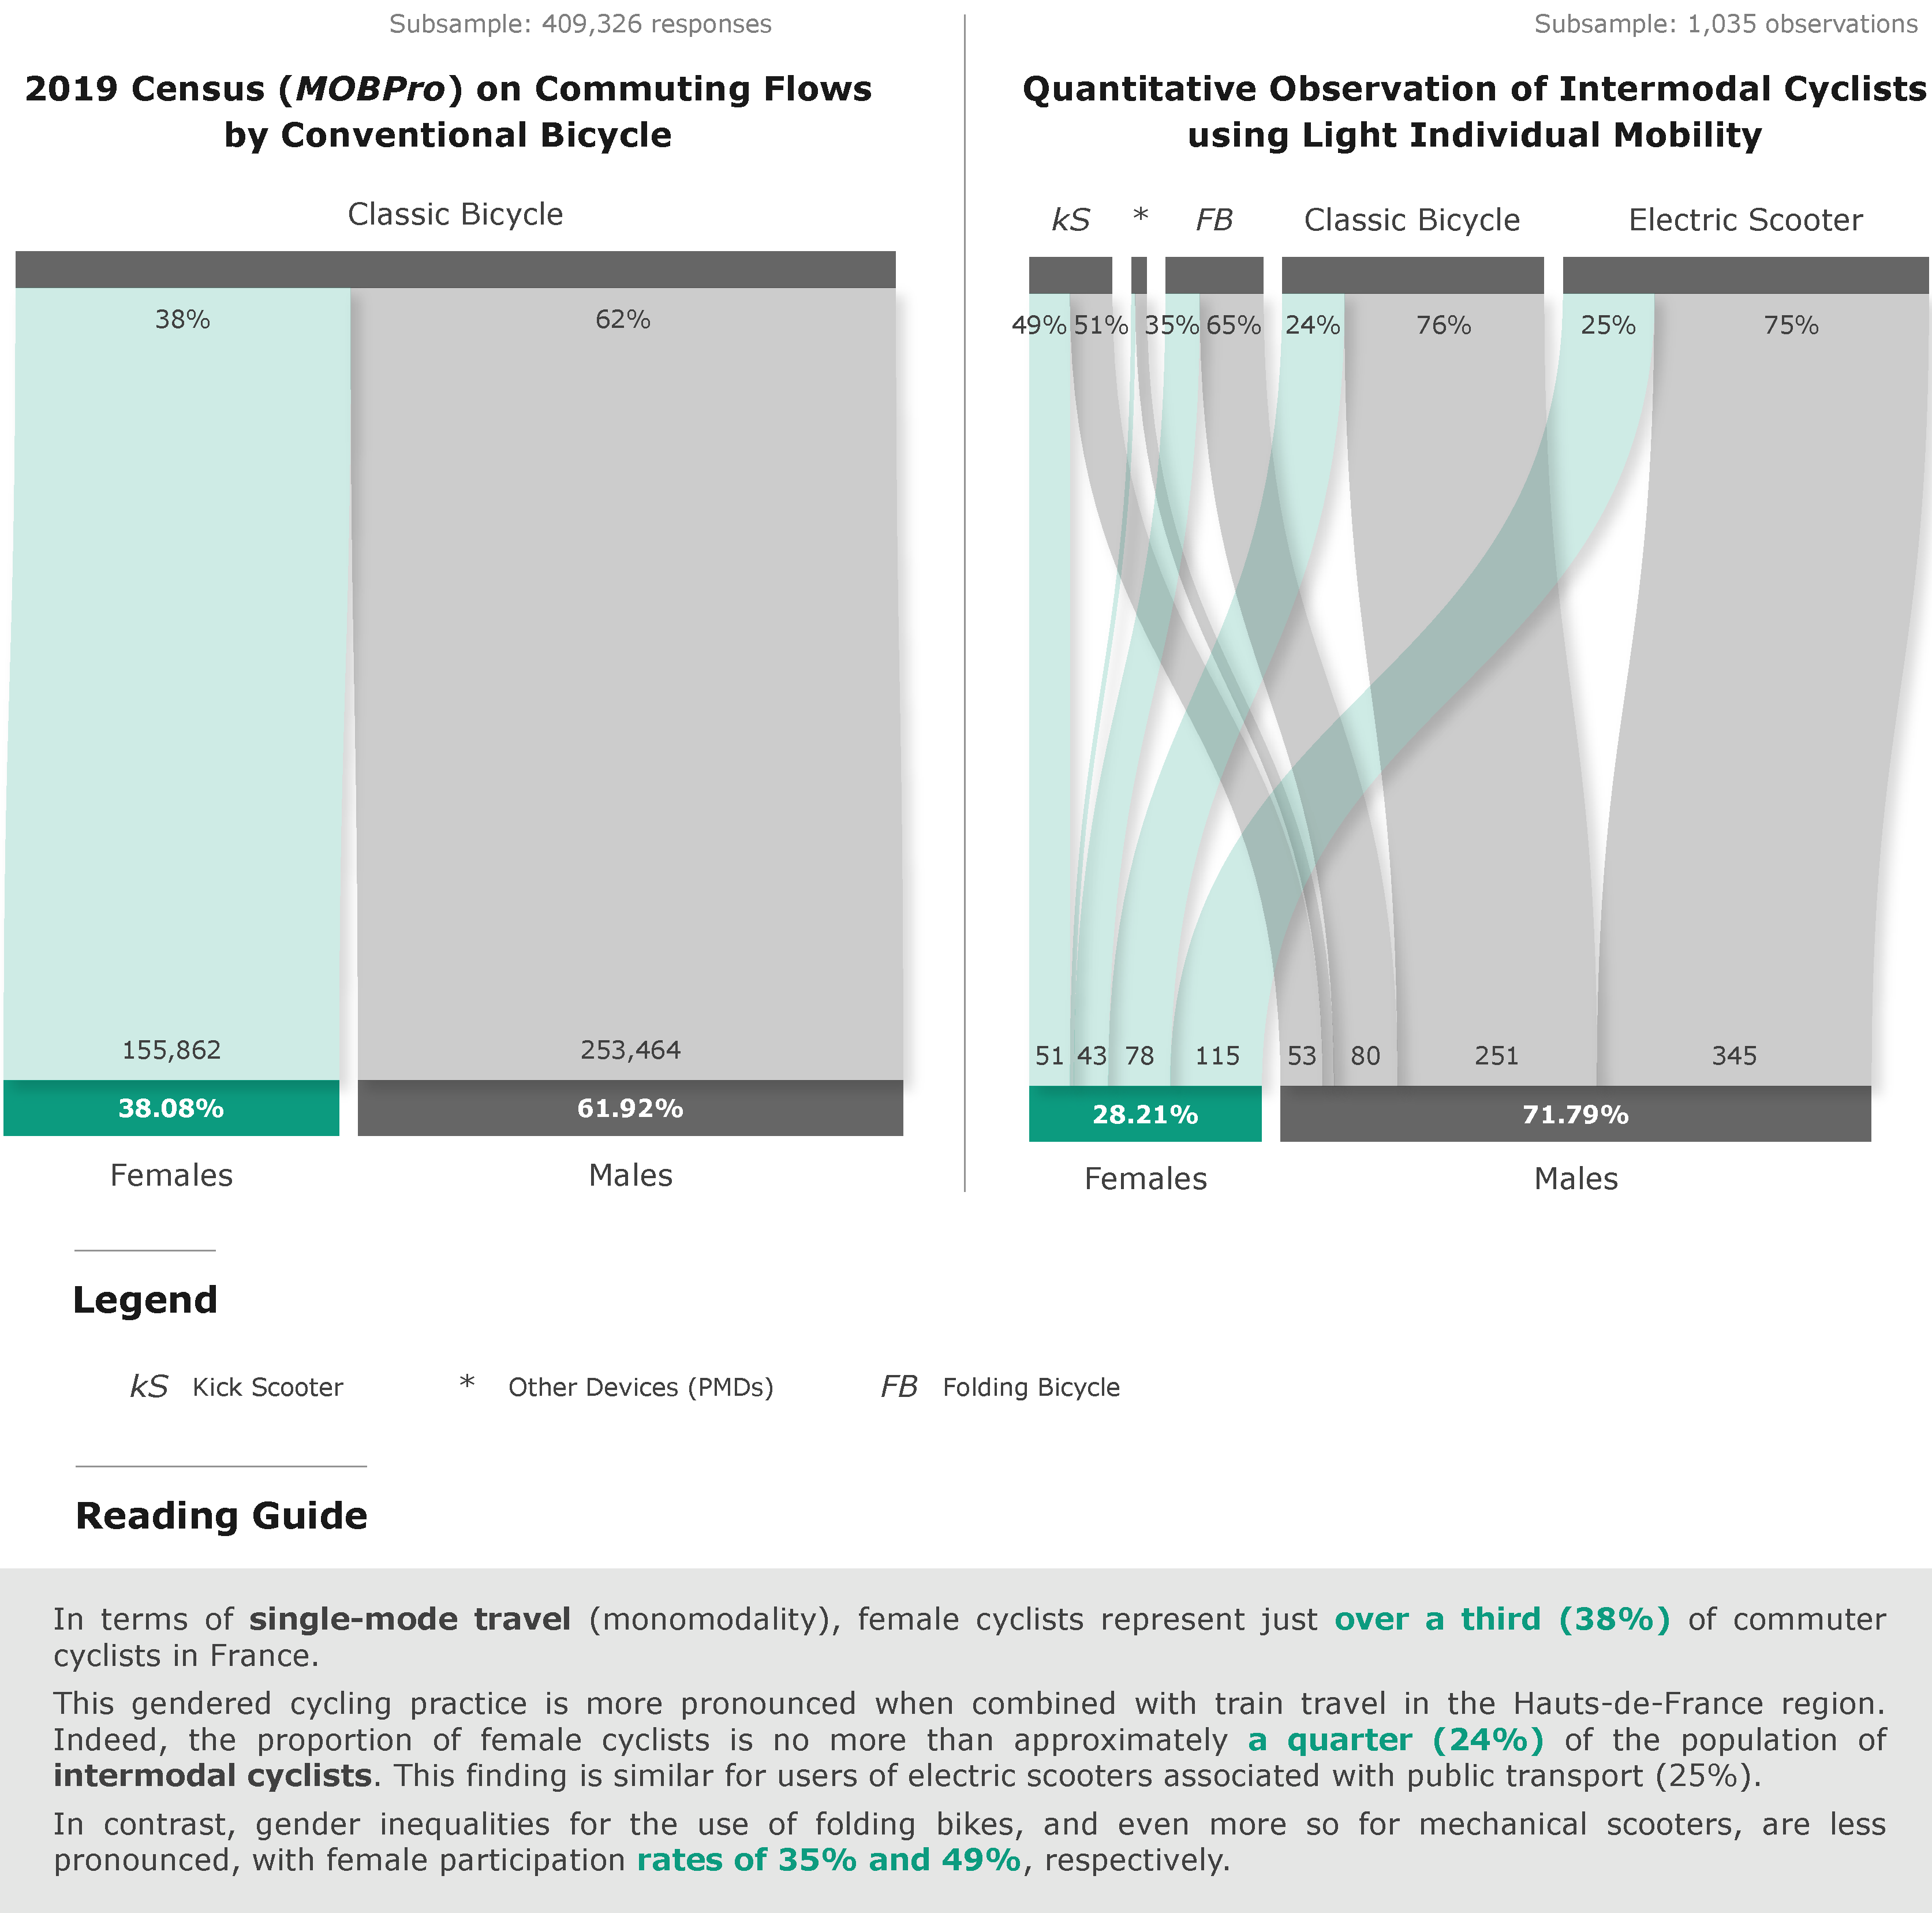
\includegraphics[width=1\columnwidth]{src/Figures/Chap-4/EN_Part_modale_genre_OLS.pdf}}
    \vspace{5pt}
    \begin{flushright}\scriptsize{
    Datasets: \textsl{MOBPro} \textcolor{blue}{\autocite{insee_documentation_2023}}
    \\
    Author: \textcolor{blue}{Dylan Moinse (2023)}
    }\end{flushright}
\end{figure}

% 4.3.3.2.
\needspace{1\baselineskip} % Reserve space
\subsubsection*{The Indirect Role of Critical Mass of Cyclists in Reducing Gender Inequalities
    \label{chap4:masse-critique-genre}
    }

%% Modal Share and Gendered Use
This statistical evaluation first examines, at the national level, the links between female participation rates and the modal share of cycling in fifty-three French cities. The multivariate regression model highlights the relatively significant positive correlation between the percentage of women cycling and the widespread use of cycling in central cities, with a coefficient of determination (denoted $\hat{\beta}_{1}$) of 0.37 ($p$\textless0.05). The concept of \Commas{safety in numbers} involves recognizing that the more cyclists there are in public spaces, the more motorists tend to consider them as a legitimate group of road users. As a result, motorists become more attentive to cyclists, as explained by \textcolor{blue}{\textcite[83]{oosteren_pourquoi_2021}}\index{Oosteren, Stein van|pagebf}\index{Schneider, Olivier|pagebf}, since the relationship between the total number of cyclists and the number of cyclists involved in road accidents is inversely proportional \textcolor{blue}{\autocite[208]{jacobsen_safety_2003}}\index{Jacobsen, Peter Lyndon|pagebf}. %%Translated%%

%% Figure Gender and Modal Share of Cycling
\begin{carte}[h!]\vspace*{4pt}
    \caption{Cross-analysis of the modal share and the gender distribution of bicycle use in France.}
    \label{fig-chap4:carte-part-modale-velo-genre}
    \centerline{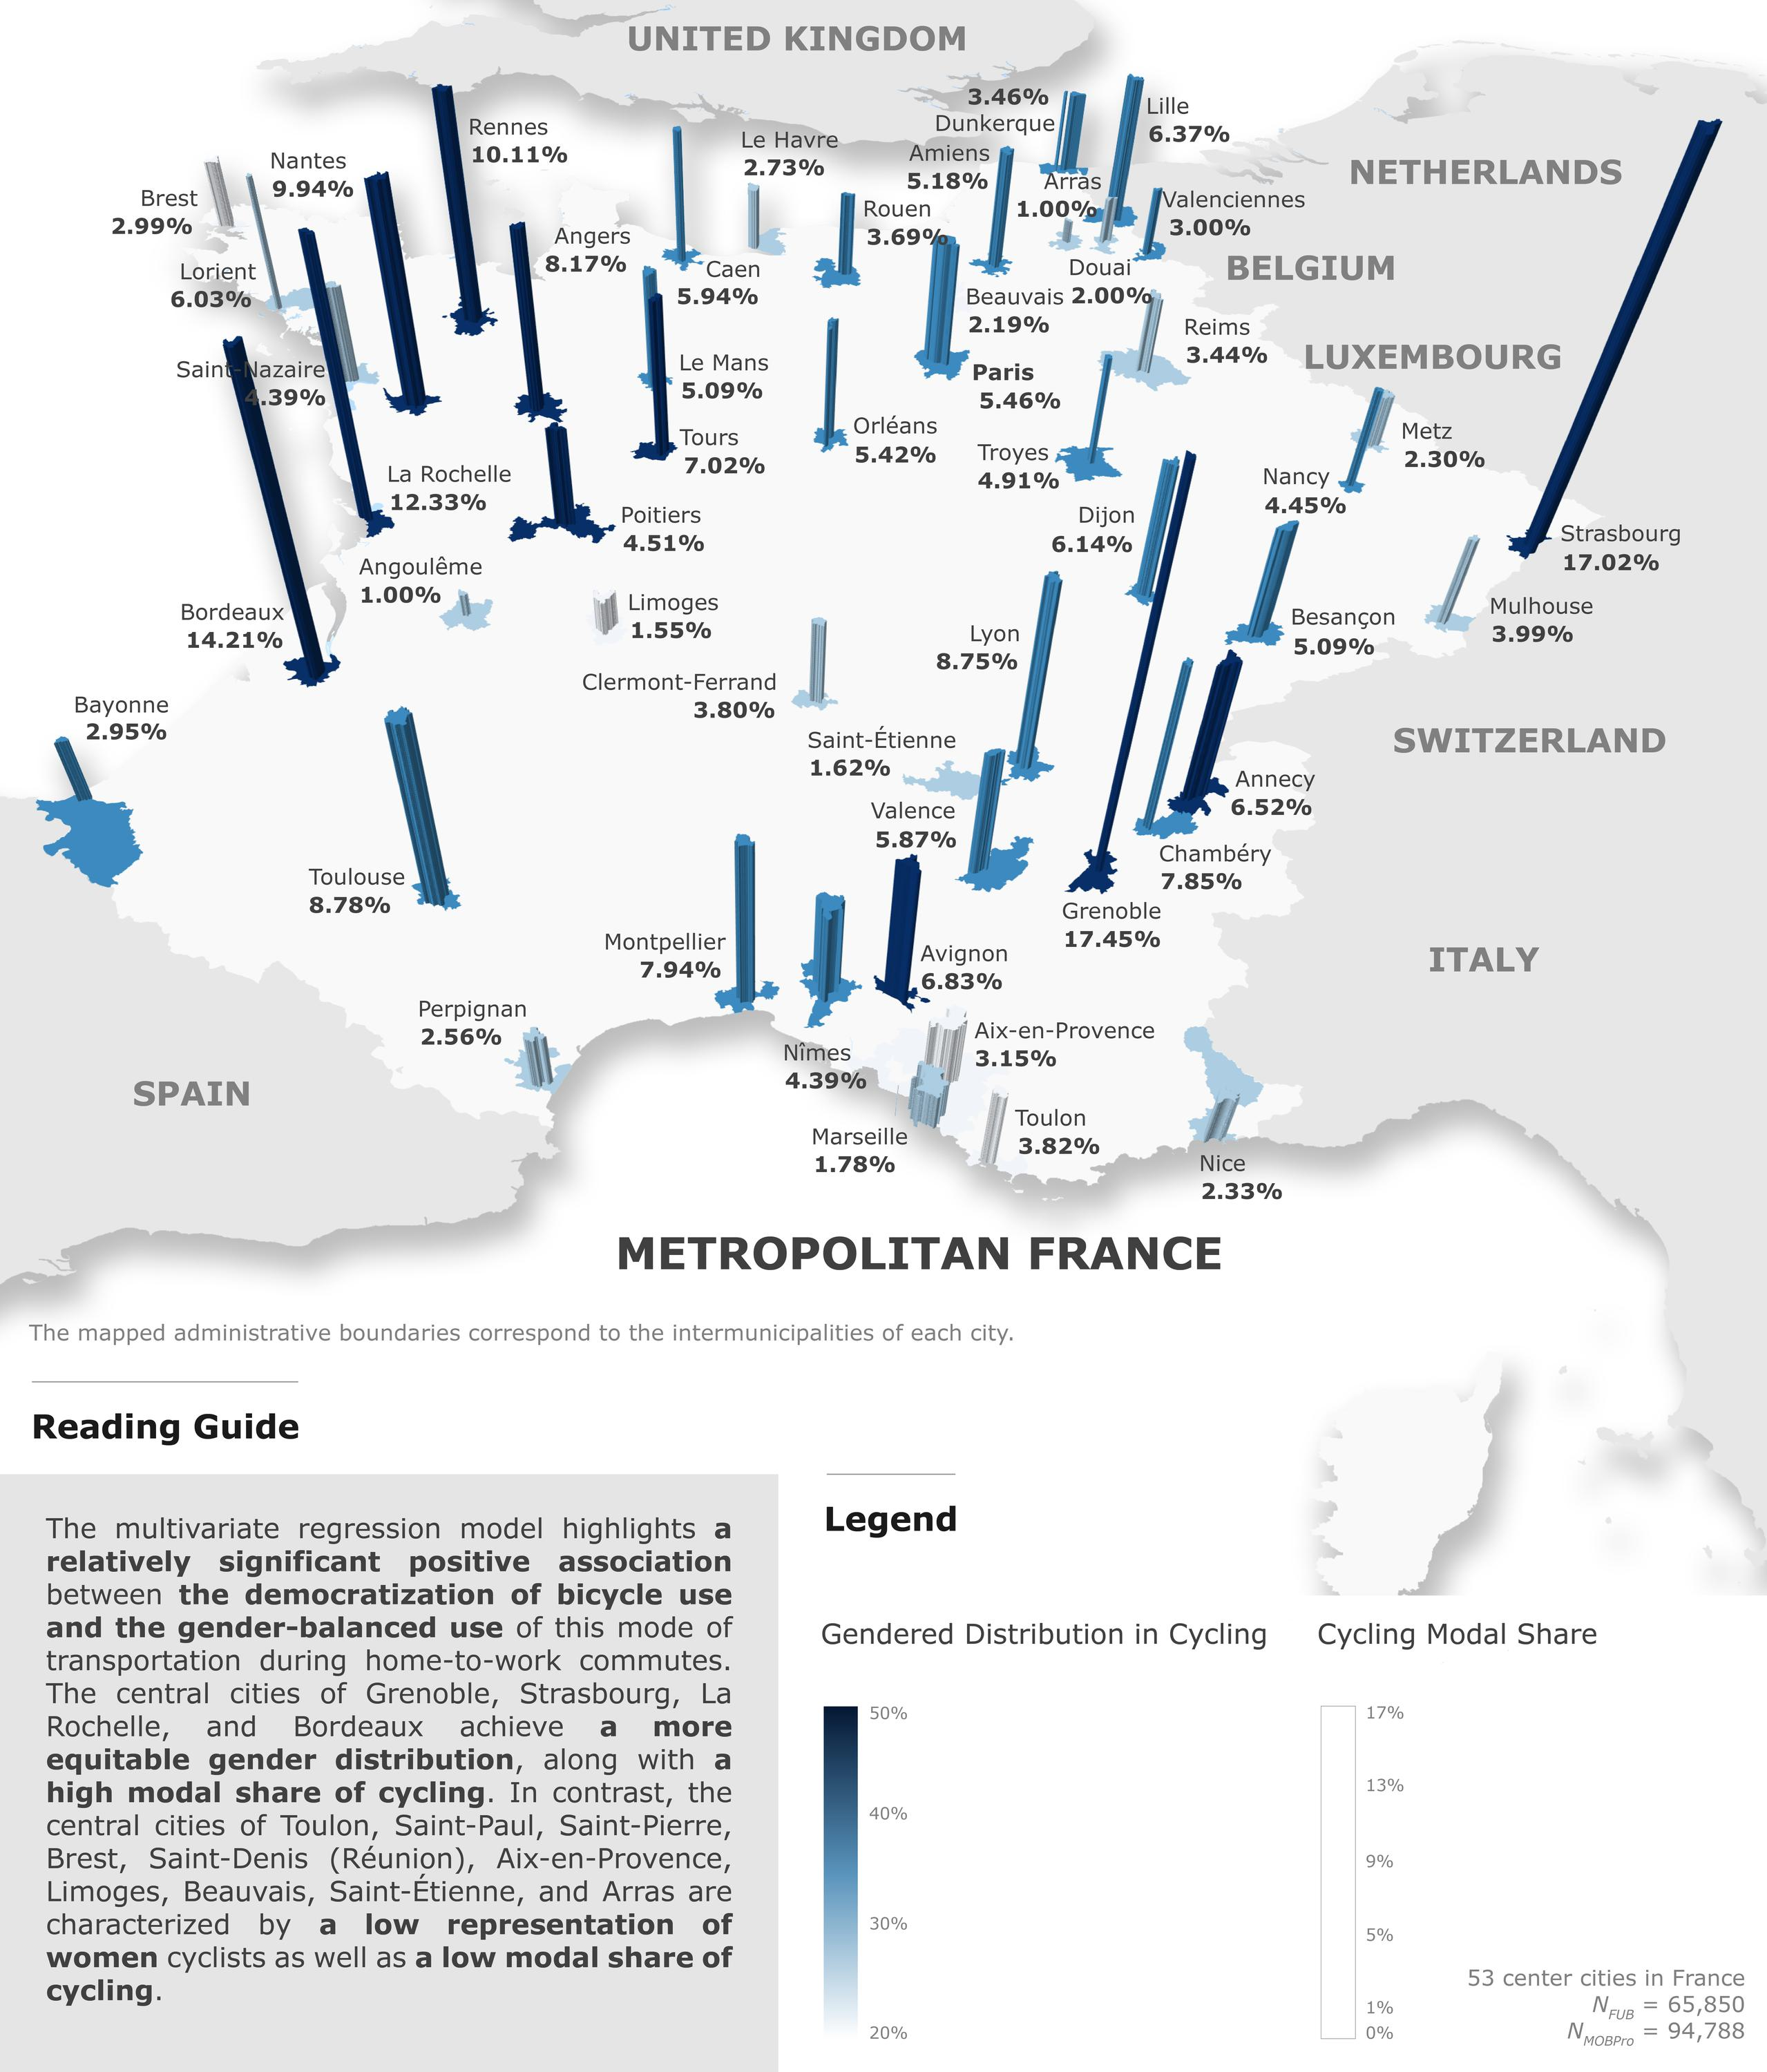
\includegraphics[width=1\columnwidth]{src/Figures/Chap-4/EN_Democratisation_velo_genre_OLS.jpg}}
    \vspace{5pt}
    \begin{flushright}\scriptsize{
    Datasets: \textsl{MOBPro} \textcolor{blue}{\autocite{insee_documentation_2023}} and \textsl{Regional Bicycle Atlas} \textcolor{blue}{\autocite{velo__territoires_atlas_2023}}
    \\
    Author: \textcolor{blue}{Dylan Moinse (2023)}
    }\end{flushright}
\end{carte}

%% Examples of Good Scores
In the field of cities renowned for their significant development in terms of cycling in France, particularly regarding the proportion of active individuals who choose cycling, it is important to highlight a more equitable gender distribution. Notably, in Grenoble and Strasbourg, where the modal share reaches about 17\%, we can observe a nearly balanced gender representation in this mode of transport, with figures of approximately 45\% and 49\% respectively (see \hyperref[fig-chap4:carte-part-modale-velo-genre]{Map~\ref{fig-chap4:carte-part-modale-velo-genre}}, page~\pageref{fig-chap4:carte-part-modale-velo-genre}). Similarly, La Rochelle and Bordeaux achieve a gender parity closely aligned with their municipal population (51\%), while displaying modal shares of cycling of around 12\% and 14\%. %%Translated%%

%% Examples of Poor Scores
Conversely, some cities are characterized by a low modal share of cycling, below the national average of 3.5\%, combined with a low representation of female cyclists. Among the most unequal cities are Toulon (20\%), Saint-Paul (22\%), Saint-Pierre (24\%), Brest (25\%), Saint-Denis de La Réunion (25\%), Aix-en-Provence (26\%), Limoges (26\%), Beauvais (28\%), Saint-Étienne (28\%) and Arras (28\%), where the modal share of cycling ranges from 1\% to 3\% (see \hyperref[fig-chap4:carte-part-modale-velo-genre]{Map~\ref{fig-chap4:carte-part-modale-velo-genre}}, page~\pageref{fig-chap4:carte-part-modale-velo-genre}). However, it is necessary to nuance these observations by considering specific counterexamples that do not seem to follow this linear regression model. Cities such as Avignon (50\%), Poitiers (45\%), Valenciennes (42\%) and Bayonne (37\%) stand out for having less pronounced gender disparities, despite a modest modal share of cycling, ranging between 3\% and 7\%. %%Translated%%

%% Quantitative Observation
The positive correlation determined between the modal share and female participation in cycling remains consistent but appears much less significant when considering the intermodal use of micromobility in the Hauts-de-France case study. The linear regression model produces a coefficient of 0.25 ($p$\textless0.05) when analyzing data from the nine surveyed train stations. At the central Lille Flandres station and the suburban Lille CHR station, where the modal share of cycling in the municipality is 6.1\%, less than a third of the travelers using this intermodal combination with conventional bicycles are women (31.70\% out of 287 observations and 31.97\% out of 122 observations). A similar gender distribution is observed at the Armentières station (31.72\% out of 145 observations) in a municipality where 4\% of commuters cycle. The trend curve is then influenced by the stations of Béthune (21.88\% out of 32 observations), Lesquin (15.79\% out of 22 observations), Creil (12.5\% out of 32 observations), and Dunkirk (12.24\% out of 49 observations), where the modal share of cycling ranges from 1\% to 3\%. When differentiating between types of light individual mobility, a moderately significant relationship is observed ($\hat{\beta}$~=~0.23,~$p$\textless0.05) for the intermodal use of conventional bicycles, while a weak relationship is found for \acrshort{PeS} combined with public transport networks ($\hat{\beta}$~=~0.17,~$p$\textless0.05). However, this relationship is not significant for folding bicycles and mechanical scooters. At this point, we propose to confront the quantitative analysis with the assessments made through our qualitative protocol. %%Translated%%

%% Commented Routes
The primacy given to the concept of \Commas{safety in numbers} in the practice of light individual mobility is evident in the examination of the commented routes implemented. The participant designated as \(PCTE_{1}\) presents a nuanced perspective regarding the coexistence of \acrshort{PeS} users with automobile traffic in the neighborhood areas near train stations. This participant identifies the sharing of the roadway as a major obstacle to the adoption of this mode of transport. The participant compares various mobility experiences, highlighting a gradual familiarization of motorists with the \acrshort{PeS}, \Commas{\textsl{getting used to this mode of transport}} [17:40, \(PCTE^{TC}_{1}\)] in the Lille context. These interactions contrast sharply with her feelings in Maubeuge, where the user expresses a sense of insecurity and disconnection, saying she \Commas{\textsl{feels like an alien}} in this urban environment [17:40, \(PCTE^{TC}_{1}\)]. The mention of cyclist visibility reappears during her description of her route in egress in Maubeuge, where the participant insists that \Commas{\textsl{the cars are not hyper used to things like scooters or bicycles. It's a small bike lane going uphill, but I'm afraid the cars won't pay attention}}. This testimony, in addition to reinforcing the importance of critical mass of cyclists in public spaces, shows that the mere presence of bike lanes does not make the participant feel safe on an electric scooter (see \hyperref[fig-chap4:pcte1e-partage-voirie]{Figure~\ref{fig-chap4:pcte1e-partage-voirie}}, page~\pageref{fig-chap4:pcte1e-partage-voirie}). However, she mentions the presence of a few electric scooter users in the municipality, an observation that \Commas{[reassures her]. [\dots] \textsl{motorists are a little bit familiar with} [scooters traveling on the road]. \textsl{Even though there aren't that many bikes alone.}} [17:40, \(PCTE^{TC}_{1}\)]. %%Translated%%

%% Figure 1 PCTE1E Maubeuge
\begin{figure}[h!]\vspace*{4pt}
    \caption{Image extracted from the filmed route broadcast from the Maubeuge train station, illustrating the presence of a turn deemed dangerous at the end of the path (\(PCTE^{E}_{1}\)).}
    \label{fig-chap4:pcte1e-partage-voirie}
    \centerline{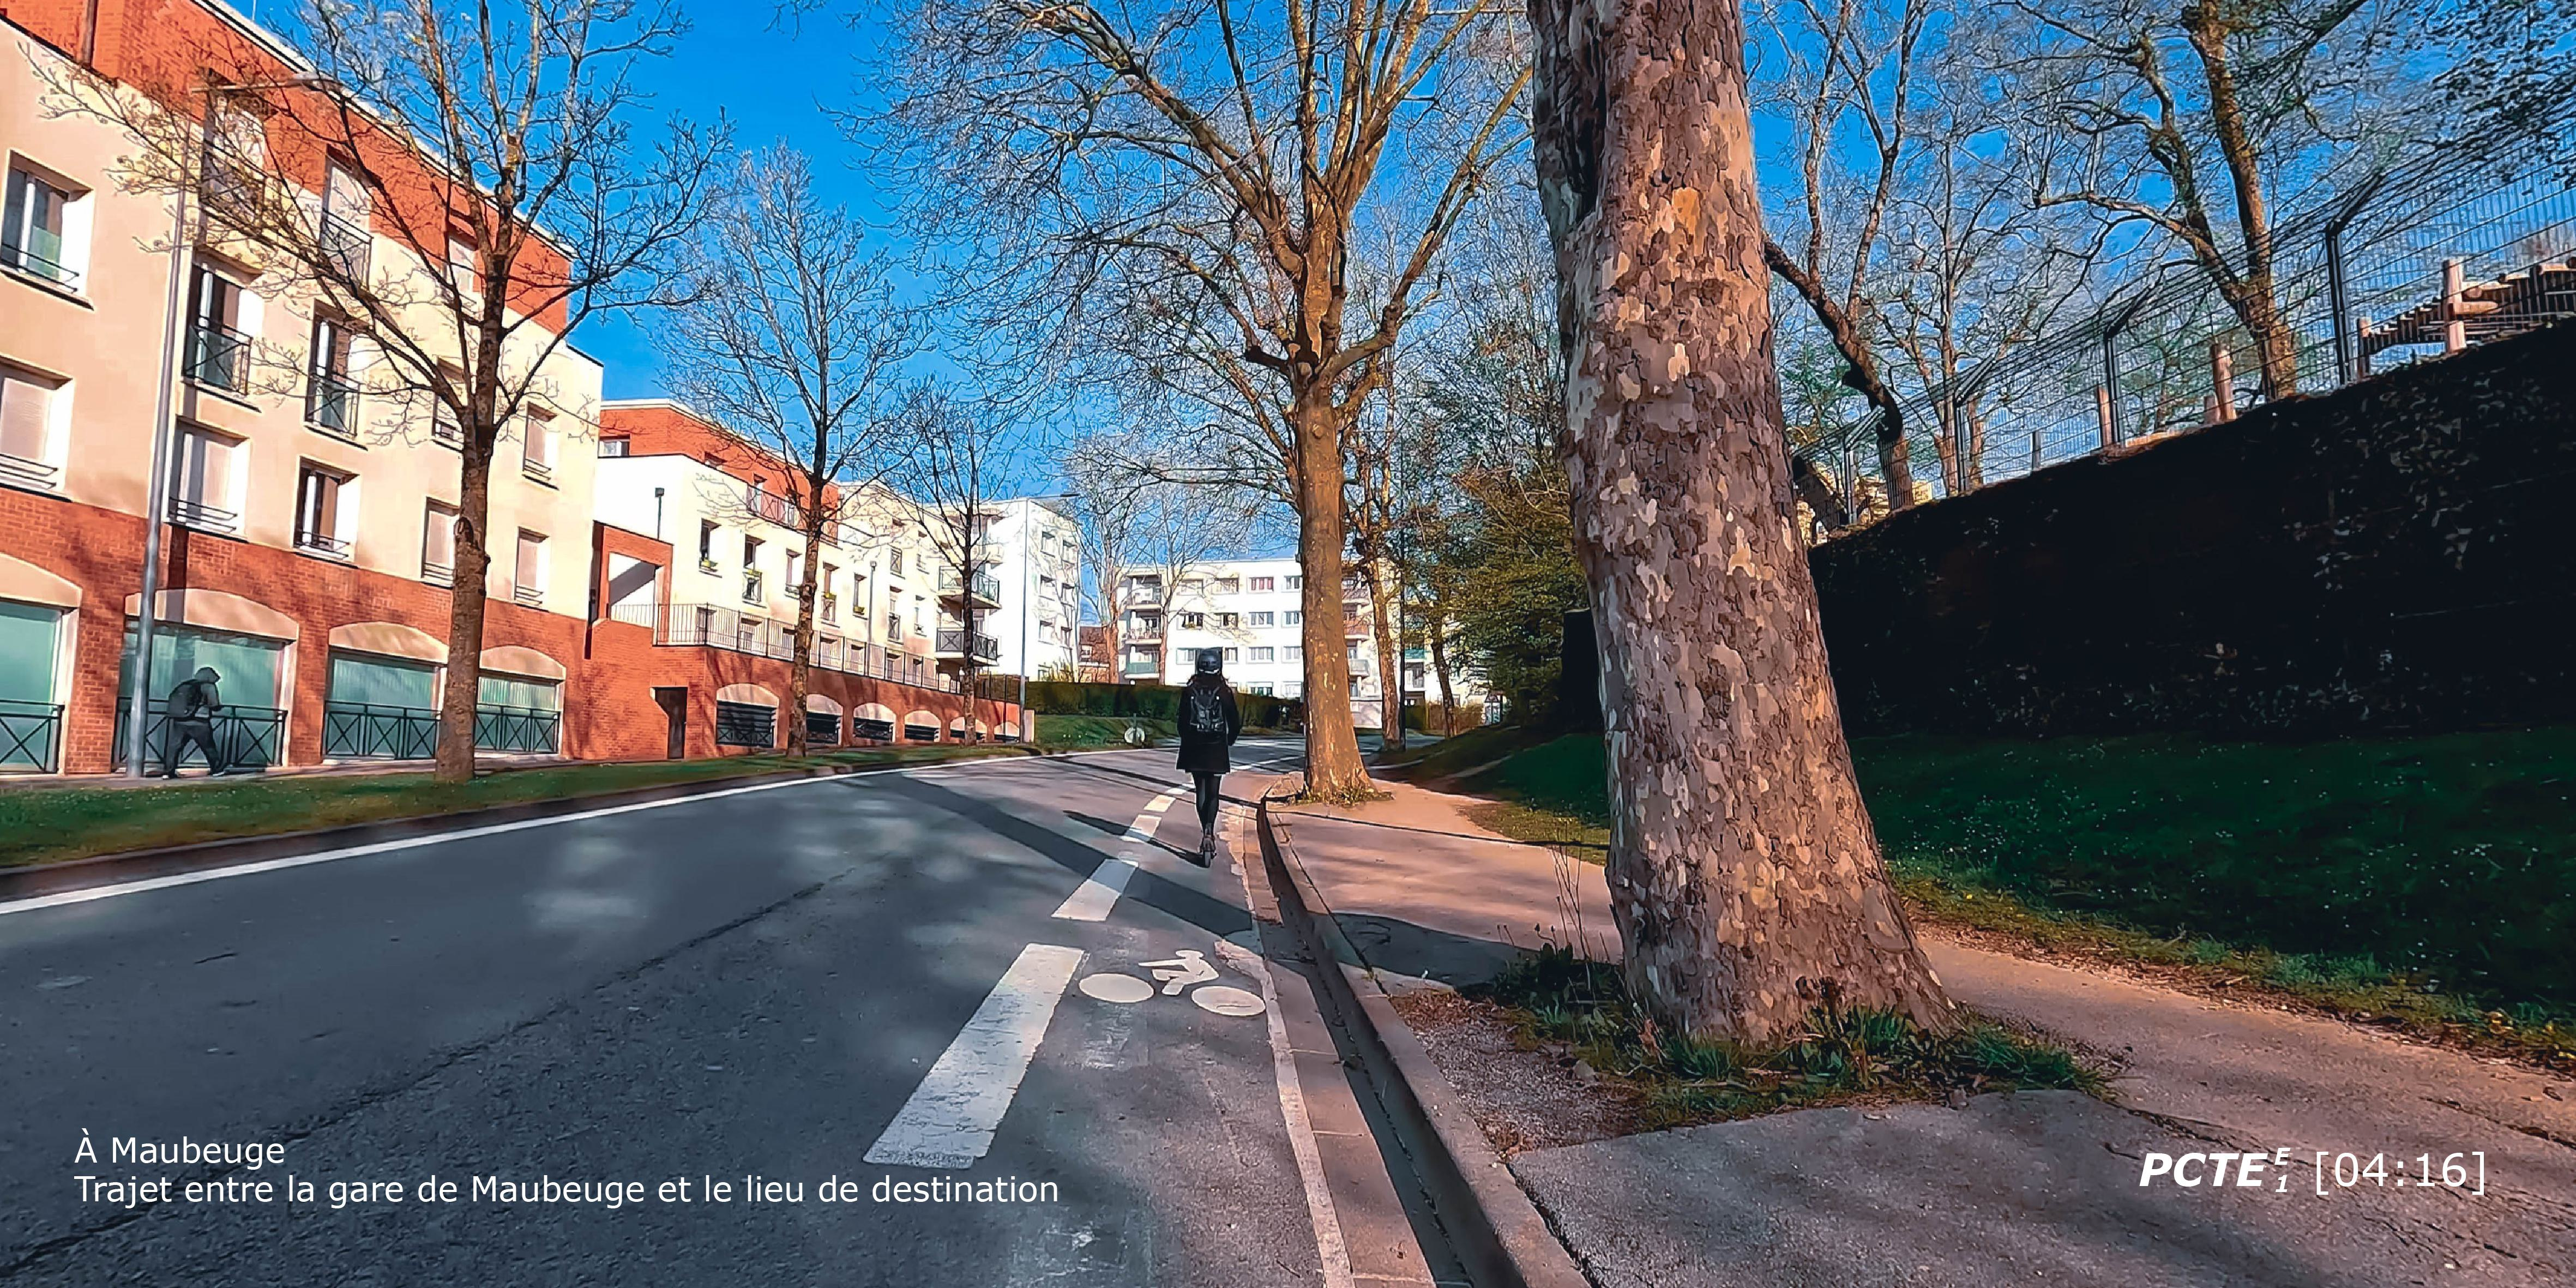
\includegraphics[width=1\columnwidth]{src/Figures/Chap-4/Extrait_Video_PCTE1_Egress_9.jpg}}
    \vspace{5pt}
    \begin{flushright}\scriptsize{
    Author: \textcolor{blue}{Dylan Moinse (2022)}
    }\end{flushright}
\end{figure}

%% Literature Discussion
To our knowledge, the critical role of the critical mass of cyclists in female participation in light individual mobility has not yet been statistically demonstrated in the French context, except in Strasbourg, where the modal share of cycling exceeds 17\% and women represent 48\% of cyclists \textcolor{blue}{\autocite[42]{certu_usagers_2013}}\index{Certu@\textsl{Certu}|pagebf}. Some observations made by \textcolor{blue}{Frédéric} \textcolor{blue}{\textcite[187]{heran_retour_2015}}\index{Héran, Frédéric|pagebf} and \textcolor{blue}{Thibaut} \textcolor{blue}{\textcite{schepman_pourquoi_2014}}\index{Schepman, Thibaut|pagebf} suggest that a strong presence of cyclists in a municipality tends to promote a more equitable use of bicycles, citing examples such as Strasbourg and Copenhagen. These results are consistent with the international comparison conducted by \textcolor{blue}{\textcite[63]{garrard_revolutions_2006}}\index{Garrard, Jan|pagebf}\index{Crawford, Sharyn|pagebf}\index{Hakman, Natalie|pagebf}, who highlighted that countries with high cycling usage rates, whether for commuting or leisure, tend to experience reduced gender differences in this form of active mobility. Similarly, in an analysis covering seventeen countries across six continents, \textcolor{blue}{\textcite[70]{goel_cycling_2022}}\index{Goel, Rahul|pagebf}\index{Goodman, Anna|pagebf}\index{Aldred, Rachel|pagebf}\index{Nakamura, Ryota|pagebf}\index{Tatah, Lambed|pagebf}\index{Garcia, Leandro Martin Totaro|pagebf}\index{Zapata-Diomedi, Belen|pagebf}\index{Sa, Thiago Herick de|pagebf}\index{Tiwari, Geetam|pagebf}\index{Nazelles, Audrey de|pagebf}\index{Tainio, Marko|pagebf}\index{Buehler, Ralph|pagebf}\index{Götschi, Thomas|pagebf}\index{Woodcock, James|pagebf} identified a positive correlation between the democratization of cycling and the tendency of women to cycle. Furthermore, in municipalities and countries where the modal share of cycling is below 7\%, women on average have a 56\% lower likelihood of cycling compared to men, as shown by \textcolor{blue}{\textcite[70]{goel_cycling_2022}}\index{Goel, Rahul|pagebf}\index{Goodman, Anna|pagebf}\index{Aldred, Rachel|pagebf}\index{Nakamura, Ryota|pagebf}\index{Tatah, Lambed|pagebf}\index{Garcia, Leandro Martin Totaro|pagebf}\index{Zapata-Diomedi, Belen|pagebf}\index{Sa, Thiago Herick de|pagebf}\index{Tiwari, Geetam|pagebf}\index{Nazelles, Audrey de|pagebf}\index{Tainio, Marko|pagebf}\index{Buehler, Ralph|pagebf}\index{Götschi, Thomas|pagebf}\index{Woodcock, James|pagebf}. %%Translated%%

%% Transition
This second phase of statistical analysis has established a significant link between the proportion of cyclists and the tendency of women to adopt cycling from a geographical perspective. However, this significant correlation does not provide indications about the causal relationships between these two variables. In particular, it remains uncertain whether the influence of critical mass actually favors greater gender diversity among cyclists, or if it is the increased participation of women that tends to raise the modal share of this mode of transport, or even a combination of both factors interacting. It is in this perspective, and within the framework of our scientific positioning concerning the role of territorial arrangement, that this study sought to assess the role of bikeability. %%Translated%%
    
% 4.3.3.3.
\needspace{1\baselineskip} % Reserve space
\subsubsection*{Addressing Gender Inequalities in Mobility in Light of Bikeability
    \label{chap4:cyclabilite-genre}
    }

    %% Associations related to urban environment
Through the comparative approach conducted in the 53 central cities, the regression model highlights a positive association between the gendered use of bicycles and the share of cycling infrastructure in each municipality ($\hat{\beta}_{3}$~=~0.60,~$p$\textless0.01). In contrast, the correlation between the share of 30 km/h zones and the gender distribution of cycling is not statistically significant ($\hat{\beta}_{4}$~=~-0.12,~$p$~\texttt{>}~0.10), similarly to the population density, which shows no discernible relationship ($\hat{\beta}_{2}$~=~-0.17,~$p$~\texttt{>}~0.10). The results thus confirm the significant links between the modal share of cycling and objective bikeability \textcolor{blue}{\autocite[8]{codina_built_2022}}\index{Codina, Oriol|pagebf}\index{Maciejewska, Monika|pagebf}\index{Nadal, Jordi|pagebf}\index{Marquet, Oriol|pagebf} that influence the gendered use of bicycles (see \hyperref[table-chap4:regression-genre-barometre-fub]{Table~\ref{table-chap4:regression-genre-barometre-fub}}, page~\pageref{table-chap4:regression-genre-barometre-fub}).%%Translated%%


    % Tableau Résultats de la régression OLS
% Results of the OLS Regression
%%Rédigé%%
    \begin{table}[h!]
    \centering
    \renewcommand{\arraystretch}{1.5}
    \resizebox{\columnwidth}{!}{
    \begin{tabular}{p{0.07\columnwidth}p{0.39\columnwidth}p{0.09\columnwidth}p{0.07\columnwidth}p{0.08\columnwidth}p{0.07\columnwidth}p{0.07\columnwidth}p{0.09\columnwidth}p{0.07\columnwidth}}
        %\hline
    \rule{0pt}{15pt} \small{\textcolor{blue}{\textbf{ID}}} & \small{\textcolor{blue}{\textbf{Independent Variables}}} & \small{\textcolor{blue}{\textbf{$\hat{\beta}$}}} & \small{\textcolor{blue}{\textbf{$\sigma$}}} & \small{\textcolor{blue}{\textbf{\(t_{stat}\)}}} & \small{\textcolor{blue}{\textbf{$p$}}} & \small{\textcolor{blue}{\textbf{\(VIF\)}}} & \small{\textcolor{blue}{\textbf{\(IC_{inf}\)}}} & \small{\textcolor{blue}{\textbf{\(IC_{sup}\)}}}\\
        \hline
\(T_{1}\) & \underline{\small{Modal share of cycling}} & \small{0.37} & \small{0.17} & \small{2.12} & \small{0.04} & \small{4.73} & \small{0.02} & \small{0.72} \\
\(T_{2}\) & \small{Population density} & \small{-0.17} & \small{0.14} & \small{-1.16} & \small{0.25} & \small{3.28} & \small{-0.46} & \small{0.13} \\
\(T_{3}\) & \underline{\small{Cycling network}} & \small{0.60} & \small{0.22} & \small{2.72} & \small{0.01} & \small{7.56} & \small{0.15} & \small{1.04} \\
\(T_{4}\) & \small{Proportion of 30 km/h zones} & \small{-0.12} & \small{0.16} & \small{-0.76} & \small{0.45} & \small{3.94} & \small{-0.44} & \small{0.20} \\
\(T_{5}\) & \underline{\small{\textsl{General perception}}} & \small{0.96} & \small{0.54} & \small{1.78} & \small{0.05} & \small{5.89} & \small{-0.14} & \small{2.05} \\
\(T_{6}\) & \small{\textsl{Safety}} & \small{-0.75} & \small{0.60} & \small{-1.25} & \small{0.22} & \small{6.99} & \small{-1.97} & \small{0.47} \\
\(T_{7}\) & \small{\textsl{Comfort}} & \small{-0.65} & \small{0.36} & \small{-1.83} & \small{0.08} & \small{4.03} & \small{-1.37} & \small{0.07} \\
\(T_{8}\) & \underline{\small{\textsl{City efforts}}} & \small{0.58} & \small{0.26} & \small{2.19} & \small{0.04} & \small{2.94} & \small{0.04} & \small{1.11} \\
\(T_{9}\) & \small{\textsl{Services and parking}} & \small{-0.22} & \small{0.34} & \small{-0.65} & \small{0.52} & \small{8.57} & \small{-0.92} & \small{0.47} \\
\(Q_{16}\) & \small{Conflicts with pedestrians} & \small{-0.31} & \small{0.17} & \small{-1.86} & \small{0.07} & \small{4.35} & \small{-0.65} & \small{0.03} \\
\(Q_{30}\) & \small{One-way cycling streets} & \small{0.22} & \small{0.20} & \small{1.12} & \small{0.27} & \small{5.97} & \small{-0.18} & \small{0.61} \\
\(Q_{34}\) & \small{Vehicles on lanes} & \small{0.07} & \small{0.23} & \small{0.29} & \small{0.77} & \small{8.51} & \small{-0.40} & \small{0.54} \\
\(Q_{37}\) & \small{Ease of bike rental} & \small{0.32} & \small{0.24} & \small{1.36} & \small{0.18} & \small{8.86} & \small{-0.16} & \small{0.80} \\
\(Q_{38}\) & \small{Ease of access to bike repair shops} & \small{-0.22} & \small{0.19} & \small{-1.20} & \small{0.24} & \small{5.37} & \small{-0.60} & \small{0.15} \\
\(Q_{39}\) & \small{Bike thefts} & \small{0.07} & \small{0.18} & \small{0.38} & \small{0.70} & \small{5.11} & \small{-0.30} & \small{0.43} \\
        \hline
        \end{tabular}}
    \caption{Characterization of relationships between female participation in cycling and independent variables defined in the Ordinary Least Squares regression model.}
    \label{table-chap4:regression-genre-barometre-fub}
        \vspace{5pt}
        \begin{flushleft}\scriptsize{
        \textcolor{blue}{Note:} The column~$\hat{\beta}$~represents the regression coefficient, $\sigma$ the standard error, \(t_{stat}\) the $t$ statistic ($\hat{\beta}/\sigma$), $p$ the $p$ value (\underline{significant} when less than or equal to 0.05), \(VIF\) the variance inflation factor, \(IC_{inf}\) and \(IC_{sup}\) the confidence intervals.
        \\
        \textcolor{blue}{Reading Guide:} The modeling allows us to affirm that the modal share of cycling, the density of the cycling network, and the city's efforts have a significant positive effect on female participation in cycling. Safety and comfort, whose coefficients are not significant, suggest a less clear influence on women's modal choice of cycling.
        }\end{flushleft}
        \begin{flushright}\scriptsize{
        Data sources: \textsl{Baromètre des Villes Cyclables} \textcolor{blue}{\autocite{fub_barometre_2021}} and \textsl{OpenStreetMap} \textcolor{blue}{\autocite{openstreetmap_openstreetmap_2023}}
        \\
        Author: \textcolor{blue}{Dylan Moinse (2023)}
        }\end{flushright}
        \end{table}%%Rédigé%%

%% General linear regression
In parallel, the identification of a notably positive correlation between the perceived bikeability score among cyclists in France and the female cycling participation in the selected cities proves significant, whether for central cities integrated within a Metropolitan Area, an \acrfull{CU}, or an \acrfull{CA}\footnote{~
    These three types of intermunicipalities are related to demographics, administrative structure, and governance in France, known as \acrfull{EPCI} with own taxation. These administrative entities, designed to group multiple municipalities, are primarily categorized based on the population size of the \acrshort{EPCI}. As a result of the French Territorial Reform of 2010, the classification of \acrshort{EPCI} with own taxation includes \acrfull{CC} (at least 15,000 inhabitants), \acrfull{CA} (at least 50,000 inhabitants), \acrfull{CU} (at least 250,000 inhabitants), and the Metropolitan Area (at least 400,000 inhabitants).
}. This finding is even more validated for the \textsl{general perception} (\(T_{5}\)), which holds a coefficient of 0.96 ($p$\textless0.05), as indicated in the \hyperref[table-chap4:regression-genre-barometre-fub]{Table~\ref{table-chap4:regression-genre-barometre-fub}} (page~\pageref{table-chap4:regression-genre-barometre-fub}). All else being equal, it appears that an equal use of bicycles is achieved when a city’s perceived bikeability score exceeds 4.3/6, as highlighted in \hyperref[fig-chap4:regression-genre-cyclabilite]{Figure~\ref{fig-chap4:regression-genre-cyclabilite}} (page~\pageref{fig-chap4:regression-genre-cyclabilite}). Among the three cities marked by gender-equal cycling usage, La Rochelle and Bordeaux achieve scores of 4.13 and 3.42, respectively, while Avignon records a score of 3.13, approaching the average score of the 53 cities, which is 3.08. In a broader context, the seven cities—Bordeaux, Avignon, La Rochelle, Strasbourg, Annecy, Grenoble, and Tours—where the female representation exceeds 45\%, have an average score of 3.74. In contrast, the ten municipalities where cycling is predominantly male, with a proportion exceeding 70\%, have an average score of 2.63.%%Translated%%

%% Linear regression figure for bikeability and gender
\begin{figure}[h!]\vspace*{4pt}
    \caption{Linear regression model between the proportion of women cycling and using micromobility and the perceived bikeability of French central cities.}
    \label{fig-chap4:regression-genre-cyclabilite}
    \centerline{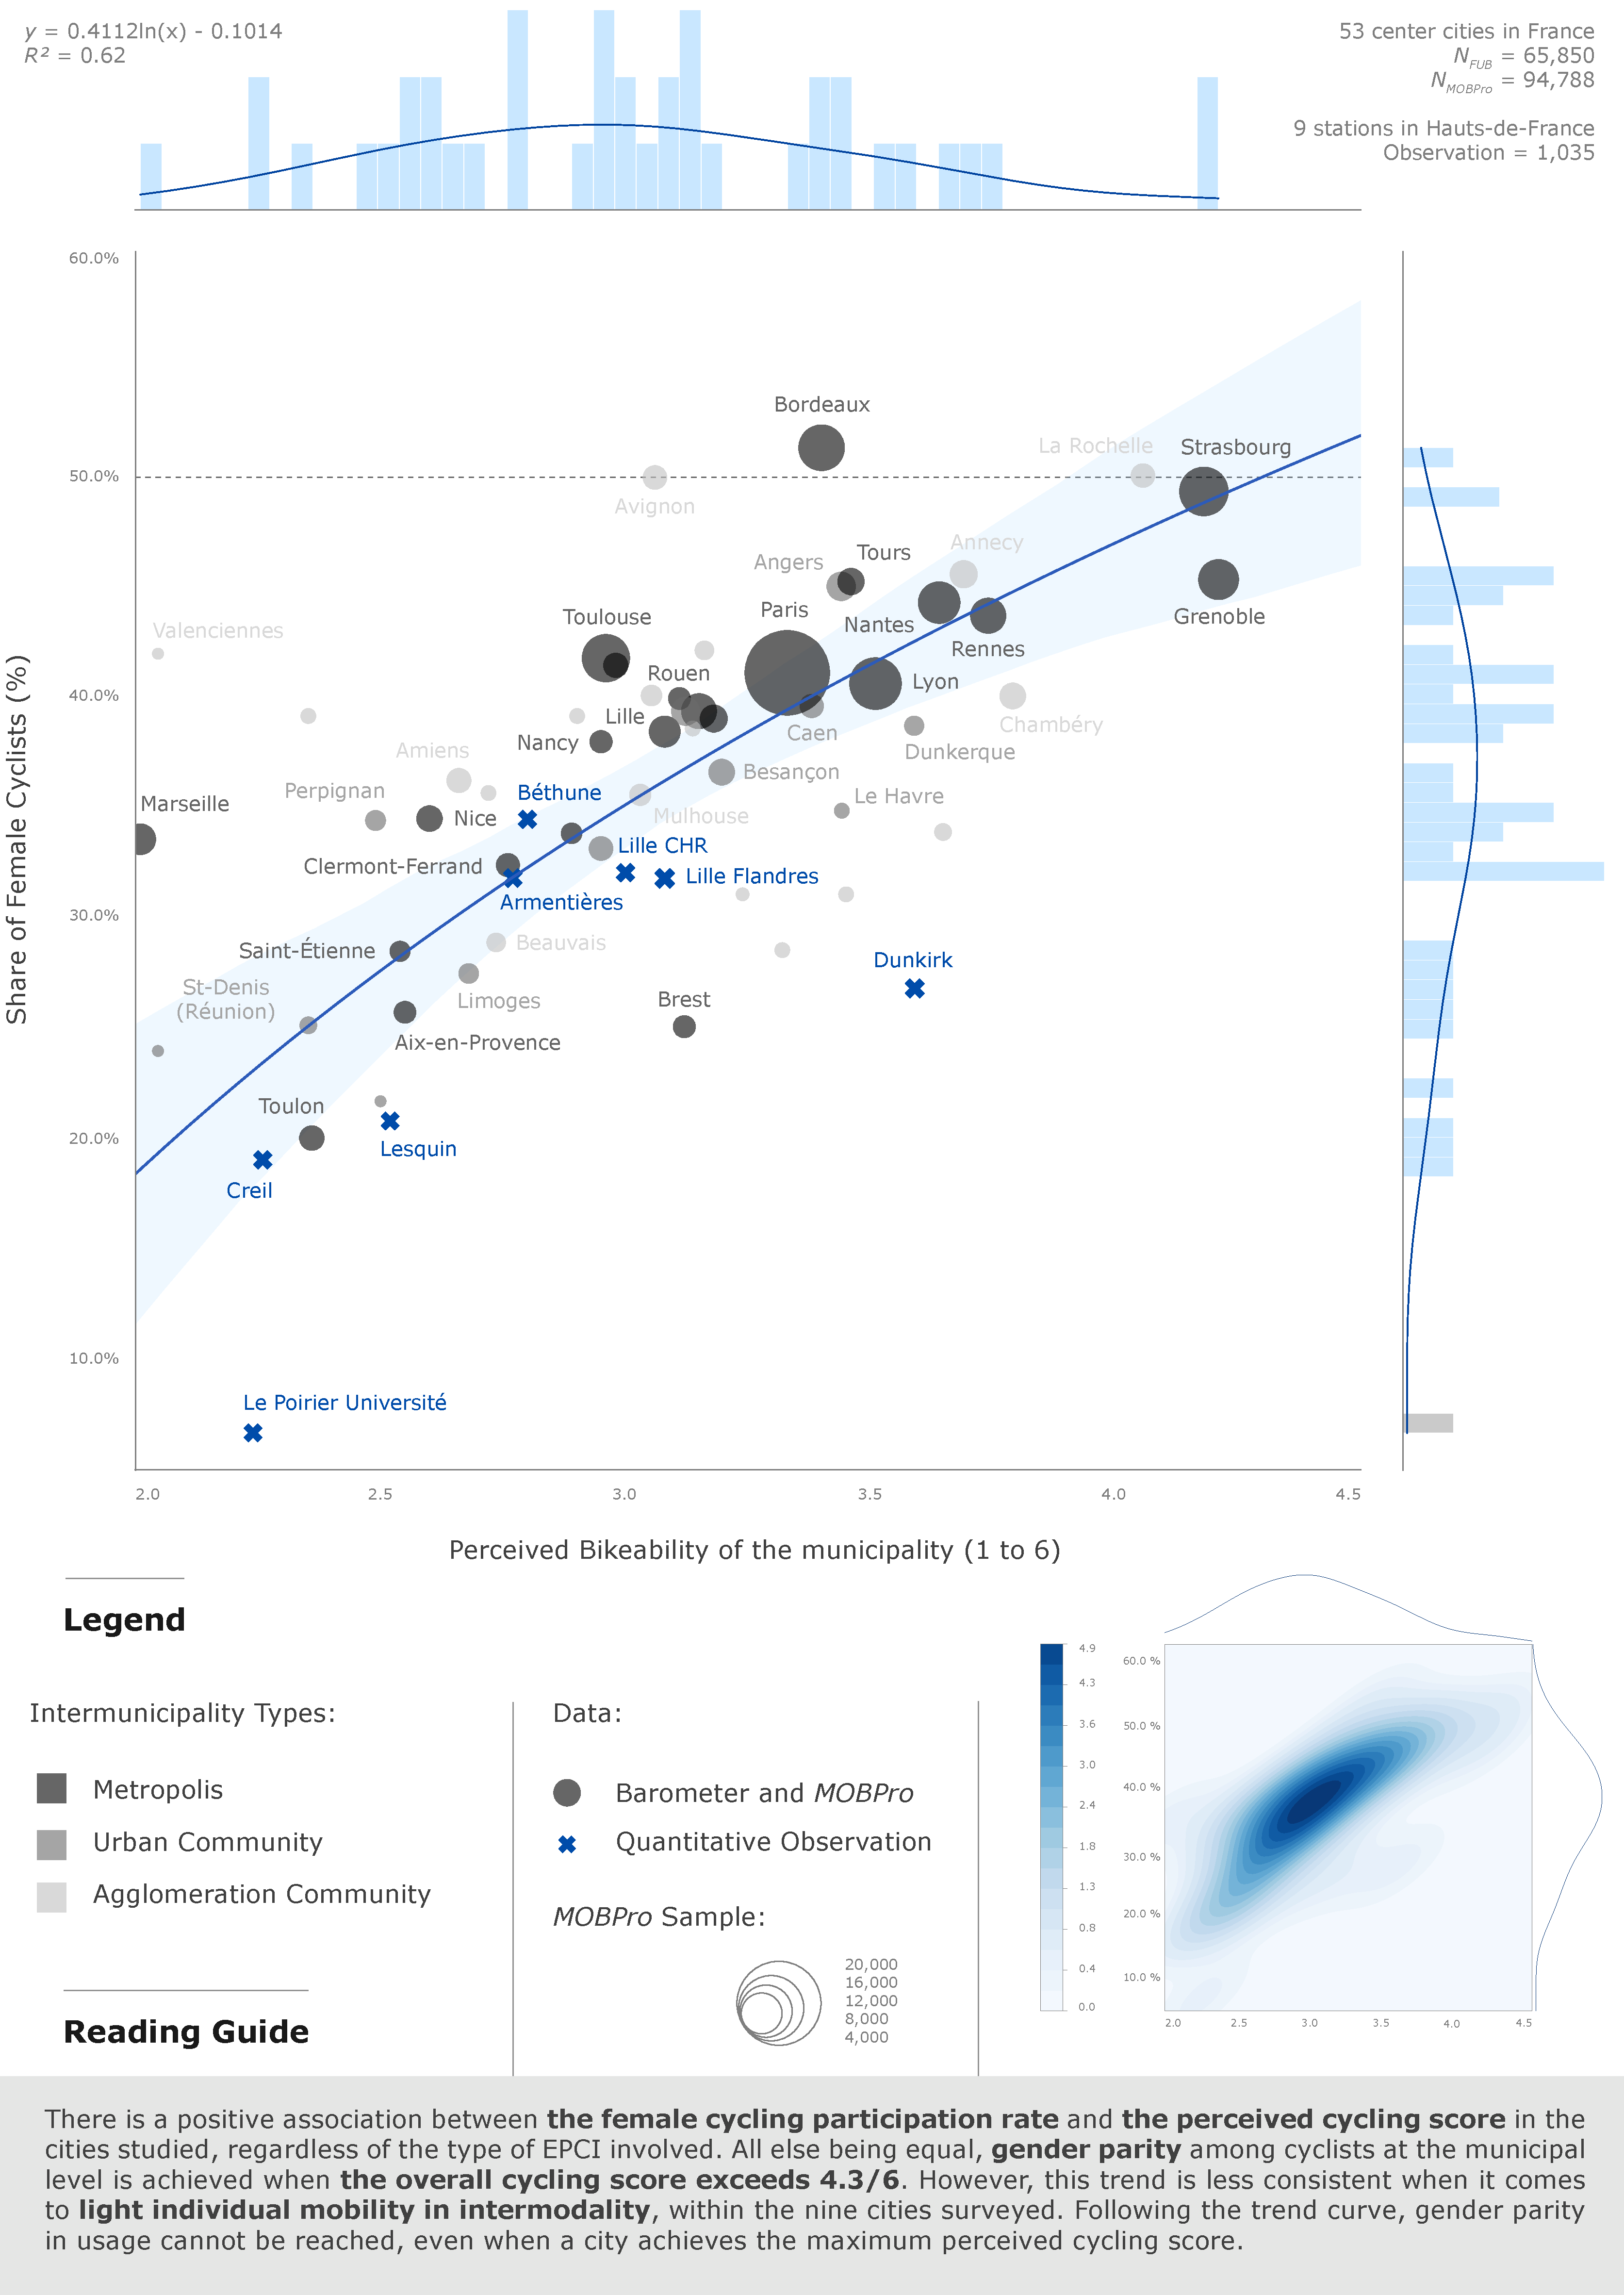
\includegraphics[width=1\columnwidth]{src/Figures/Chap-4/EN_Regression_genre_cyclabilite_OLS.pdf}}
    \vspace{5pt}
    \begin{flushright}\scriptsize{
    Datasets: \textsl{Barometer of Cyclable Cities} \textcolor{blue}{\autocite{fub_barometre_2021}} and \textsl{MOBPro} \textcolor{blue}{\autocite{insee_documentation_2023}}
    \\
    Author: \textcolor{blue}{Dylan Moinse (2023)}
    %\\
    %Created with \Marque{Python}~and \Marque{Illustrator}
    }\end{flushright}
\end{figure}

%% Linear regression - Quantitative observation
Taking into account the quantitative observation of intermodal travelers opting for bicycles or micromobility solutions in the region, this statistical analysis supports the linear regression curve exploring the gendered use of bicycles in relation to bikeability, particularly regarding \acrshort{PeS} when associated with the train. By way of illustration, consider the case of users relying on electric scooters at the Poirier Université stop, who are very rarely women (5\%, from 19 observations) and face a bikeability score of 2.24. This trend is also reflected at the Lesquin stations (16\%, from 19 observations), Armentières (17\%, from 58 observations), and Creil (19\%, from 54 observations), where the bikeability scores range from 2.26 to 2.77. \textsl{In contrast}, gender-related disparities are less pronounced at the Lille Flandres stations (28\%, from 127 observations), Béthune (31\%, from 35 observations), and Lille CHR (32\%, from 57 observations), where the perceived bikeability is between 2.80 and 3.08.%%Translated%%

%% Dunkirk exception
However, the Dunkirk station is an exception, characterized by relatively high bikeability but still dominated by male users for cycling and micromobility (29\%, from 91 observations). This phenomenon may be linked to the effects of the free public transport policies introduced in 2018 \textcolor{blue}{\autocite{heran_transports_2020}}\index{Héran, Frédéric|pagebf}, whose gendered impact remains to be studied\footnote{~
    More generally, discussions continue to fuel the scientific and operational community regarding the relationship between free public transport policies and bicycle use. In Dunkirk, \textcolor{blue}{Claire-Marine} \textcolor{blue}{\textcite[89]{javary_gratuite_2020}}\index{Javary, Claire-Marine|pagebf}\index{Delevoye, Vanessa|pagebf}\index{Hasiak, Sophie|pagebf}\index{Huré, Maxime|pagebf} suggests that there is no modal substitution effect between bicycles and proposes moving beyond this debate to envision an intermodal system positioning these modes of transport as allies in the mobility transition.
}. In comparison to the exclusive use of conventional bicycles, a second emerging result is the reduced representation of women among intermodal micromobility users within the same city (see \hyperref[fig-chap4:regression-genre-cyclabilite]{Figure~\ref{fig-chap4:regression-genre-cyclabilite}}, page~\pageref{fig-chap4:regression-genre-cyclabilite}). This observation highlights that a bikeability score of 4.3/6 would not be sufficient to achieve gender parity among rail passengers opting for light individual mobility. In fact, a score higher than the maximum possible value, which is six points, would be required for the curve to reach a parity threshold. This trend thus suggests that improving the bikeability of territories alone would not be enough to address the gender inequalities observed regarding intermodal micromobility use.%%Translated%%

%% Linear regression figure for bikeability and gender
\begin{figure}[h!]\vspace*{4pt}
    \caption{Linear regression model between the gender distribution of bicycles and the factors used to aggregate the perceived bikeability score.}
    \label{fig-chap4:regression-genre-cyclabilite-questions-detailees}
    \centerline{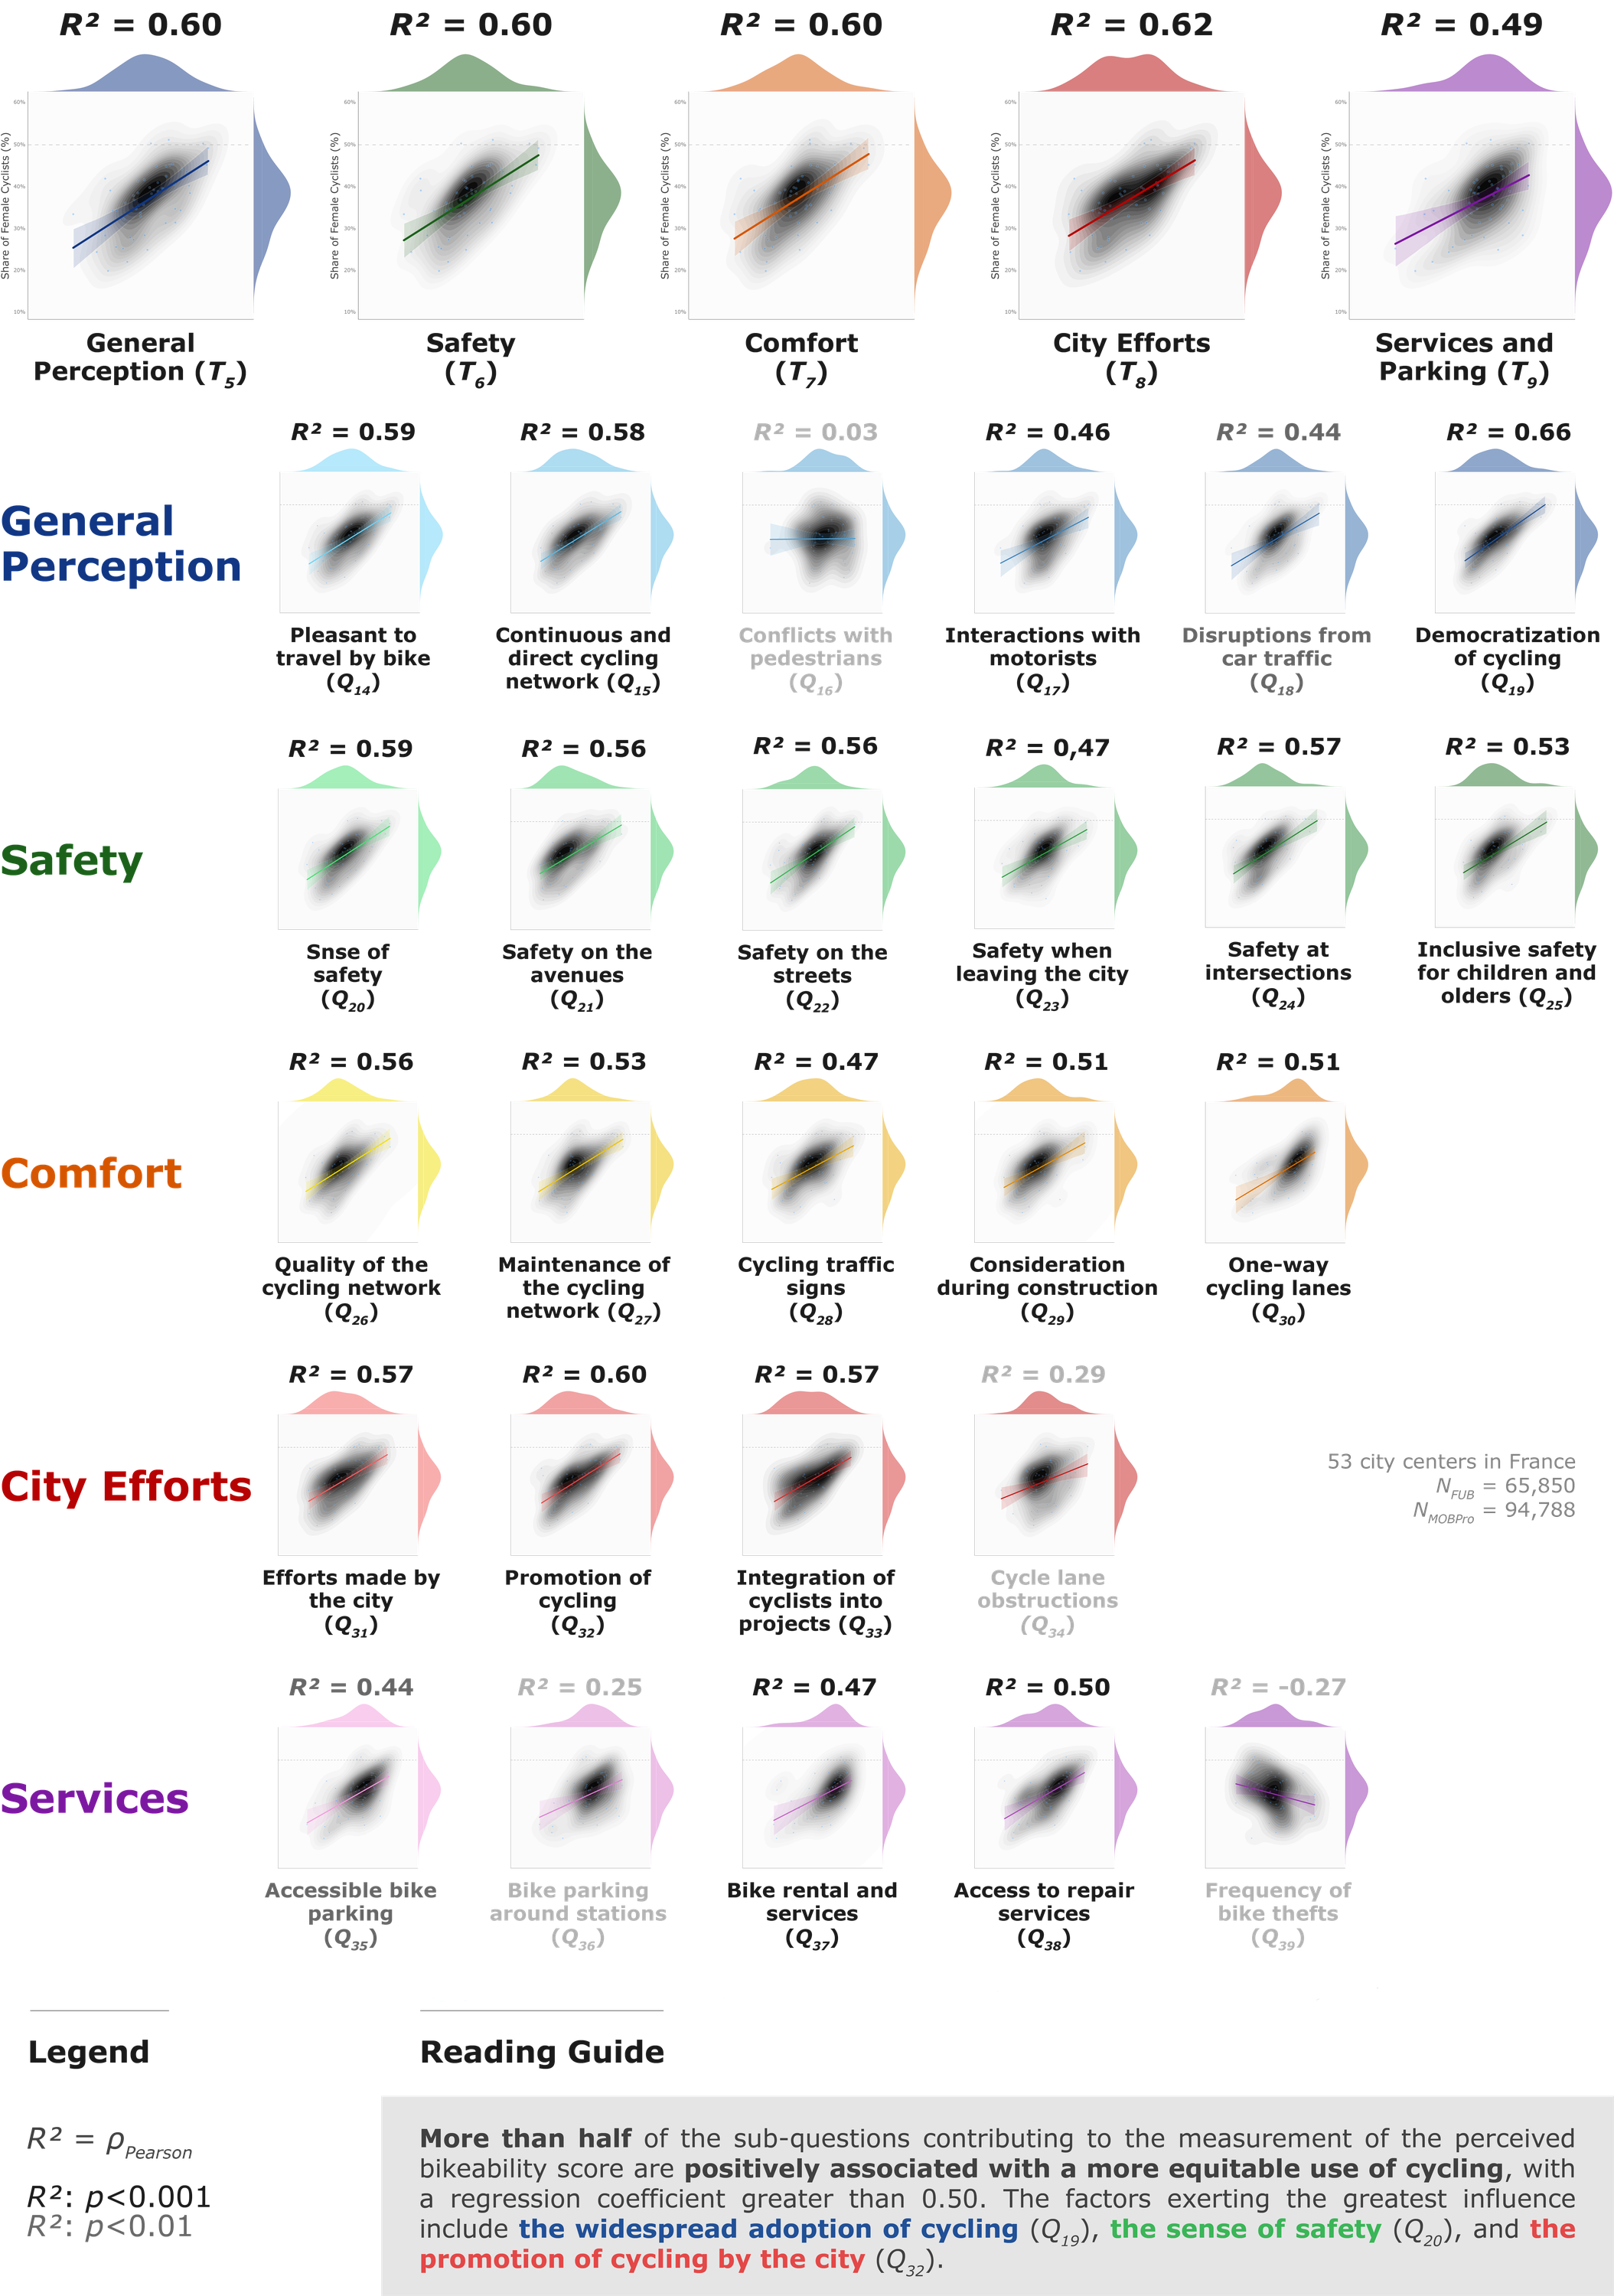
\includegraphics[width=1\columnwidth]{src/Figures/Chap-4/EN_Regression_sous_facteurs_OLS.png}}
    \vspace{5pt}
    \begin{flushright}\scriptsize{
    Datasets: \textsl{Barometer of Cyclable Cities} \textcolor{blue}{\autocite{fub_barometre_2021}} and \textsl{MOBPro} \textcolor{blue}{\autocite{insee_documentation_2023}}
    \\
    Author: \textcolor{blue}{Dylan Moinse (2023)}
    }\end{flushright}
\end{figure}

%% Categories related to bikeability
Once the link was established between the issues related to perceived bikeability and the unequal use of light individual mobility through the lens of gender, the statistical analysis was refined to discern the sub-factors exerting a certain weight in this positive association. The goal of this investigation is to offer a qualitative perspective on bikeability. By re-examining the five themes defined in the context of the questionnaire conducted by \textcolor{blue}{\textcite{fub_barometre_2021}}\index{FUB@\textsl{FUB}|pagebf}, it is possible to determine the influence of each dimension evaluated by bicycle users, while maintaining the interrelations between bikeability and the gender representation of cyclists. The first theme of the questionnaire, focusing on the \textsl{general perception} (\(T_{5}\)) of the cycling environment, shows a significantly positive association with the gendered use of bicycles ($\hat{\beta}_{5}$~=~0.96,~$p$\textless0.06), revealing a much stronger influence than that of the presence of cycling infrastructure or the promotion of cycling in urban areas. Moreover, the score for \textsl{city efforts} (\(T_{8}\)) significantly contributes to promoting more equitable use of bicycles ($\hat{\beta}_{8}$~=~0.58,~$p$\textless0.05). In contrast, the indicator related to \textsl{comfort} (\(T_{7}\)) on bicycles shows a negative association ($\hat{\beta}_{7}$~=~-0.65,~$p$\textless0.08). In contrast, the themes related to \textsl{security} (\(T_{6}\)) and \textsl{services and parking} (\(T_{9}\)) do not show any significant association ($\hat{\beta}_{6}$~=~-0.75 and $\hat{\beta}_{9}$~=~-0.22,~$p$~\texttt{>}~0.10). Similarly, regarding the sub-questions included in the questionnaire on perceived bikeability in France, no significant association was derived from the multivariate regression.%%Translated%%

%% Influence
The results of the \acrshort{OLS} regression provide insight into the relationships between various independent indicators and the gendered use of bicycles at the national level. The data being normalized, the standard deviation serves as the unit of measurement. Therefore, the coefficients $\hat{\beta}_{i}$ indicate the extent to which female participation in cycling fluctuates in response to variations in each independent indicator, all else being equal:
\begin{customitemize}
    \item An increase of one standard deviation in the \textsl{general perception} score (\(T_{5}\), perceived bikeability) is associated with an increase of 0.959 times the standard deviation of the dependent variable;
    \item An increase of one standard deviation in the proportion of cycling routes on the road network (\(T_{3}\), objective bikeability) is associated with an increase of 0.595 times the standard deviation of the dependent variable;
    \item An increase of one standard deviation in the \textsl{city efforts} score (\(T_{8}\), perceived bikeability) is associated with an increase of 0.578 times the standard deviation of the dependent variable;
    \item An increase of one standard deviation in the modal share of cycling (\(T_{1}\), safety by numbers) is associated with an increase of 0.368 times the standard deviation of the dependent variable.
\end{customitemize}%%Translated%%

%% Sub-questions on bikeability
By studying each question in detail, a series of \textsl{Pearson} linear regressions \textcolor{blue}{\autocite{pearson_vii_1896}}\index{Pearson, Karl|pagebf}\index{Henrici, Olaus Magnus Friedrich Erdmann|pagebf} reveals a relatively significant correlation overall, with a coefficient of determination ($R^2$) exceeding 0.50 for more than half of the questions, as demonstrated by \hyperref[fig-chap4:regression-genre-cyclabilite-questions-detailees]{Figure~\ref{fig-chap4:regression-genre-cyclabilite-questions-detailees}} (page~\pageref{fig-chap4:regression-genre-cyclabilite-questions-detailees}). The following factors, in particular, exert a substantial influence:
    \begin{customitemize}
\item The widespread adoption of bicycles (\(Q_{19}\),~$R^2$~=~0.66);
\item The feeling of safety while cycling (\(Q_{20}\),~$R^2$~=~0.60);
\item The feeling of safety when cycling through residential streets (\(Q_{22}\),~$R^2$~=~0.60);
\item The promotion of cycling by the city (\(Q_{32}\),~$R^2$~=~0.60);
\item The fun and pleasant aspect of cycling in the city (\(Q_{14}\),~$R^2$~=~0.59);
\item The ability to move quickly and directly through the cycling network (\(Q_{15}\),~$R^2$~=~0.58);
\item The safety experience when crossing intersections (\(Q_{24}\),~$R^2$~=~0.57);
\item The involvement of cyclists in mobility and urban development projects (\(Q_{33}\),~$R^2$~=~0.57);
\item Municipal efforts to strengthen bicycle development (\(Q_{31}\),~$R^2$~=~0.57);
\item The quality of the cycling network (\(Q_{26}\),~$R^2$~=~0.56);
\item The feeling of safety on major roads (\(Q_{21}\),~$R^2$~=~0.56).
    \end{customitemize}
Only two questions do not contribute to the relationship between bikeability and the gender distribution of bicycles: those related to conflicts with pedestrians (\(Q_{16}\),~$R^2$~=~0.03) and the frequency of bicycle thefts (\(Q_{39}\),~$R^2$~=~-0.27).%%Translated%%

%% Synthesis of sub-questions
It appears that multiple factors play a crucial role in the concept of bikeability as an explanatory variable for a more inclusive development of light individual mobility in France. The democratization of cycling, coupled with its visibility, emerges as a key sub-variable in this equation, along with considerations regarding cyclists' sense of safety, the establishment of a continuous and direct cycling network in residential areas, and the implementation of two-way cycling streets, all of which play a fundamental role in promoting a positive experience. Furthermore, cycling policies driven by the city are of equal importance alongside effective communication strategies and urban project consultations involving cyclists. In parallel, it is essential not to underestimate the factors contributing to the improvement of bikeability within municipalities, notably the sense of safety on major roads, at intersections and roundabouts, the development of secure infrastructure tailored to the needs of the most vulnerable populations, the maintenance of the cycling network, and convenient access to bicycle repair services (see \hyperref[fig-chap4:regression-genre-cyclabilite-questions-detailees]{Figure~\ref{fig-chap4:regression-genre-cyclabilite-questions-detailees}}, page~\pageref{fig-chap4:regression-genre-cyclabilite-questions-detailees}).%%Translated%%

%% Commented Routes 1
In this section, we surveyed the perception of various elements that influence the quality of bikeability in the territories. The testimony of participant \(PCTE_{1}\) provides a rich and detailed insight into these aspects. She shares her vision of an urban environment in which \Commas{\textsl{the aspect} [related to] \textsl{security with bike lanes and cycle tracks} [and] \textsl{the pleasant city as well} [\dots] \textsl{a calm city, without too many cars}} [20:17, \(PCTE^{TC}_{1}\)] are prioritized factors. The \textsl{feeling of safety} (\(Q_{20}\)) is addressed by the participant, who mentions the \textsl{interactions} (\(Q_{17}\)) and \textsl{inconveniences} (\(Q_{18}\)) related to automobile traffic in terms of volume and speed, stating that \Commas{\textsl{with the sloping road, cars go much faster than} [her] \textsl{scooter\dots~And} [she does not feel] \textsl{safe on this part of the path. We are mixed with them, and [she finds herself] stuck between the cars that are moving and those that are parked.}} [\(PCTE^{A}_{1}\)]. These vulnerability situations generate a feeling of discomfort and helplessness, degrading the \textsl{pleasure} of moving by bike or micromobility (\(Q_{14}\)), as the participant explains: \Commas{\textsl{which is, not stressful, but let’s say\dots a bit more annoying} [\dots] \textsl{there are \textsl{many} cars, and since my scooter only goes up to 25 km/h, I am afraid of bothering the cars. So, I position myself at the side of the road and try to speed up as much as possible.}} [00:27, \(PCTE^{TC}_{1}\)].%%Translated%%

%% Figure 2 PCTE1E Maubeuge
\begin{figure}[h!]\vspace*{4pt}
    \caption{Image extracted from the filmed route leading to the Lille Flandres station, illustrating the maneuver to avoid obstructive parking (\(PCTE^{A}_{1}\)).}
    \label{fig-chap4:pcte1a-stationnement-genant}
    \centerline{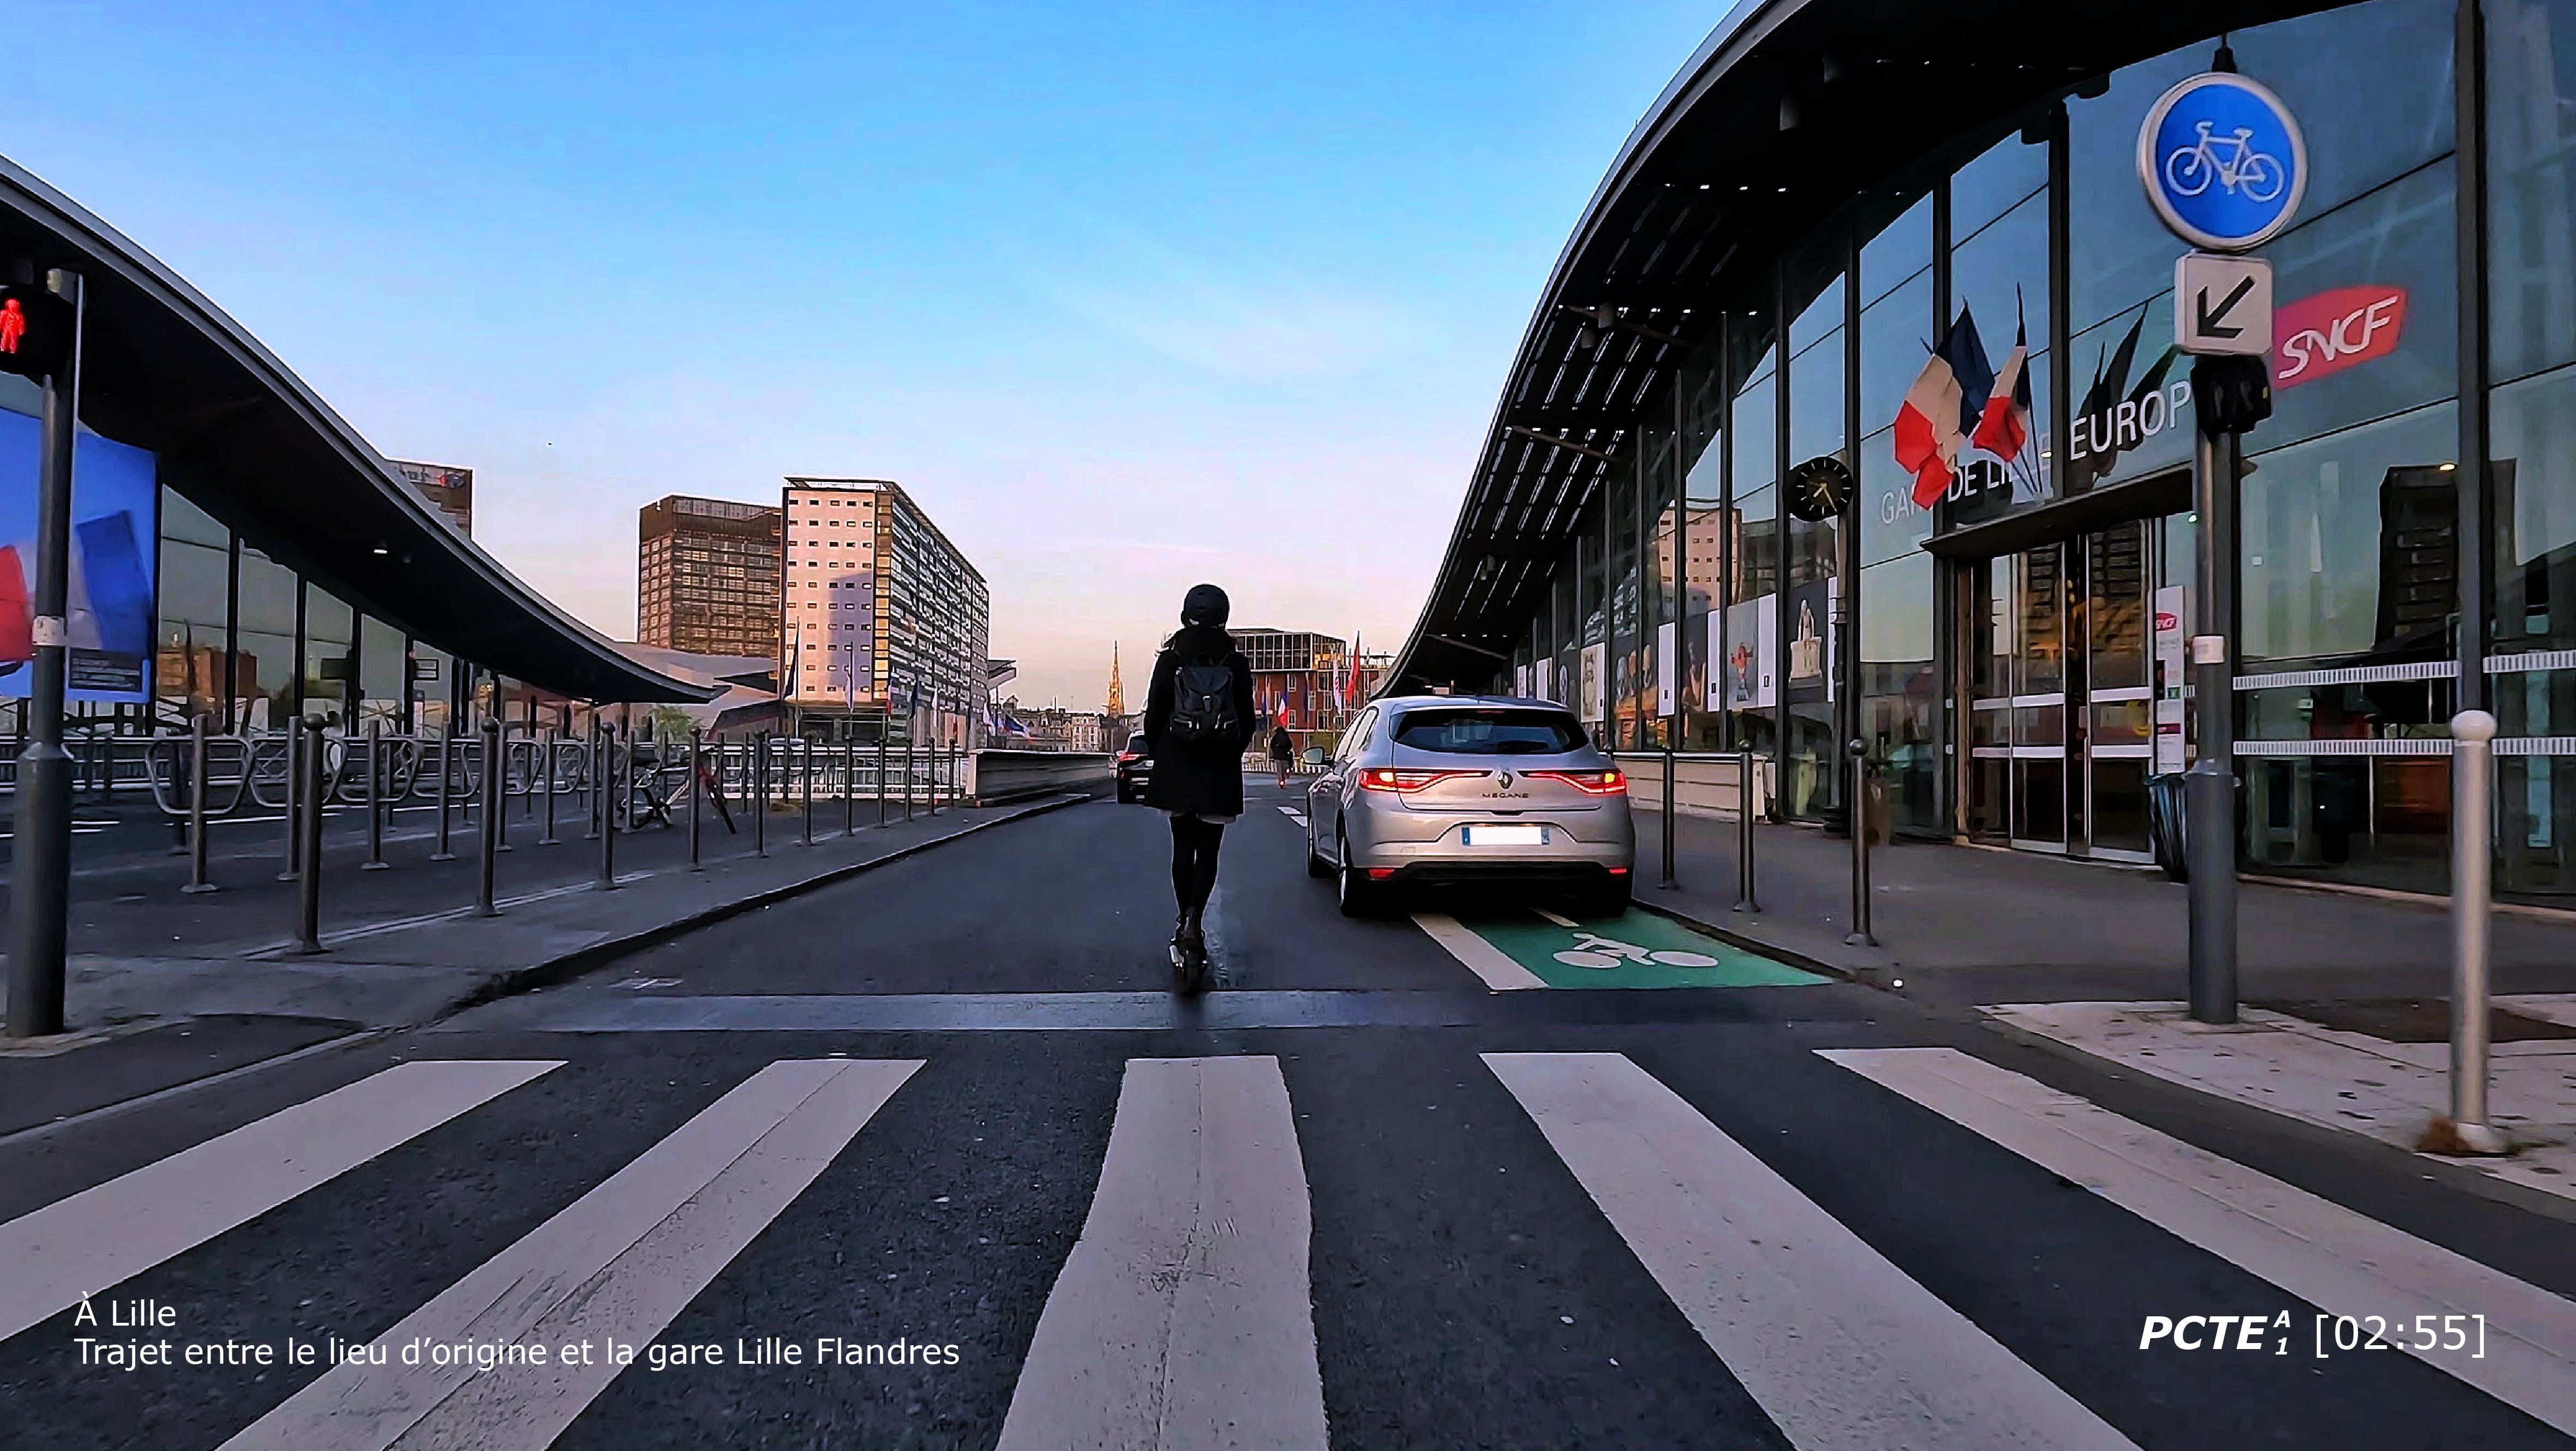
\includegraphics[width=1\columnwidth]{src/Figures/Chap-4/Extrait_Video_PCTE1_Access_8.jpg}}
    \vspace{5pt}
    \begin{flushright}\scriptsize{
    Author: \textcolor{blue}{Dylan Moinse (2022)}
    }\end{flushright}
\end{figure}

%% Commented Routes 2
Intersection management is also a critical point, much more described by the participant from \(PCTE_{1}\) than the participant from \(PCTE_{2}\). The treatment of \textsl{intersections} (\(Q_{24}\)) arises in the difficulties encountered in cycling practice, as in the \Commas{\textsl{big black spot} [which] \textsl{is the roundabout} [\dots] [where the participant has] \textsl{fear when} [she is] \textsl{in the roundabout, because} [she cannot] \textsl{turn too much} [to] \textsl{see what’s happening behind her since} [she is] \textsl{less stable on a scooter than on a bike}.} [03:04, \(PCTE^{TC}_{1}\)]. Furthermore, the \textsl{quality of the cycling network} (\(Q_{26}\)) is a determining factor for secure movement in light individual mobility. The participant expresses a preference for bus-only lanes, which she finds \Commas{\textsl{pleasant}}, as she can \Commas{\textsl{move quite easily}} [00:27, \(PCTE^{TC}_{1}\)] and \Commas{\textsl{because it’s much safer, as it’s wider}} [02:16, \(PCTE^{TC}_{1}\)], both in Lille and Maubeuge. However, she addresses bike lanes with less enthusiasm, mentioning situations where she feels forced to avoid certain sections due to the inattention of motorists, being \Commas{\textsl{on the side}} [00:27, \(PCTE^{TC}_{1}\)], while \Commas{\textsl{cars don’t pay attention}} [03:04, \(PCTE^{TC}_{1}\)] (see \hyperref[fig-chap4:pcte1a-stationnement-genant]{video excerpt~\ref{fig-chap4:pcte1a-stationnement-genant}}, page~\pageref{fig-chap4:pcte1a-stationnement-genant}). Finally, the commented route conducted with the user in \acrshort{PeS} provides a final insight into the importance of \textsl{signage} (\(Q_{28}\)) and \textsl{communication and promotion of cycling} (\(Q_{32}\)) by public authorities. A well-designed and clearly indicated cycling network is essential to avoid confusion and usage conflicts between cyclists and motorists. The participant points out the gaps in these areas, notably the lack of visibility and clear information, with the network \Commas{[lacking] \textsl{colors} [\dots] \textsl{and information}.} [\(PCTE^{E}_{1}\)] (see \hyperref[fig-chap4:pcte1e-voie-bus]{video excerpt~\ref{fig-chap4:pcte1e-voie-bus}}, page~\pageref{fig-chap4:pcte1e-voie-bus}).%%Translated%%

%% Figure 3 PCTE1E Maubeuge
\begin{figure}[h!]\vspace*{4pt}
    \caption{Image extracted from the filmed route broadcasted from the Maubeuge station, revealing a bus lane lacking discernible ground markings (\(PCTE^{E}_{1}\)).}
    \label{fig-chap4:pcte1e-voie-bus}
    \centerline{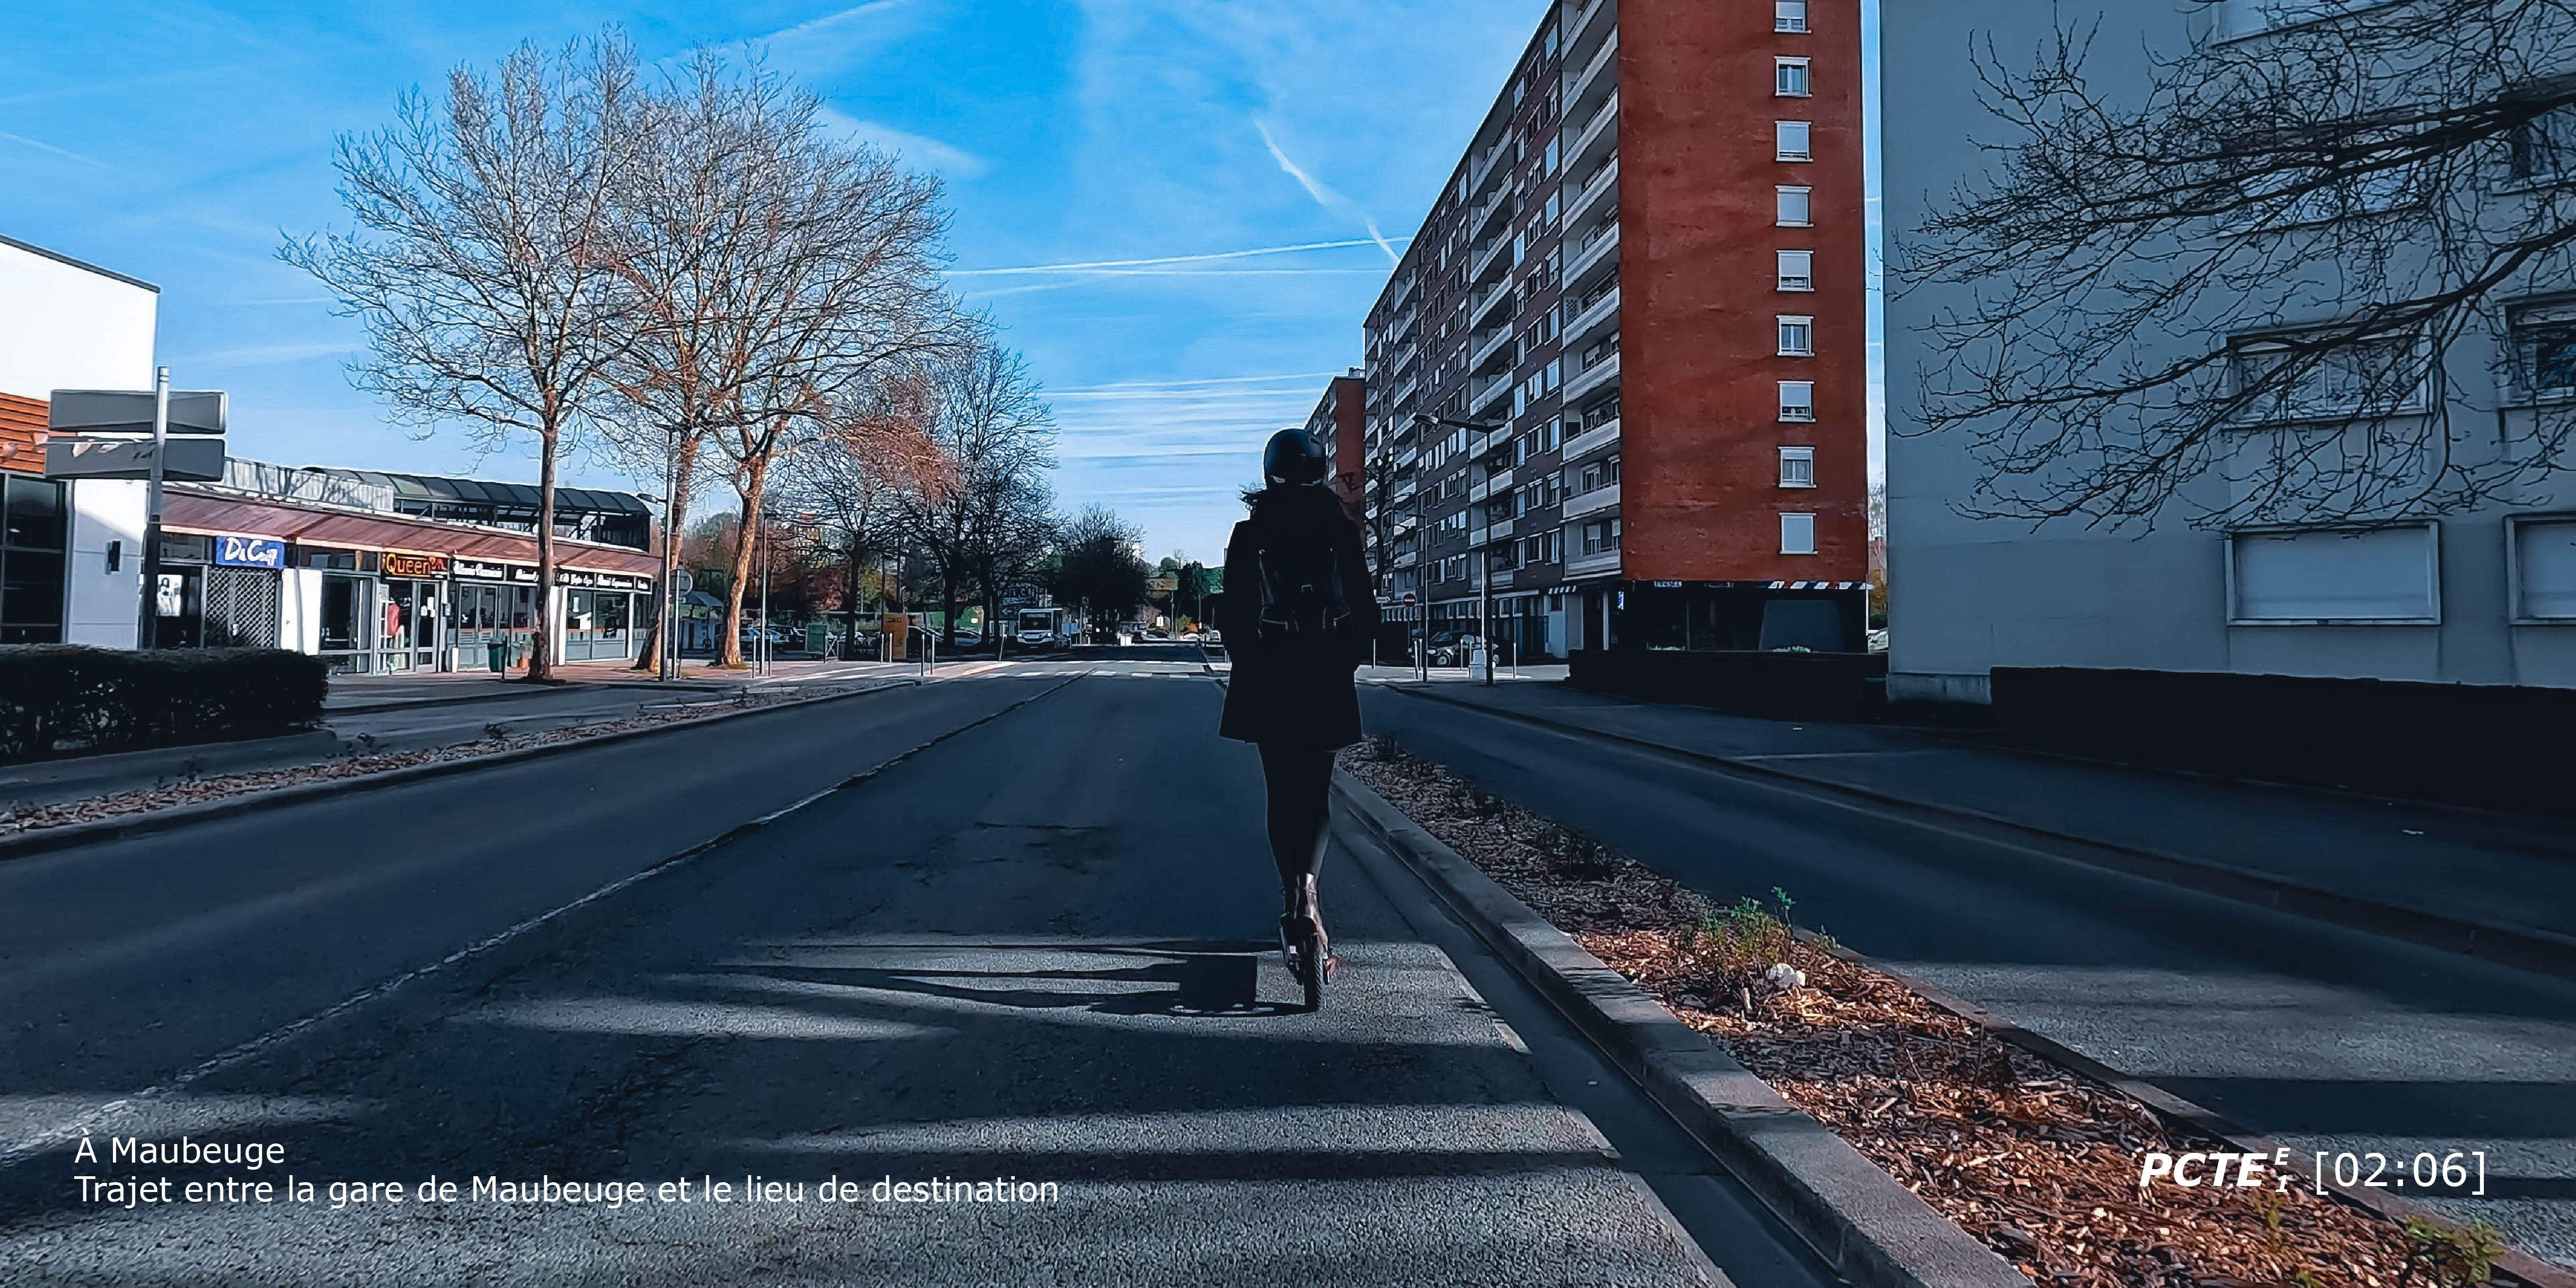
\includegraphics[width=1\columnwidth]{src/Figures/Chap-4/Extrait_Video_PCTE1_Egress_4.jpg}}
    \vspace{5pt}
    \begin{flushright}\scriptsize{
    Author: \textcolor{blue}{Dylan Moinse (2022)}
    }\end{flushright}
\end{figure}

% 4.3.3.4.
\needspace{1\baselineskip} % Reserve space
\subsubsection*{Photographing the French Cities Surveyed According to the Gender Distribution of Cyclists
    \label{chap4:comparaison-villes-fr-genre}
    }

    %% City Ranking
Through a quantitative analysis of the datasets provided by \textcolor{blue}{\textcite{fub_barometre_2021}}\index{FUB@\textsl{FUB}|pagebf} and \textcolor{blue}{\textcite{insee_documentation_2023}}\index{Insee@\textsl{Insee}|pagebf}, this sub-section aims to classify the 53 French cities based on their bikeability ratings and the degree of feminization in cycling practice. To do so, the research employed a bivariate analysis\footnote{~
    A bivariate analysis is a statistical method that examines the relationship between two variables, characterizing how they interact. It helps to understand whether there is a correlation or dependence between these two variables, as well as the nature of this relationship, whether positive or negative. A bivariate analysis can result in the production of a graphical representation, such as a bivariate map. This type of mapping highlights the two variables jointly, aiming to visually show how they behave in relation to each other.
} to highlight the positive correlation observed geographically. Four categories emerge from this statistical analysis: (i) cities tending towards gender parity and supportive of cycling development; (ii) cities supportive of cycling development but showing gender inequalities; (iii) cities tending towards gender parity but unfavorable to cycling development; and (iv) cities showing gender inequalities and unfavorable to cycling (see \hyperref[fig-chap4:carte-bivariee-genre-cyclabilite]{Map~\ref{fig-chap4:carte-bivariee-genre-cyclabilite}}, page~\pageref{fig-chap4:carte-bivariee-genre-cyclabilite}).%%Translated%%

%% Bivariate Map of Bikeability and Gendered Use
\begin{carte}[h!]\vspace*{4pt}
    \caption{Bivariate map of the 53 French cities examined based on the gender distribution of cycling and perceived bikeability.}
    \label{fig-chap4:carte-bivariee-genre-cyclabilite}
    \centerline{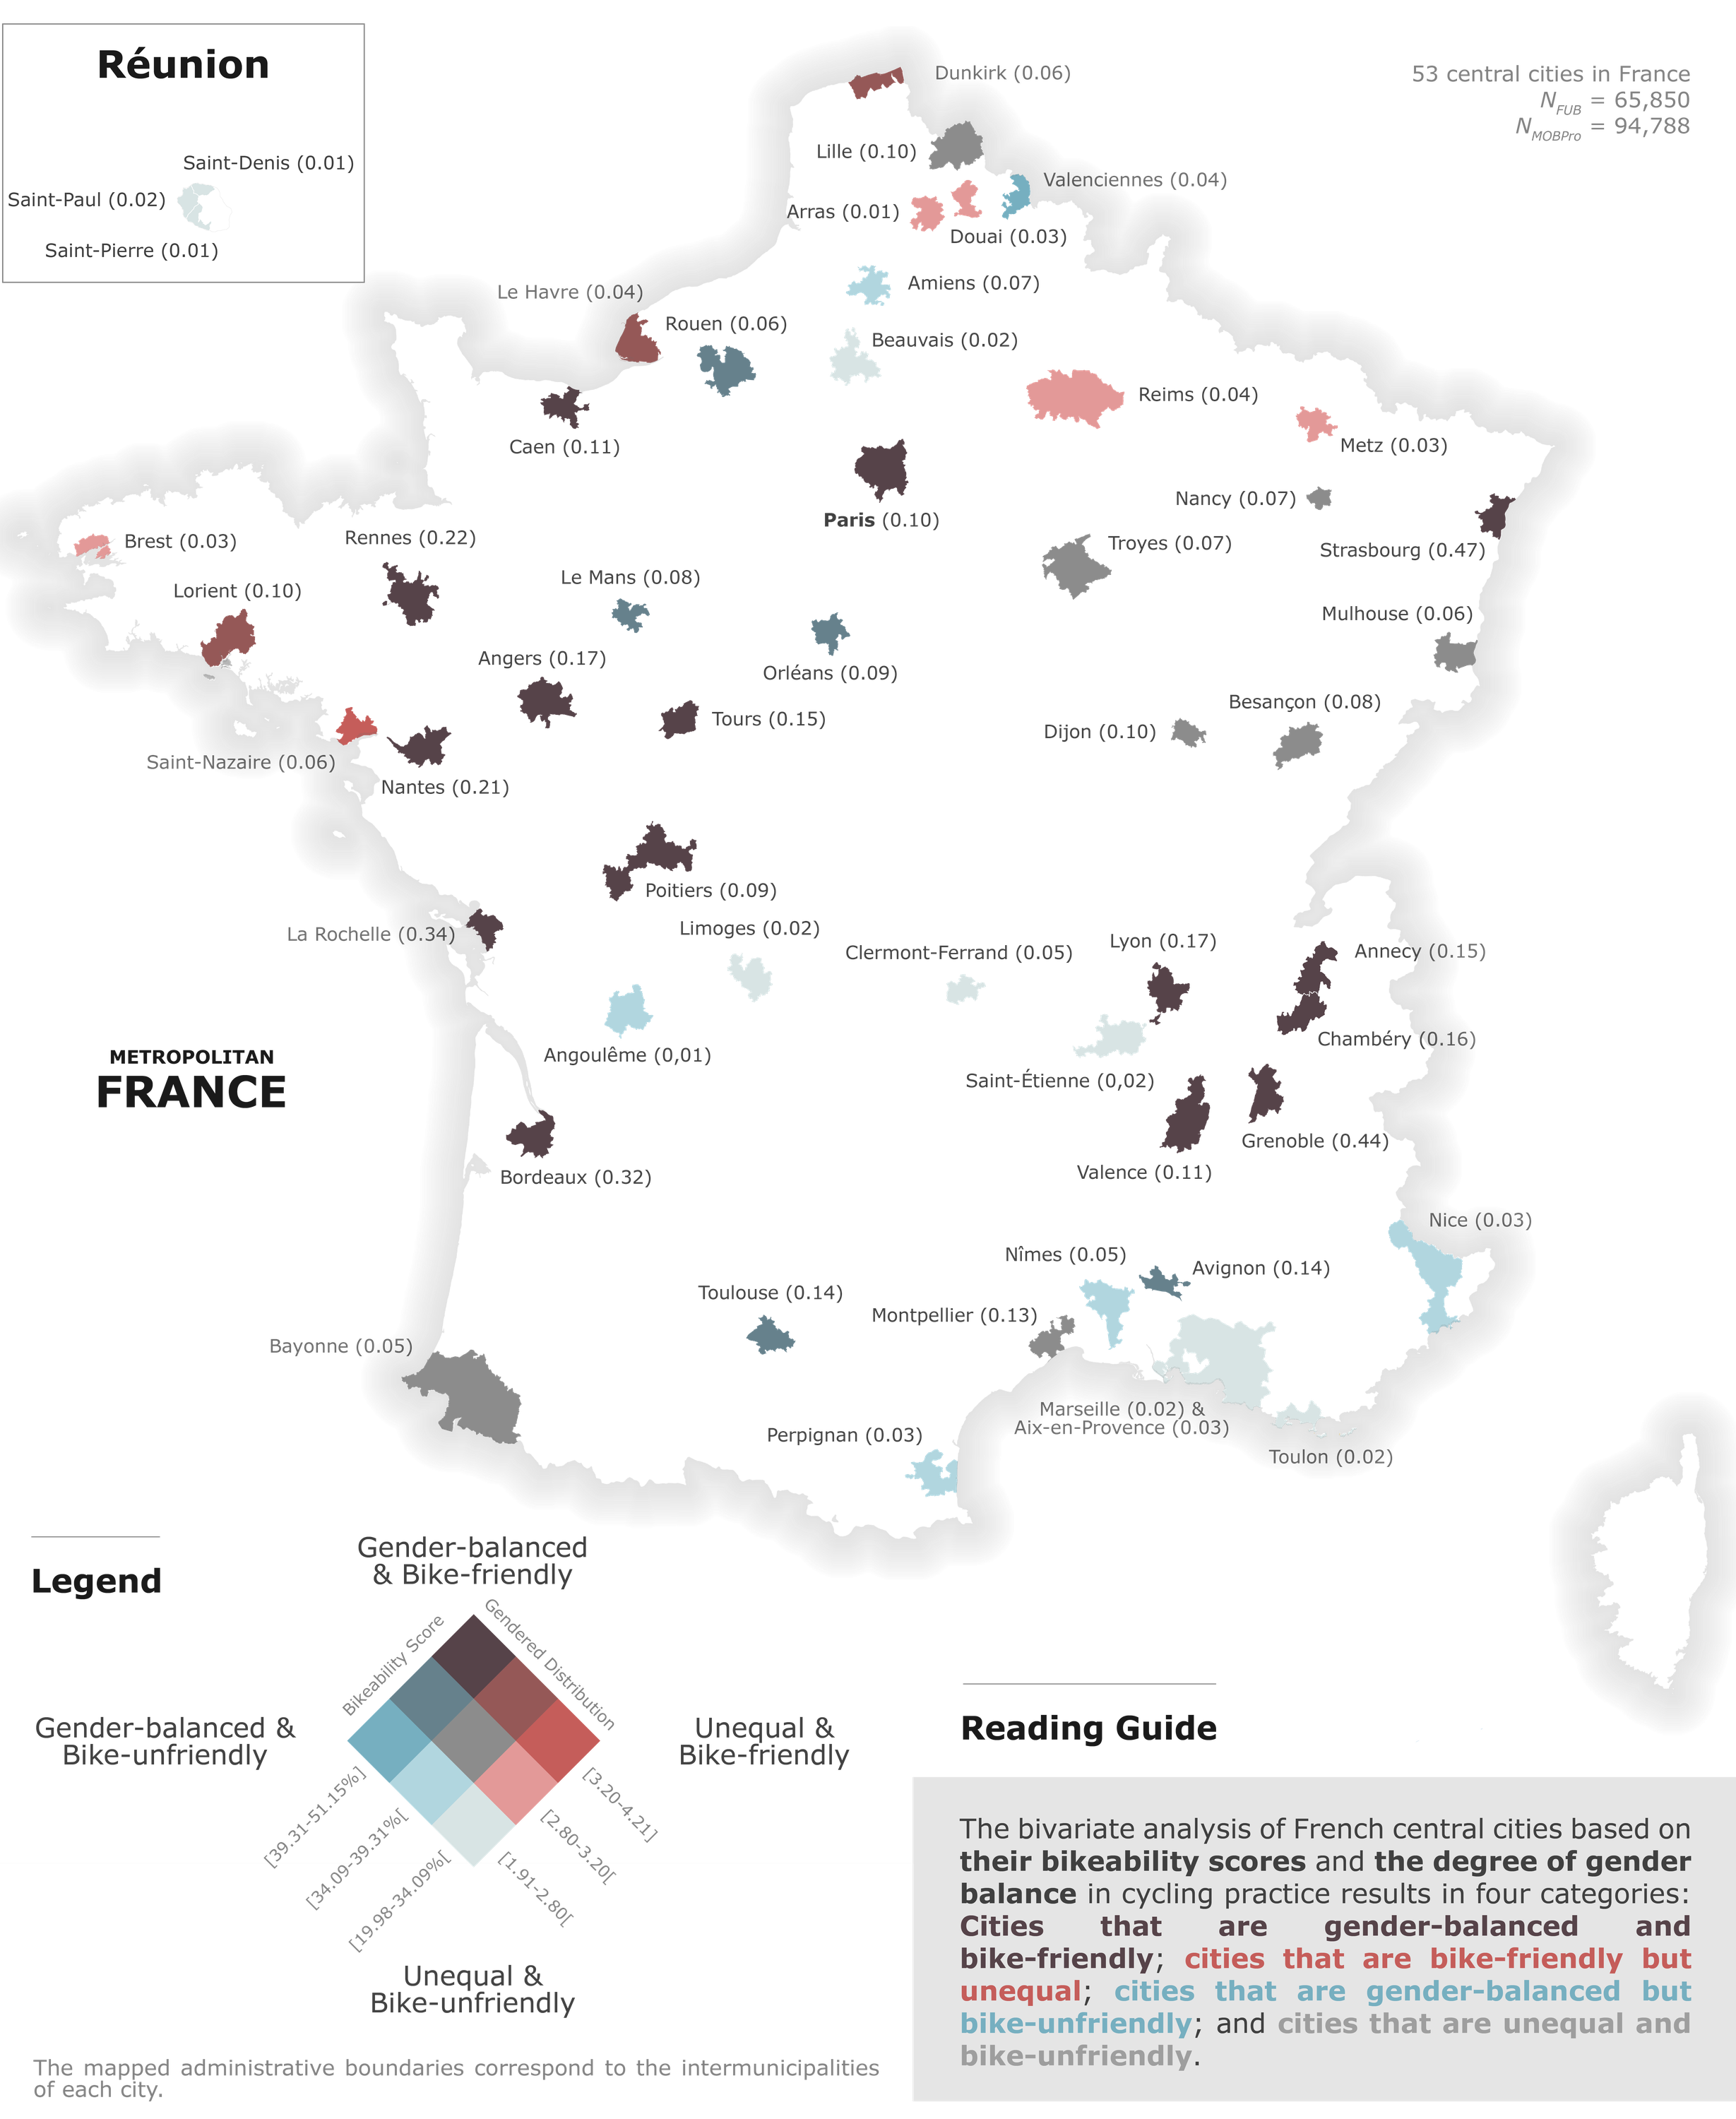
\includegraphics[width=1\columnwidth]{src/Figures/Chap-4/EN_Carte_bivariee_cyclabilite_genre_OLS.png}}
    \vspace{5pt}
    \begin{flushright}\scriptsize{
    Datasets: \textsl{Barometer of Cyclable Cities} \textcolor{blue}{\autocite{fub_barometre_2021}} and \textsl{MOBPro} \textcolor{blue}{\autocite{insee_documentation_2023}}
    \\
    Author: \textcolor{blue}{Dylan Moinse (2023)}
    }\end{flushright}
\end{carte}

%% Description of the Extremes Map
The \hyperref[fig-chap4:carte-bivariee-genre-cyclabilite]{Map~\ref{fig-chap4:carte-bivariee-genre-cyclabilite}} (page~\pageref{fig-chap4:carte-bivariee-genre-cyclabilite}) provides a visual representation placing cities based on the gender distribution of cycling and the perceived bikeability by users, using regular intervals. The typology of the fifty-three cities studied highlights those characterized by gender-equal cycling use and high bikeability scores. These cities are primarily located in the west of metropolitan France, except for Brittany, including Bordeaux, Nantes, Rennes, Tours, Angers, Poitiers, as well as cities in the east of the country, such as Strasbourg, Grenoble, Annecy, Chambéry, and Lyon. In contrast, cities receiving lower evaluations for both variables are mainly situated in the south of metropolitan France, encompassing places such as Toulon, Marseille, Aix-en-Provence, Saint-Étienne, Limoges, and Clermont-Ferrand. This also applies to cities in the department of Réunion, such as Saint-Pierre, Saint-Paul, and Saint-Denis, which fall into this category.%%Translated%%

%% Description of the Nuances Map
Furthermore, several regions that offer favorable conditions for cycling but face challenges in achieving a balanced gender distribution of cycling are primarily located in the north of metropolitan France, including cities such as Dunkirk, Le Havre, Arras, Douai, and Reims, as well as in Brittany, with examples such as Lorient, Brest, and Saint-Nazaire. In contrast, some cities exhibit a relatively balanced gender distribution of cycling but still maintain relatively low bikeability levels. This latter category is illustrated by cities such as Amiens, Angoulême, Nice, Nîmes, and Valenciennes.%%Translated%%

% 4.3.3.5.
\needspace{1\baselineskip} % Reserve space
\subsubsection*{Definition of an Indicator Based on the Inclusive Development of Cycling and Bikeability
    \label{chap4:definition-indicateur-genre}
    }

    %% Indicator
Based on the three variables examined throughout this sub-section, namely the gender distribution of cyclists, the modal share of cycling, and the bikeability score of a municipality, the final objective of this gender and mobility-focused research is to introduce an indicator that encompasses bikeability and the use of light individual mobility, with particular emphasis on the social inclusion of these modes of transport. The purpose of such an index is to develop a useful tool for assessing the interaction between these three aspects in the context of French cities. This indicator, denoted by \(I_{gcb}\) (ranging from 0 to 1), results from a combination of three indices: an index based on the gender distribution of cyclists (with an ideal value set at 50\%), denoted \(I_{g}\); a second index evaluating cycling development (with an ideal value set at 25\%), referred to as \(I_{c}\); and a third index based on the bikeability rating assigned by users, identified as \(I_{b}\). This global indicator is calculated according to \hyperref[equation-chap4:indice-equite]{formula~\ref{equation-chap4:indice-equite}} (page~\pageref{equation-chap4:indice-equite}):

\begin{equation}
\label{equation-chap4:indice-equite}
\begin{aligned}
&I_{g} = \frac{Min(G_{fc}, 50\%)}{50\%}
    \\\\
&I_{c} = \frac{Min(C_{ms}, 25\%)}{25\%}
    \\\\
&I_{b} = \frac{B_{s}}{6}
    \\\\
&I_{gcb} = I_{g} * I_{c} * I_{b}
\end{aligned}
\end{equation}

\begin{align*}
        &\text{where:} \\
&G_{fc} \text{ represents the proportion of women cycling;} \\
&C_{ms} \text{ represents the modal share of cycling in the municipality;} \\
&B_{s} \text{ represents the bikeability index of the municipality;} \\
&I_{gcb} \text{ aggregates } I_{g} \text{ ; } I_{c} \text{ ; and } I_{b} \text{.}
\end{align*}

%% Best Scores of the Indicator
The development of this indicator, which factors in the gender-equal use of individual mobility with the development of these light mobility modes and the bikeability of the municipality, provides an enriched understanding of the profile of the cities studied. With an average score of 0.098 and a median of 0.067, the fifty-three central cities are still far from achieving an alternative mobility system that could be considered sustainable and inclusive, in terms of urban planning, services, and demographics. It is noteworthy that the four cities that stand out from this ranking are Strasbourg (\(I_{gcb}\)~=~0.47), Grenoble (\(I_{gcb}\)~=~0.44), La Rochelle (\(I_{gcb}\)~=~0.34), and Bordeaux (\(I_{gcb}\)~=~0.32), as indicated in \hyperref[fig-chap4:carte-bivariee-genre-cyclabilite]{Figure~\ref{fig-chap4:carte-bivariee-genre-cyclabilite}} (page~\pageref{fig-chap4:carte-bivariee-genre-cyclabilite}).%%Translated%%

%% Worst Scores of the Indicator
Among the cities included in the study, 47 of them have scores below 0.2, with those at the bottom of the ranking including Saint-Pierre (\(I_{gcb}\)~=~0.011), Angoulême (\(I_{gcb}\)~=~0.012), Arras (\(I_{gcb}\)~=~0.012), Saint-Denis (\(I_{gcb}\)~=~0.013), Limoges (\(I_{gcb}\)~=~0.015), Marseille (\(I_{gcb}\)~=~0.015), and Saint-Étienne (\(I_{gcb}\)~=~0.015). It is interesting to note the position of the major French metropolitan areas through this ranking. More specifically, Rennes ranks 5\textsuperscript{th} (\(I_{gcb}\)~=~0.22), Nantes is 6\textsuperscript{th} (\(I_{gcb}\)~=~0.213), Lyon is 8\textsuperscript{th} (\(I_{gcb}\)~=~0.167), Toulouse is 12\textsuperscript{th} (\(I_{gcb}\)~=~0.144), Montpellier is 14\textsuperscript{th} (\(I_{gcb}\)~=~0.131), Lille is 19\textsuperscript{th} (\(I_{gcb}\)~=~0.100), Paris is 20\textsuperscript{th} (\(I_{gcb}\)~=~0.099), and Rouen is 30\textsuperscript{th} (\(I_{gcb}\)~=~0.061).%%Translated%%

% 4.3.3.6.
\needspace{1\baselineskip} % Reserve space
\subsubsection*{Territorial Hospitality Viewed Through the Lens of Bikeability and Gender
    \label{chap4:discussion-cyclabilite-genre}
    }

    % Literature on Bikeability and Gender
The presence of a positive association between inclusive cycling use and its modal share within an urban area, as validated in the existing scientific literature \textcolor{blue}{\autocites[70]{goel_cycling_2022}[63]{garrard_revolutions_2006}}\index{Goel, Rahul|pagebf}\index{Goodman, Anna|pagebf}\index{Aldred, Rachel|pagebf}\index{Nakamura, Ryota|pagebf}\index{Tatah, Lambed|pagebf}\index{Garcia, Leandro Martin Totaro|pagebf}\index{Zapata-Diomedi, Belen|pagebf}\index{Sa, Thiago Herick de|pagebf}\index{Tiwari, Geetam|pagebf}\index{Nazelles, Audrey de|pagebf}\index{Tainio, Marko|pagebf}\index{Buehler, Ralph|pagebf}\index{Götschi, Thomas|pagebf}\index{Woodcock, James|pagebf}\index{Garrard, Jan|pagebf}, requires a renewed perspective that takes into greater account the influence of the urban environment and the cyclists' experience. This relationship remains inseparable from the bikeability of territories \textcolor{blue}{\autocite{garrard_women_2021}}\index{Garrard, Jan|pagebf}\index{Buehler, Ralph|pagebf}\index{Pucher, John|pagebf}. The interactions observed, through our case study, between gender and individual factors, such as the critical mass of cyclists, as well as initiatives promoting cycling practice and the development of cycling infrastructure, align with the research conducted by \textcolor{blue}{\textcite[513]{garrard_women_2012}}\index{Garrard, Jan|pagebf}\index{Handy, Susan~L.|pagebf}\index{Dill, Jennifer|pagebf}. Countries such as the Netherlands, Denmark, and Germany, which have actively promoted cycling for commuting and leisure, have achieved gender parity by establishing a secure and democratized system at the heart of their cycling policies \textcolor{blue}{\autocite[79]{nelson_if_1997}}\index{Nelson, Arthur~C.|pagebf}\index{Allen, David|pagebf}. However, these results are contested by some studies that highlight the persistence of cultural norms, even in the presence of a \textsl{female-friendly cycling environment} \textcolor{blue}{\autocites[8]{aldred_why_2014}[40]{aldred_does_2016}}\index{Aldred, Rachel|pagebf}\index{Jungnickel, Katrina|pagebf}\index{Woodcock, James|pagebf}\index{Goodman, Anna|pagebf}, requiring a certain adaptation period for so-called \textsl{early-adopter} female cyclists to popularize its use in a given region \textcolor{blue}{\autocites[8]{aldred_why_2014}[40]{aldred_does_2016}}\index{Aldred, Rachel|pagebf}\index{Jungnickel, Katrina|pagebf}\index{Woodcock, James|pagebf}\index{Goodman, Anna|pagebf}.%%Translated%%

% Literature on the Role of Safety
The database from the \textsl{Barometer of Cyclable Cities} indicates that women tend to express more pronounced concerns and perceive themselves as having less cycling experience, with safety being rated on average at 2.75 points compared to 2.84 points by men \textcolor{blue}{\autocites[25]{vermeulen_barometre_2022}[37]{caduc_analyse_2022}}\index{Vermeulen, Thibault|pagebf}\index{Kaouane, Carole|pagebf}\index{Caduc, Alexandre|pagebf}. The conclusions presented in this contribution highlight the pivotal role of risk aversion, which female cyclists tend to feel more acutely, potentially discouraging them from adopting cycling. This is emphasized by an \acrfull{SLR} on feminist geographies, which identifies risk aversion as the main barrier to women's participation in cycling \textcolor{blue}{\autocite[4]{ravensbergen_toward_2019}}\index{Ravensbergen, Léa|pagebf}\index{Buliung, Ron|pagebf}\index{Laliberté, Nicole|pagebf}. The impact of safety, both real and perceived \textcolor{blue}{\autocite[57]{garrard_promoting_2008}}\index{Garrard, Jan|pagebf}\index{Rose, Geoffrey|pagebf}\index{Lo, Sing Kai|pagebf}, can be attributed to an increased sense of caution socialized through \textsl{traditional gender roles}, where women are often assigned daily tasks related to caregiving and accompaniment \textcolor{blue}{\autocite[5]{prati_gender_2019}}\index{Prati, Gabriele|pagebf}. Therefore, improving the safety of cycling infrastructure would not only encourage broader adoption of cycling among the general population, but also normalize cycling as a legitimate mode of transport in public space \textcolor{blue}{\autocite[40]{aldred_does_2016}}\index{Aldred, Rachel|pagebf}\index{Woodcock, James|pagebf}\index{Goodman, Anna|pagebf}. These guiding principles encompass the concept of the \textsl{cycling system} \textcolor{blue}{\autocites[169]{heran_retour_2015}[]{heran_systeme_2001}}\index{Héran, Frédéric|pagebf} as a systemic framework for understanding the needs of users, a variation of the \textsl{automobile system} \textcolor{blue}{\autocite{hall_impact_1988}}\index{Hall, Peter|pagebf} and \textsl{automobile territories} \textcolor{blue}{\autocite[13]{dupuy_dependance_1999}}\index{Dupuy, Gabriel|pagebf}.%%Translated%%

% Literature on Safety Factors
The key factors highlighted by female users include a sense of insecurity, with 57\% of them expressing this concern, compared to less than 46\% of men, as well as the lack of cycling infrastructure, with 57\% of women noting this issue compared to 53\% of men, according to the \textsl{Barometer of Cyclable Cities} \textcolor{blue}{\autocite[26]{vermeulen_barometre_2022}}\index{Vermeulen, Thibault|pagebf}\index{Kaouane, Carole|pagebf}. The most frequently mentioned factors, which vary by gender, include the absence of dedicated cycling routes and poor traffic conditions \textcolor{blue}{\autocite[61]{dyck_perceived_2013}}\index{Dyck, Delfien van|pagebf}\index{Cerin, Ester|pagebf}\index{Conway, Terry~L.|pagebf}\index{Bourdeaudhuij, Ilse de|pagebf}\index{Owen, Neville|pagebf}\index{Kerr, Jacqueline|pagebf}\index{Cardon, Greet|pagebf}\index{Frank, Lawrence~D.|pagebf}\index{Saelens, Brian~E.|pagebf}\index{Sallis, James~F.|pagebf}, leading to significant exposure to car traffic \textcolor{blue}{\autocites[36]{krizek_gender_2005}[9]{mitra_can_2019}}\index{Krizek, Kevin~J.|pagebf}\index{Johnson, Pamela Jo|pagebf}\index{Tilahun, Nebiyou|pagebf}\index{Mitra, Raktim|pagebf}\index{Nash, Sean|pagebf}, in line with the findings. Additional safety concerns translate into a preference for greater separation from motor vehicle traffic, as highlighted by the \acrshort{SLR} conducted by \textcolor{blue}{\textcite[35, 49]{aldred_cycling_2017}}\index{Aldred, Rachel|pagebf}\index{Elliott, Bridget|pagebf}\index{Woodcock, James|pagebf}\index{Goodman, Anna|pagebf}. Interviews conducted as part of \textcolor{blue}{Manon} \textcolor{blue}{\textcite[261]{eskenazi_voir_2022}}\index{Eskenazi, Manon|pagebf}'s doctoral research in Hamburg corroborate the fact that most women interviewed express a preference for separate infrastructure along sidewalks. However, as female cyclists' skills improve, the demand for separate cycling infrastructure would decrease \textcolor{blue}{\autocite[261]{eskenazi_voir_2022}}\index{Eskenazi, Manon|pagebf}.%%Translated%%

% Electric Micromobility
These observations are similarly reflected in the rise of electric micromobility, used for travel exclusively via these modes as well as in intermodality. Furthermore, the results of this chapter suggest that the use of shared electric scooters exacerbates gender inequalities compared to cycling \textcolor{blue}{\autocite[7]{younes_gender_2023}}\index{Younes, Hannah|pagebf}\index{Noland, Robert~B.|pagebf}\index{Andrews, Clinton~J.|pagebf}. According to the existing literature on this subject, safety stands out even more as the main barrier to the adoption of these new mobility solutions, particularly regarding \acrshort{PeS} or \acrshort{DESS}, where women more frequently express concerns about personal risk \textcolor{blue}{\autocite[10]{parnell_gender_2023}}\index{Parnell, Katie~J.|pagebf}\index{Merriman, Siobhan~E.|pagebf}\index{Plant, Katherine~L.|pagebf}. Although the perception of safety is one of the main factors to consider, the modal choice of electric micromobility by women is also influenced by domestic responsibilities and various social and environmental factors \textcolor{blue}{\autocite[22]{emond_explaining_2009}}\index{Emond, Catherine~R.|pagebf}\index{Tang, Wei|pagebf}\index{Handy, Susan~L.|pagebf}.%%Translated%%

% ___________________________________________
% 4.*.
\newpage
\needspace{1\baselineskip} % Reserve space
\addcontentsline{toc}{section}{Conclusion of Chapter~4}
\sectionheader{Conclusion of Chapter~4}
\section*{Conclusion of Chapter~4
    \label{chap4:conclusion}
    }
    \markright{Conclusion of Chapter~4}{}

    % Synthesis
This chapter highlighted the strategic role of light individual mobility within the concept of \acrshort{TOD}, thus emphasizing the importance of rethinking this urban planning strategy through an \acrshort{M-TOD} that we aim to define throughout this doctoral research. Due to the emerging nature of these intermodal practices and their development within train stations, both in urban and peripheral areas, we began by characterizing them first through the lens of a classical transportation approach, and then, in a second step, through an analysis of mobility that is more focused on the users and the resources available to them.%%Translated%%

% 4.*.*
\needspace{1\baselineskip} % Reserve space
\subsection*{Renewal and Emergence of Intermodal Practices Associated with Rail Use
    \label{chap4:principaux-enseignements-1}
    }

    % Modal Share of Light Individual Mobility
We initially determined that cycling and micromobility, as modes of transport, represent a modal share of 8\% of observable traveler flows at train stations in France, and more specifically in the Hauts-de-France region. The main factor contributing to this higher proportion compared to previous studies is \acrshort{PeS}, with a share of 3\%, an electric vehicle that has seen significant development in recent years within the mobility landscape. It then appears that conventional bicycles hold a similar share, encompassing bicycles that are either onboard or parked near public transport hubs. Finally, other vehicles included in the light individual mobility category, primarily mechanical scooters, folding bikes, and shared mobility, together account for about 2\% of the flows.%%Translated%%

% Urban vs. Suburban
The comparative approach of the modal shares revealed, in turn, the growing importance of light individual mobility in suburban areas, as the modal shares there are higher than in the transport hubs located in the main cities of the region. More specifically, we found that these modal shares tend to increase in tandem as stations are located in more peripheral areas, provided they offer a minimal level of service. However, the statistical results from the questionnaire provide nuance to these observations by demonstrating that the vast majority of these intermodal trips connect these intermediate stations to central stations.%%Translated%%

% Intermodal Experience
The hypothesis that these intermodal practices are indeed present and emerging has been validated by identifying more than one-third of intermodal cyclists who have adopted these modal combinations in the past year. This proportion even exceeds half when it comes to electric micro-vehicles, folding bikes, and shared systems. However, we cannot assert that a high rate of loyalty exists among these recent users. Nonetheless, according to a model developed in the New Zealand context by \textcolor{blue}{\textcite[]{ensor_mode_2021}}\index{Ensor, Matt|pagebf}\index{Maxwell,~O.|pagebf}\index{Bruce, Oliver|pagebf}, it is expected that the combination of light individual mobility and public transport will experience promising growth, with a modal share reaching 9\% by 2030. It should be noted that the recent introduction of station-free self-service systems in many municipalities of the Lille metropolitan area could also have a stimulating effect on the measured modal share. Unless the expected intermodal usage replaces, for example, the existing use of the \acrshort{PBS} service from \Marque{V'Lille}, in which case the modal share would remain the same in an undesirable modal substitution scenario, as it would not promote activity in mobility.%%Translated%%

% Modal Substitution
In this regard, it has been demonstrated that the intermodal use of light individual mobility tends to replace transfer buses and automobiles. At the same time, almost no trips made by bike or micromobility replace combined walking. The mobility changes observed in users since the adoption of these modes of transport indicate that they have notably given up the use of automobiles, either as drivers or passengers, both in private and shared cars. Moreover, our survey highlighted the opportunity presented by these micro-vehicles for public transport systems, considering that a significant portion of these users would completely give up train travel if their bike or micromobility option were unavailable. This observation is supported by the study report from \textcolor{blue}{\textcite[]{enov_enquete_2021}}\index{Enov@\textsl{Enov}|pagebf}, which indicates that the use of micro-vehicles in trains is increasing, with the help of scooters, gradually replacing car use between home and the station.%%Translated%%

% Access vs. Egress and Hierarchization of Reasons
A distinction was made between the different vehicles composing light individual mobility. Folding vehicles, such as folding bikes and scooters, offer comparative advantages in that they are much more frequently used both in access and egress stages. This is reflected in the underlying motivations behind modal choices, as these travelers are driven by an increased need for flexibility. They are also more sensitive to the costs and constraints associated with car use. In contrast, bicycles are more associated with values related to environmental sensitivity and the feeling of freedom.%%Translated%%

% Frequency and Motives
An examination of the main characteristics of intermodal users' mobility behaviors reveals that more than half of them travel in this manner nearly every day, with the proportion rising to over two-thirds for \acrshort{PeS}. Furthermore, three-quarters of intermodal cyclists primarily use these modal combinations for professional or educational purposes, a proportion that reaches nearly all respondents for \acrshort{PeS}, which may reflect the concept of \textsl{velotaf}\footnote{~
   The term \textsl{velotaf}, derived from the combination of the word \textsl{vélo} (bike) and the slang term \textsl{taf} (work), refers to the practice of commuting to work by bike.
}. Additionally, the utilitarian rather than recreational use of intermodal trips involving \acrshort{PeS} has been validated following our publications, with a similar trend noted in Barcelona by \textcolor{blue}{\textcite[9]{roig-costa_disrupted_2024}}\index{Roig-Costa, Oriol|pagebf}\index{Miralles-Guasch, Carme|pagebf}\index{Marquet, Oriol|pagebf}. However, in terms of kilometers traveled based on the stated motive, trips for leisure activities are generally two to three times longer than commuting trips.%%Translated%%

% 4.*.*
\needspace{1\baselineskip} % Reserve space
\subsection*{Towards a More Inclusive M-TOD: The Role of the \textsl{Bicycle System}
    \label{chap4:principaux-enseignements-2}
    }

    % Introduction
Characterizing the socio-economic and demographic profile of users, as well as analyzing their travel habits, helps to enrich the \textsl{ideal-type}\footnote{~
    A central concept in Weberian sociology, the \textsl{ideal-type} is a reference model, formed by emphasizing certain elements of a given social phenomenon, in order to analyze and compare reality as a tool to grasp its main mechanisms. Although not all individuals meet the defined criteria exactly, the ideal-type of a social group matches the ideal characteristics, which helps to explain the phenomenon.
} of intermodal cyclists combining the use of trains and light individual mobility. Based on this observation, we were able to identify the characteristic traits of this social group, highlighting an overrepresentation of men, adults, holding senior management positions, highly skilled, with relatively high incomes and multimodal practices. These two sections, addressing the social inclusivity of daily and occasional mobility, allowed us to validate the hypothesis that these mobility practices are exclusive, primarily adopted by these categories of the population.%%Translated%%

% Figures
In more detail, we were able to highlight that three-quarters of intermodal cyclists are employed, and their median income, amounting to~\euro2,850, is higher than the national average. Almost all of them hold a higher education degree, with half of them holding at least a Master's degree. Women represent only a quarter of the users, particularly in terms of cycling and \acrshort{PeS}, while half of the respondents are under 33 years old. Additionally, a double effect of age and gender is observed, with gender inequalities widening as age increases. Regarding mobility equipment, the bicycle is also owned by about half of the intermodal cyclists using micromobility, while nearly all respondents hold a driver's license. However, two-thirds of users are motorized, with values approaching those at the national level. These are particularly multimodal travelers, regularly walking, but also using cars for one-fifth of them.%%Translated%%

%% Positive Relationship
By reinforcing the existence of gender inequalities in the use of bicycles and micromobility in France, this chapter identifies a statistically significant association between the modal share of bicycles, perceived bikeability, and the proportion of women who have adopted light individual mobility within the fifty-three central cities of France examined. This positive correlation remains consistent for both conventional bicycles and new micromobility options, such as electric scooters, and for both monomodal and intermodal trips. Diverging perspectives in the literature regarding \textsl{security in numbers} and its potential impact on gender equity have allowed us to demonstrate that bikeability, just like temporality, are two crucial factors to consider. Perceived bikeability can be seen as the missing link in a hypothetical cause-and-effect chain: improving bikeability would normalize and stimulate the use of light individual mobility, thereby legitimizing ongoing efforts to improve territorial hospitality towards bicycles and design \textsl{bike-friendly cities} \textcolor{blue}{\autocite[10]{bourdeau-lepage_reveler_2022}}\index{Bourdeau-Lepage, Lise|pagebf}. As a result, women would then be able to adopt cycling over time due to the increased safety, democratization, and widespread presence of bicycles in public spaces, thus forming a virtuous circle. In this regard, \textcolor{blue}{\textcite[64]{garrard_revolutions_2006}}\index{Garrard, Jan|pagebf}\index{Crawford, Sharyn|pagebf}\index{Hakman, Natalie|pagebf} consider that women's participation in cycling is a relevant indicator capable of capturing the quality of the urban environment in relation to bicycle development, with these elements mutually reinforcing each other.%%Translated%%

%% Factors
This research highlights that achieving gender-equal bicycle use goes beyond simple considerations related to the critical mass of cyclists or the presence of cycling routes from an urban environment perspective. On the contrary, the main driver lies in the bikeability perceived by cyclists. In other words, it is primarily about improving the \textsl{bicycle system}, theorized in France by \textcolor{blue}{Frédéric} \textcolor{blue}{\textcite[169]{heran_retour_2015}}\index{Héran, Frédéric|pagebf} through a multitude of urban factors. According to our statistical analysis, these various elements certainly include the normalization of cycling, the creation of a secure, high-quality, direct cycling network, but also the reduction of car traffic in residential streets and main roads, the playful aspect of cycling, and the proactive involvement of public authorities, characterized by transparent bicycle promotion and rooted in participatory democracy principles \textcolor{blue}{\autocite{heran_systeme_2001}}\index{Héran, Frédéric|pagebf}. Therefore, the equation to theoretically achieve a more gender-equitable bicycle distribution not only incorporates the proportion of cycling infrastructure but also variables related to the city's efforts in cycling development, the \textsl{overall feeling}, the level of \textsl{comfort}, \textsl{safety}, and the availability of \textsl{services and parking}. Our analysis indicates that these elements can foster a proactive loop, promoting widespread bicycle adoption, including among women. In contrast, factors related to 30 km/h zones and population density do not seem to support a more equitable adoption of cycling.%%Translated%%

%% Categorization
The last two objectives of this research aimed to classify the studied geographical contexts based on their bikeability score and the proportion of female cyclists, through a bivariate analysis, and to employ an indicator capturing the gendered use of bicycles in relation to the modal share of cycling and bikeability. This cartographic analysis highlighted the main central cities benefiting from an urban environment conducive to the inclusive development of micromobility, namely Strasbourg, Grenoble, La Rochelle, and Bordeaux. Similarly, this typology revealed the cities least conducive to the inclusive practice of light individual mobility, primarily Saint-Pierre, Angoulême, Arras, Saint-Denis, Limoges, Marseille, and Saint-Étienne. The creation of this revised ranking thus serves as a reading guide for local authorities to develop urban and inclusive strategies aimed at improving bicycle use in urban areas.%%Translated%%

%% Conclusion  
In conclusion, this contribution emphasizes the importance of promoting both objective and perceived bikeability as an analytical tool and urban strategy. Promoting the design of territories adapted to the secure and democratized use of micromobility indirectly addresses the issues related to mobility, gender, and socio-economic and environmental challenges. In this sense, this chapter advocates for the development of an urban model that reconciles social inclusivity with the promotion of public transport and micromobility, which we propose to call \textsl{Inclusive and Micromobility-friendly Transit-Oriented Development} (\textsl{Inclusive \acrshort{M-TOD}}). Acknowledging that this reinterpretation of the \acrshort{TOD} concept, as presented in this chapter, is not the only way to advance gender equality, it is important to conclude by highlighting that exploring women's participation in cycling goes beyond simply reducing gender inequalities in mobility. Indeed, it initiates a broader dialogue on gender disparities \textcolor{blue}{\autocite{sammito_closing_2023}}\index{Sammito, Chiara|pagebf} and the imperative to support social inclusivity in the planning of territories.%%Translated%%

% ___________________________________________
     \newpage
     
% Valorisation scientifique
    \begin{tcolorbox}[colback=white!5!white,
                      colframe=blue!75!blue,
                      title=Valorization
                      \\
                      Chapitre~4]
\Large{\textcolor{blue}{\textbf{Scientific Articles:}}}
    \\\\
\small{\textcolor{blue}{\textcite{moinse_exploring_2025}}. Exploring the Relationship between Perceived Bikeability and Gender-inclusive Micromobility Usage: A Study across 53 French Cities, \textsl{Transportation Research Part~A: Policy and Practice}, 193, 24~p.
\\
\footnotesize{\url{https://doi.org/10/g83329}} (\textbf{ACL})}
    \\\\
\small{\textcolor{blue}{\textcite{moinse_intermodal_2022}}. Intermodal Use of (e-)Scooters with Train in the Provence-Alpes-Côte d’Azur Region: Towards Extended Train Stations Areas? \textsl{Environmental Economics and Policy Studies}, 34~p. 
\\
\footnotesize{\url{https://doi.org/10/gqpz86}} (\textbf{ACL})}
    \\\\
\Large{\textcolor{blue}{\textbf{Book Chapter:}}}
    \\\\
\small{\textcolor{blue}{\textcite{moinse_lemergence_2022}}. L'émergence de pratiques intermodales en trottinette électrique: une approche par l'observation quantitative dans la région Hauts-de-France, 13~p.
\\
\footnotesize{\url{https://hal.science/hal-03857489}} (\textbf{OS})}
    \\\\
\Large{\textcolor{blue}{\textbf{Congress:}}}
    \\\\
\small{\textcolor{blue}{\textcite{moinse_combination_2022}}. The Combination of Collective and Individual Modes in the Hauts-de-France Region: A Quantitative Observation of On-board Small Vehicles. \textsl{International Geographical Union} (IGU), \Commas{La Neutralité Climatique Des Transports Individuels : Quelles Organisations Territoriales ?}, Paris. 
\\
\footnotesize{\url{https://shs.hal.science/halshs-03735732}} (\textbf{C-COM})}
    \\\\
\Large{\textcolor{blue}{\textbf{Seminar:}}}
    \\\\
\small{\textcolor{blue}{\textcite{moinse_intermodalitat_2022}}. La intermodalitat entre el transport públic i els modes individuals. Une observació quantitativa de vehicles petits a bord. \textsl{Vermuts de la Mobilitat}, Institut d'Estudis Regionals i Metropolitans de Barcelona, Barcelone (IERMB).
\\
\footnotesize{\url{https://shs.hal.science/halshs-03814933}} (\textbf{C-COM})}
    \end{tcolorbox}

    % ___________________________________________
    % Subbibliography
    \newpage
    \sectionheader{Bibliography of Chapter~4}
    \begingroup
    \renewcommand{\bibfont}{\scriptsize}
\printbibliography[segment=\therefsegment, heading=subbibintoc, title={Bibliography of Chapter~4}, label=chap4:bibliographie]
    \endgroup
    \end{refsegment}